% ><><><><><><><><><><><><><><><><><><><><><><><><><><><><><><><><><><><><><><
%       Mines LaTeX Thesis Template. 
% ><><><><><><><><><><><><><><><><><><><><><><><><><><><><><><><><><><><><><><
% This template was written for pdfLaTex Compilers
\documentclass[letterpaper,12pt]{article} %% <-- INPUT: Font size below, change the number to 10, 11 or 12pt

% =====================================
%       Packages & Setup
% =====================================
\usepackage{csm-thesis}         % Proper Thesis Formatting. This requires the 'csm-style-files' directory

\usepackage{array}              % For inserting large multi-page tables
\usepackage{longtable}

\usepackage[numbers]{natbib}    % For proper citations
\usepackage{hyperref}           % For referencing though out the document. Can change, look at user manual how to change
\usepackage{pdflscape}          % For inserting landscape-mode objects 
\usepackage{pdfpages}           % For including existing PDFs
\usepackage{amsmath}            % For matrices
\usepackage{listings}           % For inserting programming code
\usepackage{rotating}           % For inserting sideways tables and figures
\usepackage{lipsum}             % For dummy text. You can remove this once you have remove all of the example text. 
% For using helvetica instead of Computer Modern
\usepackage{helvet}
\renewcommand{\familydefault}{\sfdefault}

% ><><><><><><><><><><><><><><><><><><><><><><><><><><><><><><><><><><><><><
%       GENERAL USER INFO: Title, Authors, Advisors...
% ><><><><><><><><><><><><><><><><><><><><><><><><><><><><><><><><><><><><><
% >>>>>>>>>>>>>>>> TITLE <<<<<<<<<<<<<<<<

\title{
    Procedural Analyses of Image-Based and\\
    Multiscale Material Investigations
}

% >>>>>>>>> PERSONAL INFORMATION <<<<<<<<<
\degreetitle{Doctor of Philosophy}                   % Degree Title like Master of Science or Doctor of Philosophy
\discipline{Materials Science}                       % Area of research, eg. Applied Physics
\department{Metallurgical and Materials Engineering} % Your department, eg. Physics

\author{C. Gus Becker}                           % your NAME, don't forget your middle names.
\advisor{Dr. Amy Clarke}                         % your Advisor, put Dr. in front if they have a PhD them selves!
% \coadvisor{Dr. Secondary B. Advisor}           % if you have a co-advisor, otherwise Comment out/remove the line
\dpthead{Dr. Ivar Reimanis}{Professor and Department Head}    % department head name & title. eg. \dpthead{Dr. Uwe Greife}{Professor and Department Head}

\begin{document}
% ><><><><><><><><><><><><><><><><><><><><><><><><><><><><><><><><><><><><><
%       FRONT MATTER
% ><><><><><><><><><><><><><><><><><><><><><><><><><><><><><><><><><><><><><

\frontmatter                       % Leave this line here, it sets the formatting 
                                   % requirements for the front matter of the document
\maketitle\newpage                 % >>>>>>>>> Title Page (required) <<<<<<<<<
\makecopyright{\the\year}\newpage  % >>>>>>>>> Copyright Page (optional) <<<<<<<<< 
\makesubmittal\newpage             % >>>>>>>>> Signature Page (required) <<<<<<<<<

% >>>>>>>>> Abstract (required) <<<<<<<<<
\begin{abstract}
% Procedural Analyses of Image-Based, Multiscale Investigations of Materials
Methods of material investigation often produce data in the form of
images. Visual assessments can convey qualitative analyses of these
images, but expressing these initial analyses in a quantitative manner is
nontrivial. This work studies the role of image processing procedures in
extracting information for material investigations.

The first objective of this work was to explore the feasibility of
in-situ, microfocus x-radiography to monitor the composition of a binary
alloy during solidification. Features in an image are represented by
localized intensities which must be connected to physical quantities
before quantitative information can be interpreted in an image. In this
study, an image processing procedure was developed to reduce noise across
a large number of radiographs captured during directional solidification.
The final radiograph in the series, depicting the as-solidified sample,
was compared with composition data captured via energy dispersive
spectroscopy (EDS) to show radiographic intensity trends matched the
compositional trends in the EDS data.

The second objective of this work was to determine the success of image
processing procedures for identifying and tracking solid-liquid (S-L)
interfaces during in-situ, melt pool analysis of solidification
experiments. These measurements allowed for the calculation of
solidification velocity. When paired with information about the thermal
gradients in these experiments (obtainable by comparison with
simulations), this information allows for a characterization of the
structure and therefore properties of the as-solidified metal. The
detection procedures were developed for synchrotron x-radiography of
simulated additive manufacturing (AM) and dynamic transmission electron
microscopy (DTEM) of thin film rapid solidification and compared with
manual measurements. This work sought to determine whether these
procedures would be able to reduce inconsistencies due to subjective
judgment calls made during manual annotation. In the case of the AM
simulator, the results showed large deviations due to noise, but a higher
amount of the detected measurements were within the average manual
distribution. For the rapid solidification, detected results matched the
manual results closely.

The third objective of this work was to improve the segmentation of
multi-sized, irregularly-shaped, and tightly-clustered particles in a 2D
image. There are many algorithms to automatically segment features within
images, but these algorithms work best for features with uniform sizes and
shapes that have well-defined boundaries. In this study, a new
segmentation procedure is proposed which consists of three steps:
preprocessing to over-identify particles, application of a watershed
algorithm to intentionally over-segment these particles into regions, and
a custom algorithm to selectively merge these over-segmented regions based
on edge intensity between regions. The resulting merged-region results and
the results from a typical watershed segmentation are both compared with a
manual segmentation of the same image. The fit between the merged-region
results and the manual segmentation is calculated to be higher than the
fit between the typical watershed and manual segmentation.

The final objective of this work was to develop a flexible workflow for
generating 3D geometries of granular materials from microfocus x-ray
computed tomography (XCT) data. These geometries are to be used as initial
conditions in image-based physics simulations. A software package called
\textit{Segmentflow} was developed to contain the workflow functions.
\textit{Segmentflow}
is controlled by an input file which specifies the input data to be
segmented, the segmentation parameters, and the output format of the
results. The features of \textit{Segmentflow} are exhibited
by creating simulation-ready geometries from
an XCT scan of a mock high explosives system consisting of F50 silica sand 
and a Kel-F polymer binder.
The geometries are verified by analyzing the segmented particles and comparing
the results to a typical size distribution of F50 sand.
A variety of mesh postprocessing is also performed to show how
\textit{Segmentflow} can be used to control the complexity of a simulation.


\end{abstract} \newpage
% >>>>>>>>>>>>>>>>>>> <<<<<<<<<<<<<<<<<<<

\tableofcontents\newpage        % >>>>>>>>> Table of Contents (required) <<<<<<<<<<<
\listoffigures\newpage          % >>>>>>>>> List of Figures (if applicable) <<<<<<<<
\listoftables\newpage           % >>>>>>>>> List of Tables (if applicable) <<<<<<<<<

% >>>>>>>> Acknowledgments (optional) <<<<<<<<
\begin{acknowledgments}
I would like to acknowledge and thank the following people and groups:
Dr. Amy Clarke and Dr. Kester
Clarke for guiding the research presented here;
the nondestructive testing group E-6 at Los Alamos National Laboratory,
the National Nuclear Security Administration through the Predictive
Sciences Academic Alliance Program, the Office of Naval Research through
the Multidisciplinary University Research Initiatives program,
and the Center for Advanced Non Ferrous Structural Alloys (CANFSA)
for funding different portions of this work;
Dr. Jonah Klemm-Toole and Dr. Daniel Adams for their valuable input
as part of my thesis committee;
and my family and friends for supporting me along the way,
including the many other students at Mines and collaborating universities
whose collaborations, feedback, and advice made this work possible.
%Write an acknowledgement that is appropriate to you and your work. You may decide who you want to include.
\end{acknowledgments} \newpage

% >>>>>>>>>> Dedication (optional) <<<<<<<<<<
\begin{dedication}
For my partner Kaila.\\
I will always be grateful for your love and support during this time!
\addsymbol{hello}{$\cdots$}     %<-- you can add symbols and abbreviations anywhere in the text but it is good to keep them organized in one spot!
\end{dedication}\newpage


% ><><><><><><><><><><><><><><><><><><><><><><><><><><><><><><><><><><><><><><><><
%                   BODY: All Chapters and Sections
% ><><><><><><><><><><><><><><><><><><><><><><><><><><><><><><><><><><><><><><><><
\bodymatter     % Leave this line here, it sets the formatting requirements for the front matter of the document

% You can directly add you chapter text into this document. But to keep organized you
% are advised to separate you chapters into their own files, as this example shows
% -------------------------------------------------------------------------
%   Chapter 1: Introduction
% -------------------------------------------------------------------------
\chapter{INTRODUCTION} \label{ch/intro}
% \section{Background}
% image processing
Image processing is an important part of many scientific workflows
involving data collected in the form of images. Image processing can be
used to improve clarity in images, highlight specific content or objects,
extract quantitative information, and more. In the realm of quantitative
information extraction, sizes of objects and/or regions can be measured.

% x-radiography
X-radiography is the process of generating images using x-rays transmitted
through a material. Contrast in these images come from x-ray absorption
properties of the material being imaged, thus materials with localized
compositions and material structures/phases can be differentiated in these
images.

% computed tomography
X-ray computed tomography (XCT) is the process imaging a material in three
dimensions by capturing a series of two-dimensional x-radiographs from a
variety of angles around a central axis such that a three-dimensional
reconstruction of the images can be created. This reconstruction is
representative of the volume of the material imaged.

% additive manufacturing
Metal additive manufacturing (AM) is the process of creating a part
layer-by-layer, as opposed to more traditional subtractive processes.
AM is an umbrella term for a variety of processes that may include powder
or wire feedstock fused together in some way, typically by melting with
laser or electron beam.

% segmentation
Image segmentation is a form of image processing in which one or multiple
features in an image are separated from the rest of the image. This separation is done by splitting an image is split into
There are different methods for segmenting images, but the simplest is
by setting a threshold value, and creating a binary image
which defines a foreground of regions of the image that are of-interest,
and defines features as separate from the background.
This often requires image segmentation, in which an image is split into
two or more regions which can then be classified and analyzed to convey
information about intensity, size, location, shape, and/or distribution
of the features. Image segmentation can be performed on a single image,
or a volume (often represented as a series of images acting as slices).


\subsection{Research Objectives and Questions}
The objective of this project was to explore the role of image processing
procedures in material investigation. This was done by investigating the
connection between x-radiography intensity and composition of a binary
alloy, developing procedures for tracking solid-liquid interfaces during
solidification experiments, extending watershed segmentation procedure to
improve results for nonuniform particles, and developing a software
package for informing physics simulation with initial conditions from
x-ray computed tomography data. The following questions were developed to
address these objectives:

\bigskip
\noindent 1. \textit{
    How can in-situ x-radiography be used in conjunction with
    other methods of analysis to infer composition of an Al-Ag alloy during
    solidification?
}

Studies have been performed using calibration experiments to relate x-ray
image intensity to composition during solidification of binary alloys. To
study whether these calibration experiments are necessary, directional
solidification of an Al-Ag alloy was monitored with in-situ, microfocus
radiography. The radiograph intensity was compared to energy dispersive
spectroscopy and the data were analyzed for similar trends.

\bigskip
\noindent 2. \textit{
    How successful is an image processing procedure at automating the
    identification, tracking, and velocity calculation of solid-liquid interfaces
    during in-situ solidification experiments?
}

Identifying, tracking, and analyzing the solid-liquid
interface in solidification experiments is necessary to extract important
information like solidification velocity and melt pool shape, but the task
of manually tracking interfaces is time consuming and prone to human error
and biases. Using traditional image processing methods, routines were
developed to identify, track, and analyze the solid-liquid interfaces in
additive manufacturing simulator experiments as well as rapid
solidification experiments captured with a dynamic transmission electron
microscope. The resulting melt pool locations were used to calculate
solidification velocities and compared to results from manually tracking
the interfaces.

\bigskip
\noindent 3. \textit{
    How can the segmentation of multi-sized, irregularly-shaped, and
    tightly-clustered particles be improved?
}

Watershed segmentation is a
common method for segmenting objects in an image from other objects and
from the background. One method of performing these types of algorithms is
by ``seeding'' the algorithm with ``marker'' points. Each marker will become a
segmented region, so controlling the marker points is one way to control
the results. Often markers are narrowed down using the distance between
adjacent points, but this distance can be extremely variable for
multi-sized and irregularly-shaped. Delaunay triangulation, which is an
algorithm which generates a connected grid of points, is tested to
determine if it can be used along with edge strength to filter markers
across varying distances.

\bigskip
\noindent 4. \textit{
    How can a workflow be designed to extract 3D geometries from x-ray
    computed tomography data such that the geometry of a physical sample can be
    reproduced digitally for use as initial conditions in an image-based physics
    simulation?
}

X-ray computed tomography
(XCT) is a useful tool for nondestructive testing of materials. A mock
high explosives system of F50 silica sand coated in Kel-F, a
polymeric binder, was subject to XCT to generate a set of 3D images.
\textit{Segmentflow}, a Python-based, segmentation workflow software
package was
developed to enable the segmentation of individual sand grains within the
XCT data. Based on parameters specified in an input file,
\textit{Segmentflow} can
output the segmented grains in a variety of formats to be used in physics
simulations.


\subsection{Thesis Overview}
This thesis seeks to answer the research questions outlined above through
the presentation of eight chapters. This first chapter serves as an
introduction to the rest of the work, including a brief background section
that defining major concepts.
Chapter \ref{ch/intro} provides a more in-depth presentation of concepts
covered by way of literature review.
The next four chapters,
Chapters \ref{ch/xray} - \ref{ch/sf}, are published or intend to be
published. Chapter \ref{ch/xray} is based on work published in the
Journal of The Minerals, Metals and Materials Society. This chapter
explores the feasibility of comparing analyses of x-radiography
images to compositional mapping of the same sample.
Chapters \ref{ch/melt} - \ref{ch/sf} are each separate manuscripts
intended for publication. Chapter \ref{ch/melt} describes analyses
procedures developed to calculate solidification velocities procedurally
for two separate solidification experiments. The results of each procedure
are compared to manual measurements.
Chapter \ref{ch/seg} presents a new procedure for segmenting irregular and
tightly-packed particles, extended from current procedures commonly
referred to in literature.
Chapter \ref{ch/sf} presents a software package developed to establish
a segmentation workflow and create geometries to be used in image-based
physics modeling.
Chapter \ref{ch/summary} summarizes the work across the chapters and
provides some conclusions.
Finally, Chapter \ref{ch/future} provides recommendations for future
work following the work covered in this thesis.



% -------------------------------------------------------------------------
%   Chapter 2
% -------------------------------------------------------------------------
\chapter{LITERATURE REVIEW} \label{ch/lit-review}
This chapter presents background information necessary to understand the
motivations behind the work presented in this thesis.

\subsection{X-Radiography}
In a university laboratory in 1895, Wilhelm Conrad Röntgen was studying
cathode rays when a crystal began mysteriously fluorescing. Further
investigation led Röntgen to believe he had discovered a previously
unknown type of radiation. He developed experiments to compare these newly
discovered rays with visible light and published the data, using the term
``x-rays'' to describe this new type of radiation ``for the sake of brevity''
\cite{Rontgen1896}. Röntgen also includes the first published x-radiographic
image, or radiograph, in this work: a human hand showing the skeleton
within and a ring on one finger.

Today, x-radiography is a powerful tool that takes advantage of the
interaction between matter and photons in the x-ray energy range. Photons
can be absorbed, reflected, and transmitted through matter. By exposing a
sample of interest to x-ray photons, information can be inferred about the
volume of the exposed sample by detecting the transmitted. The extent of
transmitted photons collected on the surface of a detector convey
information as a two-dimensional projection. The projection of transmitted
x-rays was first recorded via photographic film, but x-rays are now
typically converted to visible light via scintillator and  captured on a
charge coupled device (CCD) that converts the visible light into a digital
radiograph. The intensity of each pixel in a radiograph is proportional to
the number of photons incident to a corresponding location on the detector
over some integration time. High photon flux on the detector corresponds
to regions of a material with high x-ray transmittance, whereas lower
photon flux corresponds to regions of the material absorbing or otherwise
deflecting x-rays. Regions of the detector recording many photon
interactions are represented as light pixels in the radiograph, whereas
regions recording fewer photon interactions are represented by darker
pixels. Since x-radiography can convey information about the inside of a
material without physically exposing the inside, the technique is often
classified as a non-destructive testing technique.

There are many challenges associated with x-radiography applied to the
study of materials. The x-rays generated from traditional x-ray sources
are typically created by impinging an electron beam onto an anode. The
spatial resolution of the x-radiography possible with x-rays generated in
this manner can be improved by focusing the electron beam onto a
micron-sized area. While x-rays were quickly adopted in the medical field
and to other static applications, the technique wasn't applied to the
in-situ study of materials until Miller and Beech utilized an x-ray tube
with a micron-sized focus area to study the solidification of binary
alloys \cite{Miller1972}. In this study, the authors demonstrate
x-radiography of Al-Cu and Al-Sn during solidification with a spatial
resolution of 10 µm, noting choice of alloy system as an important factor
in this type of in-situ study. Light alloys with low x-ray absorptive
coefficients serve as good candidates, as this allows for a greater rate of
x-ray transmission, minimizing the exposure time for the transmitted
x-rays and therefore reducing blur in the image. The authors also note
that contrast is improved in binary alloys in which the x-ray absorptions
of the constituent elements differ. In a following study, Miller et al.
detail their experimental setup \cite{Miller1975}. For samples of 300 µm
thickness, two recording methods are explained. Film is used to report a
spatial resolution of 10 µm with an exposure time that varies from 0.4 to
2.5 s and an interval between exposures from 5 to 30 s as the film is
pulled by hand to be advanced. A continuous observation method is also
reported using a TV monitor, allowing pictures of the screen to be taken
with an exposure time of 0.03 s, however the spatial resolution is
compromised to hundreds of microns due to the resolution limitations of
the fluorescent screen. Even still, the field-of-view is around
50 mm\textsuperscript{2} to
each side. Subsequent studies with similar x-ray systems use in-situ
x-radiography to observe the dissolution of solid gold and silver into the
less-dense, liquid sodium \cite{Cappleman1982}, the diffusion of ions
\cite{Rondot1994}, and further metallic solidification \cite{Barber1995,
Koster1997, Curreri1996, Kaukler1997}. This method eventually become known
as microfocus x-radiography due to the micron-scale focus area necessary
to produce x-rays with sufficient imaging properties.

Mathiesen et al. published early work using synchrotron sources for
x-radiographic analyses of materials \cite{Mathiesen1999}. Until this
time, the only in-situ study of materials with synchrotron x-rays had been
x-ray topography, in which an image is image constructed based on
differences of the extent of diffraction of incident x-rays
\cite{Lang1959}. This differs from a radiographic image in which the
extent of absorption is exploited for image contrast. Just like with
x-radiography, x-ray topography was first applied to the in-situ
observation of materials with laboratory x-ray sources \cite{Chikawa1972,
Chikawa1974, Kobayashi1984} but later studies extended the method to
synchrotron x-ray sources \cite{Yamada1987, Grange1994}. The research
performed by Mathiesen et al. used x-rays generated by synchrotrons to
observe dendritic solidification in Sn-Pb and Al-Cu alloys, stating this
type of work was not feasible with the spatial and temporal resolutions
possible with synchrotron x-ray topography or microfocus x-radiography at
the time \cite{Mathiesen1999, Mathiesen2002}. The authors report spatial
resolutions around 2.5 µm and exposure times of as little as 0.25 s. This
increased resolution comes at the cost of a 1.4 mm\textsuperscript{2}
field-of-view, which
is smaller than achievable with microfocus x-radiography. In 2011, the
portability of microfocus x-radiography was exhibited with a study that
developed a setup to enable x-radiography in microgravity for the study of
solidification \cite{Rakete2011}. This led to a sounding rocket study in
which the solidification of an Al-Cu alloy was observed solidifying in situ
with microfocus x-radiography \cite{Nguyen2013}.
The improved spatial and temporal resolutions possible with synchrotron
x-radiography make the technique preferable compared to microfocus
x-radiography for in-situ studies of quickly developing material processes
occurring at the near-microscope scale
\cite{Nguyen2003, Husseini2008, Clarke2015}.

\subsection{Additive Manufacturing}
Additive manufacturing (AM), in which 3D parts are built
layer by layer, as opposed to
traditional subtractive processing methods, is an area of materials
research where high spatial and temporal resolutions are important.
Observing these AM processes in situ can further the understanding of the
connections between processing parameters and developed microstructures
in resulting as-built parts. Direct AM processes can be divided into
powder bed fusion (PBF) and direct energy deposition methods (DED)
\cite{Sames2016, Debroy2018}. PBF methods involve a focusing energy to
melt or sinter powder \cite{Gibson2015pbf, Sun2017}, whereas DED methods
generate a melt pool with focused energy into which additional material is
deposited \cite{Gibson2015ded}. Laser powder bed fusion (LPBF) is an
example of a PBF process in which a laser is scanned across a bed of
powder, layer by layer, according to 3D model data. The powder is melted,
and upon solidification, is joined to the layer below \cite{King2015}.
Simulated LPBF was monitored in situ using synchrotron x-radiography was
achieved with a temporal resolution of 20 µs (50 kHz frame rate) to
monitor the \cite{Zhao2017}. This technique has enabled many in-situ
studies of LPBF including the evolution of vapor-filled depression, or
keyhole, morphologies \cite{Cunningham2019}, fluid dynamics in the melt
pool \cite{Leung2018nat, Guo2020}, pore formation \cite{Martin2019}, powder
spattering \cite{Guo2018}, melt pool variation \cite{Guo2019}, and dynamic
fracture behavior \cite{Parab2019}.

\subsection{X-Ray Computed Tomography}
X-ray computed tomography (XCT)
is another useful technique to aid in the study of AM processes. This
technique is not in situ, but XCT can data is 3D in nature and can advance
understandings of dynamic processes by analyzing the properties of parts
built using AM processes. Experiments varying processing parameters like
laser power, scan velocity, and scan spacing, followed by analysis of
resulting parts with synchrotron XCT enabled the connection between
processing parameters and porosity in electron beam PBF
\cite{Cunningham2016} and LPBF \cite{Cunningham2017}.

Microfocus x-rays can also been used to study AM processes using XCT, and
present some benefits compared to synchrotron XCT. Microfocus x-ray
sources are capable of higher x-ray energies than synchrotron x-rays.
Higher energy x-rays have a higher penetration capability, allowing for
imaging of larger samples. This allows for AM studies to be performed at
the scale of full parts. Microfocus XCT, or microCT, has connected
processing parameters to resulting porosity for a full cubic sample with
an edge length of 5 mm \cite{Duplessis2019}. Imaging at the scale of a
full part has also enabled the analysis of 3D surface roughness of an
AM-built structure \cite{Kerckhofs2013}. In addition to higher x-ray
energies, microCT also has the benefit of being performed in a laboratory,
as opposed to a synchrotron user facility. This experimental flexibility
is represented in a workflow developed to quantifying porosity and enable
the optimization of AM processing parameters for quality control purposes
\cite{Duplessis2018}.

\subsection{Image Segmentation}
Image segmentation is an important tool in CT analysis workflows as well
as other image-based methods of analysis. Segmentation is the isolation of
specific features in an image such that those features can be analyzed and
quantified. For example, the pores identified in the studies mentioned
previously \cite{Duplessis2019, Duplessis2018} were segmented from the
surrounding sample in order to analyze their location, size, and
distribution. In 2D image analyses, segmentation is often performed
manually by annotating features in an image using graphical user interface
(GUI) software such as ImageJ \cite{imagej} or even with Python using
packages such as napari \cite{napari}. Annotation may involve placing
points on an image or drawing boundaries such that the image can be
divided into separate regions. Specifying a threshold value is another
method of segmenting an image which removes some of the workload required
when manually annotating images. This is especially useful in 3D data when
features are spread across multiple images. By selecting an intensity
value, the image can be segmented into two regions above or below that
value, either in a single 2D image or a stack of 2D images representing a
3D volume. This type of method is still manual because the threshold value
is chosen, however algorithms also exist for calculating a threshold value
for a given image. Otsu's method is a thresholding algorithm that
calculates one or multiple threshold values based on the distribution of
intensities in an image and the desired number of classes into which the
image will be segmented \cite{Otsu1979}.

Watershed segmentation is a technique that can be used to algorithmically
segment features in an image \cite{Beucher1979, Soille1990viscomm,
Soille1990sigproc, Vincent1991}. The name comes from a metaphor used to
describe the technique: a simulated flooding process is applied to an
image that acts as a topographic surface. The ``water'' starts at a level
below all intensities (elevations) in the image, and rises progressively.
The first time water rises above the level of a region unconnected to
another filled region, it creates a new catchment basin. Wherever two
catchment basins come together, a ``dam'' is constructed, demarcating the
segmented regions when the flooding is over. In addition to basic
watershed segmentation in the simulated water floods the image uniformly,
marker-based watershed segmentation is also possible in which seed points,
or markers, are used as starting points for the flooding, causing these
points to act as ``pour points,'' using the same metaphor \cite{Moga1998,
Parvati2008}. Watershed algorithms are also able to operate in 3D even
though the flooding metaphor does not withstand the addition of a
dimension. Watershed algorithms serve an important role in the workflows
of many fields, from cell nuclei \cite{Wahlby2004, Cheng2009} to stone
aggregates \cite{Kim2003, Burgmann2022}.

Any image passed into an image analysis algorithm yield the same results,
improving reproducibility of image analysis workflows. It's important to
note that reproducibility is not the same thing as objectivity. This is
not only because algorithms are human constructs, but also because the
implementation of algorithms involves subjective decisions
\cite{Tadrous2010}. While the same image input into an algorithm will
yield the same results, the application of any preprocessing steps can
alter the results. To maximize reproducibility, it is important to note
every step in an image analysis workflow. This can be done by listing out
processing steps performed or by writing analysis workflows as scripts
that can be run again using software like Python or MATLAB. Even GUI
software like ImageJ sometimes have the capability recording or writing
workflows as reproducible macros or scripts. \textit{Jupyter} notebooks
are another good option for image analysis workflows \cite{jupyter}.
The cell-based
structure of \textit{Jupyter} notebook files enables incremental execution of
processes to show results of a workflow at multiple phases, rather than at
the end only. This can be useful to see how an image evolves through a
process.

\subsection{Image-Based Modeling}
Beyond revealing information statistical information about the size,
shape, and distribution of features in an image, the results from image
segmentation can be used in computer simulations. In biology and
biophysics, CT scans and MRIs of organs enable realistic geometries in the
simulation of computational fluid dynamics (CFD) of bloodflow
\cite{Hoeijmakers2019}, heat transfer for cancer cryosurgery
\cite{Zhang2005}, tumor shrinkage and treatment planning in radiation
therapy \cite{Chao2010, Le2016, Rangraz2019}, and electromechanical
turbulence in the heart \cite{Christoph2018}. In neuroscience, fluorescent
microscopy and structured illumination microscopy enable cell-modeling of
non-neuron brain cells \cite{Savtchenko2018} and computational geometry
analysis of neuron features \cite{Kashiwagi2019}. In the study of Li-ion
batteries, focused ion beam scanning electron microscopy, EDS, and XCT
enabled the mechanical and electrochemical response simulations
\cite{Hutzenlaub2014, Mendoza2016, Muller2018, Lu2020}. In materials
science synchrotron XCT enabled the characterization and simulation of
thermal conductivity in 3D composite textile architectures for space
applications \cite{Vanaerschot2017, MacNeil2019, Semeraro2021} and
microscale finite element modeling of fiber reinforced polymers
\cite{Nikishkov2013, Czabaj2014, Sencu2016}. In geoscience, microfocus
XCT enabled the simulation of CFD in porous media at the pore scale
\cite{Shah2016}. In each of these cases, segmentation was used in some
form, but segmentation is not perfect, and quantifying uncertainty in
segmentation results is a way to understand how that uncertainty can
affect the simulations in which the segmentations are used
\cite{Krygier2021, Le2016}.



% -------------------------------------------------------------------------
%   Chapter 3
% -------------------------------------------------------------------------
\newpage
\chapter{
    INTEGRATING IN SITU X-RAY IMAGING, ENERGY DISPERSIVE SPECTROSCOPY,
    AND CALCULATED PHASE DIAGRAM ANALYSIS OF SOLUTE SEGREGATION
    DURING SOLIDIFICATION OF AN AL-AG ALLOY} \label{ch/xray}
\begin{center}
    Modified from a paper \cite{Becker2021} published in JOM: Journal of the Minerals, Metals and Materials Society \footnote{Reprinted with permission of the publisher of JOM, Springer Nature.}.
    
    C. Gus Becker
    \footnote{Colorado School of Mines, 1500 Illinois St, Golden, CO 80401, USA \label{CSM}}$^,$\footnote{Corresponding author},
    Damien Tourret\footnote{IMDEA Materials Institute, Calle Eric Kandel 2, Getafe, 28906 Madrid, Spain.},
    Doug Smith$^{\ref{CSM}}$,
    Brian Rodgers$^{\ref{CSM}}$,
    Seth Imhoff\footnote{Los Alamos National Laboratory, P.O. Box 1663, Los Alamos, NM 87545\label{LANL}},
    John Gibbs$^{\ref{LANL}}$,
    James Hunter$^{\ref{LANL}}$,
    Michelle Espy$^{\ref{LANL}}$,
    Kester Clarke$^{\ref{CSM}}$,
    and Amy Clarke$^{\ref{CSM}}$.
\end{center}


\subsection{Abstract}
High-energy, microfocus x-ray imaging, or x-radiography, is a useful tool
for in situ analysis and monitoring of materials processing. Large
fields-of-view, spatial and temporal resolutions sufficient for mesoscopic
imaging, and high-energy x-rays capable of probing metallic alloy samples
make the technique attractive for in situ solidification studies in the
laboratory. Here, we demonstrate the usefulness of high-energy, microfocus
x-radiography in the laboratory, particularly when paired with
complementary techniques. Multimodal, multiscale characterization was
performed, including x-radiographic analysis of solidifying Al-Ag and
compositional analysis of the same sample after solidification with
scanning electron microscopy (SEM) and energy dispersive x-ray
spectroscopy (EDS). The dynamics observed through x-radiography during
solidification are compared to the compositional results obtained by EDS.
The fraction solid measured in radiographs is also used in combination
with a calculation of phase diagrams (CalPhaD) Scheil solidification
simulation to reconstruct a spatiotemporal microsegregation map. The
multimodal, multiscale characterization techniques presented here
illustrate a promising pathway toward improved analyses and monitoring of
materials processing within a laboratory setting.


\subsection{Introduction}
In situ observation is not in itself new to the study of solidification.
New methods are constantly developed and improved to capture new
information through in situ observation, as evidenced by recent reviews on
in situ solidification observation
\cite{Akamatsu2016,Shahani2020,Karagadde2021}.
Two dominant methods of producing
x-rays allow for useful in situ x-ray imaging, or x-radiography:
microfocus sources and synchrotron sources. In a microfocus x-ray source,
a stream of electrons from a high-voltage power source is focused on a
small spot on an anode. As the electrons impinge the surface of the anode,
x-rays are generated through bremsstrahlung radiation. In a synchrotron
source, x-rays are produced when high-velocity electrons in a synchrotron
facility are forced to change directions by magnetic fields. Each method
of producing x-rays has its benefits. Synchrotron x-radiography produces a
high flux of photons to capture images, enabling spatial resolutions
typically around 1 µm and temporal resolutions high enough to capture
early-stage solidification phenomena \cite{Mckeown2020}.
However, the field-of-view (FOV) in
these experiments is not as large as microfocus experiments, typically
only about 1 mm\textsuperscript{2} \cite{Mathiesen1999a}.
Additionally, these experiments require a particle
accelerator to create the radiation, so experiments need to be scheduled
and performed at a user facility. Microfocus x-ray sources are also
typically able to produce higher energy x-rays, allowing for successful
imaging of thicker or higher atomic number (Z) materials. Spatial and
temporal resolutions of microfocus systems are lower than those of
synchrotron facilities, but still competitive at up to 5 µm and 6 Hz,
respectively \cite{Rakete2011b}.

Transmittance of x-rays through a material depends on variables such as
thickness, sample geometry, and material composition. In uniformly thin
metallic samples, elemental composition plays a large role, as higher Z
atoms absorb and deflect more x-rays than lower Z atoms \cite{Heismann2003}.
The Al-Ag binary
system, while considered a model age-hardening alloy due to solid-state
precipitation behavior characterized at an atomic level \cite{Zhao2017},
is also
favorable for in situ x-radiography experiments. This is because the large
Z difference of the two elements allows for high-intensity contrasts in
captured images. This property is the motivation for using an alloy in the
Al-Ag system for the current work.

Solidification processes have been observed in situ since the 1960s when
transparent, organic compounds were observed to solidify in ways similar
to metals, exhibiting planar, cellular, and dendritic growth \cite{Jackson1965}.
In the
1970s, sealed-tube x-ray sources were first used to monitor solidification
of metals \cite{Stephenson1977}.
In the late 1980s, synchrotron x-ray topography was used to
monitor the solidification of steel using TV monitors \cite{Yamada1987},
followed by
synchrotron x-ray topography of the Al-Cu binary system \cite{Grange1994},
and finally
time-resolved x-ray imaging/x-radiography of binary alloys in the late
1990s/early 2000s \cite{Mathiesen1999a,Mathiesen2002}.
In the early 2010s, microfocus x-radiography was
suggested as a method to perform in situ solidification experiments in a
laboratory setting rather than at a synchrotron source, resulting in a
microfocus setup being brought aboard the International Space Station as a
way of performing in situ x-radiography of solidification of metals in
micro-gravity \cite{Rakete2011b},
with similar experiments performed on sounding rockets \cite{Nguyen2013}
and parabolic flights \cite{Murphy2014}.

Synchrotron x-radiography has been used to map x-ray intensity to
composition through comparison with analysis performed with an electron
probe microanalyzer (EPMA) \cite{Husseini2008}.
Compositions have also been applied to
x-radiography intensity, using calibration experiments involving phases of
known composition to create a mapping function from radiograph intensities
to composition
\cite{Husseini2008,Griesche2010,Han2017,Ruvalcaba2007,Bogno2011,Bogno2013,Becker2016a}.
This type of method was used, for
instance, to determine concentrations of solidifying Al-Ge from
x-radiography intensities to compare with dendritic needle network
simulations of the same system \cite{Becker2020,Tourret2016}.
These works provide a promising
method for relating x-radiography intensity to composition when a
calibration experiment is involved. When calibration experiments cannot be
performed, it is of interest to determine whether x-radiography pixel
intensities can still be used to infer in situ composition values during
processing of materials. This current work explores the ability of pairing
microfocus x-radiography with post-solidification compositional analysis
similar to the aforementioned EPMA method, but more suitable for a
laboratory setting.

On its own, x-radiography reveals relative variations affecting x-ray
transmittance through a sample (e.g., Z differences), so it cannot be used
to quantify composition gradients in a solidifying alloy, but certain
types of microscopy are able to measure composition post-solidification.
Scanning electron microscopy (SEM) is a versatile technique in which a
focused beam of electrons is rastered across a sample surface to produce a
variety of signals collected for imaging and microanalysis on the
sub-micron scale. Two common signal types are backscattered electrons
(BSE) and characteristic x-rays. Backscattered electrons are used to image
microstructures. Contrast in these images is strongly influenced by
compositional variations across the sample surface, because the BSE signal
intensity increases with Z \cite{Reuter2003}.
For this reason, BSE imaging is commonly
paired with compositional mapping performed through energy dispersive
spectroscopy (EDS) of characteristic x-rays.

In this article, we demonstrate a laboratory-based, multimodal approach to
the multiscale characterization of metals during solidification, using the
Al-Ag system as an example. This technique bridges the mesoscopic length
scale of high-energy, microfocus x-radiography with the microscopic length
scale of EDS. By correlating data from each method of analysis, one can
obtain a greater amount of information than could be determined from
either method of analysis on its own. Scheil solidification calculations
are performed to further contextualize the results and to provide a
methodology to link phase fractions and compositions obtained during
solidification. We also discuss some promising pathways linking
simulations and experiments to further expand the breadth of data
extracted from both in situ and post-solidification analyses.


\subsection{Methods}
% -------------------------------------------------------------------------
A dynamic solidification set-up previously used for in situ synchrotron
x-radiography was used to capture the dynamic solidification of an
Al-9.68Ag at\% sample measuring 10 x 17 x 0.25 mm. This thickness was
chosen to constrain solidification structures to a single plane so that
multiple features were not layered on top of each other when projected
onto the 2D plane of the image. The sample was inserted into a boron
nitride crucible, transparent to x-rays, which was placed in a vertically
oriented steel rod assembly aligned with a window in the path of the
x-rays to aid in transmission. Heating elements at the top and bottom of
the rod assembly controlled a temperature gradient across the rod and
sample, and allowed for controlled directional solidification. Details
about the setup (as it was used previously for synchrotron x-radiography
solidification experiments) can be found in the supplemental material of
previous work \cite{Tourret2017,Clarke2015}.

An X-Com 225 microfocus x-ray source was operated at a voltage
of 206 kV, a current of 150 µA, and a focal spot size of 30 µm to generate
the x-rays for radiography. A scintillator placed downstream from the
sample and the source converted the x-rays transmitted through the sample
to visible light,
so the photons could be captured by a Varian CCD
with a 127 x 127 µm pixel pitch and an integration time of 200 ms,
correlating with a capture framerate of 5 Hz. A total of 6022 images were
captured in an elapsed time of 1205 s. The geometric magnification from
the placement of the sample between the source and detector resulted in a
spatial resolution of 11 µm per pixel in the radiographs and a 21 x 16 mm
FOV (\textgreater350 mm\textsuperscript{2}). Since the experimental set-up for
the solidification experiment was originally
designed for use at a synchrotron facility, the
collected radiographs capture a much larger area than was designed to be
captured by synchrotron radiography. Of the entire FOV, only an area
measuring 8.3 x 4.4 mm (approximately 36 mm\textsuperscript{2}) is analyzed,
which is still significantly
larger than a typical maximum interrogated area in synchrotron x-ray
experiments of approximately 1.5 x 2 mm
(approximately 3 mm\textsuperscript{2}).

% -------------------------------------------------------------------------
\subsubsection{Image Post-Processing and Analysis}
% -------------------------------------------------------------------------
To prepare the images for analysis, an image processing routine was
performed across the entire set of images. A series of Python functions
were developed to process the images loaded as numerical arrays. A series
of open source packages were used to aid in this process: \textit{Jupyter}
notebooks for performing an iterative analysis while maintaining a
reproducible workflow \cite{jupyter},
\textit{NumPy} for representing the images as
numerical arrays and performing fast calculations \cite{numpy},
\textit{imageio} for loading the images into the arrays \cite{imageio},
\textit{scikit-image} for performing image-processing algorithms \cite{skimage},
and \textit{napari} for visualizing and annotating the data with an
interactive, multi-dimensional image viewer \cite{napari}.

The first step in the processing routine is to crop the experimental image
set to the smaller region of interest. Since the steel rod containing the
crucible and solidifying sample has a window for the sample, the rest of
the rod does not transmit as many x-rays outside the region containing the
sample. Cropping out these regions and the lighter regions beyond the rod
enable the greatest contrast range to be assessed across the solidifying
structures of the sample. Once the images are cropped to within the
window, a dark image (captured without the sample or x-rays present) and a
beam image (captured without the sample but with x-rays present) are used
to spatially normalize the images. The dark image is subtracted from the
image set and divided by the difference of the beam image and the dark
image, which reduces the intensity of artifacts in the image set
introduced by the beam and the detector. The spatially normalized image
set is temporally normalized by multiplying by the mean of each image and
dividing by the total mean of the entire image set. This reduces intensity
variations across the set of images. At this point, the pixels of each
image corresponding to the 1st and 99th percentile are clipped to further
increase contrast. To smooth out small variations in the images, while
maintaining sharp edges between features within the images, a median
filter is applied for each image.

The next phase of the processing routine separates a 50-image subset of
the image set, in which the sample remains fully liquid, to normalize the
solidifying portion of the sample to the liquid state. This normalization
reduces artifacts in the image introduced by the sample assembly,
including any nonuniformities in the crucible. The 50 images in which the
sample is fully liquid (having undergone the previously described
processing routine) are averaged together to form a single average liquid
image, at which point each image in the solidifying portion of the image
set is divided by this average liquid image. The final steps of the
image-processing routine rotate the normalized images and rescale the
intensities of each image to the full range of the floating-point data
type.

% -------------------------------------------------------------------------
\subsubsection{Post-Solidification SEM Imaging and Compositional Mapping}
% -------------------------------------------------------------------------
Following solidification, SEM was used to perform BSE imaging. Due to a
faint, vertical brightness gradient in the as-captured BSE images,
ImageJ \cite{imagej} was used to apply a bandpass filter
to the fast Fourier transform
of each image prior to stitching in Image Composite Editor software. This
approach flattened the images to ensure uniform brightness and contrast
across the entire x-radiography FOV.

EDS was also used to evaluate the distribution of solute content along
features of interest within the x-radiography FOV. To mitigate topographic
effects, the sample was prepared by polishing through a 1 µm diamond
suspension solution. Backscatter imaging was performed at 30 kV in a
Tescan S8252G dual-beam focused ion beam, and EDS line scan data were
collected with an EDAX Octane Elect Plus detector.
Collecting \textgreater10 k
counts per pixel significantly reduced noise in the EDS data, and led to
semi-quantitative ZAF composition results in the APEX\texttrademark{} software.

EDS and x-radiography line profiles were compared across two regions in
the Al-Ag sample. Image data from each technique were first manually
aligned so that the line profiles would correspond to the same locations
on the sample. The process of aligning the data involved taking the BSE
montage and overlaying it on the processed radiograph, representing the
sample at a point in time at the end of solidification. The large montage
image allowed for multiple points of reference across the sample to
correctly match the scale, translation, and rotation of the BSE montage
relative to the radiograph. With the montage in place, images locating the
EDS line scan on a smaller BSE image of each region were overlaid on the
larger radiograph-BSE alignment, using surface defects of the BSE images
to match the scale, translation, and rotation between the images. This
portion of the analysis was done using Python and the \textit{napari}
image viewer, which allowed for layers corresponding to each image to be
scaled, translated, and rotated relative to each other, while maintaining the
ability to adjust opacity for each image layer to ensure an optimal
alignment.

A one-dimensional median filter was applied to the EDS data to reduce
noise in the signal. The line intensity profile from the radiograph was
measured using Python and the measure submodule from \textit{scikit-image}.
The intensity profile was averaged across a line with a thickness of three
pixels to reduce noise. To make comparisons between these datasets, even
though they were collected through different modes of analysis (and
therefore have different units corresponding to signal amplitudes), the
datasets were standardized by subtracting the mean from each dataset and
normalizing by the standard deviation. The mean subtraction centers each
dataset around zero to align each dataset vertically. Dividing by the
standard deviation normalizes the variation in each of the datasets to a
unitless range, allowing for variation from the mean to be compared, even
though the original scales were not the same. The variation from the mean
for each dataset should be similar if each is varying due to similar
phenomena, e.g., the compositional differences present from solidification
that we expect to see.

% -------------------------------------------------------------------------
\subsubsection{CalPhaD Modeling}
% -------------------------------------------------------------------------
Solute microsegregation has been modeled following Scheil solidification
(assuming that no Ag diffusion occurs in the solid state and perfect
mixing is maintained in the liquid) \cite{Scheil1942} and lever rule
(full equilibrium)
solidification. These calculations were performed by the calculation of
phase diagrams (CalPhaD) method using Thermo-Calc software with the TCAL7
database.


\subsection{Results and Discussion}
% -------------------------------------------------------------------------
This section compares the in-situ x-radiography, the backscattered
electron images, and calculations from solidification theory and discusses
how the methods viewed together provide more context about the material
when viewed together than each of the methods would provide on their own.

\subsubsection{In Situ x-Radiography}
% -------------------------------------------------------------------------
A subset of the sequence of processed x-radiographs presented shows the
solidifying Al-rich dendrites and the progressively Ag-enriched liquid
(\ref{fig/03/rad-seq}). Light and dark pixel intensities correspond
to the Al-rich and Ag-enriched regions, respectively.

\begin{figure}[ht]
    \centering
    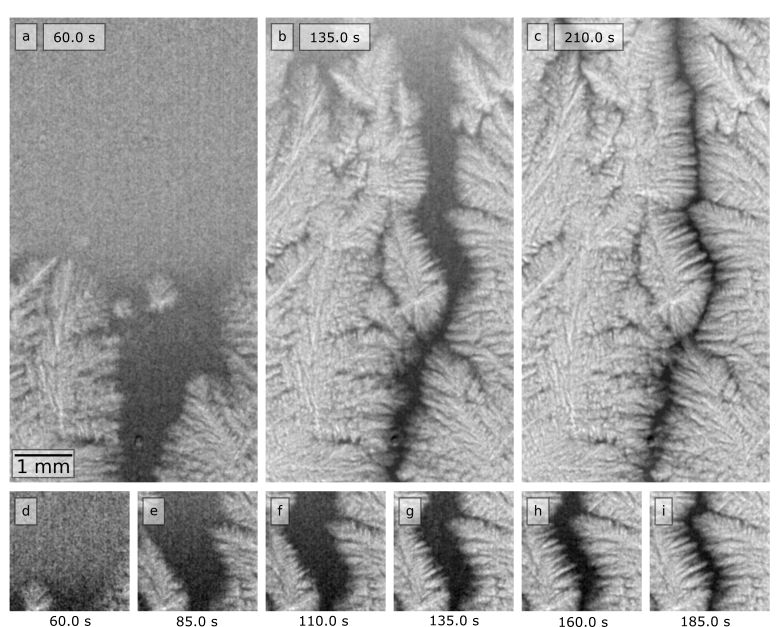
\includegraphics[width=0.6\textwidth]{figures/03/01-rad-seq.png}
    \caption{
        \small\setstretch{1}
        (a - c) In situ x-radiographs showing the mesoscale solidification of
        an Al-9.68 Ag at.\% sample, with time shown in seconds passed since the
        start of solidification within the viewing window.
        (d - i) Additional frames for a region of interest in the middle
        right of the full sample. Lighter regions are Al-rich, whereas darker
        regions are Ag-rich.
    }
    \label{fig/03/rad-seq}
\end{figure}

% -------------------------------------------------------------------------
\subsubsection{Backscattered Electron Image Comparison}
% -------------------------------------------------------------------------
Multiple post-solidification BSE images were used to create a single BSE
image montage for comparison with the x-radiography data at the end of
solidification (Fig. \ref{fig/03/sem-rad}).
Because BSE signal intensity increases with Z \cite{Reuter2003},
regions of high Ag concentrations are represented by lighter areas in the
image, while darker areas represent low Ag concentrations. This being the
case, it is reasonable to conclude that the small pits observed in very
light regions inherited high Ag contents (e.g., from enriched
interdendritic liquid) relative to their surroundings, leading to
corrosion during polishing. In the radiographs, the intensity relationship
is reversed because regions of high Ag decrease the transmission of
x-rays, resulting in darker pixels. Despite differences in spatial
resolution and signal depth between these two techniques, the BSE images
(\ref{fig/03/sem-rad}.a, b) are perceived as inverted relative to the
x-radiography (as expected). To allow for a clearer comparison,
an inverted BSE image is included (\ref{fig/03/sem-rad}.c)
to show the similarities in the solidified features
with the fully solidified x-radiograph (\ref{fig/03/sem-rad}.d).
This observation highlights the fact that Z values have a strong influence on
contrast in x-radiography.

\begin{figure}[ht]
    \centering
    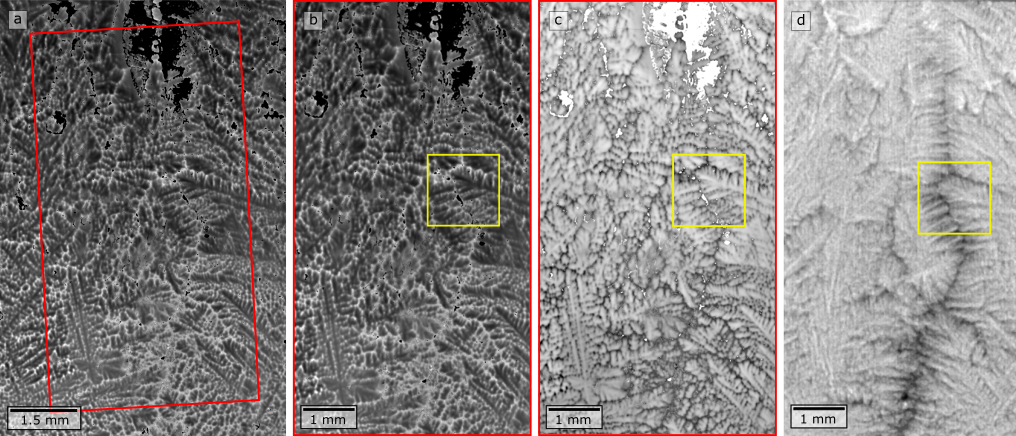
\includegraphics[width=0.6\textwidth]{figures/03/02-sem-rad.png}
    \caption{
        \small\setstretch{1}
        (a) Post-solidification BSE image montage with the area of the
        sample analyzed through in situ x-radiography indicated by the red
        overlay.
        (b) BSE image rotated and cropped to the x-radiography analysis
        area with the yellow overlay corresponding to the region of interest in
        \ref{fig/03/rad-seq}.d - i.
        (c) BSE image with grayscale values inverted to facilitate
        visual comparison to x-radiography with the region of interest once
        again indicated by the yellow overlay.
        (d) X-radiograph of the fully solidified
        sample (939 s after the start of solidification). Yellow overlay
        corresponds to the same region of interest as in (b) and (c).
    }
    \label{fig/03/sem-rad}
\end{figure}

% -------------------------------------------------------------------------
\subsubsection{Solidification Calculation Comparison}
% -------------------------------------------------------------------------
Following the frame progression during solidification in
\ref{fig/03/rad-seq}.d - i, the first solid to form is a light-colored
dendrite. According to the phase diagram (\ref{fig/03/sem-rad}.a),
this primary solid is expected to have a low Ag
content, which causes the interdendritic fluid to become enriched with Ag.
As solidification continues, Ag concentrations in both the recently frozen
solid and the remaining liquid increase as the Al-rich solid continues to
partition Ag into the liquid. The Scheil solidification model is shown and
compared with the evolution of the fraction of phases using an equilibrium
(lever rule) solidification path (\ref{fig/03/sem-rad}.b).

\begin{figure}[ht]
    \centering
    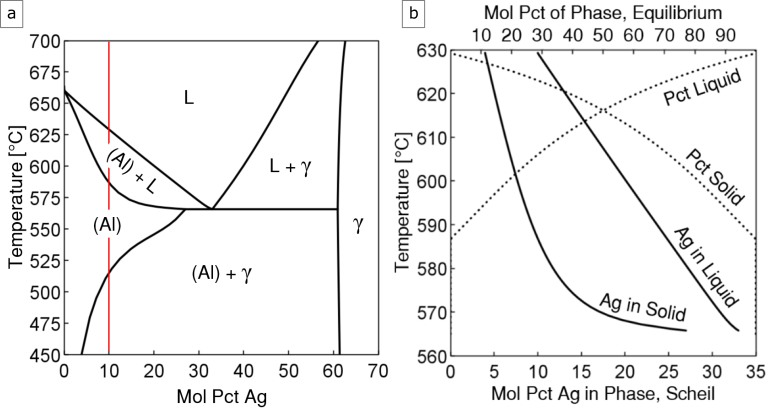
\includegraphics[width=0.6\textwidth]{figures/03/03-phase-scheil.png}
    \caption{
        \small\setstretch{1}
        (a) An equilibrium Al-Ag phase diagram with the sample composition
        (Al-9.68 Ag at.\%) indicated by a red line.
        (b) Thermo-Calc solidification calculations showing Ag concentrations
        in the liquid and solid phases (Scheil, solid lines) and phase
        percentages (Equilibrium, dotted lines).
    }
    \label{fig/03/phase-scheil}
\end{figure}

In the Scheil calculation results (\ref{fig/03/phase-scheil}.b),
as expected from the phase
diagram, Ag concentration is found to increase for both the liquid and
solid phases during solidification, and the solidus temperature is reduced
from the equilibrium value of 587°C to the eutectic temperature at around
566°C, as indicated by the ends of the Scheil curves (solid lines)
compared to the equilibrium fractions (dotted lines). At this temperature,
the Scheil model indicates that the remaining liquid reaches the eutectic
point (33 mole percent Ag) and solidifies as an (Al + $\gamma$) microconstituent.
The trend of progressive Ag enrichment in the liquid phase is consistent
with the BSE images and x-radiographs.

The results obtained from the Scheil calculations can also be compared
directly to the radiographs by measuring the fraction solidified at
different times during solidification. Using Python, solid regions were
identified and manually labeled by tracing the solid structures on label
layers in the napari image viewer. This created binary mask images which
were overlaid on each other to show the progression of the solidification.
These binary masks were then analyzed using the measure submodule of
scikit-image to compare the area solidified of each image to the total
area of the images. At this point, the as-measured fraction solid, with
each image representing different solidification temperatures, was
compared to the Scheil simulation results expressed as fraction solid and
temperature. By aligning the as-measured fraction solid with the Scheil
calculated fraction solid, a mapping was made from solidification
temperature (position in image sequence) to solid composition
(\ref{fig/03/solid-frac}.a).
The measurement of fraction solid does not continue for the full range of
solidification because the solidification occurred slowly at the end of
the experiment, so the best fitting portion of the Scheil simulation also
does not reach complete solidification. This image number to solid
composition mapping from the Scheil simulation at any given instant was
then used to estimate the concentration of the solid formed between two
successive radiographs, ultimately constructing a spatiotemporal solute
microsegregation map (\ref{fig/03/solid-frac}.b).

\begin{figure}[ht]
    \centering
    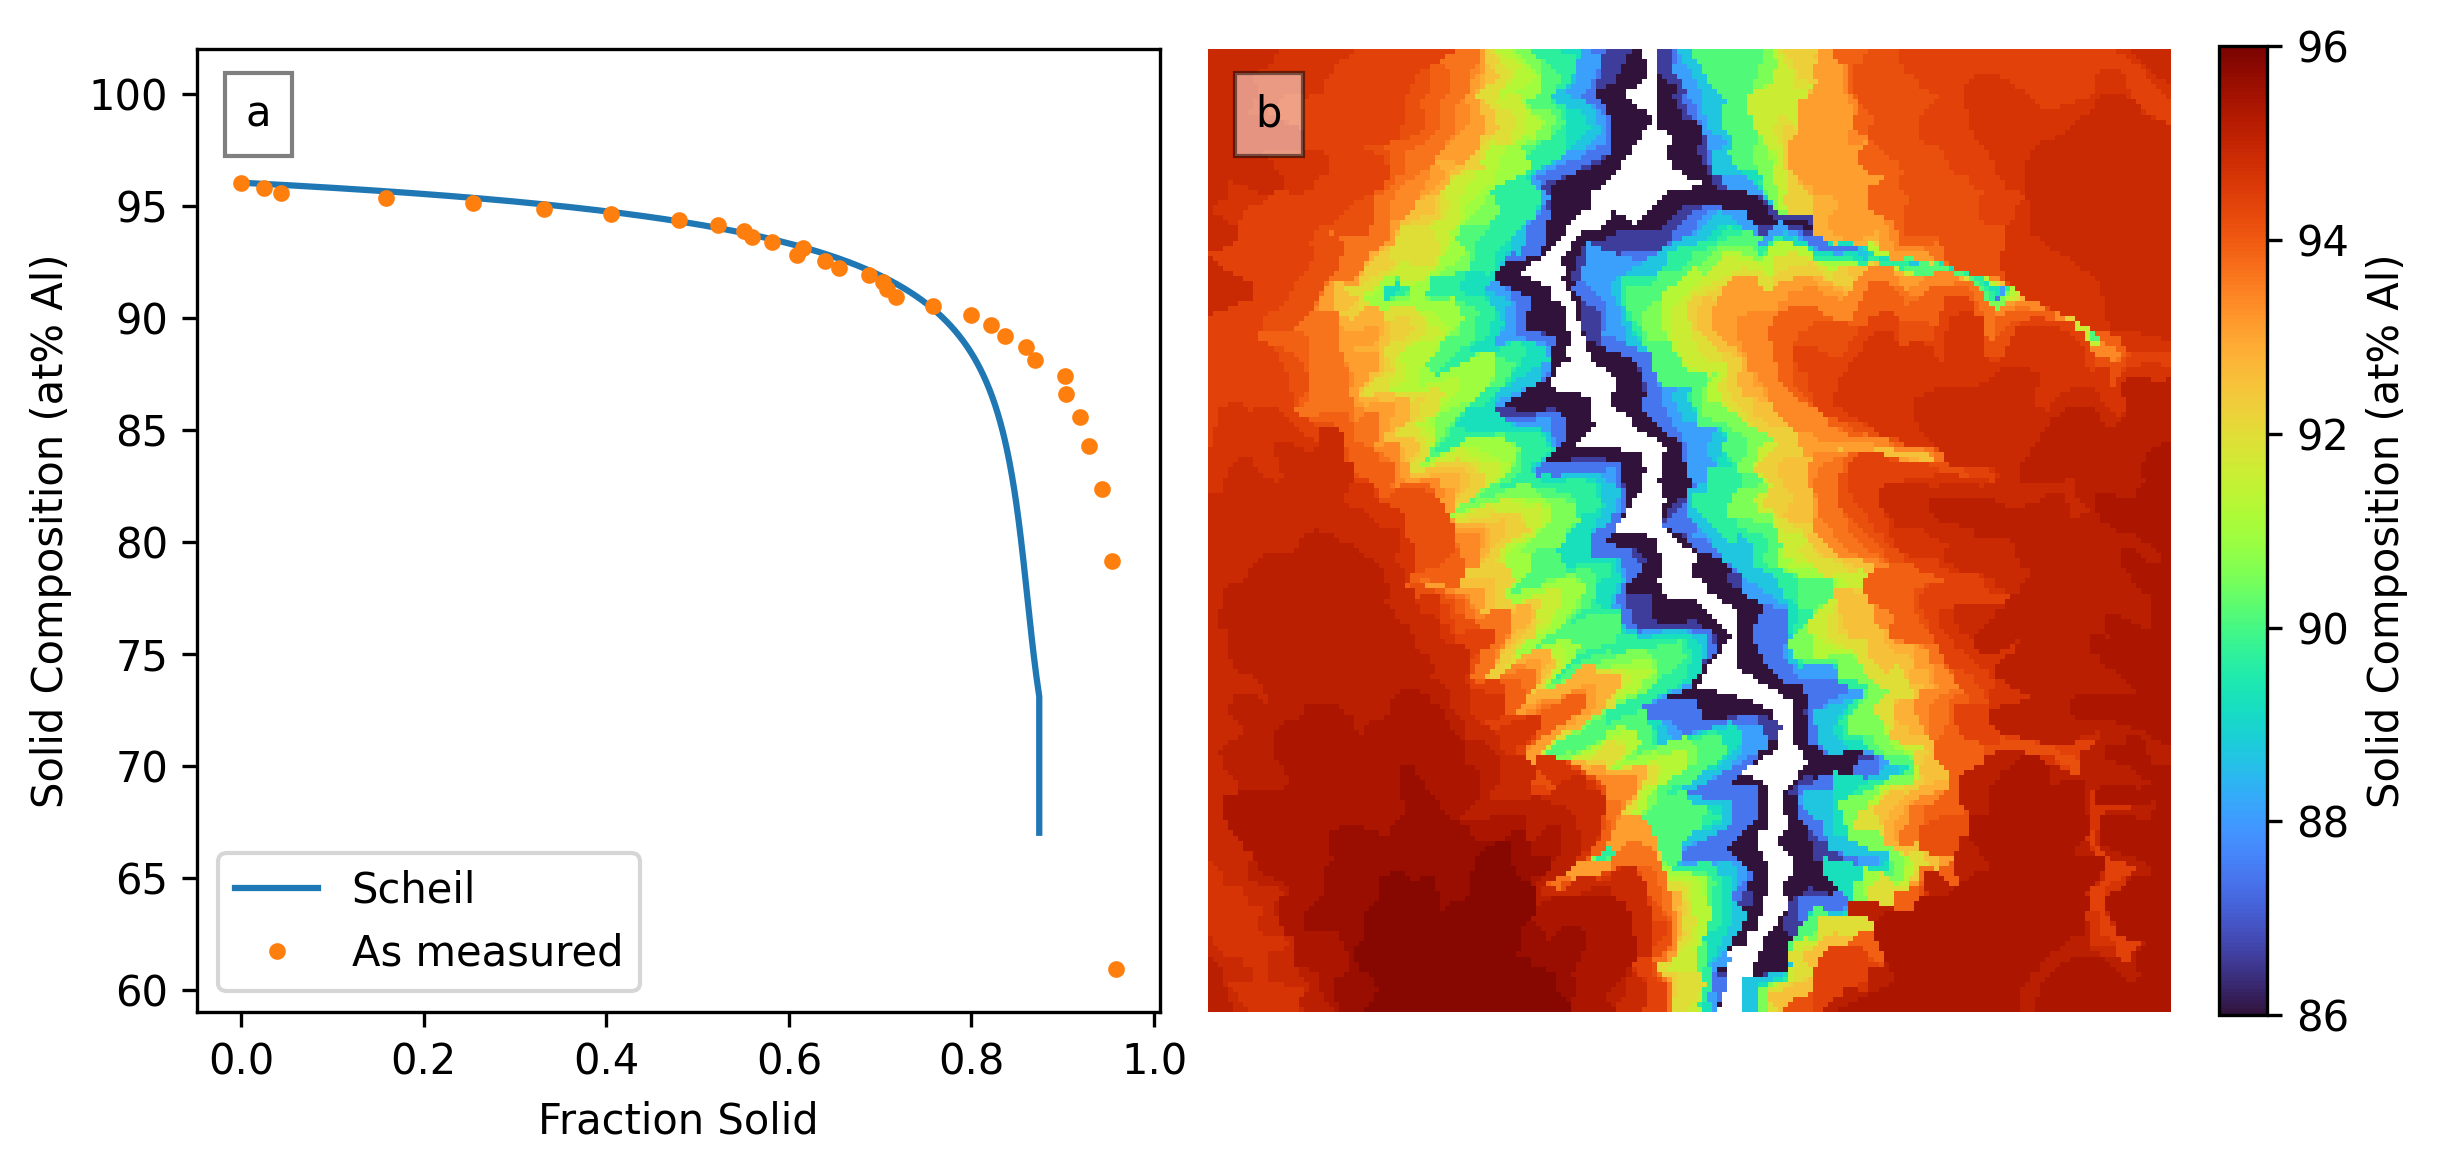
\includegraphics[width=0.6\textwidth]{figures/03/04-solid-frac.png}
    \caption{
        \small\setstretch{1}
        (a) Comparison between the Scheil solidification simulation results
        expressed as solid composition versus fraction solid (blue) and the
        Scheil solid composition data mapped to the fraction solid as measured
        in this region of the radiographs (orange).
        (b) Mapping fraction solid to composition of the solid at the point
        of solidification (at\% Al) during in situ x-radiography. Color
        represents decreasing Al content of the solid forming during
        solidification.
    }
    \label{fig/03/solid-frac}
\end{figure}

Using this matching procedure between Scheil simulation results and
radiographs, which is based on the observable solid fraction, the
agreement between simulation and experiments lead to a good match
(\ref{fig/03/solid-frac}.a) for most of the freezing range, with some
deviation at high solid fraction.
This is directly due to a discrepancy in solid fraction between
model and experiments: given the underlying assumption that the cooling
rate is homogeneous and constant, temperature (simulation) and time
(x-radiography) axes are thus kept linear with respect to each other,
which in turn results in the deviation in fraction versus composition
estimation at high solid fraction (\ref{fig/03/solid-frac}.a).
This discrepancy could, to
some extent, be addressed by relaxing the assumption of homogeneous and
constant cooling rate, allowing it to deviate from this ideal case locally
(in time and space), for instance, by directly using the concentration
versus solid fraction curve from the CalPhaD calculation to estimate the
concentration profile (instead of the solid fraction versus time and/or
temperature). Another possible source of error stems from how the fraction
solid was measured in the radiographs. Since the x-rays travel through the
entire volume of the sample, liquid trapped between dendrites or dendrites
that form but do not span the entire thickness of the sample could be
measured as a fully solid area, even though they represent a volume that
may not be completely solid. Additionally, only a single region of
interest of the sample is analyzed in this way, so it is also possible
that this region is not completely representative, as some solute may
enter and exit this region to other portions of the sample, and
temperature may also vary beyond this region. While the current 2D
analysis already provides a reasonable estimation of the solid fraction,
it might be further enhanced using contrast-based volumetric
reconstruction through the sample.35 An important feature of the
microsegregation analysis technique proposed here is that, while
approximate and relying on strong assumption (e.g., CalPhaD-based
solidification path), it is straightforward to extend to multicomponent
solute mapping. This would be impossible to obtain through radiography
analysis alone and could provide an important tool for further analysis of
time-dependent in situ imaging data.

% -------------------------------------------------------------------------
\subsubsection{Comparing EDS and x-Radiography}
% -------------------------------------------------------------------------
Comparisons between the EDS-determined compositions and the radiograph
intensities can be made, despite differences in the techniques for
collecting these datasets. These comparisons were made by using Python and
the napari image viewer to manually overlay the BSE montage image, the
individual BSE images containing the overlay of the line scan locations,
and the x-radiograph showing the fully solidified structure. With these
images aligned, a line could be placed on the x-radiography in the
location corresponding to the EDS line scan, such that the corresponding
pixel intensity of the x-radiograph could be determined. While pixel
intensities in x-radiography convey information about composition due to
varying Z of the material in the sample, the intensities also convey
information about the entire thickness of the sample. This is contrasted
with the volume sampled by EDS, which is only on the order of 3 µm from
the metallographically prepared surface (approximately 30 µm below the
surface of the as-solidified sample). Since this volume is about two orders
of magnitude smaller than the volume probed by x-radiography
(already the small approximately 250 µm thickness), the EDS is more akin to
an analysis of the surface. These differences need to be considered when
comparing the data. A comparison of an EDS line scan showing the Al content
over the length of the line shows similar trends to the x-ray intensity
profile of a line in the same location on the aligned radiograph
(\ref{fig/03/eds-vs-rad-1}).

\begin{figure}[ht]
    \centering
    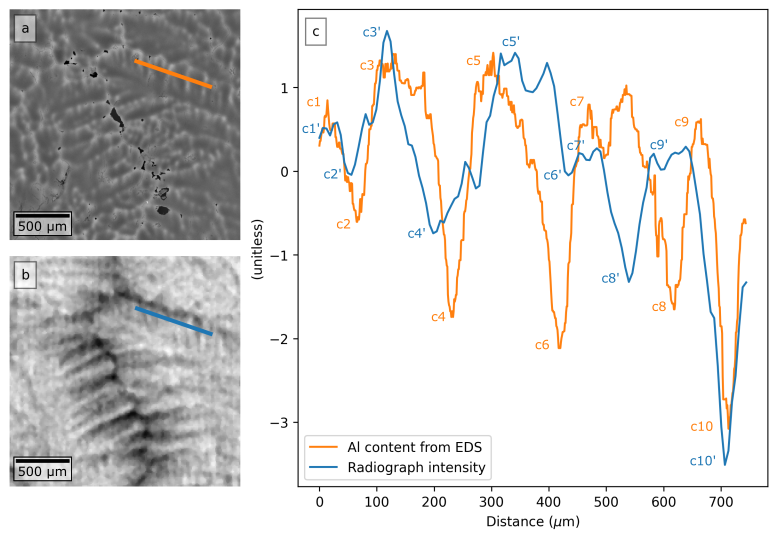
\includegraphics[width=0.6\textwidth]{figures/03/05-eds-vs-rad-01-09.png}
    \caption{
        \small\setstretch{1}
        (a) BSE image of an Al-Ag sample showing the position of an EDS
        line scan measuring the Al content.
        (b) X-radiograph of the same sample region, post-solidification.
        (c) Al content from the EDS line scan (orange) and the transmitted
        x-ray intensity (blue), collected across the length of the lines in
        (a) and (b) respectively. Each dataset is standardized to a unitless
        range for comparison. EDS features annotated as c1 - 10 correlate to
        x-radiography features annotated as c1' - 10', respectively.
    }
    \label{fig/03/eds-vs-rad-1}
\end{figure}

Annotations along the datasets in \ref{fig/03/eds-vs-rad-1}.c show
features consistent across
the length of the line across the sample for both EDS and radiography. The
line is oriented such that the beginning is near the tip of a primary
dendrite, traveling along the secondary dendrite arms towards the areas
that were first to solidify. Many correlated features exist between these
datasets, such as the maxima annotated in \ref{fig/03/eds-vs-rad-1}.c
as c1 and c1', c3 and
c3', and c5 and c5', and the minima annotated as c10 and c10'. Differences
between the datasets can be reasonably explained considering the nature of
the acquisition techniques. One way these discrepancies could manifest is
through local maxima or minima in the datasets not centered at the same
location along the lines. Volume measurements captured by x-radiography
are expected to deviate from the surface measurements captured by EDS in
the case when a given feature in the sample (e.g., a secondary dendrite
arm) may not be oriented in a way that places its center of volume
directly in line with the cross-section measured at the surface by EDS.

Another manifestation of the discrepancies that arise due to the
differences in volume versus surface effects of these two modes of
analysis is considered in the region of the sample analyzed across
well-defined secondary dendrite arms (\ref{fig/03/eds-vs-rad-2}).
The EDS and radiograph profile data is normalized in the same way as in
\ref{fig/03/eds-vs-rad-1}, and, although we
see correlations between the minima and maxima of the datasets, the
general trend across the entire length of the EDS data exhibits maxima and
minima (corresponding to Al-rich dendritic and Ag-rich interdendritic
regions, respectively) at similar intensities
(orange line, \ref{fig/03/eds-vs-rad-2}.c). In
contrast, the x-radiography intensity (blue line) progressively increases
across the length of the line.

\begin{figure}[ht]
    \centering
    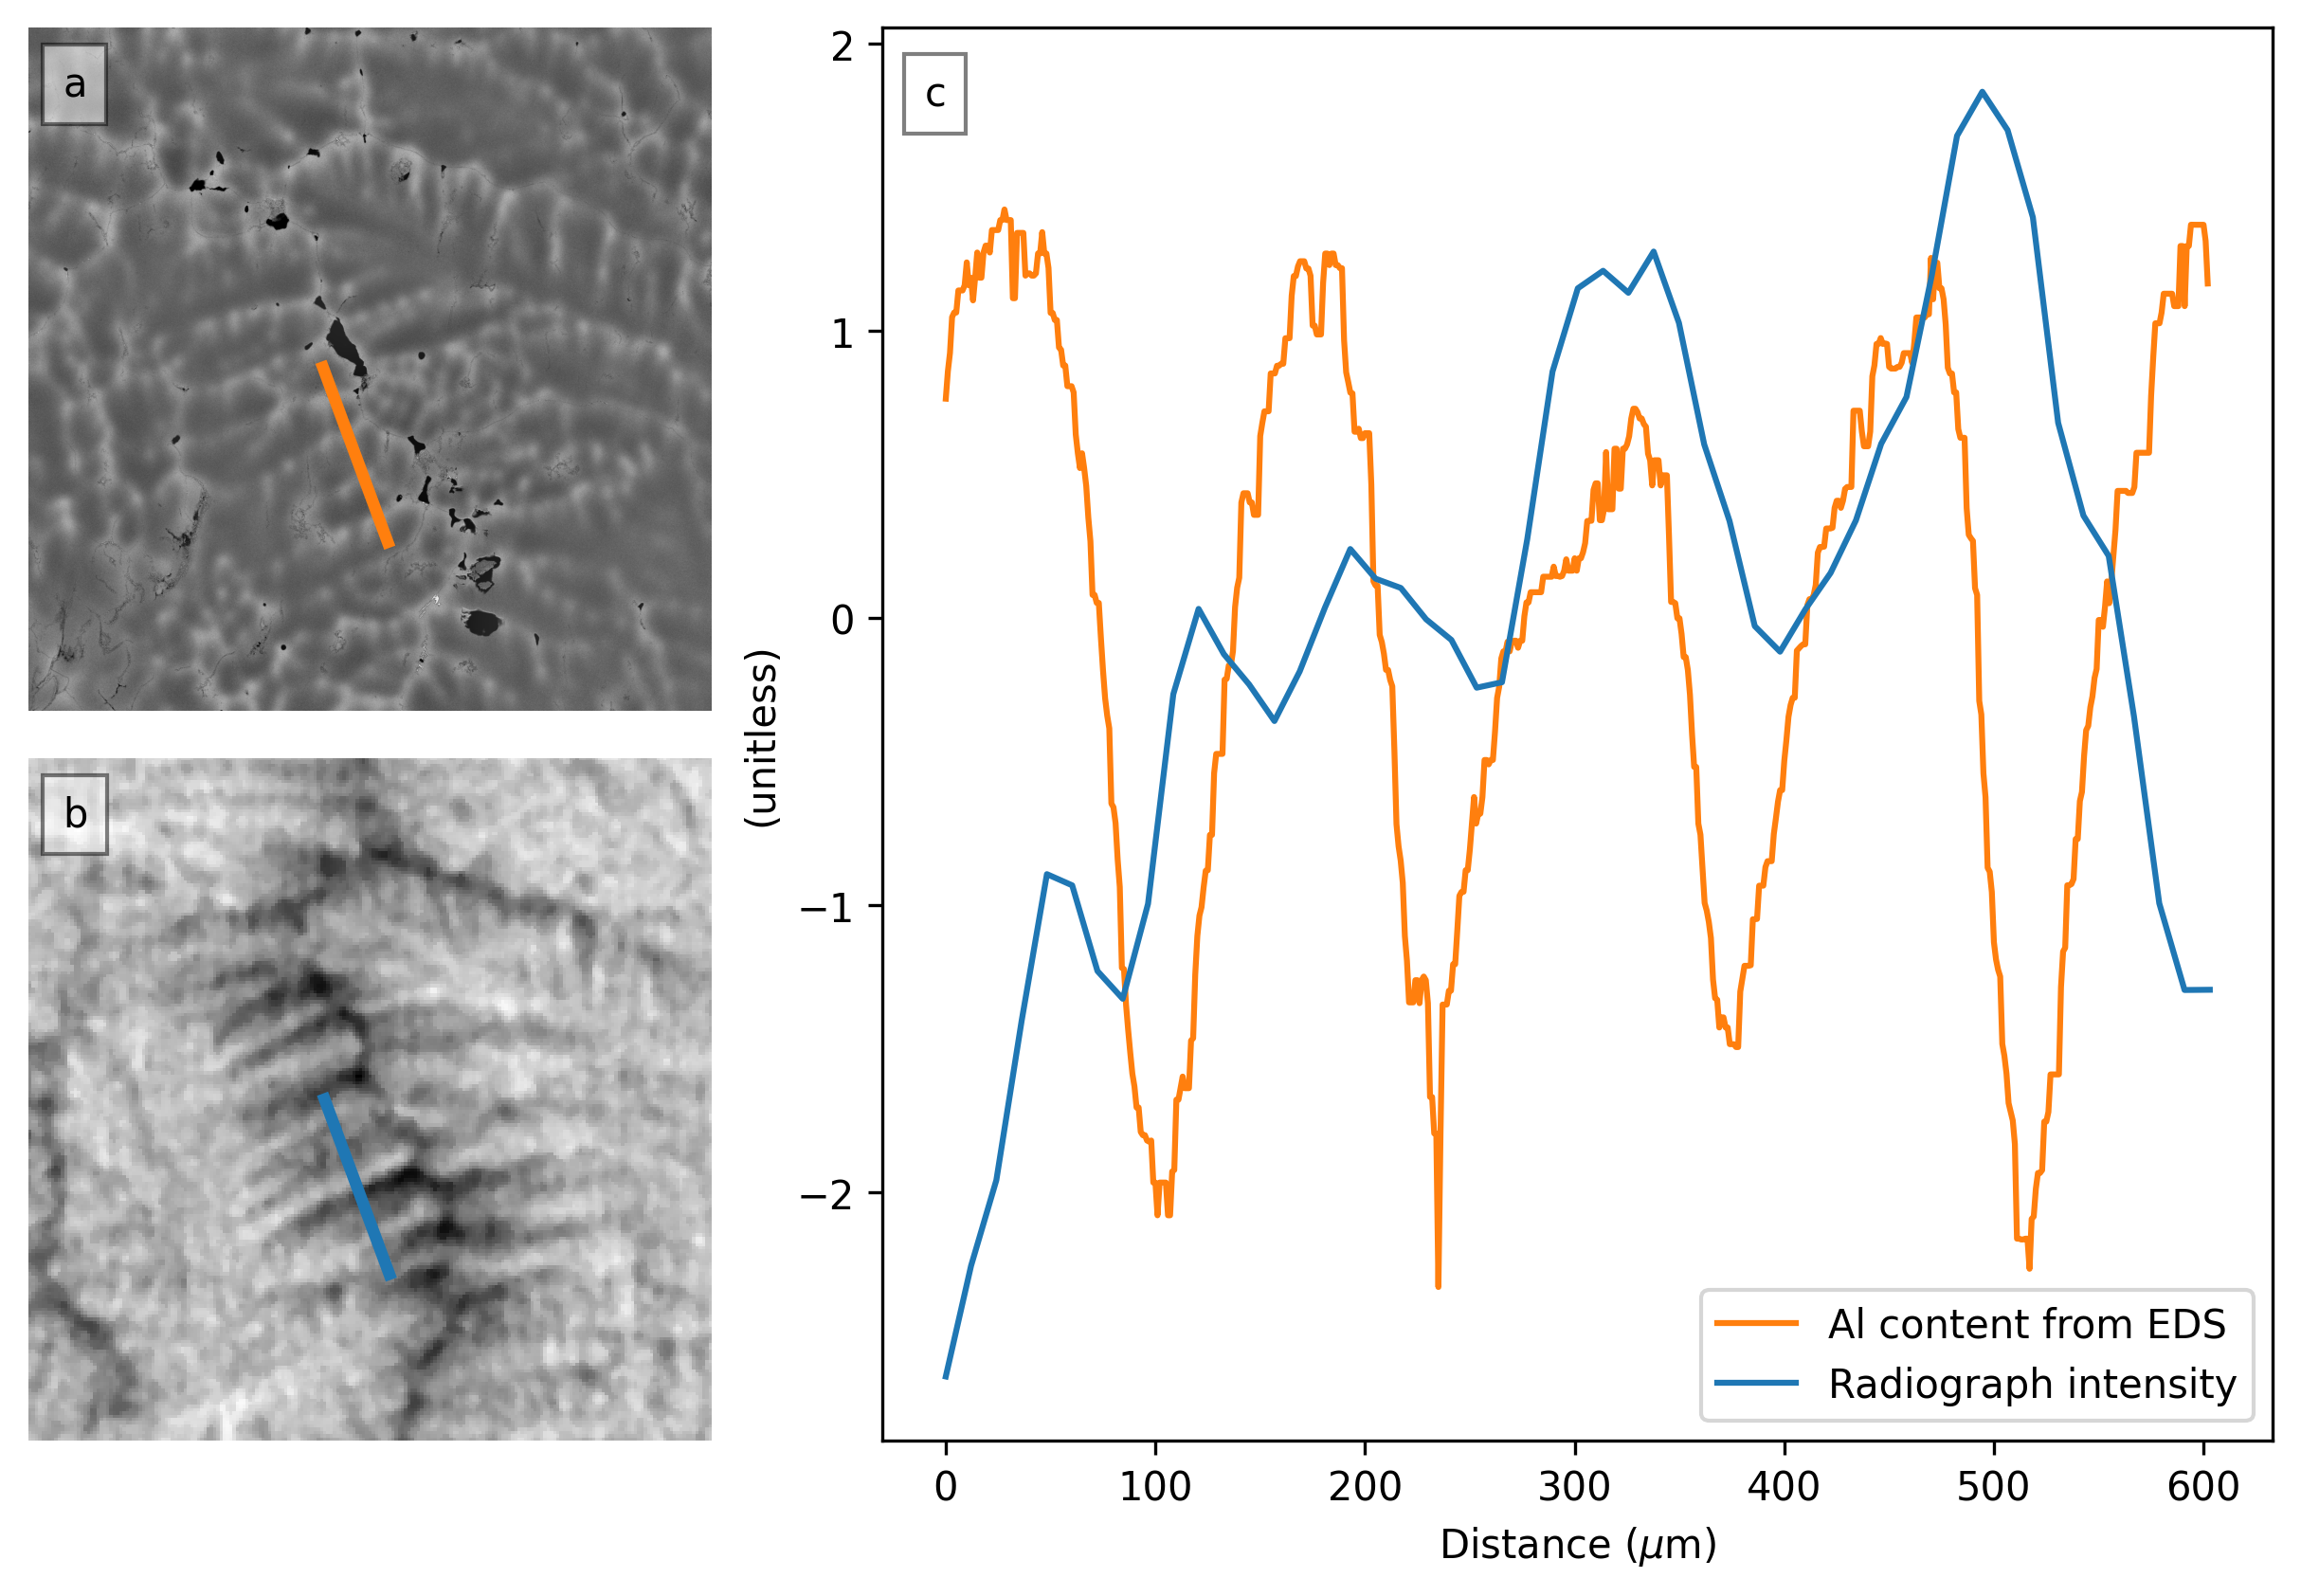
\includegraphics[width=0.6\textwidth]{figures/03/06-eds-vs-rad-05-17-1.png}
    \caption{
        \small\setstretch{1}
        (a) BSE image of an Al-Ag sample showing the position of an EDS
        line scan measuring the Al content.
        (b) X-radiograph of the same sample region, post-solidification.
        (c) Al content from the EDS line scan (orange) and the transmitted
        x-ray intensity from the x-radiograph (blue). Each dataset was
        standardized to a unitless range for comparison, with data collected
        across the length of the lines in (a) and (b), starting at the top
        left endpoint of the line and moving towards the bottom center of
        the images.
    }
    \label{fig/03/eds-vs-rad-2}
\end{figure}

One possibility for this discrepancy could be the decreasing thickness of
the dendrite arms along the length of the line, rather than composition
differences. Progressively increasing intensity in x-radiography data
corresponds to progressively higher transmission of x-rays. Hence, the
secondary dendrite arms further along the length of the line of analysis
could be progressively thinner, allowing for more x-rays to be
transmitted. This may not be visible at the surface after solidification
is complete (and therefore would not show in the EDS data). Even if the
dendrite arms were the same size and shape, differing orientations with
respect to each other could still cause the dendrite arms to have more
volume in the path of the x-rays.

Another possibility that may explain some mismatch between the datasets is
the existence of multiple layers of dendrites or of sidebranches within
the sample thickness. In the annotations of
Fig. \ref{fig/03/eds-vs-rad-2}.c, most of the features
of the EDS data are seen to correlate with the x-radiography, except for
the feature annotated as c3. In the radiography, c3' consists of two
separate peaks, whereas, in the EDS, what we see can be considered a
higher single peak (with some noise). Possibly, a secondary dendrite arm
between the two EDS maxima c1 and c3, but below the surface, such that it
would be behind these other two surface dendrites, could lead to this
additional local maximum in the radiography data, whereas it would remain
undetectable from surface analysis. When we compare the areas around the
length of the line on the SEM image (Fig. \ref{fig/03/eds-vs-rad-2}.a) and
the radiograph (\ref{fig/03/eds-vs-rad-2}.b),
we see the correlation between dendrite arms c1 and c1'; however, the
interdendritic region c2 and the following dendrite arm c3 are clear in
the EDS data, but neither c2' nor c3' is clear in the radiograph.
Solid-state diffusion is another possibility to alter the compositions of
the final, as-solidified microstructure measured by EDS, relative to those
that exist just after solidification and observed by radiography.

While direct comparisons between x-radiography and EDS remain challenging,
especially due to differences arising between the volume-probing nature of
x-radiography and the surface analysis nature of EDS, the combination of
these characterization methods enables relative changes during materials
processing to be analyzed in a laboratory setting. Three-dimensional
analysis, such as 3D computed tomography, could be considered as an
additional concurrent data source, which would support or discard such
interpretations of through-thickness features in the sample. Future work
and some of the potential exploration pathways deriving from this work are
briefly mentioned in the following section.

% -------------------------------------------------------------------------
\subsubsection{Perspectives}
% -------------------------------------------------------------------------
Combining both in situ and post-solidification diagnostics, as well as
modeling and simulation tools, offers many exploration pathways for
ongoing and future work. Using CalPhaD alone, several ways of
reconstructing the microsegregation profile may be envisioned, only one of
which has been illustrated here. Frameworks may be considered that would
for instance combine (1) compositional analysis directly from the
gray-level radiographs
\cite{Ruvalcaba2007,Bogno2011,Bogno2013,Becker2016a,Becker2020,Mirihanage2014}
(however, limited to binary alloys
for a semi-quantitative analysis), (2) microsegregation simulations using
different approaches, such as lever rule, Gulliver-Scheil, or models
accounting for finite diffusivities (e.g., using CalPhaD-based or other
volume-averaged methods \cite{Tourret2009}), and
(3) further post-solidification
compositional analyses, such as wavelength dispersive spectroscopy, the
amount of redundancy with EDS possibly being used as a cross-validation
tool or for more comprehensive analysis.

Combining in situ imaging data and simulations also provides numerous
promising avenues for data analysis of transient conditions during
solidification, and determination of physical parameters otherwise
extremely challenging to estimate, if measurable at all. One recent
example of such analysis is combined time-resolved 3D x-ray tomography
data with phase-field modeling of grain growth to extract grain boundary
mobilities and their orientation dependence over a statistically relevant
sample size \cite{Zhang2020}.
In the context of solidification, several crucial
parameters are particularly challenging to obtain, one example of which is
the anisotropy of solid-liquid interfacial properties like the excess free
energy and its anisotropy. In situ imaging could be combined with
corresponding simulations of microstructural evolution using phase-field
modeling at the scale of a representative volume element \cite{Mitsuyama2020}
or other ``mesoscale'' solidification simulations using, for instance,
envelope-based or needle-based approaches, providing further insight into
in situ data at the scale of entire experiments
\cite{Becker2020,Olmedilla2019}. A rigorous
integration of simulation and experiments will most likely involve the use
of advanced statistical analysis techniques for large and highly
multidimensional datasets, such as machine learning.


\subsection{Conclusion}
This work demonstrates a monitoring technique combining the mesoscopic,
volume-probing investigation of high-energy, microfocus x-radiography and
the microscopic, compositional analysis of SEM EDS, supported by Scheil
solidification calculations. In situ x-radiography can provide relative
composition and solid fraction evolutions by pixel intensity changes
during solidification, while post-solidification EDS can provide more
quantitative compositional information, but only after processing of the
material and with localized surface analysis. The pairing of the data
received through volume-probing x-radiography with compositional surface
analysis captured by EDS creates a multimodal montage of data that is
greater than the sum of its parts. The combination of these concurrent
datasets with modeling data, here illustrated using simple CalPhaD-based
Scheil calculations, could reveal nuances beyond those directly accessible
through either the imaging, compositional mapping, or simulations taken
separately. Further development and calibration of the techniques
illustrated here will allow for in situ compositional monitoring
capabilities of dynamic processing of metals within a laboratory setting.
Potential exists for a completely non-destructive, in situ monitoring
technique available in the laboratory, with which a sufficient number of
samples could be analyzed by x-radiography and EDS, supported by modeling
data and perhaps calibration experiments, to provide a comprehensive way
to capture important information about solidification dynamics.
Furthermore, a database could be created to link radiograph intensities
with EDS-derived compositions for enough relevant conditions (i.e., sample
chemistries and geometries, processing conditions, etc.), combined with
modern, fast-acting real-time post-processing (e.g., based on
machine-learning algorithms), such that compositions could be inferred in
situ with reasonable accuracy.

\subsection*{Acknowledgements}
The microfocus x-radiography was supported by
the US Department of Energy, Office of Science,
Basic Energy Sciences under award no. DESC001606.
The SEM EDS and preparation of this
manuscript were supported by the US Department
of Energy, Office of Science, Basic Energy Sciences
under award no. DE-SC0020870.
Los Alamos National Laboratory is operated by Triad National
Security, LLC, for the National Nuclear Security
Administration of US DOE (Contract No. 89233218CNA000001).
The Tescan dual-beam FIB was funded through the support of the National
Science Foundation (DMR-1828454). Many of the
figures in this text were generated using Python \cite{python},
Matplotlib \cite{matplotlib}, and the open-source vector editing
software InkScape \cite{inkscape}.



% -------------------------------------------------------------------------
%   Chapter 4
% -------------------------------------------------------------------------
\newpage
\chapter{
    PROCEDURALLY DETECTING SOLID-LIQUID INTERFACES DURING SIMULATED ADDITIVE
    MANUFACTURING AND RAPID SOLIDIFICATION} \label{ch/melt}
% \section{Abstract}
In this chapter, procedures for detecting metallic melt pools are
presented to automate the
process of obtaining real-time solidification velocities to enable
comparisons to process modeling and microstructural outcomes predicted by
solidification theory and modeling. Procedures are developed to analyze
two types of solidification experiments: simulated metal
additive manufacturing (AM) of Ni-1.9 Mo-6.6 Al (wt.\%)
single crystals captured with x-radiography at the Advanced Photon Source
(APS) synchrotron facility at Argonne National Laboratory (ANL) and rapid
solidification of Al-3 wt.\% Si thin films captured with dynamic transmission
electron microscopy (DTEM) at Lawrence Livermore National Laboratory
(LLNL). Each procedure differs due to the nature of the experiment, but
each utilizes common Python libraries including \textit{NumPy},
\textit{imageio}, \textit{scikit-image}, and \textit{napari},
to perform steps including denoising, pseudo-flat-field intensity
correction, segmentation, and optimization of ellipse fitting.
The procedures are applied to three experiments of each type and the
detected melt pool evolution is compared with
manual measurements to show that the procedures are reasonably accurate.
The AM simulator procedure is more prone to inaccuracies due to noise,
and therefore less reliable than the rapid solidification procedure, which
is more robust, partly due to a fit optimization step.


% -------------------------------------------------------------------------
\subsection{introduction}
% -------------------------------------------------------------------------
Metal additive manufacturing (AM) encompasses a promising collection of
manufacturing techniques in which metallic parts are created layer by
layer. These techniques can create parts with complex geometries that are
not achievable with more traditional, subtractive techniques
\cite{Chu2008}. However, these techniques are not without their own
challenges. AM-built parts often produce columnar dendrites during
solidification. These anisotropic microstructures can lead to hot tearing
\cite{Kaufmann2016,Martin2017,Gu2019}.
% and anisotropic material properties?
While there has been some success
leveraging anisotropy to intentionally localize properties in AM-built
parts \cite{Dehoff2015,Plotkowski2021}, isotropic microstructures are
usually preferred to reduce the tendency for cracks to form. This requires
the growth of equiaxed grains as opposed to columnar grains. Many methods
have been successful in encouraging equiaxed grain growth, including
alteration of alloy composition \cite{Spittle2013,Bermingham2019,Zhu2019},
addition of grain nucleating nanoparticles \cite{Martin2017,Gu2019}, changing
build height \cite{Qiu2015}, changing feedstock rate
\cite{Wu2004,Qiu2015}, and changing laser/electron beam processing
parameters like power \cite{Qiu2015,Balla2016,Kurzynowski2018}, scan speed
\cite{Wu2004,Qiu2015,Balla2016}, scan strategy
\cite{Dehoff2015,Kurzynowski2018}, and beam shape \cite{Roehling2020}.
A series of models have enabled studies of the effects of beam
processing parameters on melt pool dynamics and resulting microstructures.
The first of such models was developed by Hunt to analytically describe
the growth of equiaxed grains ahead of the columnar solid-liquid (S-L)
interface, shedding light on the columnar-to-equiaxed transition (CET)
\cite{Hunt1984}. This original CET model was developed for casting
applications, but the Kurz-Giovanola-Trivedi model describing rapid
solidification in the growth of columnar dendrites \cite{kgt1986} enabled
Gäumann et al. to extend Hunt's model to rapid solidification
\cite{Gaumann1997,Gaumann2001}. The latter work of Gäumann et al.
provided a simplified relationship between temperature gradient (G),
solidification velocity (V), and a material constant (K), which enables
predictions for when an alloy system undergoes equiaxed versus columnar growth.
Using this relationship, studies have predicted and verified
microstructures for varying processing parameters by comparing V, as
calculated from experiments, and G, as estimated with heat transfer
simulations in G-V maps
\cite{kgt1986,Kurz2001,Kurz2001b,Gaumann2001,Kobryn2003,Dehoff2015,Saville2021,Roehling2020,}.
These microstructure maps overlay experimental data with regions corresponding
to columnar, equiaxed, and mixed microstructures. Microstructure
maps can also be express process parameters directly, rather than G
and V, to determine combinations of processing parameters likely to
produce optimal microstructures \cite{Liang2016,Liang2017}.

With the opportunity to view melt pool evolution and development of
microstructures under AM-like conditions in situ comes the task of
tracking image features across the duration of solidification.
This feature tracking is often performed manually with some kind of
image viewing and annotation software like \textit{ImageJ} \cite{imagej}.
Manual tracking has been used to track droplet spatter
\cite{Leung2018nat,Leung2018am}, melt pool length/depth and overall area
shrinkage \cite{Leung2018am}, pores \cite{Leung2018nat,Martin2019}, vapor
depression/keyhole depth \cite{Martin2019,Cunningham2019}, powder motion
and spattering \cite{Guo2018}, melt flow within the melt pool via tracing
particles \cite{Hojjatzadeh2019}, and melt pool volume \cite{Guo2019}.

Most studies in literature do not explore automated methods of analyzing
melt pool features, although a procedural method for identifying interfaces
of melt pools has received a brief explanation in some studies
\cite{Zhao2017,Wolff2019}. In these studies, the interfaces
are identified on a row-by-row basis, based on local peaks in the second
derivative of the radiographs. This methodology is provided in the
supplementary materials, however, and no further explanation is given into
how the peaks of the derivatives corresponding to the interfaces are
selected from the other peaks present.

The goal of this work was to investigate the possibility of automating
analyses necessary to calculate solidification velocities for the
prediction of microstructure based on processing parameters. The
successful execution of this type of automation would remove some inaccuracies
related to human error and inconsistent subjective judgements across
different researchers, while also improving analysis efficiency. Automatic
analysis procedures are developed for two solidification experiments: an
AM simulator experiment and a rapid solidification experiment. The AM
simulator was developed at section 32-ID-B of the Advanced Photon Source
(APS) synchrotron facility at Argonne National Laboratory \cite{Zhao2017}
to simulate laser powder bed fusion (LPBF): an AM
technique in which material is fused together, one layer at a time, using
a high-energy laser \cite{King2015}. That said, the AM simulator may also be
used more generally to observe laser-substrate interactions (i.e., a
substrate without a powder layer).
Hard x-rays and high-speed x-ray detectors are used
to image the melting and solidification of Ni-1.9 Mo-6.6 Al (wt.\%)
single crystals in situ, revealing the melt pool such
that the S-L interfaces can be identified and tracked. The resulting location
information of the S-L interfaces are used to calculate solidification
velocities under LPBF-like conditions. The rapid solidification
experiments were performed by melting thin films
(approximately 100 nm in thickness)
of Al-3 wt.\% Si on an amorphous silicon nitride substrate and
monitoring the solidification using a dynamic transmission electron
microscope (DTEM) at Lawrence Livermore National Laboratory. DTEM has
proven to be useful in many rapid solidification studies
\cite{LaGrange2006,LaGrange2008,Kim2008,Campbell2010,Kulovits2011,LaGrange2012,Santala2013,McKeown2014,Zweiacker2015,LaGrange2015,Roehling2017,Ji2023}.
% Split this into many solidification experiments including x, y, z?
For each analysis procedure performed here, the automated measurements
are compared to manual measurements to assess the performance of the procedures.


\subsection{Methods}
% -------------------------------------------------------------------------
This section outlines the methods for performing the two types of
experiments presented in this work, developing
the procedures to automatically detect the solidifying melt pools as they
are observed, and the process for manually identifying the melt pools.
The presented procedures are written in the Python programming language
and formatted into \textit{Jupyter} notebooks \cite{jupyter}. Using Python
with \textit{Jupyter}
notebooks is beneficial for both development and presentation. The
cell-based nature of \textit{Jupyter} notebook files allow for an iterative
workflow for processing and analyzing data while also creating a
reproducible procedure in the process.
Variables declared in each cell are available to successive cells, allowing
for use of the same variables across a notebook, while showing the output of
a cell at any point of the procedure rather than at the end only.
Since cells can contain formatted text in
addition to code, scientific context can be provided about in addition to
technical information about the procedure itself in
between code cells, improving readability and reproducibility.
Other Python packages used in these procedures are
\textit{imageio} for reading and writing of image files \cite{imageio},
\textit{NumPy} for representing the images as numerical arrays and
performing fast calculations \cite{numpy}, \textit{scikit-image} for
performing image processing algorithms \cite{skimage}, and \textit{napari}
for visualizing and annotating the data with an interactive,
multi-dimensional image viewer \cite{napari}.

% -------------------------------------------------------------------------
\subsubsection{Ni-Mo-Al Simulated AM}
% -------------------------------------------------------------------------
Experiments simulating the processing conditions of LPBF were
performed using the AM simulator at sector 32-ID-B at the APS.
The simulator consists of an argon-backfilled chamber containing
a sample fixture holding a thin metallic plate sample
(approximately 100 µm thick) sandwiched between
two glassy carbon plates in the path of a polychromatic x-ray beam.
A 520 W laser is located above the sample. The
experiments are performed by striking the top surface of the metallic
sample with the laser, creating a pool of molten metal at the surface.
High-speed x-radiography captures the melting and solidification of the
sample with a downstream, high-speed detector. An image sequence through
time is captured with a spatial resolution of 1.93 µm
per pixel, a framerate of 80,000 frames per second, and a field-of-view of
988 by 741 µm. After the laser shuts off, the melted portion of the sample
(hereafter referred to as the melt pool) can be seen solidifying based on
the density and x-ray absorption differences between the liquid and the
solid phases (\ref{fig/rad-seq}).

\begin{figure}[ht!]
    \centering
    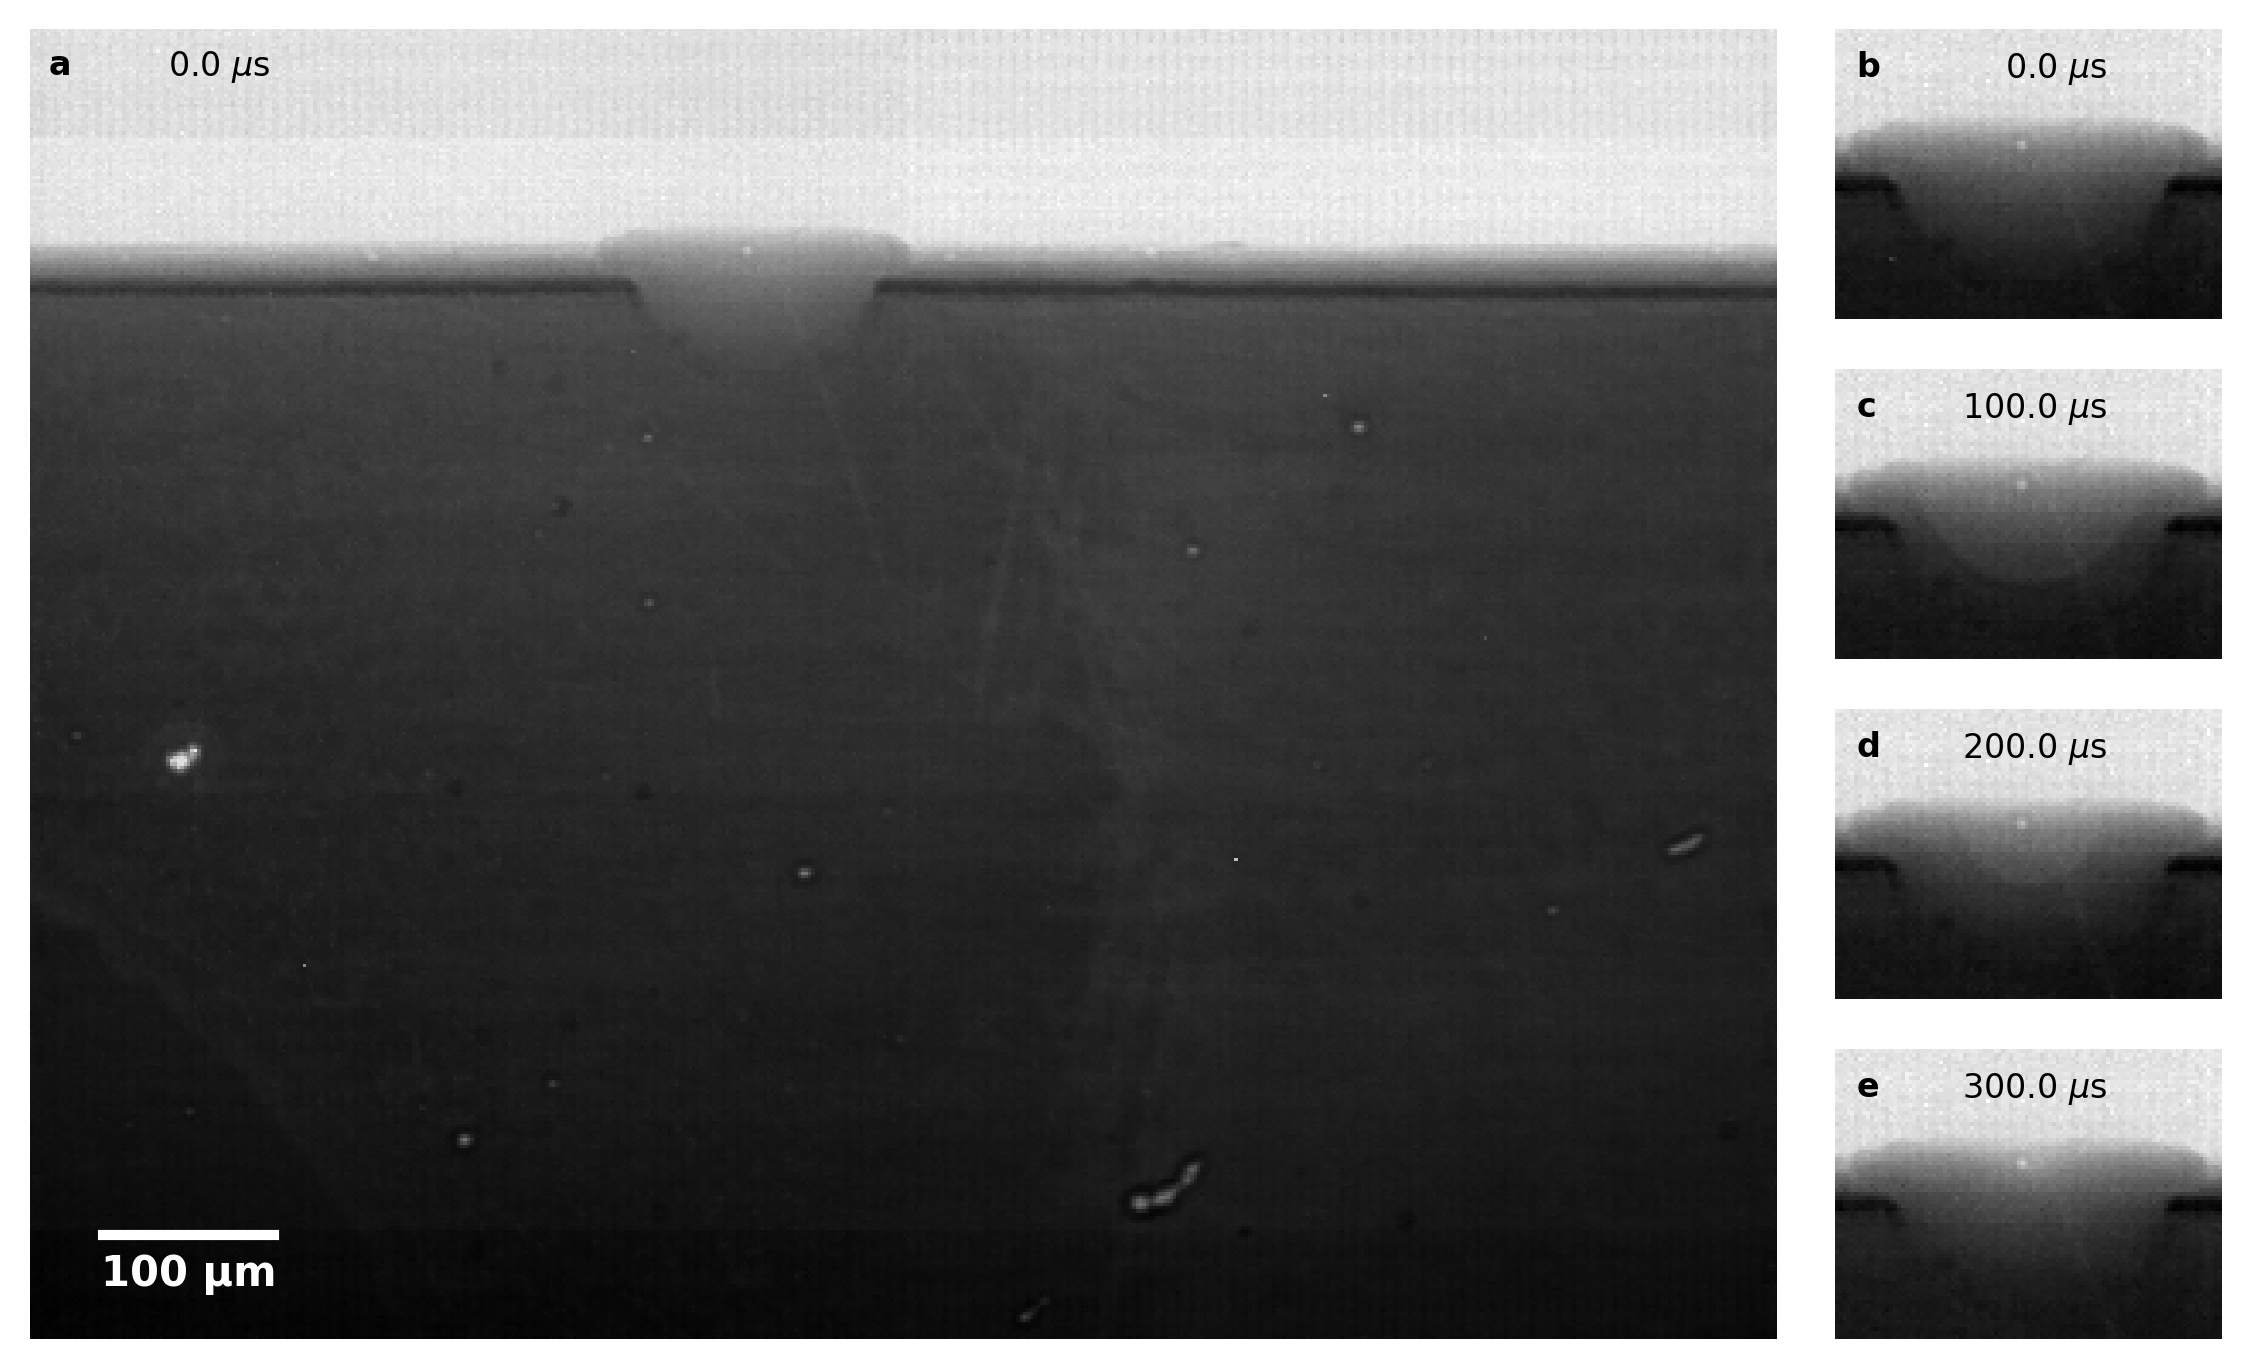
\includegraphics[width=0.75\textwidth]{figures/04/01-rad-seq.png}
    \caption{
        \small\setstretch{1}
        Subset of a time sequence of x-radiography depicting the solidification
        of a Ni-1.9 Mo-6.6 Al (wt.\%) single crystal after melting with a
        laser at 104 W (20\% maximum power).
        (a) Full image of radiograph right after the laser shuts off
        (t = 0 µs).
        (b) Radiograph from (a) cropped to the melt pool and immediate
        surroundings (t = 0 µs).
        (c) Cropped radiograph showing partial solidification and visible
        solid-liquid (S-L) interface (t = 100 µs).
        (d) Cropped radiograph showing further solidification and a smaller
        S-L interface (t = 200 µs).
        (e) Cropped radiograph showing near total solidification with S-L
        interface no longer easily visible (t = 300 µs).
    }
    \label{fig/rad-seq}
\end{figure}

\subsubsection{Simulated AM Detection Procedure}
% -------------------------------------------------------------------------
To measure solidification velocities during the AM-like process, the S-L
interface must be tracked through the radiograph sequence from the
experiment. Once the location is known, the change in location over time
yields the solidification velocity. To procedurally identify the S-L
interface, the images are processed in a way that highlights the
differences between each image and the preceding image in the time
sequence. The first step performed is the conversion of all images from
16-bit unsigned integer format to a floating-point image format
(\ref{fig/routine}.a). This changes the intensity range from
[0, 65536] to [0, 1] to enable floating point calculation and prevent a loss
of information from rounding to the nearest integer. Next, a
Gaussian filter is applied to each image. This smooths out noise in
the images. Each smoothed image is then subtracted from the succeeding
image (\ref{fig/routine}.b). The resulting subtracted image visually
highlights the moving
interface and some varying noise in the images, since it is these features
that are the areas of greatest difference in the sequence. The intensity
of the subtracted image is rescaled by clipping the intensity of the
image. This replaces the pixels with intensities in the upper and lower
fifth percentile with the intensity value at those cutoffs
respectively (\ref{fig/routine}.c).
The rescaled images are denoised using a total
variation minimization algorithm \cite{Kokaram2004} implemented in
\textit{scikit-image} as the function
\textit{restoration.denoise\textunderscore tv\textunderscore chambolle}.
This further reduces the intensity of the remaining noisy regions in
the image. The image is inverted so the regions
corresponding to the S-L interface region are represented by high
intensities in the image (\ref{fig/routine}.d). An upper minimum
threshold is applied to the inverted image to create a binary image
(\ref{fig/routine}.e). A skeletonization algorithm \cite{Zhang1984}
implemented in scikit-image as the function \textit{morphology.skeletonize}
is used to erode each connected region in the image to one-pixel wide
``skeleton'' regions in the binary image (\ref{fig/routine}.f).

\begin{figure}[ht!]
    \centering
    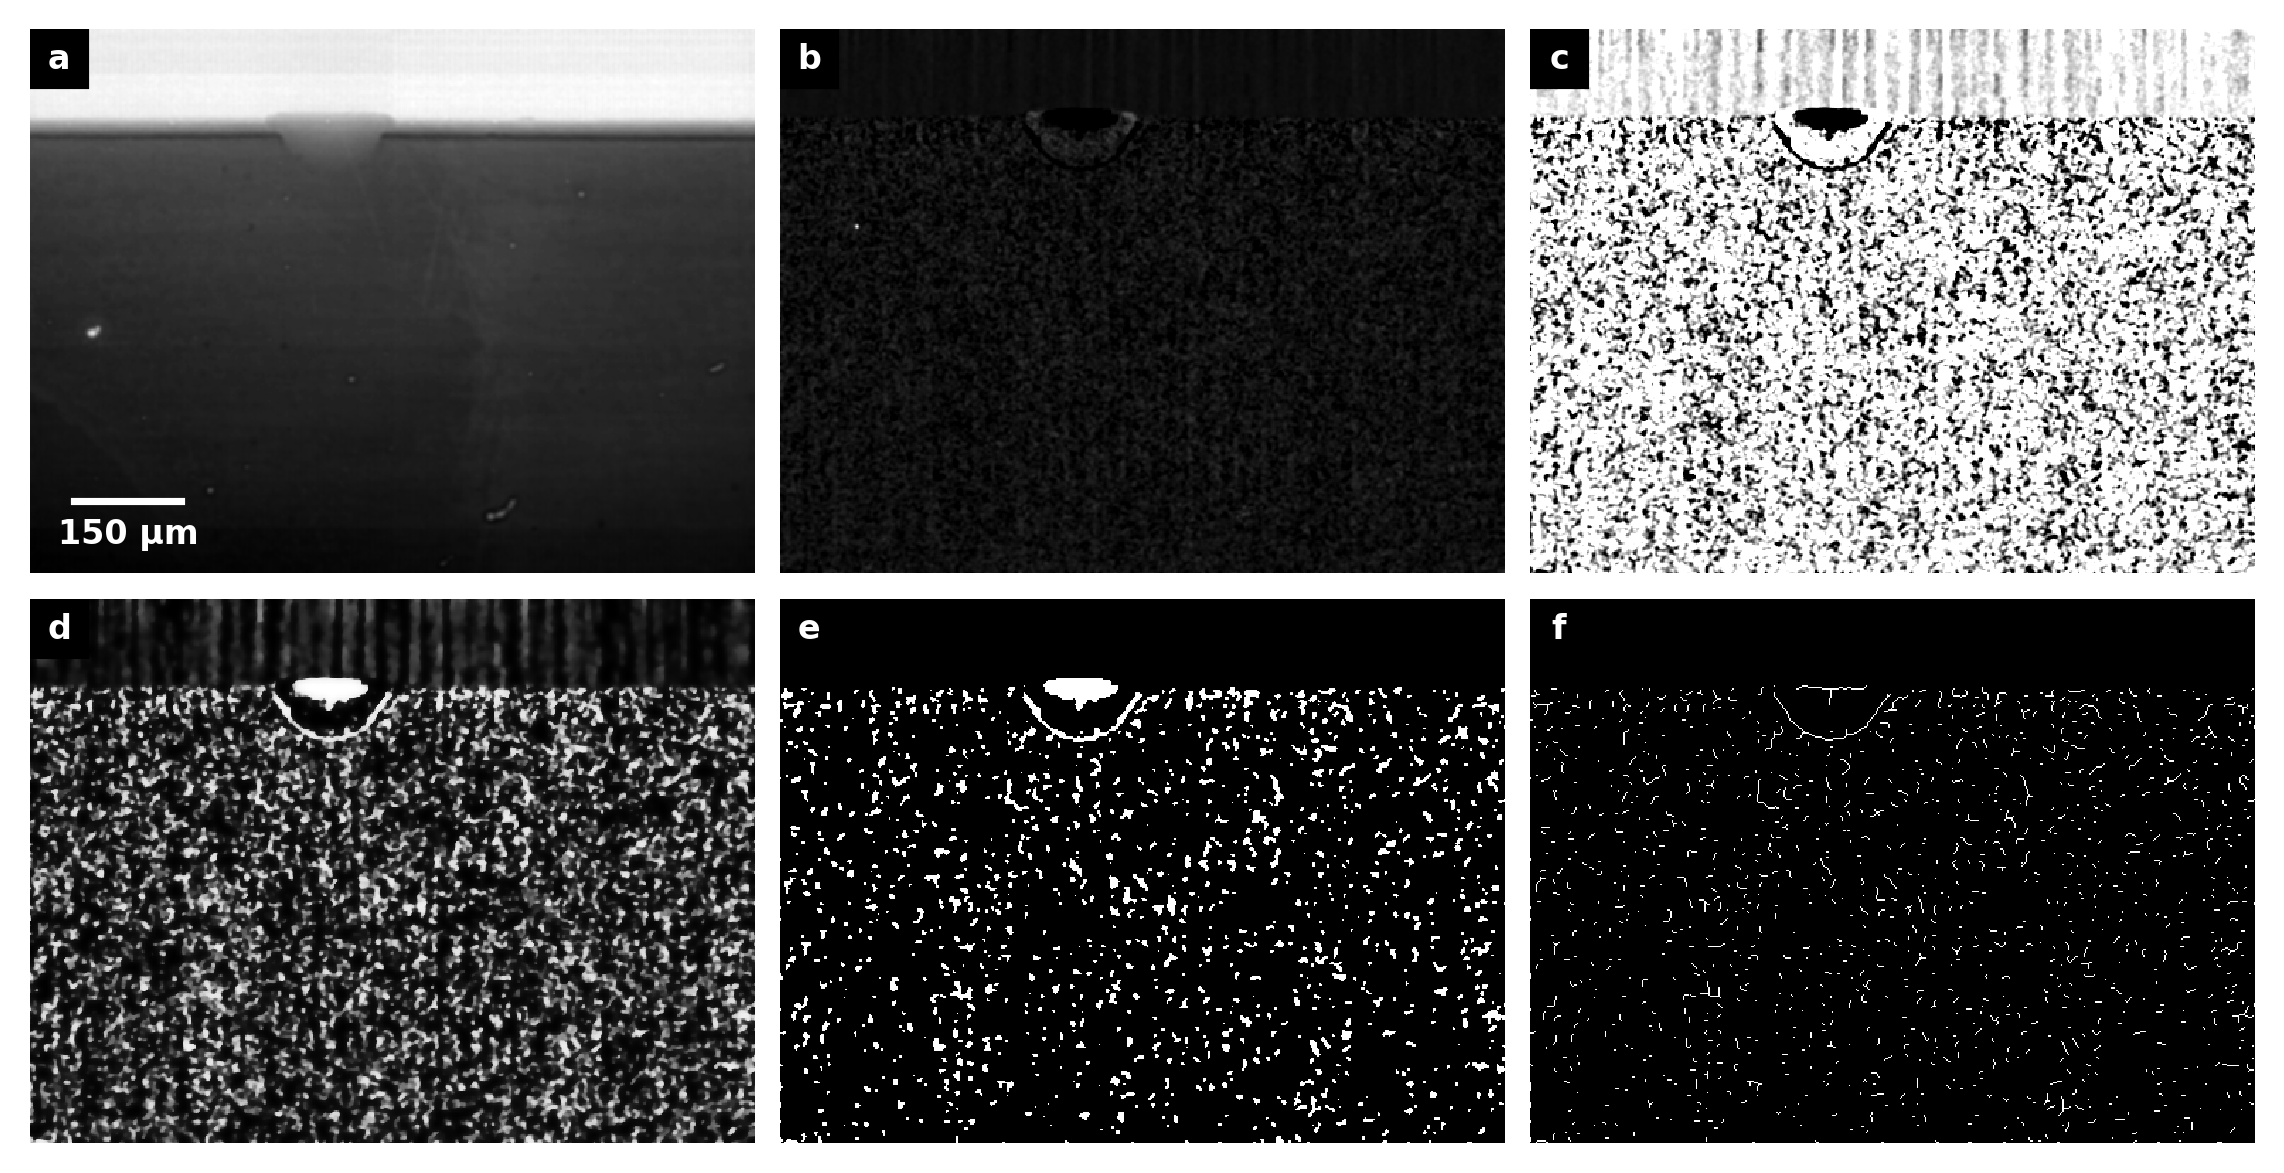
\includegraphics[width=0.75\textwidth]
    {figures/04/02-routine.png}
    \caption{
        \small\setstretch{1}
        The procedural image processing routine for identifying the
        solid-liquid (S-L) interface for a radiograph taken during the
        solidification portion of the experiment.
        (a) Raw radiograph showing the melt pool and S-L interface.
        (b) Smoothing with a Gaussian filter and subtraction from the
        succeeding smoothed radiograph in the time sequence.
        (c) Intensity rescaling by clipping the top and bottom five percent
        intensities.
        (d) Denoising and intensity inversion.
        (e) Upper minimum threshold to convert to binary image.
        (f) Skeletonization to create one-pixel wide regions.
    }
    \label{fig/routine}
\end{figure}

The area of each skeleton region is analyzed using the function
\textit{measure.regionprops} from \textit{scikit-image}.
Since each region is one pixel
wide, the area corresponds to the total length of the skeleton with each
separate branch or ``bone'' laid end-to-end. For most images in the
sequence, the largest skeleton correlates to the S-L interface. This is
seen by overlaying the largest skeleton over the solidifying melt pool
radiographs within the first 200 µs after the laser shuts off
(\ref{fig/skel-overlay}).

\begin{figure}[ht]
    \centering
    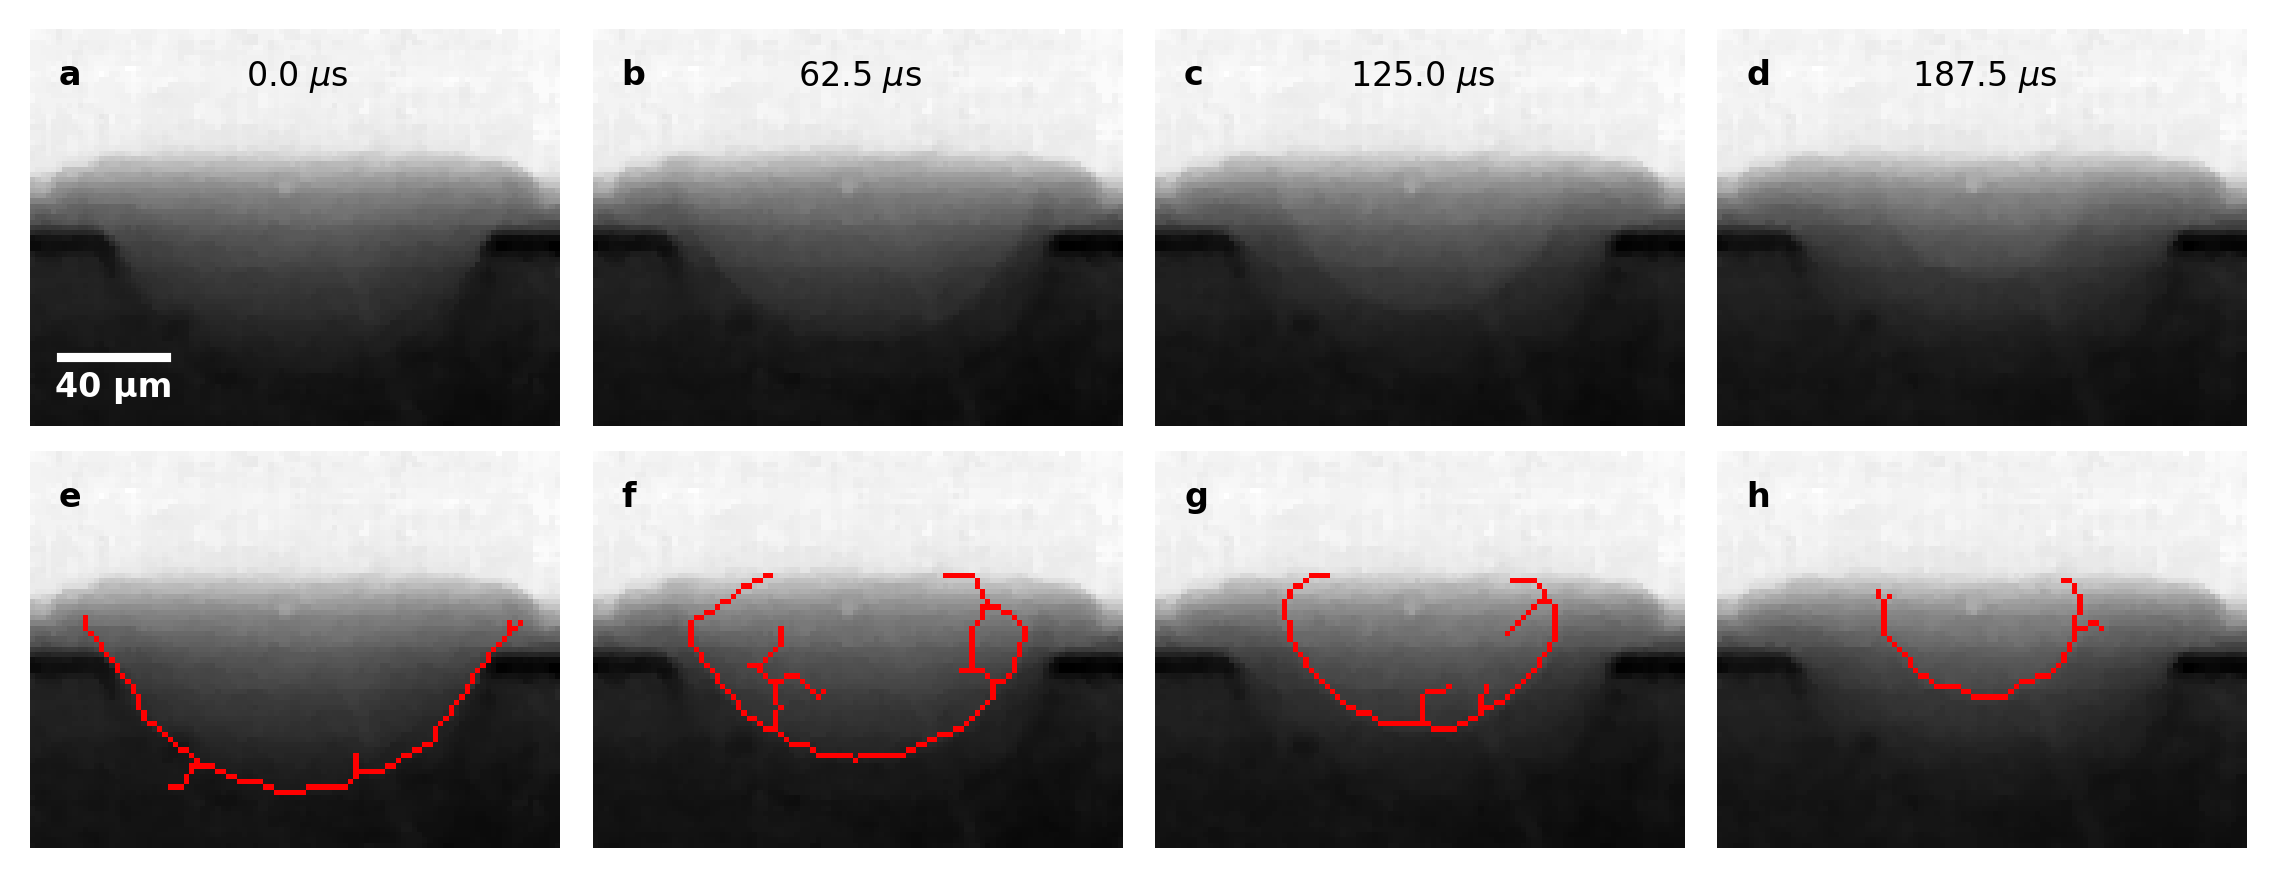
\includegraphics[width=0.9\textwidth]{figures/04/03-skel-overlay.png}
    \caption{
        \small\setstretch{1}
        (a - d) Subset of radiography sequence, showing the solid-liquid
        interface receding throughout the experiment.
        (e - f) Skeletonized regions overlaid in red on subset of
        radiography sequence, showing the as-detected position of the
        solid-liquid interface throughout the experiment.
    }
    \label{fig/skel-overlay}
\end{figure}

\subsubsection{Simulated AM Manual Measurements}
% -------------------------------------------------------------------------
The position of the detected S-L interfaces was compared to manual
measurements to assess the performance of the detection procedure.
The Python package \textit{napari} enables a graphic user interface (GUI)
window to annotate multi-dimensional images, which was used to manually
track the interfaces. The sequence of radiographs was opened in a
\textit{napari} series of frames segmented from the raw image.
A \textit{napari} points layer was also added to the window. This allowed a
user to annotate the images with a point denoting the bottom of the interface
for each image. This manual annotation was performed three times such that
the variance of individual manual measurements could be analyzed and
compared to the mean manual measurement along with the detected S-L
interface locations.


% Under Methods section
% --------------------------------------------------
\subsubsection{Al-Si Rapid Solidification}
% --------------------------------------------------
To accurately model Al-Si solidification, solidification velocity must
first be measured from experiments. Solidification was monitored in situ
with a Dynamic Transmission Electron Microscope (DTEM).
A thin film of Al-3 wt.\% Si is deposited on a silicon nitride surface with a
thickness of approximately 100 nm.
A laser melts the Al-Si film and after a 20 µs delay, an electron beam
pulsing at 2.5 µs intervals is transmitted through the sample. The
resulting beam is rastered across a detector, which captures nine frames
of the solidification at 120x
magnification in a single image (\ref{fig/raw-false-color}).
An automated
identification procedure was developed to calculate the solidification
velocity by identifying the rapidly solidifying melt pool in each frame,
fitting an ellipse to each of the melt pools,
and analyzing the change in size of the ellipses. This procedure consists of
a series of Python functions, mostly implemented using a set of
packages similar to the packages used in the AM simulator procedure:
\textit{imageio}, \textit{NumPy}, \textit{scikit-image},
\textit{matplotlib}, \textit{SciPy}.
The functions were executed in \textit{Jupyter}
notebooks to yield incremental results at each step for three separate DTEM
images depicting rapid solidification of Al-3 wt.\% Si.

\begin{figure}[ht]
    \centering
    \includegraphics[width=0.9\textwidth]{figures/04/04-raw-false-color.png}
    \caption{
        \small\setstretch{1}
        (a) Dynamic transmission electron microscope (DTEM) image showing
        nine frames of a rapidly solidifying Al-3 Si sample with a 20 µs
        delay and 2.5 µs capture interval. The chronology of the experiment
        starts with the lower right image, moves up the right column, down
        the center column, and finally up the left column to end at the top
        left image.
        (b) The same image with false color highlighting intensity
        differences across the image.
    }
    \label{fig/raw-false-color}
\end{figure}

\subsubsection{Rapid Solidification Detection Procedure}
% --------------------------------------------------
The detection procedure consists of four parts:
preprocessing, morphologic operations, ellipse fitting, and analysis. In
the preprocessing routine, the DTEM image is separated into nine frames by
performing a lower minimum threshold to create a binary image. The binary
image contains masks of the nine elliptical frames, which are labeled
according to connected pixel region in the image using a \textit{scikit-image}.
The labeled image is passed to the \textit{scikit-image} function
\textit{measure.regionprops}, which provides information necessary to crop
each of the nine frames and center them into nine separate images of matching
size. For each of
these separated frames, a pseudo-flat-field image is created by smoothing
the image with a large Gaussian filter and replacing the background pixels
(beyond the elliptical frame) with the mean intensity of the image
(\ref{fig/raw-flatfield}). Each resulting pseudo-flat-field image is
used to normalize each frame, smoothing out localized intensity fluctuations.
This pseudo-flat-field correction is performed for each of the nine frames
(\ref{fig/raw-rescaled}).

\begin{figure}[ht]
    \centering
    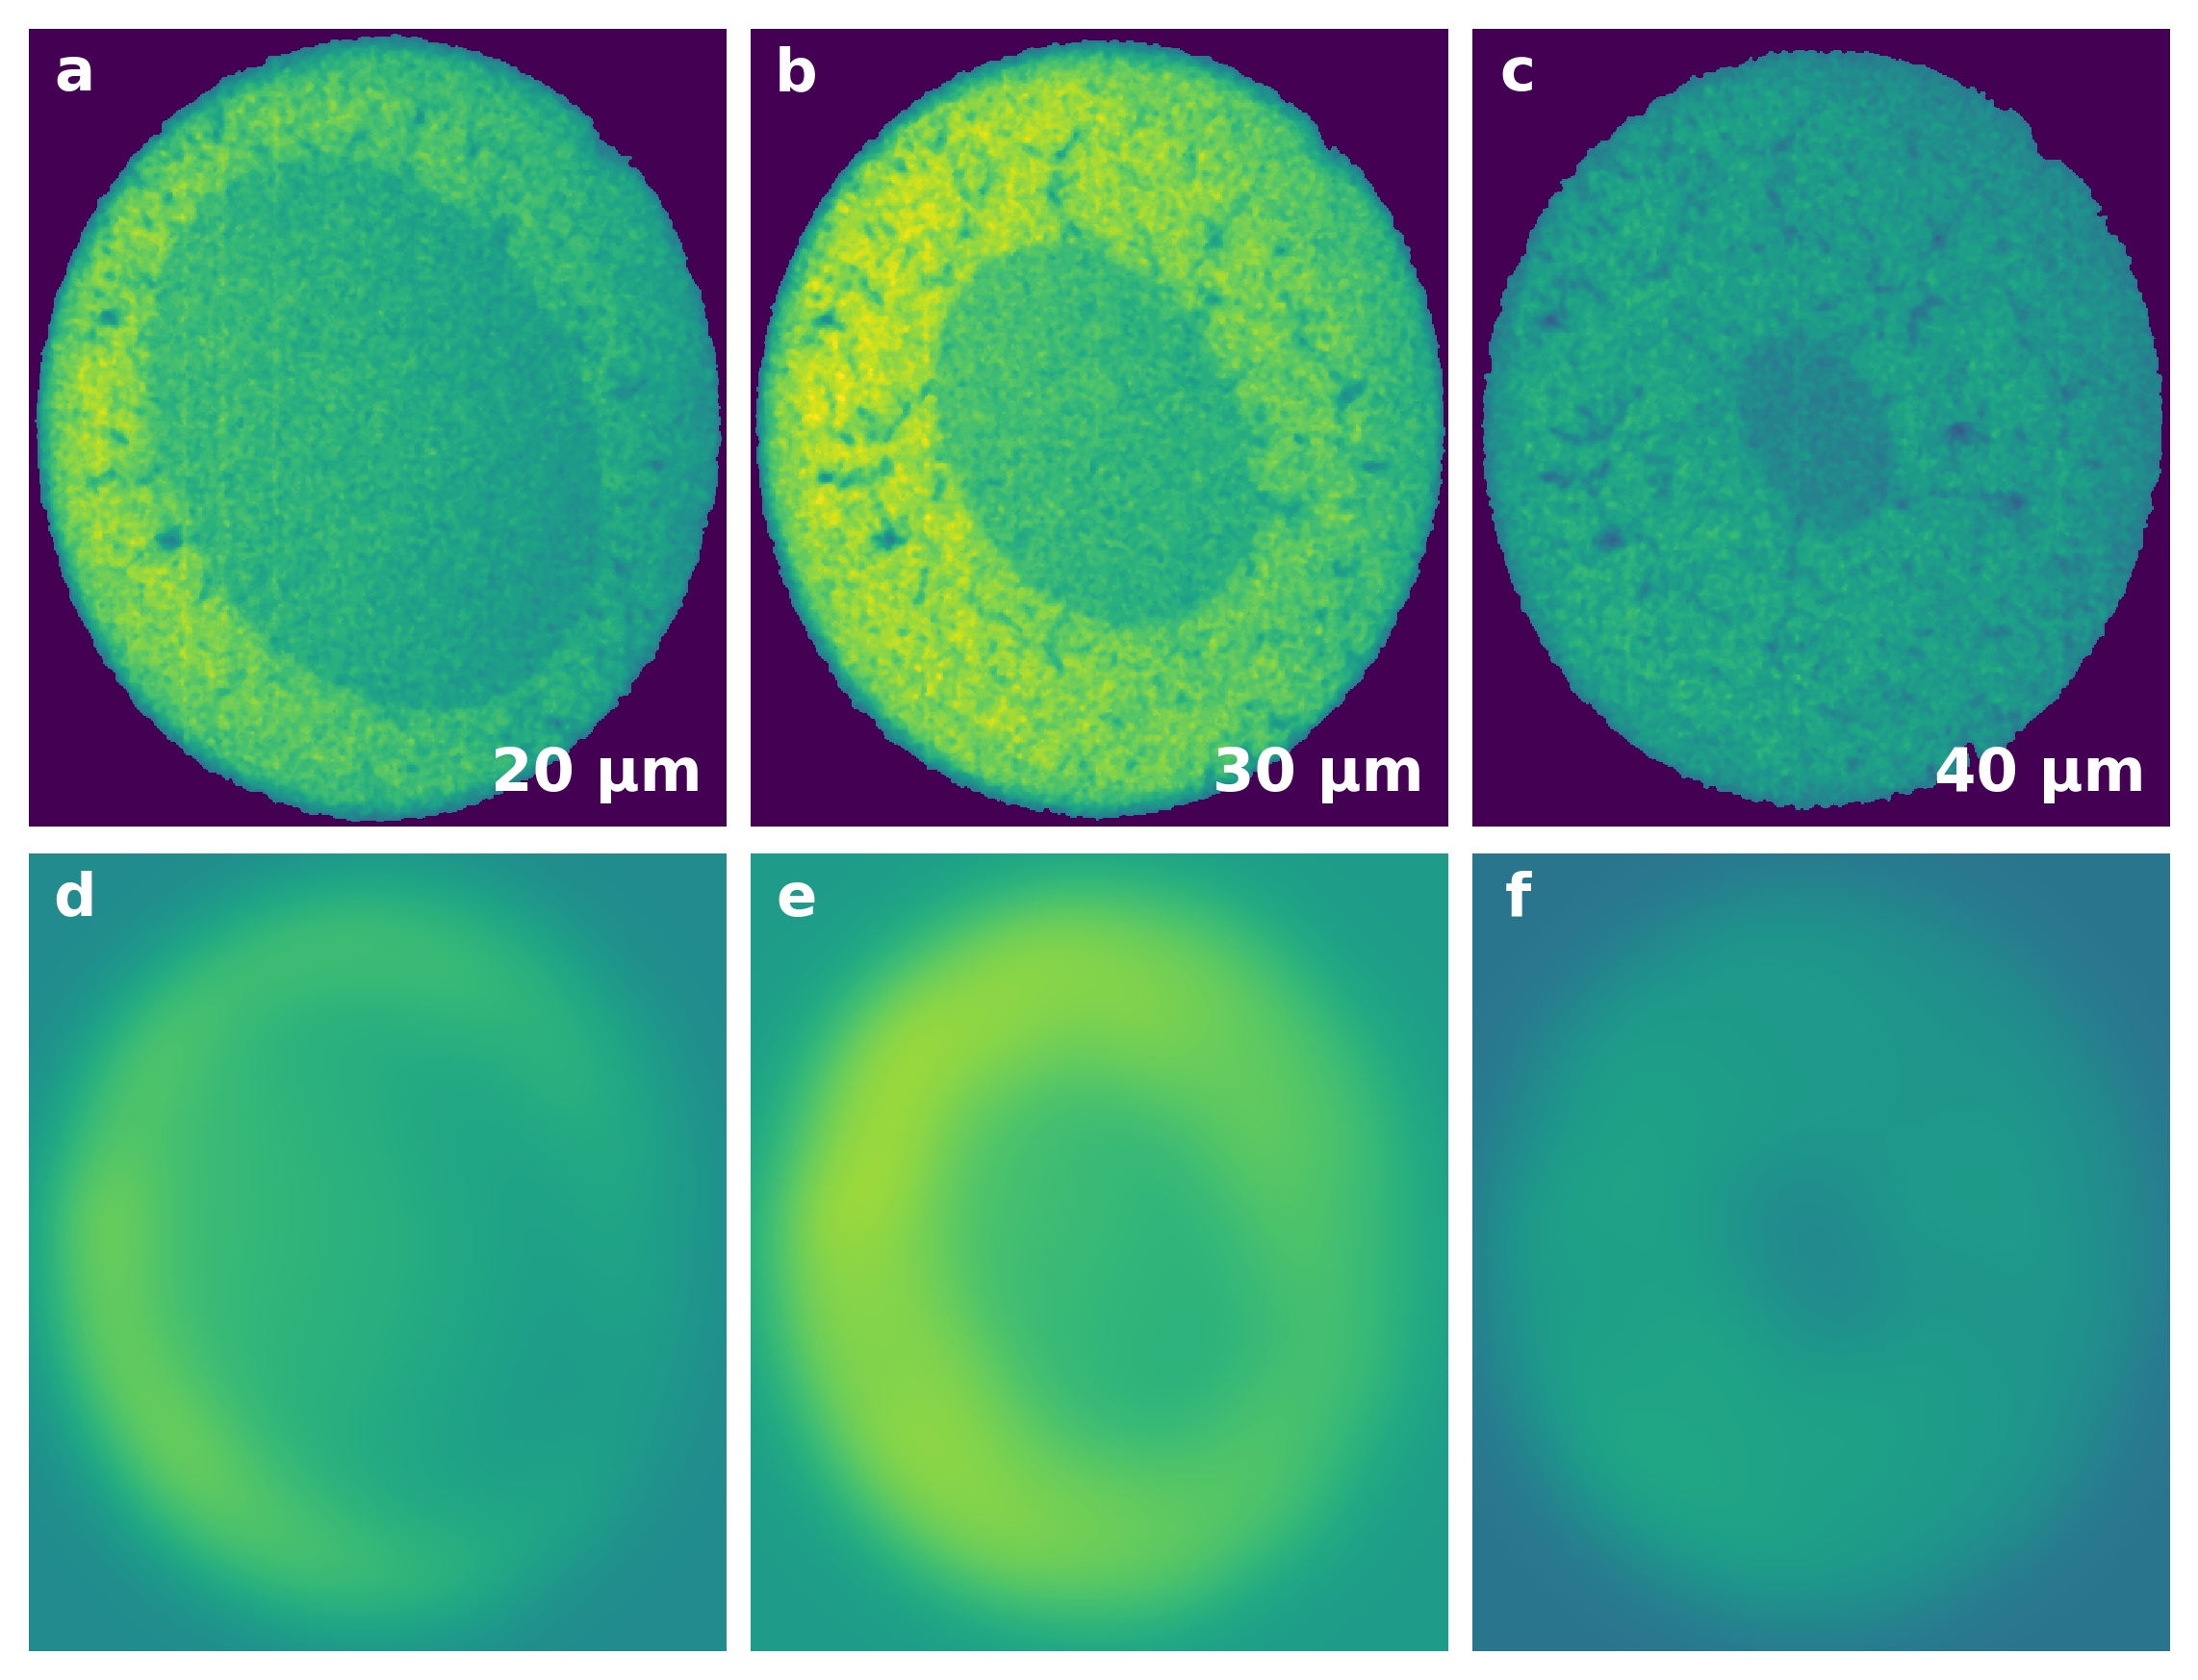
\includegraphics[width=0.6\textwidth]{figures/04/05-raw-flatfield.png}
    \caption{
        \small\setstretch{1}
        (a - c) Subset of frames with intensity unchanged following
        extraction from full DTEM image. Frames correspond to 20 µs, 30 µs,
        and 40 µs after the laser melted the sample.
        (d - f) Pseudo flat-field images created with large-sigma Gaussian
        filter and mean-filled background.
        Created from corresponding frames (a - c).
    }
    \label{fig/raw-flatfield}
\end{figure}

\begin{figure}[h]
    \centering
    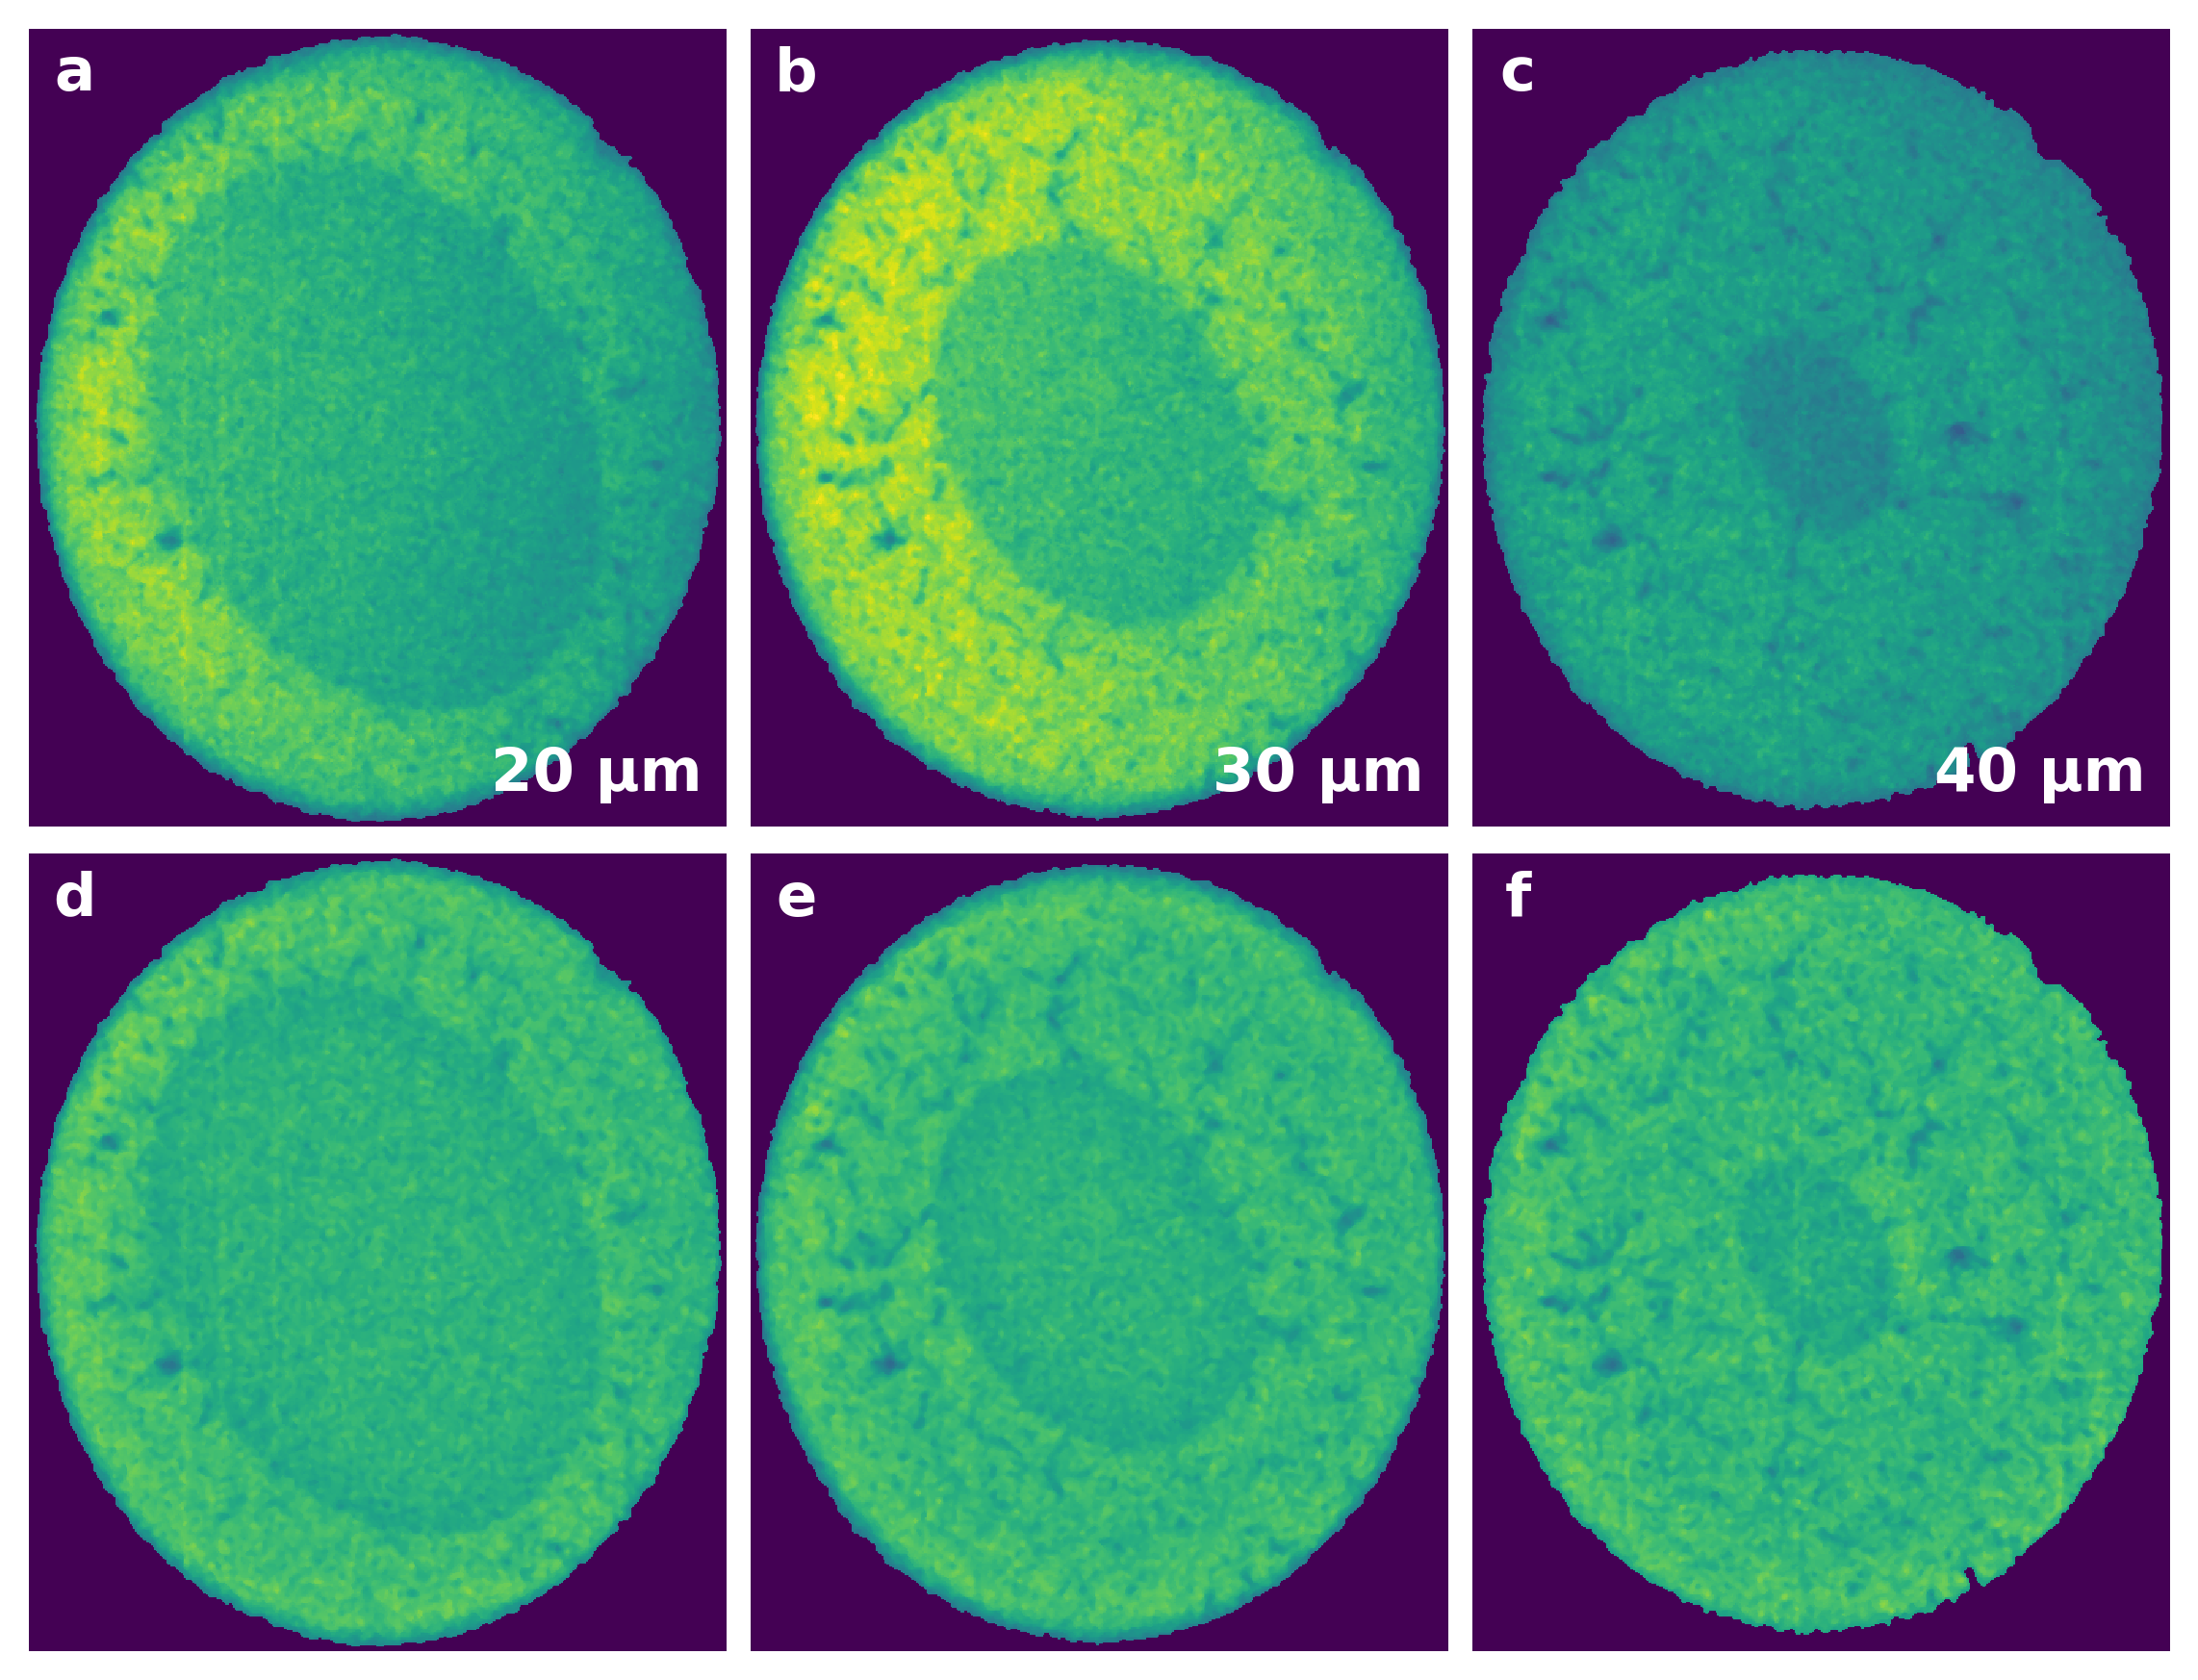
\includegraphics[width=0.6\textwidth]{figures/04/06-raw-rescaled.png}
    \caption{
        \small\setstretch{1}
        Comparison between raw DTEM frames and intensity-rescaled frames
        following pseudo-flat-field correction.
        (a - c) Subset of frames with intensity unchanged following
        extraction from full DTEM image. Frames correspond to 20 µs, 30 µs,
        and 40 µs after the laser melted the sample.
        (d - f) Subset of frames following pseudo flat-field images created
        with large-sigma Gaussian filter and mean-filled background.
        Created from corresponding frames as (a - c) and pseudo flat-field
        images (\ref{fig/raw-flatfield}.d - f).
    }
    \label{fig/raw-rescaled}
\end{figure}

Following the pseudo-flat-field correction, the rescaled frames are then
subjected to the morphologic operation stage of the procedure. An upper
minimum threshold is used to create a binary image (\ref{fig/morpho}.a),
on which morphologic opening is performed to sever connections across the melt
pool. With regions disconnected, regions smaller than the mean region size
are removed from the binary image (\ref{fig/morpho}.b), then the image
is inverted and regions at the border of the image are removed
(\ref{fig/morpho}.c). At this point, the largest region is selected
(\ref{fig/morpho}.d) and morphologic closing is performed to close any
remaining gaps across the area corresponding to the S-L interface
(\ref{fig/morpho}.e). Finally, all the holes inside the
remaining region are filled, to create a single, roughly elliptical shape
(\ref{fig/morpho}.f).

\begin{figure}[ht]
    \centering
    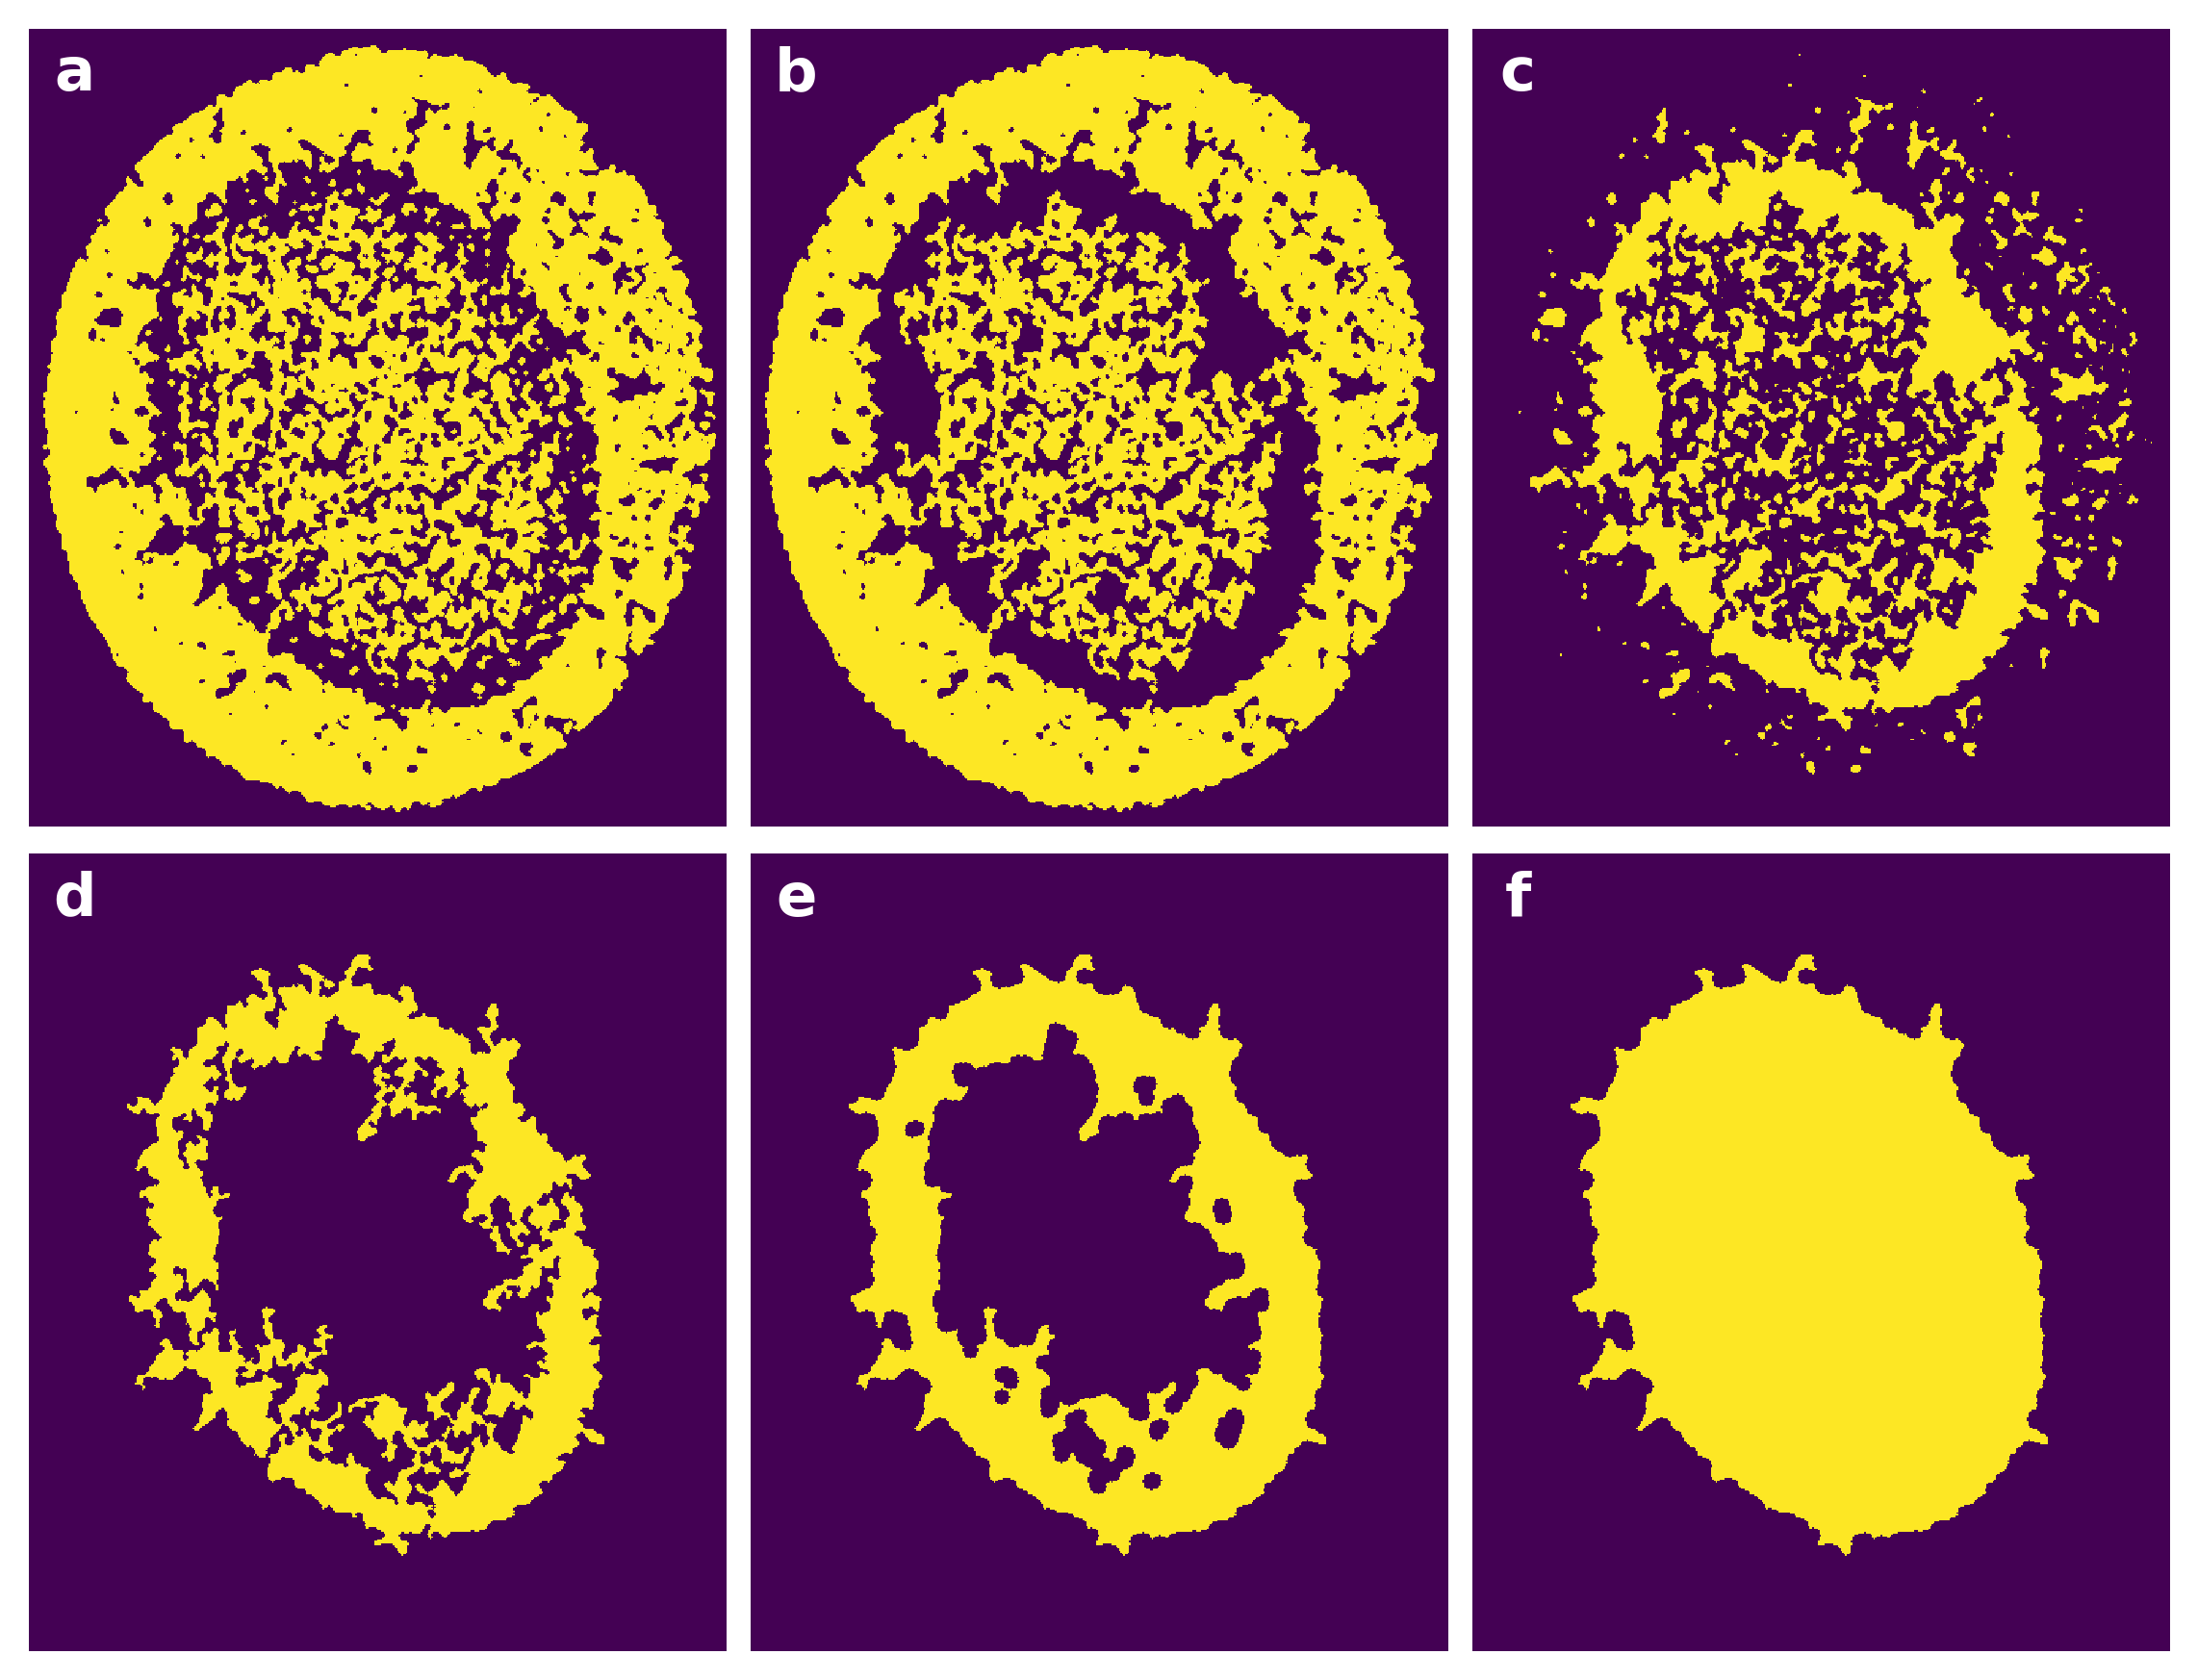
\includegraphics[width=0.6\textwidth]{figures/04/07-morpho.png}
    \caption{
        \small\setstretch{1}
        Series of morphological operations to automatically mask the
        liquid region of each solidifying frame from the DTEM image.
        (a) Upper minimum threshold of 20 µs frame
        (\ref{fig/raw-rescaled}.d).
        (b) Result of morphological opening of (a) to severe small
        connections across the solid-liquid interface followed by filtering
        of regions smaller than the mean area of all the regions present.
        (c) Inversion of b followed by removal of regions connected to the
        border.
        (d) Selection of region in (c) with largest area.
        (e) Morphological closing of (c) to connect small gaps across the
        solid-liquid interface that were not disconnected in the opening in (b).
        (f) Filling of all holes to create the final identified region.
    }
    \label{fig/morpho}
\end{figure}

This routine is performed for each frame, resulting in nine roughly
elliptical identified regions. These regions contain the melt pools,
though the masks contain artifacts branching off from the elliptical melt
pools that correspond to darker features around the edge of the true melt
pools (\ref{fig/rescaled-filled}).

\begin{figure}[ht]
    \centering
    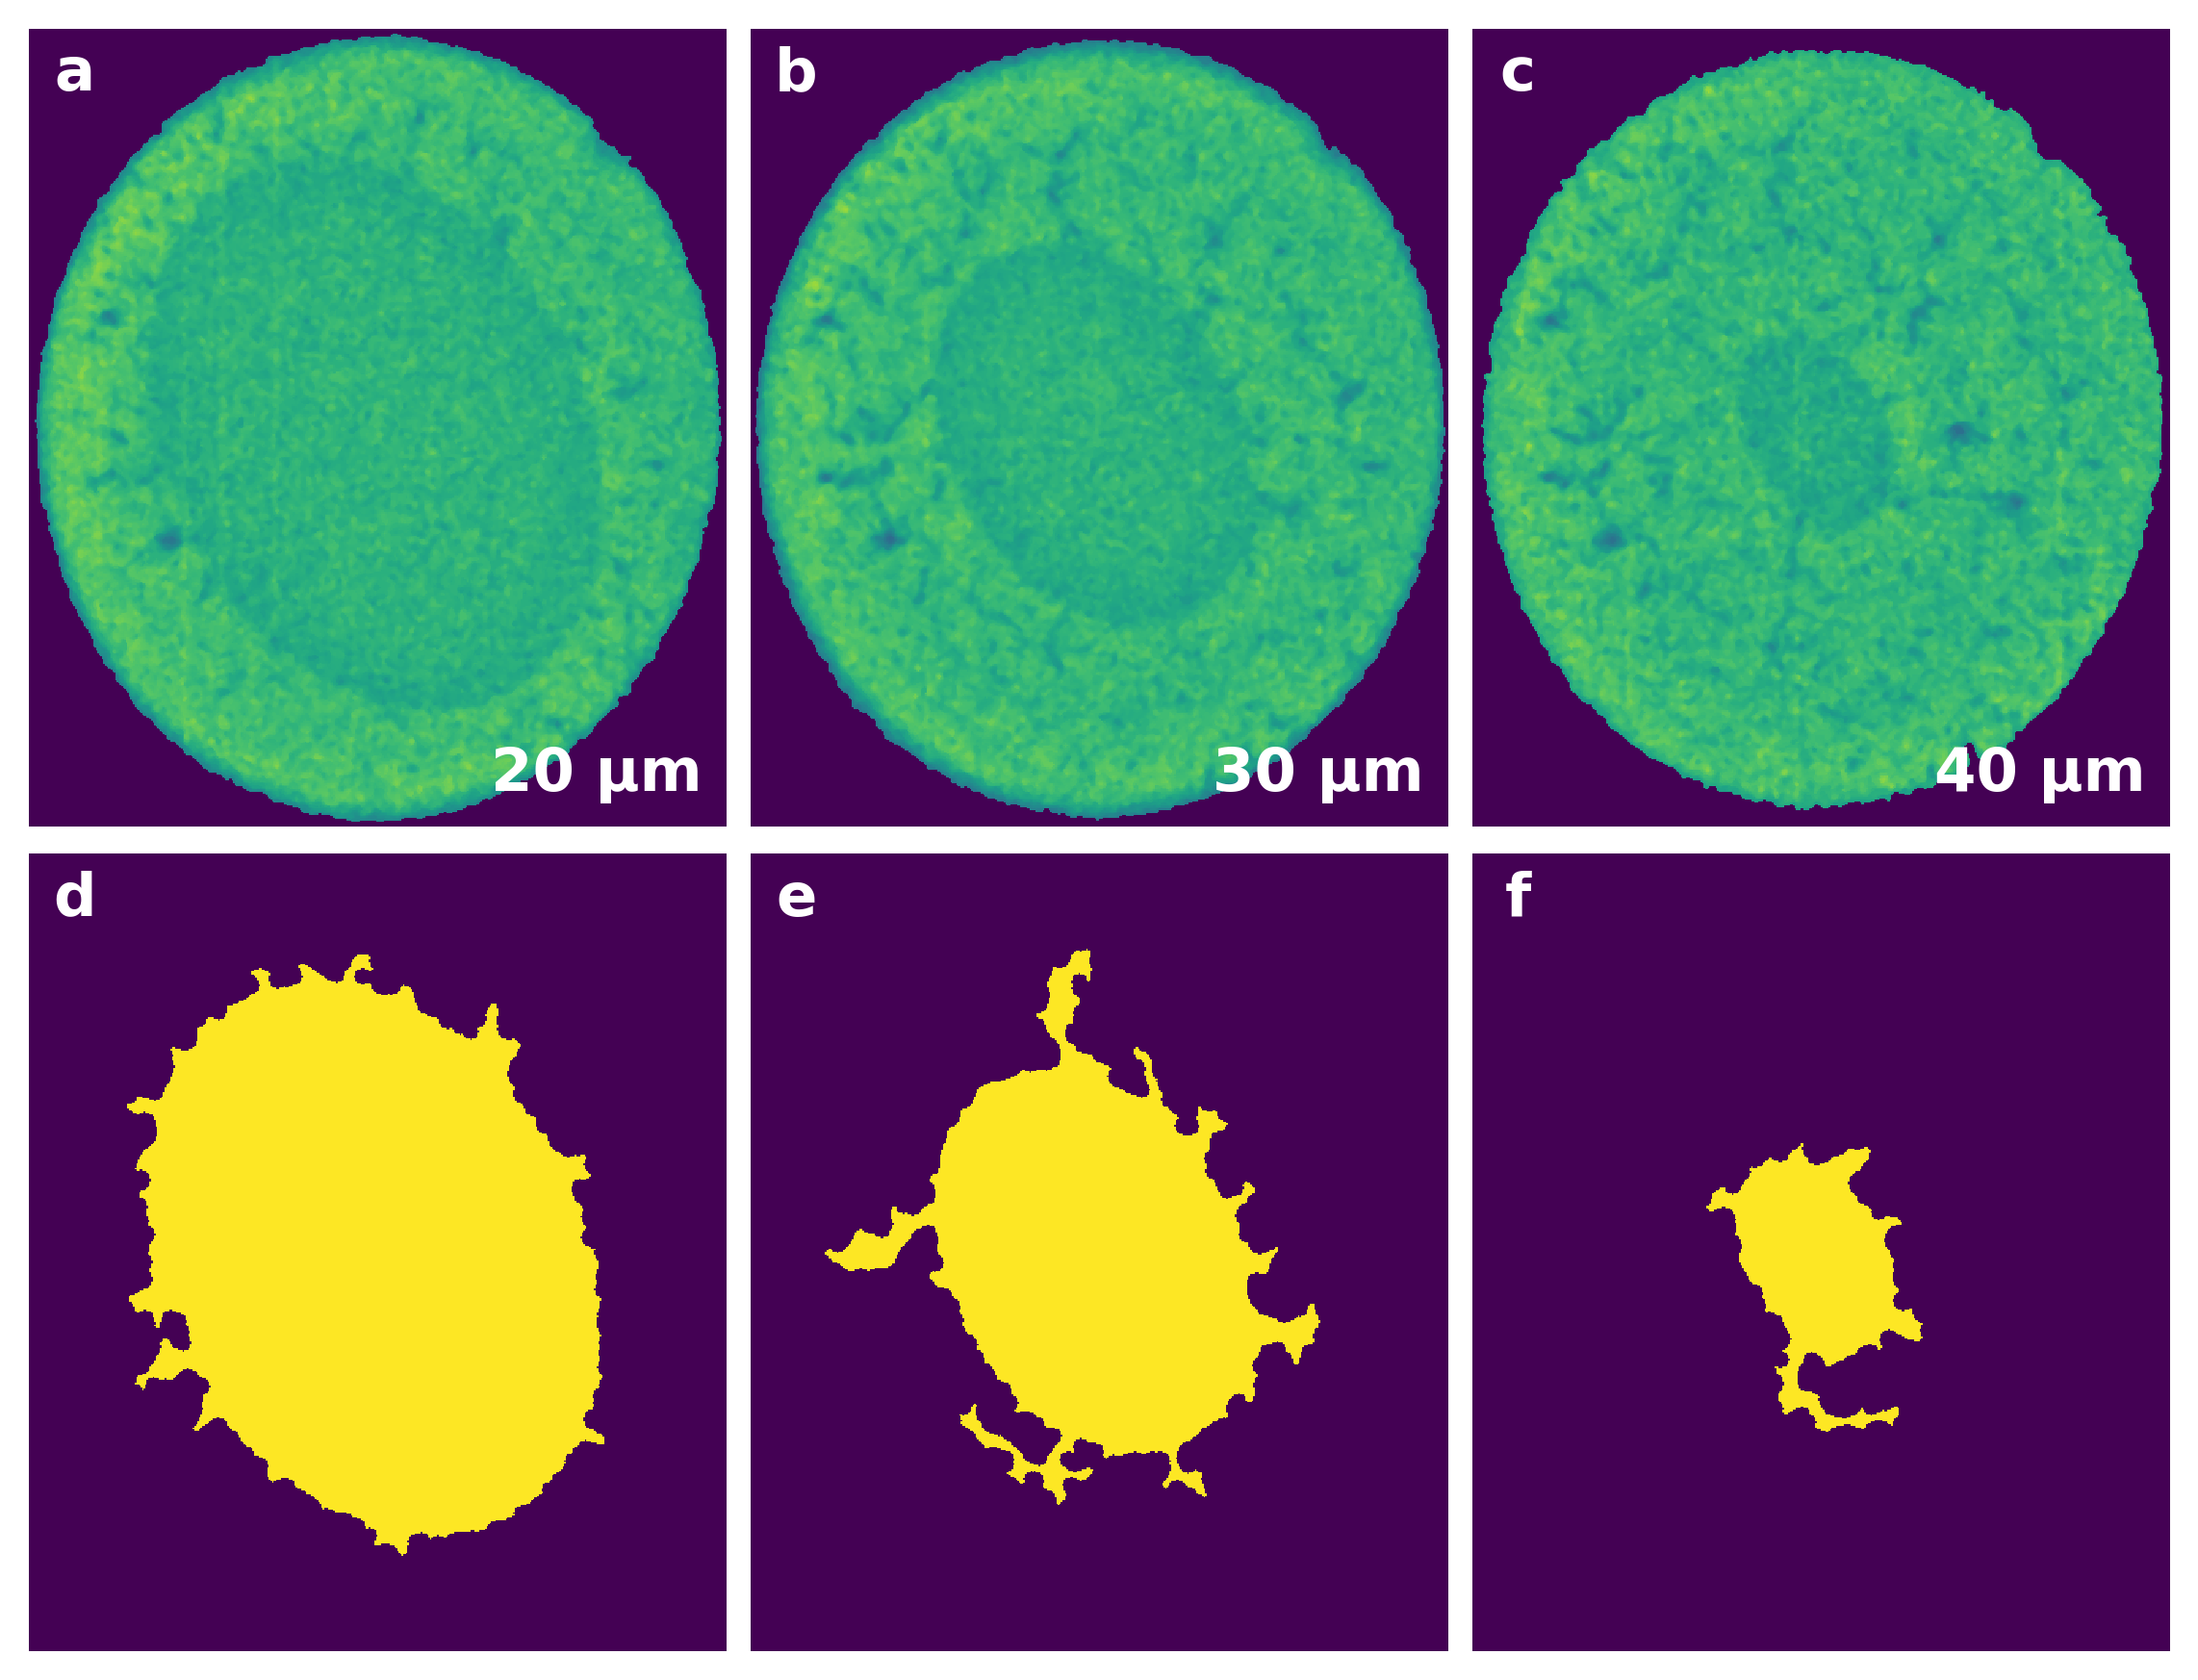
\includegraphics[width=0.6\textwidth]{figures/04/08-rescaled-filled.png}
    \caption{
        \small\setstretch{1}
        (a - c) Subset of normalized frames depicting Al-Si solidification
        20 µs, 30 µs, and 40 µs after the laser melted the sample.
        (d - f) Roughly elliptical identified regions containing the melt
        pools resulting from the series of morphologic operations
        (\ref{fig/morpho}.a - f)
        applied to each frame.
    }
    \label{fig/rescaled-filled}
\end{figure}

The ellipse fitting stage of the routine takes the identified region for
each frame and fits an ellipse to the region. An ellipse with the same
second moment as the identified region is calculated with the
\textit{scikit-image}
function \textit{measure.regionprops} as a first approximation fit. This
ellipse is rasterized onto an image of the same size as the
and at the same centroid as the identified region.
Both the fitted ellipse and the identified region are represented as binary
images with pixel intensities of either one or zero, so the mismatch
between the two images can be represented by the sum of the pixels shared
between the two images.
True fit pixels represent the pixels valued one in both images.
Misfit pixels represent the pixels valued valued zero in the
identified region but valued one in the fitted ellipse image.
Unfit pixels represent the pixels valued one in the identified regions but
valued zero in the fitted ellipse image.
Each of these types of pixels can be visualized by overlaying the fitted
ellipse image on the identified regions
and assigning different colors to different pixel types
(\ref{fig/rescaled-nonoptim}).

\begin{figure}[ht]
    \centering
    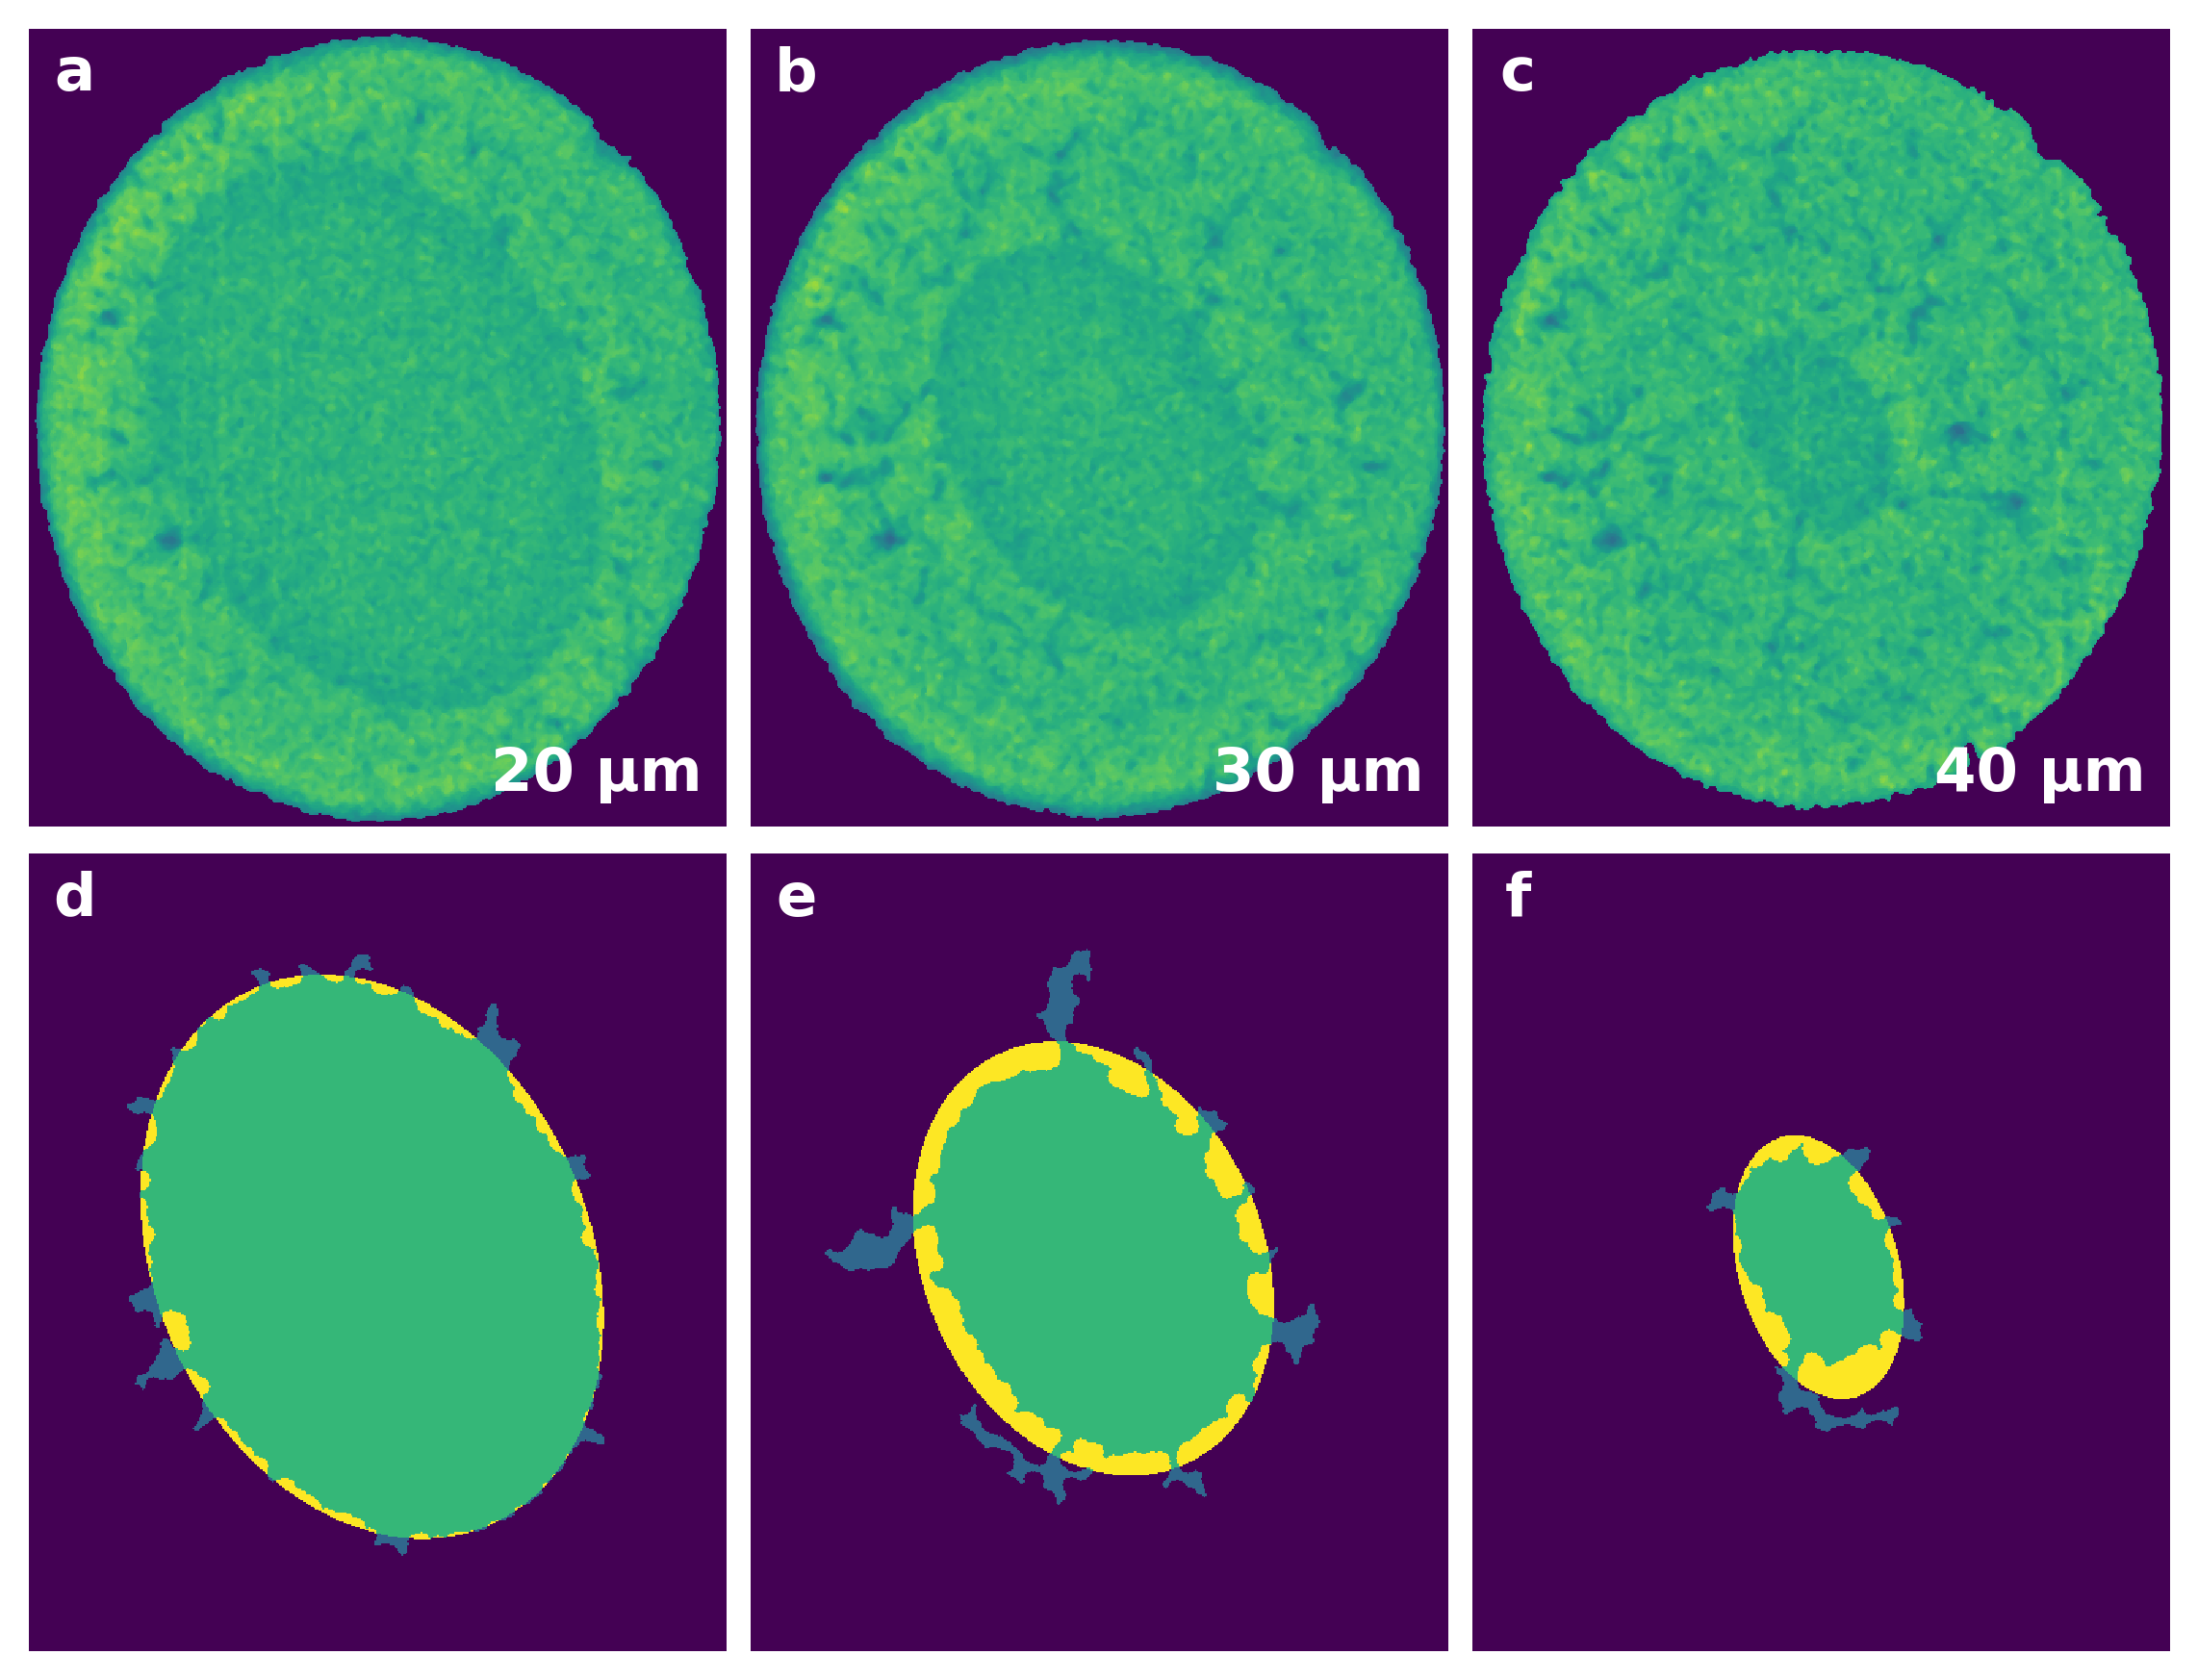
\includegraphics[width=0.6\textwidth]{figures/04/09-rescaled-nonoptim-fit.png}
    \caption{
        \small\setstretch{1}
        (a - c) Subset of normalized frames depicting Al-Si solidification
        20 µs, 30 µs, and 40 µs after the laser melted the sample.
        (d - f) Identified regions overlaid with fitted ellipses generated by
        finding ellipse parameters that match the centroid and second
        moment of the identified regions. The color of the pixels show the
        extent to which the fit matches the identified region.
        True fit pixels are within both the identified region and
        the ellipse (green), misfit pixels are beyond the identified
        region but still within the ellipse (yellow), and unfit pixels are
        beyond both the identified region and the ellipse (blue).
    }
    \label{fig/rescaled-nonoptim}
\end{figure}

The ellipse of equal second moment from \textit{scikit-image}
(\ref{fig/rescaled-nonoptim}) is used
as a starting point for fit optimization. The parameters defining the
ellipse (centroid x-coordinate, centroid y-coordinate, minor radius, major
radius, and orientation) are optimized using the downhill simplex
algorithm \cite{Nelder1965} implemented in \textit{SciPy} as the function
\textit{optimize.fmin}.
This function works by minimizing the value returned by a custom cost
function (Equation \ref{eqn/cost}) for a frame with $m$ rows and $n$
columns:
\begin{equation} \label{eqn/cost}
    cost =
    - \left(
        \sum_{i = 0}^{m}\sum_{j = 0}^{n} T_{ij}
    \right)
    \left(
        \sum_{i = 0}^{m}\sum_{j = 0}^{n} T_{ij}
        + \sum_{i = 0}^{m}\sum_{j = 0}^{n} M_{ij}
        + \frac{1}{4} \sum_{i = 0}^{m}\sum_{j = 0}^{n} U_{ij}
    \right)^{-1}
\end{equation}
where
$T$ represents a true fit pixel within both the identified region and the
fitted ellipse,
$M$ represents a misfit pixel beyond the identified region but within
the fitted ellipse, and
$U$ represents an unfit pixel beyond the identified region and the
fitted ellipse.
Including the sum of true fit pixels in the numerator and denominator
of the cost function means that a perfect fit would be a cost value of -1.
The addition of the sum of the misfit and unfit pixels in
the denominator decreases the cost value from -1 for additional pixels
that are mismatched between the fitted ellipse image and the identified
region. Since these terms are added to the sum of true fit pixels in
the denominator, the effect of each additional mismatched pixel acts
relative to the number of true fit pixels. For a frame with
larger true fit alignment, each individual mismatched pixel
contributes less to the overall cost value than the same mismatched pixel
would contribute to a frame with a smaller true fit alignment. The ¼
factor also reduces the contribution of unfit pixels, making true fit and
misfit pixels the most important factor in the cost
function, and therefore in the optimization process as a whole.

The outputted ellipse
parameters returned from the optimization process show an improvement in
the fit represented by a decrease in the sum of misfit and unfit pixels
(\ref{fig/rescaled-optim}).
It is interesting to note that most of the
unfit pixels do not appear to be part of the melt pool, but
instead correspond to darker regions of the solidified metal.

\begin{figure}[ht]
    \centering
    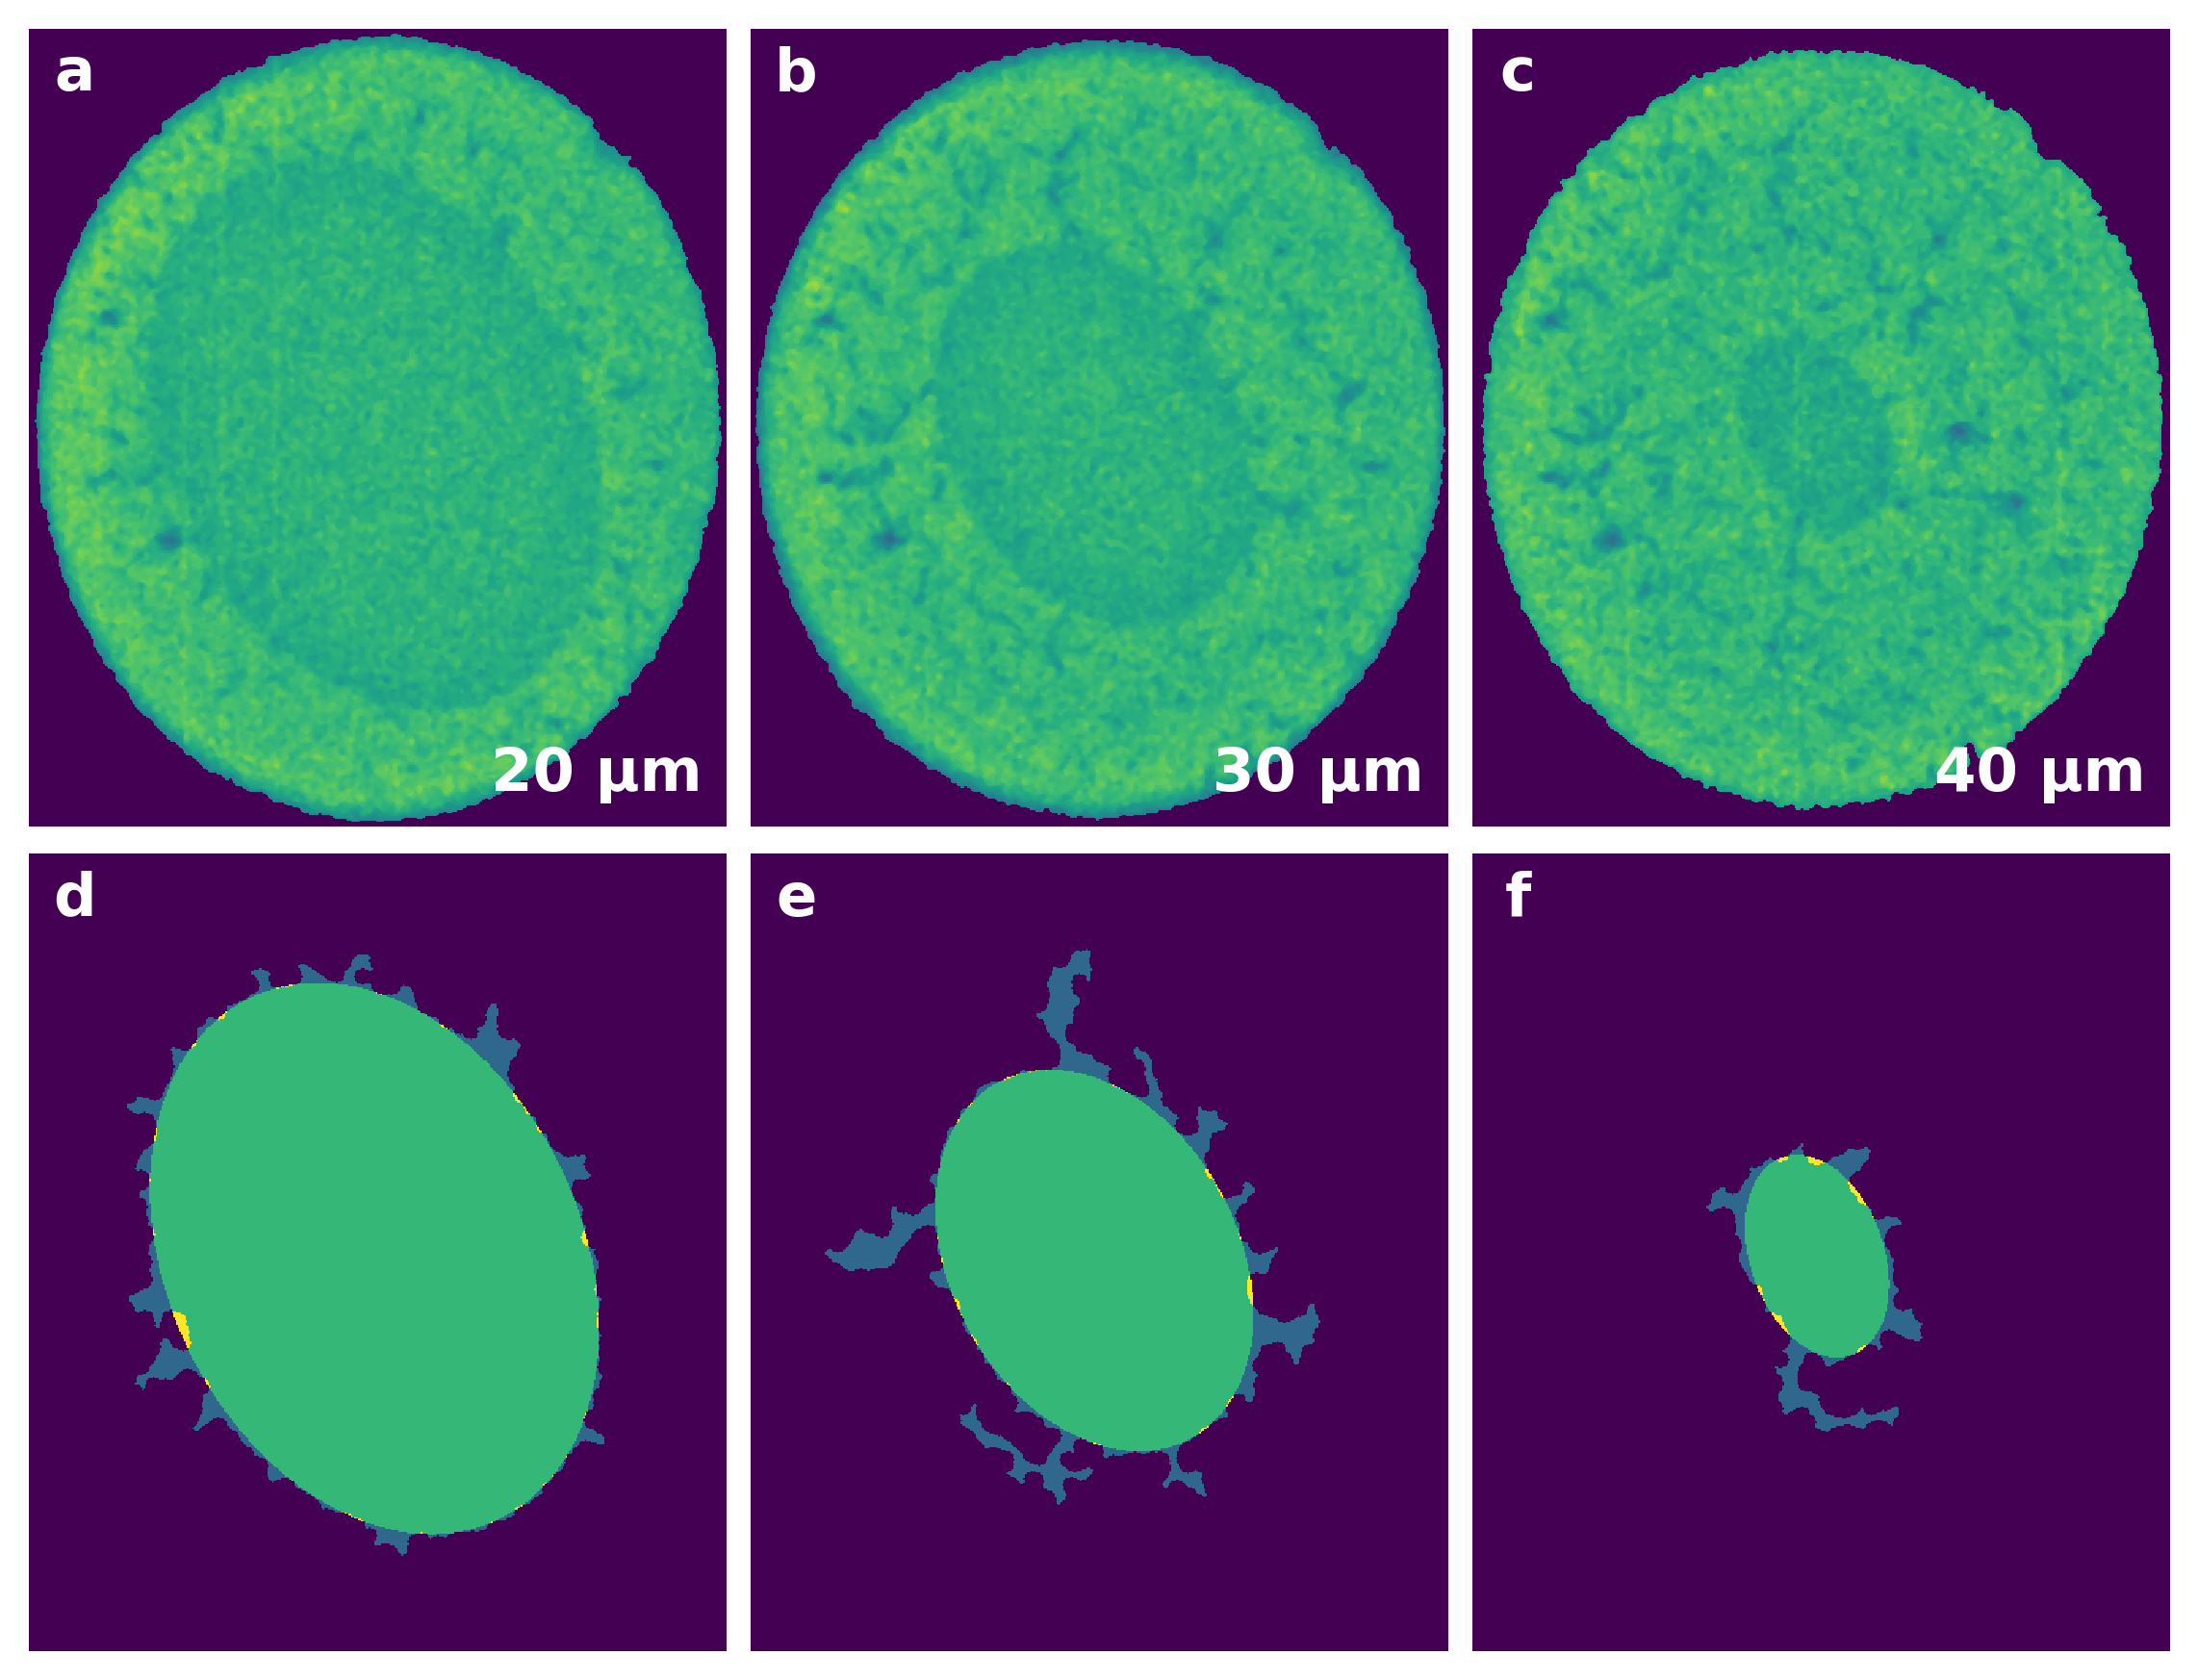
\includegraphics[width=0.75\textwidth]{figures/04/10-rescaled-optim-fit.png}
    \caption{
        \small\setstretch{1}
        (a - c) Subset of normalized frames depicting Al-Si solidification
        20 µs, 30 µs, and 40 µs after the laser melted the sample.
        (d - f) Identified regions overlaid with ellipses of optimized
        fit. Optimization maximizes true fit match (green) and minimizes
        misfit match (yellow) and unfit match (blue). The
        starting point of the optimization are the ellipses of matching
        centroid and second moment (\ref{fig/rescaled-nonoptim}. d - f).
    }
    \label{fig/rescaled-optim}
\end{figure}

The match of the optimized ellipses and the solid-liquid interface of the
experiment can be verified visually by plotting these ellipses on top of
each frame of the solidifying sample (\ref{fig/optim-ellipses}).

\begin{figure}[ht]
    \centering
    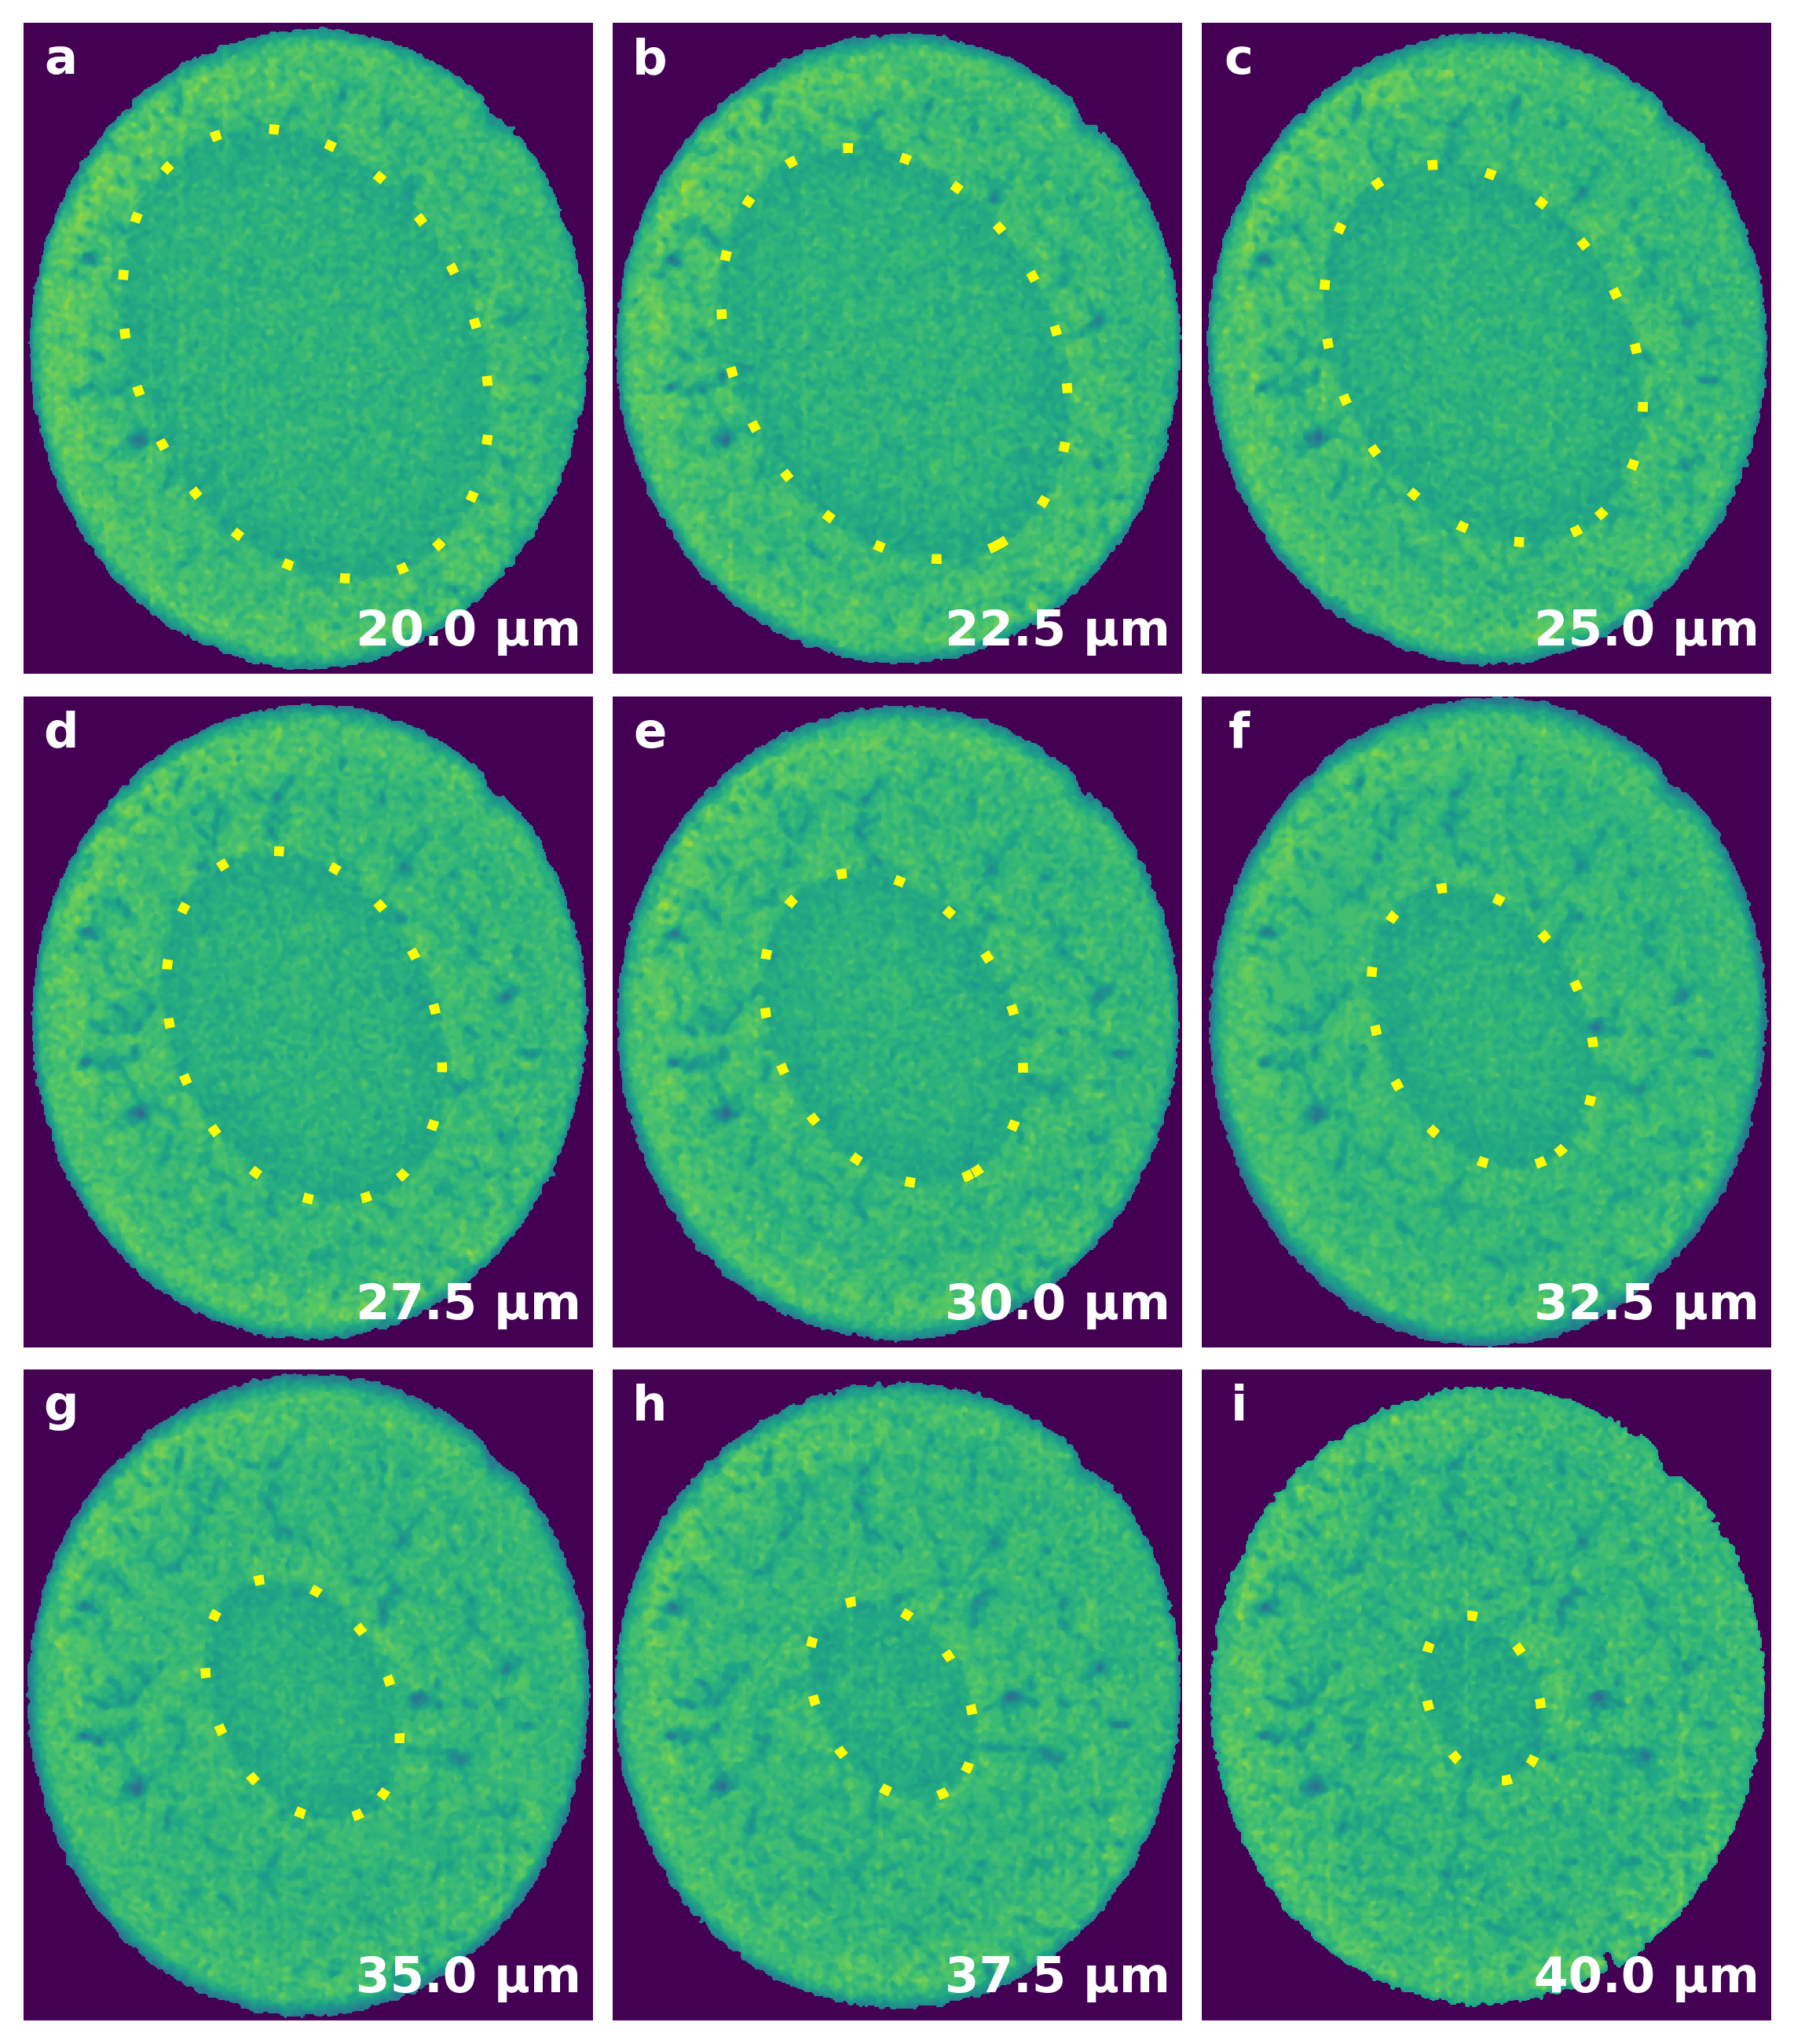
\includegraphics[width=0.6\textwidth]{figures/04/11-rescaled-optim-ellipses.png}
    \caption{
        \small\setstretch{1}
        Optimized fitted ellipses overlaid on each rescaled frame as yellow
        dashed lines.
    }
    \label{fig/optim-ellipses}
\end{figure}

\subsubsection{Rapid Solidification Manual Measurements}
% -------------------------------------------------------------------------
The size of the
optimized ellipses is compared to manual detection of the elliptical
S-L interfaces. A GUI window from the Python package \textit{napari}
was once again used for the manually measurements.
The series of frames segmented from the raw DTEM image was opened in a
\textit{napari} viewer window along with a points layer. A user placed a point
on each side of the long (major) and short (minor) axes of the melt pool.
These line segments define the size of the ellipse and was performed three
times for the DTEM image such that the variance of individual manual
measurements could also be analyzed in addition to the mean
manual measurement when assessing the performance of the detected
interface sizes.


\subsection{Results}
This section presents the detected and manually-measured solidification
velocity results for each
of the two type of experiments outlined in the previous section.

% -------------------------------------------------------------------------
\subsubsection{Simulated AM Results}
% -------------------------------------------------------------------------
The simulated AM S-L interface detection procedure and manual measurement
was applied to three separate experiments to test the performance of the
procedure.
Each experiment utilized a
different laser power to melt the sample: 104 W (20\% maximum power),
156 W (30\% maximum power), and 208 W (40\% maximum power).
In the 104 W experiment, the average velocity of the three
manually identified interfaces were calculated to be 0.058, 0.056, and 0.058
m s\textsuperscript{-1} , for a collective average velocity of 0.057
m s\textsuperscript{-1} and median of 0.057 m s\textsuperscript{-1}. The
average velocity of the detected interfaces was 0.021 m s\textsuperscript{-1},
with a median of 0.041 m s\textsuperscript{-1}.

\begin{figure}[ht]
    \centering
    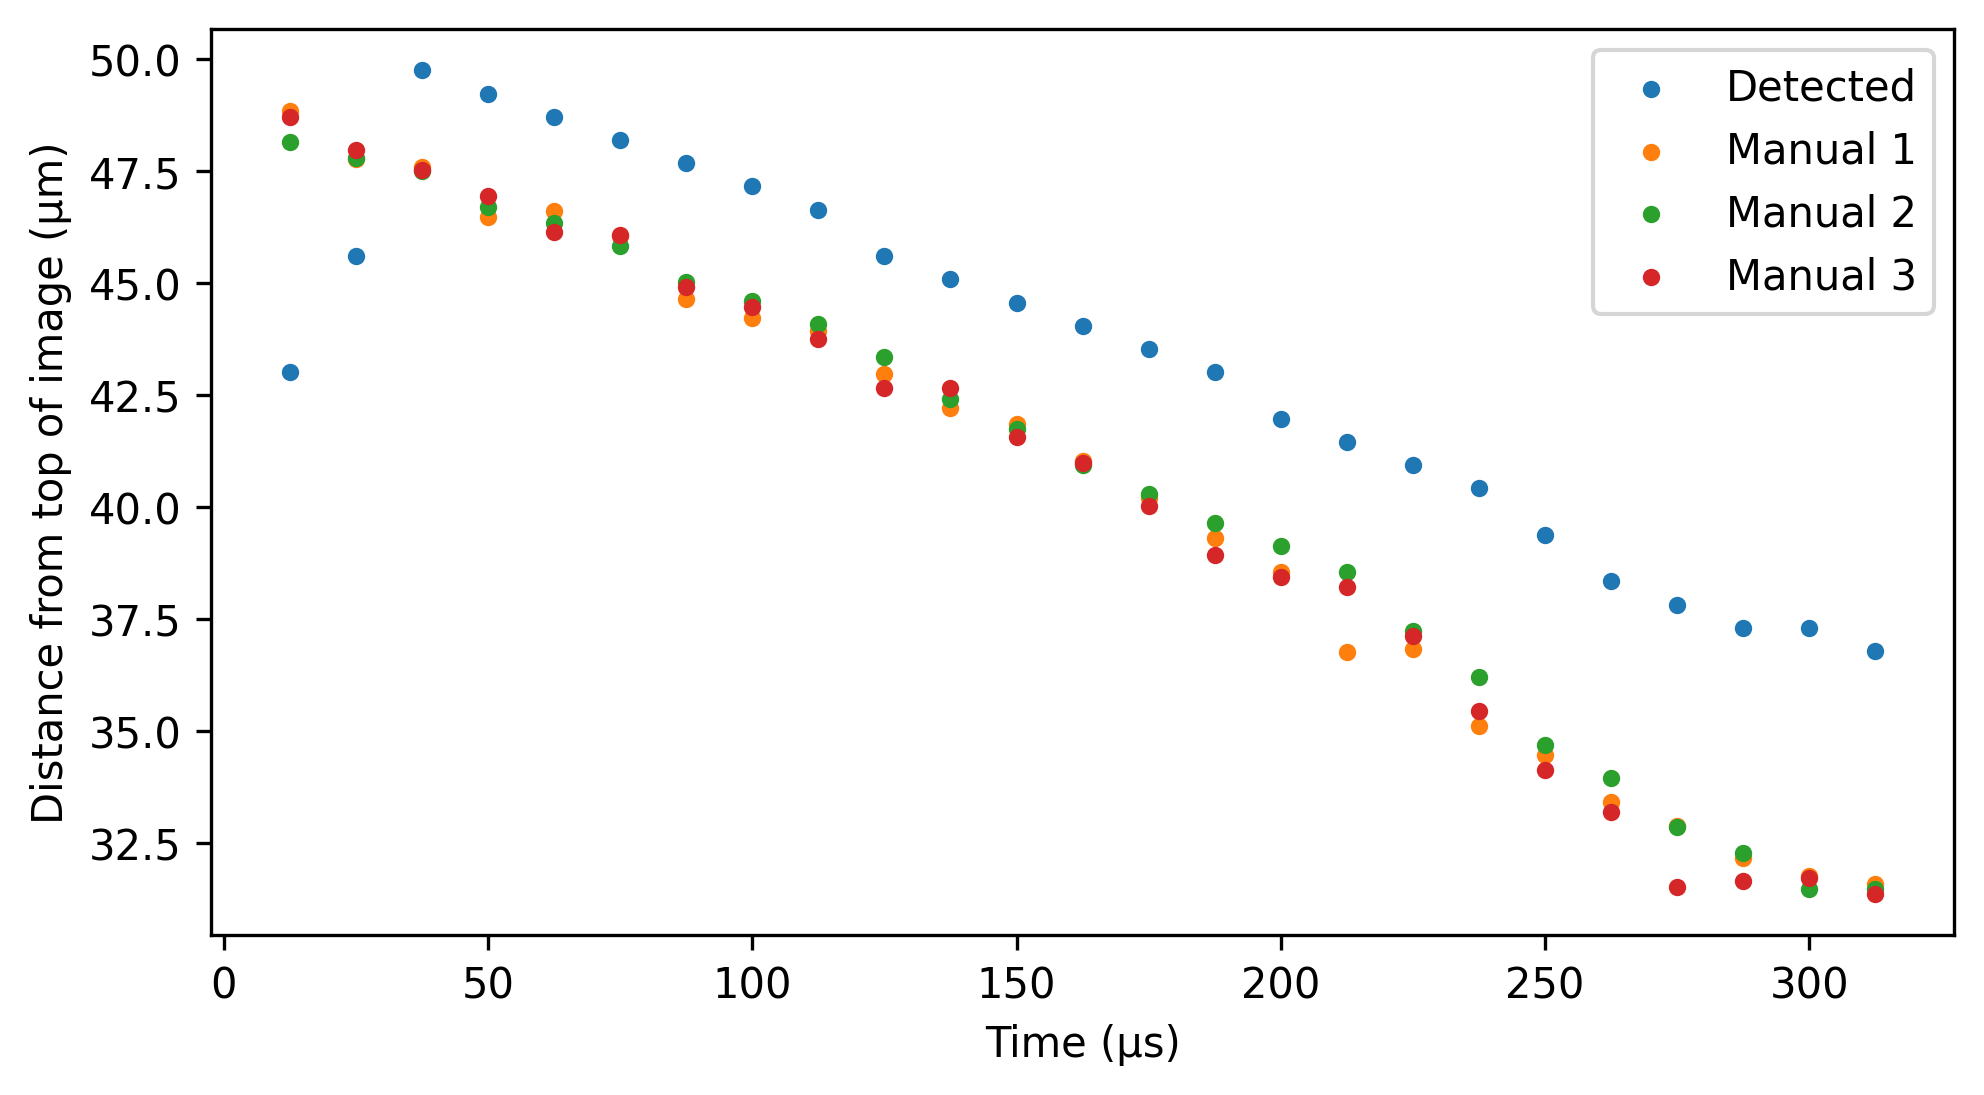
\includegraphics[width=0.75\textwidth]{figures/04/12-detected-vs-manual-1-10_shot05.png}
    \caption{
        \small\setstretch{1}
        Interfaces detected by the automated procedure (blue) compared with
        manually identified interfaces (orange, green, and red) for the
        104 W experiment. Interface location is defined by the distance from
        the bottom of the solid-liquid interface to top of the image,
        starting when the laser shuts off (t = 0 µs).
    }
    \label{fig/detected-aps-1}
\end{figure}

In the 156 W experiment, the average velocity of the three
manually identified interfaces were calculated to be 0.046, 0.046, and 0.045
m s\textsuperscript{-1}, for a collective average velocity of 0.046
m s\textsuperscript{-1} and median of 0.043 m s\textsuperscript{-1}. The
average velocity of the detected interfaces was 0.022 m s\textsuperscript{-1},
with a median of 0.041 m s\textsuperscript{-1}.

\begin{figure}[ht]
    \centering
    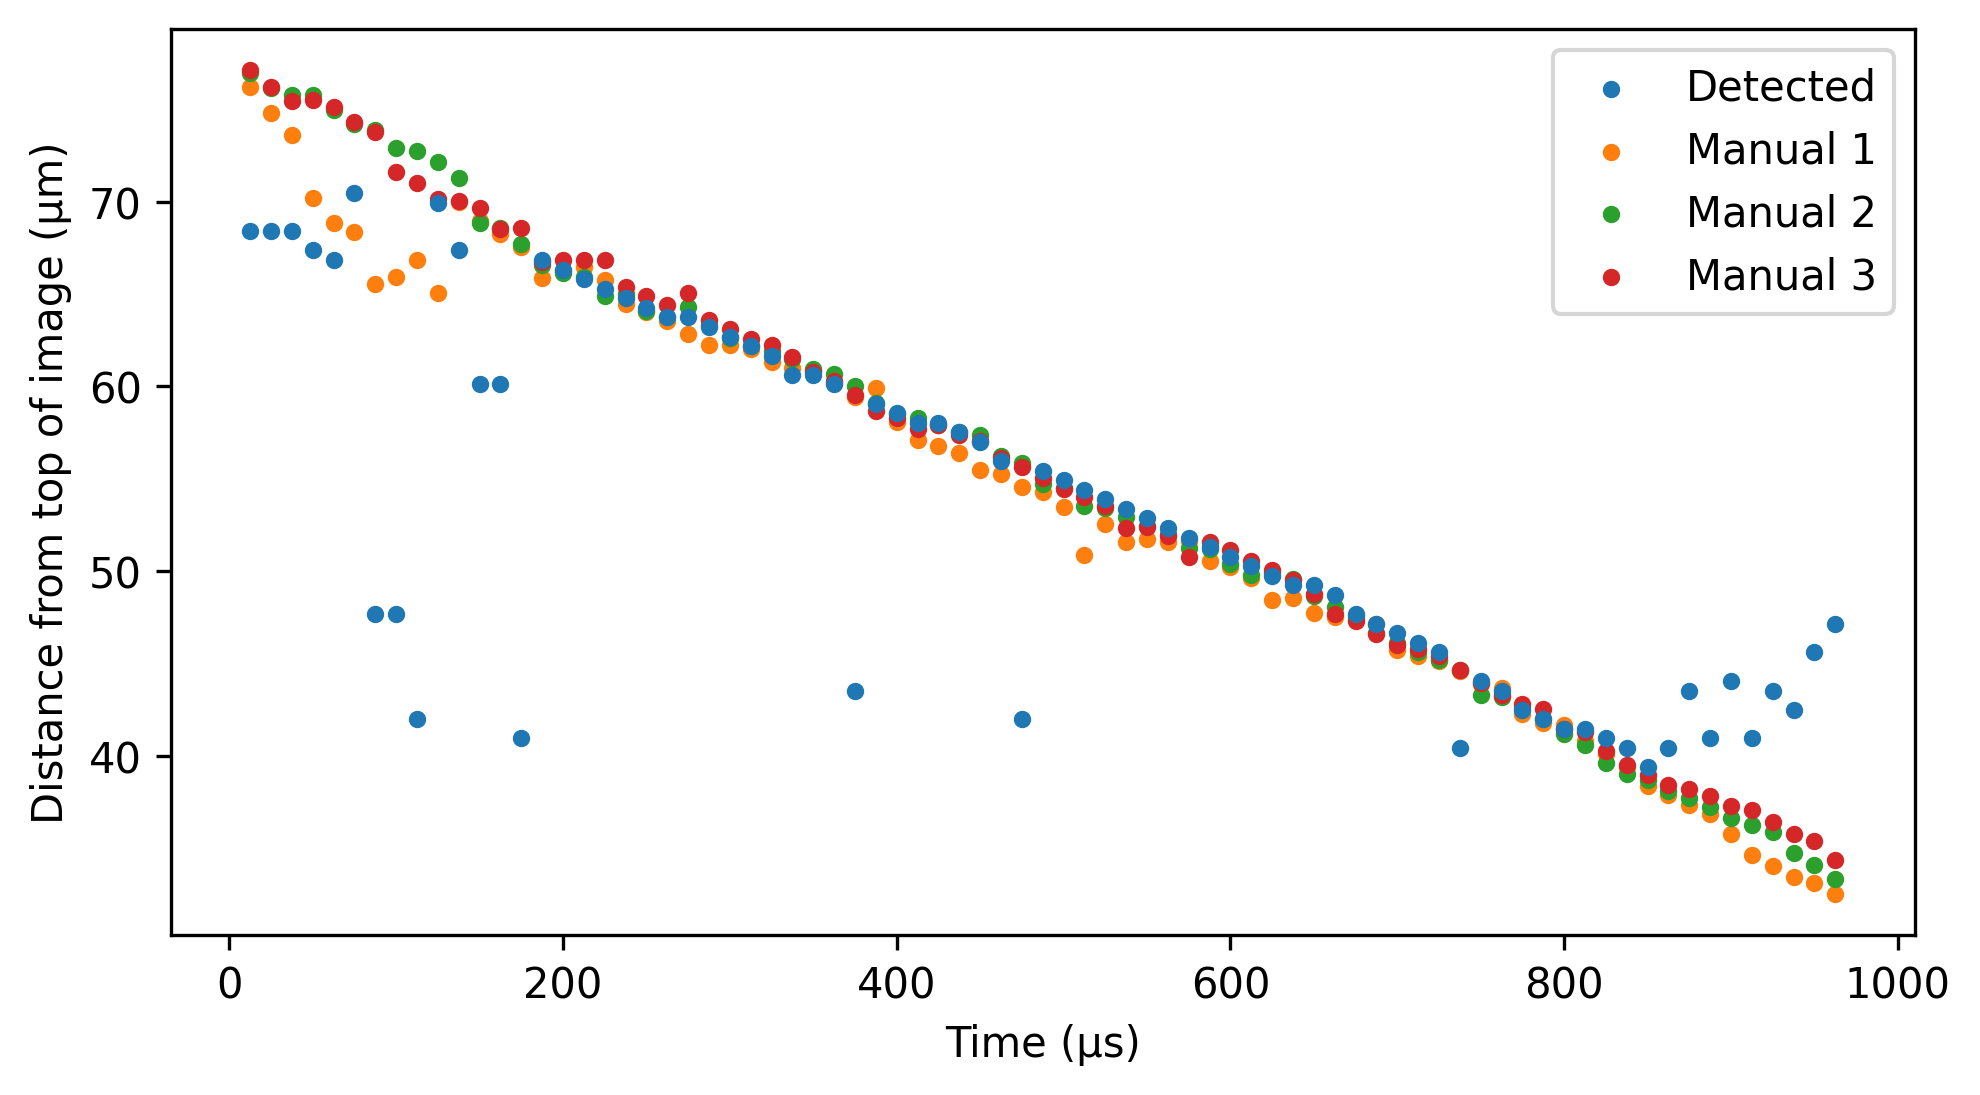
\includegraphics[width=0.75\textwidth]{figures/04/13-detected-vs-manual-2-06_shot01.png}
    \caption{
        \small\setstretch{1}
        Interfaces detected by the automated procedure (blue) compared with
        manually identified interfaces (orange, green, and red) for the
        156 W experiment. Interface location is defined by the distance from
        the bottom of the solid-liquid interface to top of the image,
        starting when the laser shuts off (t = 0 µs).
    }
    \label{fig/detected-aps-2}
\end{figure}

In the 208 W experiment, the average velocity of the three
manually identified interfaces were calculated to be 0.057, 0.058, and 0.056
m s\textsuperscript{-1}, for a collective average velocity of 0.057
m s\textsuperscript{-1} and median of 0.051 m s\textsuperscript{-1}.
The average velocity of
the detected interfaces was 0.057 m s\textsuperscript{-1}, with a median
of 0.041 m s\textsuperscript{-1}.

\begin{figure}[ht]
    \centering
    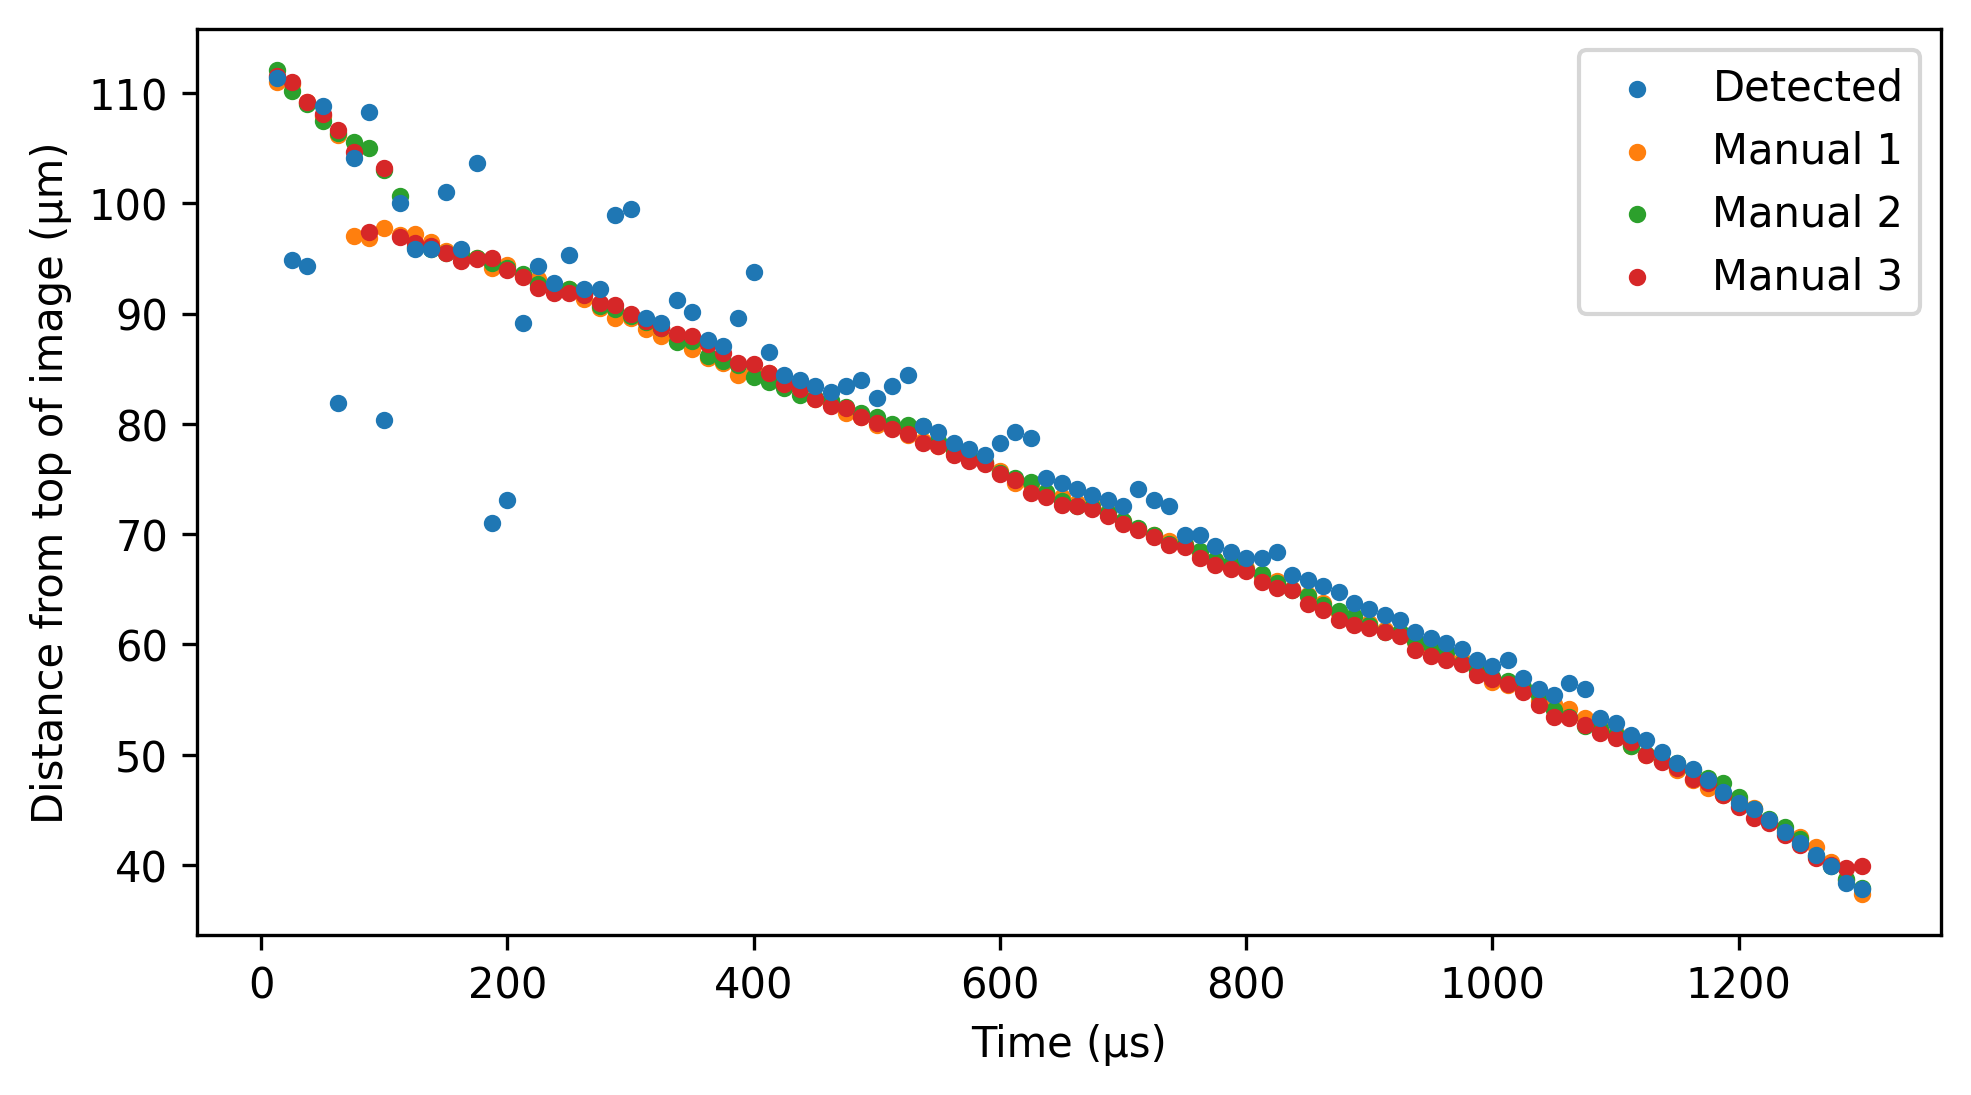
\includegraphics[width=0.75\textwidth]{figures/04/14-detected-vs-manual-3-12_shot01.png}
    \caption{
        \small\setstretch{1}
        Interfaces detected by the automated procedure (blue) compared with
        manually identified interfaces (orange, green, and red) for the
        208 W experiment. Interface location is defined by the distance from
        the bottom of the solid-liquid interface to top of the image,
        starting when the laser shuts off (t = 0 µs).
    }
    \label{fig/detected-aps-3}
\end{figure}

% -------------------------------------------------------------------------
\subsubsection{Rapid Solidification Results}
% -------------------------------------------------------------------------
The rapid solidification detection procedure and manual annotations are
performed on the data from three separate rapid solidification experiments.
For each of these
experiments, the mean and median velocity was calculated
for the major and minor axis lengths of the manually-measured and detected
ellipses.
In the first experiment, the average solidification velocities of the
three manually identified elliptical melt pools were calculated for the
major / minor axes as 2.164
m s\textsuperscript{-1} / 1.654 m s\textsuperscript{-1},
2.213 m s\textsuperscript{-1} / 1.690 m s\textsuperscript{-1}, and
2.172 m s\textsuperscript{-1} / 1.620 m s\textsuperscript{-1}. The
average major/minor axis velocities across all three measurements was
2.183 m s\textsuperscript{-1} / 1.655 m s\textsuperscript{-1} with medians of
2.167/1.580 m s\textsuperscript{-1}.

\begin{figure}[ht]
    \centering
    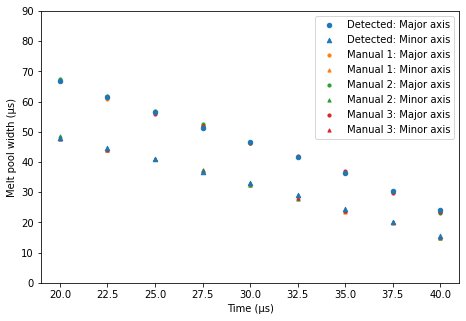
\includegraphics[width=0.75\textwidth]{figures/04/15-detected-vs-manual-03.png}
    \caption{
        \small\setstretch{1}
        Size of melt pools over time throughout the third rapid
        solidification experiment. The detected ellipses (blue) have a
        low deviation from the manually measured interfaces
        (orange, green, and red).
    }
    \label{fig/detected-dtem-1}
\end{figure}

In the second experiment, the average solidification velocities of the
three manually identified elliptical melt pools were calculated for the
major / minor axes as
2.268 m s\textsuperscript{-1} / 1.675 m s\textsuperscript{-1},
2.245 m s\textsuperscript{-1} / 1.773 m s\textsuperscript{-1}, and
2.234 m s\textsuperscript{-1} / 1.726 m s\textsuperscript{-1}. The
average major / minor axis velocities across all three measurements were
2.249 m s\textsuperscript{-1} / 1.725 m s\textsuperscript{-1} with medians
of 2.318/1.688 m s\textsuperscript{-1}.

\begin{figure}[ht]
    \centering
    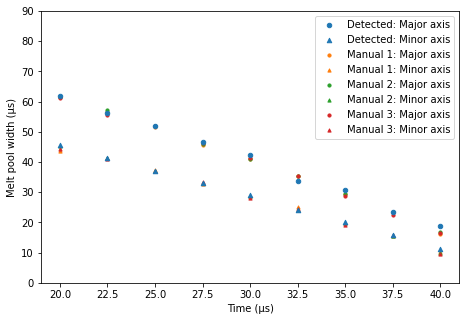
\includegraphics[width=0.75\textwidth]{figures/04/16-detected-vs-manual-04.png}
    \caption{
        \small\setstretch{1}
        Size of melt pools over time throughout the third rapid
        solidification experiment. The detected ellipses (blue) have a
        low deviation from the manually measured interfaces
        (orange, green, and red).
    }
    \label{fig/detected-dtem-2}
\end{figure}

In the third experiment, the average solidification velocities of the
three manually identified elliptical melt pools were calculated for the
major/minor axes as
2.665 m s\textsuperscript{-1} / 1.824 m s\textsuperscript{-1},
2.651 m s\textsuperscript{-1} / 1.871 m s\textsuperscript{-1}, and
2.602 m s\textsuperscript{-1} / 1.865 m s\textsuperscript{-1}. The
average major/minor axis velocities across all three measurements were
2.640 m s\textsuperscript{-1} / 1.853 m s\textsuperscript{-1} with medians
of 2.561 m s\textsuperscript{-1} / 1.856 m s\textsuperscript{-1}.

\begin{figure}[ht]
    \centering
    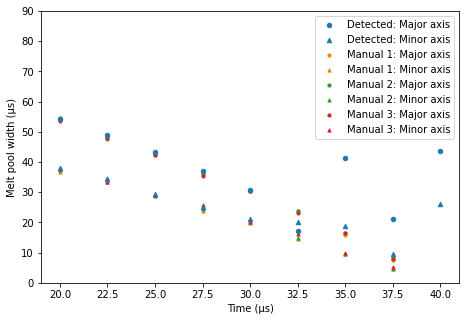
\includegraphics[width=0.75\textwidth]{figures/04/17-detected-vs-manual-09.png}
    \caption{
        \small\setstretch{1}
        Size of melt pools over time throughout the third rapid
        solidification experiment. The detected ellipses (blue) have a
        low deviation from the manually measured interfaces
        (orange, green, and red) until the end of the experiment.
    }
    \label{fig/detected-dtem-3}
\end{figure}


\subsection{Discussion}
This section discusses the detected and manually-measured
solidification velocity results for each
of the two type of experiments outlined in the previous section.

% -------------------------------------------------------------------------
\subsubsection{AM Simulator}
% -------------------------------------------------------------------------
Rather than relying on the mean and median velocities to
assess the AM simulator detection procedure, the deviations from the mean
manual velocity were analyzed for each individual manual measurement
and for the detected velocities. This was repeated for each of the three
experiments to quantify the variance of the velocity as a way to
quantitatively compare the automated procedure to the manual measurements.
% 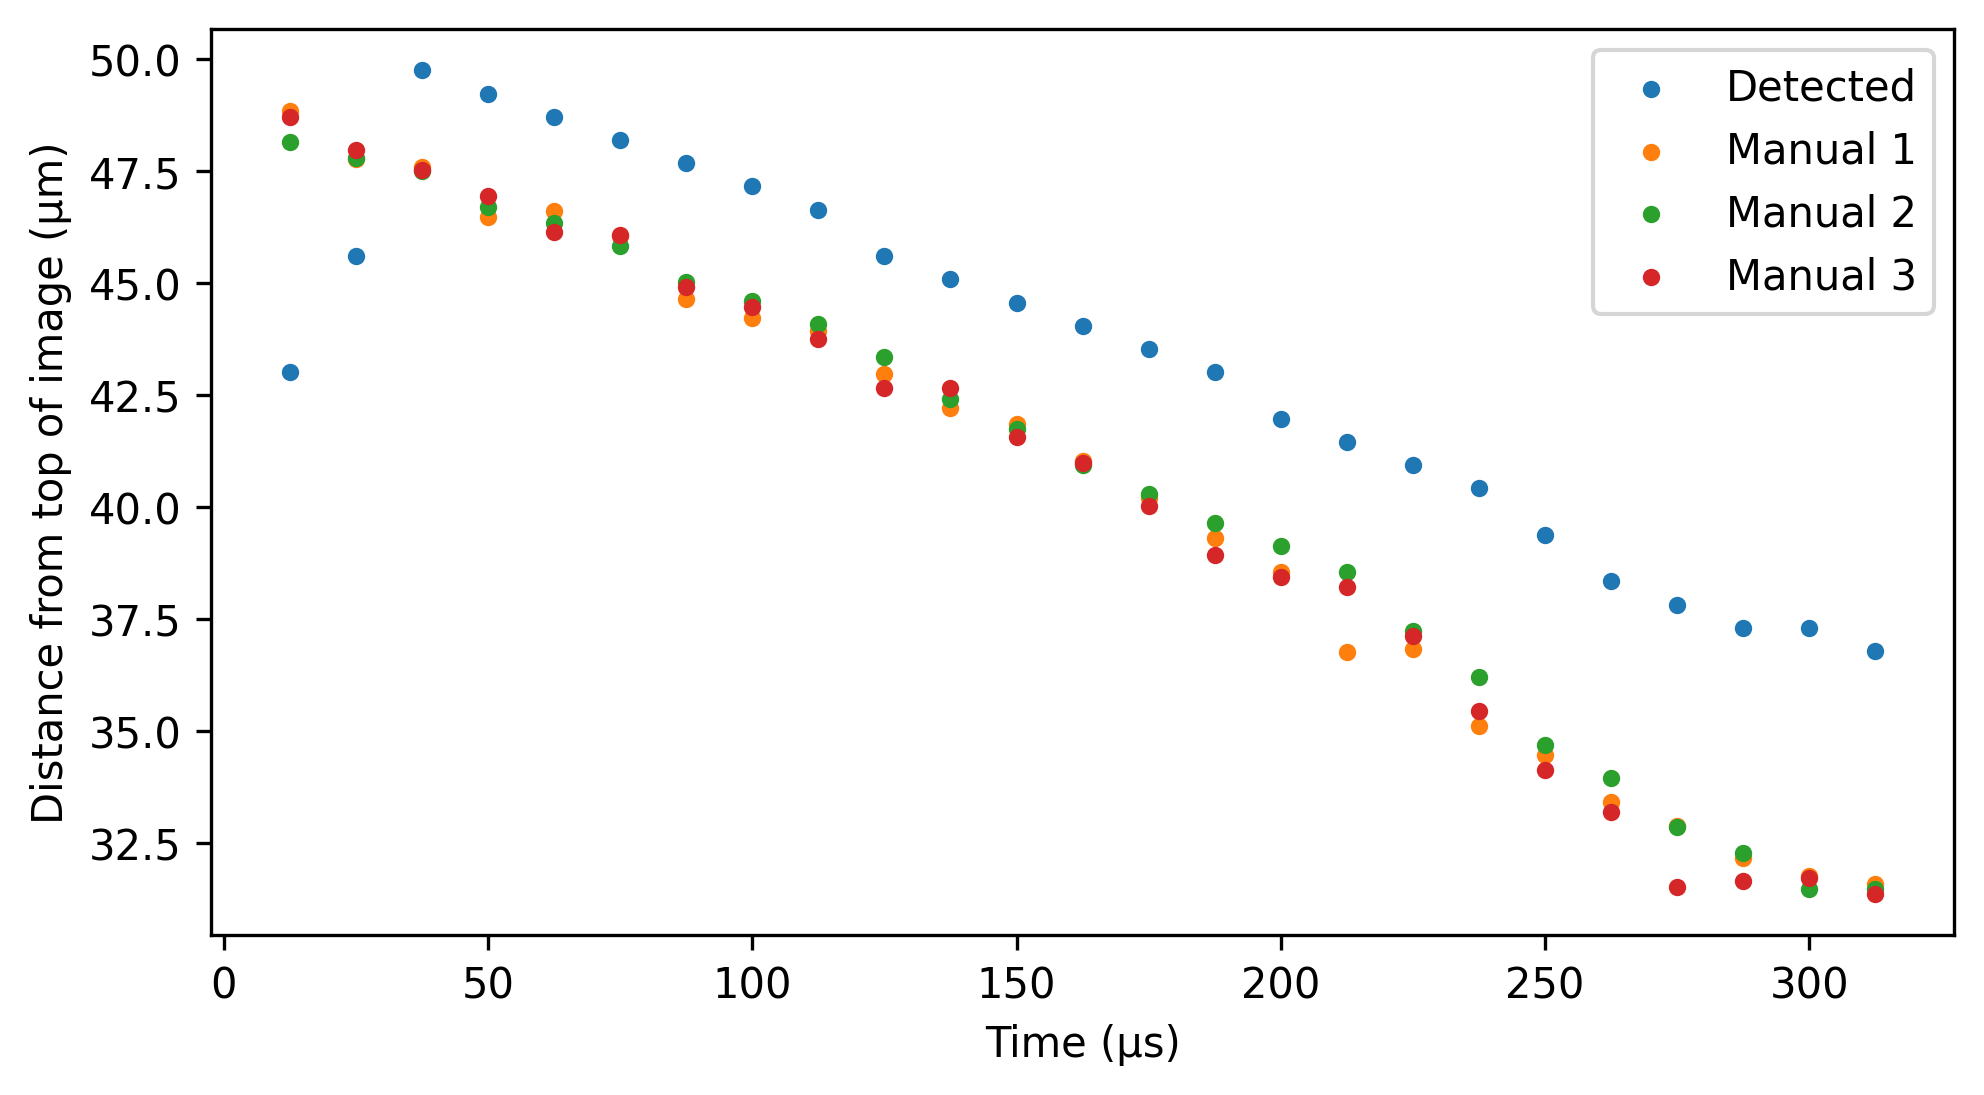
\includegraphics{figures/04/12-detected-vs-manual-1-10_shot05.png}
In the 104 W experiment, the mean velocities differ
drastically (0.021 m s\textsuperscript{-1} detected,
0.057 m s\textsuperscript{-1} manual), but less so
across the median values (0.041 m s\textsuperscript{-1} detected,
0.043 m s\textsuperscript{-1} manual),
suggesting there are outliers in the detected data that are skewing
the mean. This is further supported by the analyzing the average
deviations from the manual mean velocity (in terms of percent of the
manual mean: 78.800\% detected, 48.492\% manual). The average
deviations differ much like the mean velocities, however when considering
the spread of these deviations throughout the experiment, 58.333\% of
the manually measured velocities have a deviation lower than the average
manual deviation, whereas 87.5\% of the detected deviations are lower
than the same value. This indicates that the detected outliers are farther
from the manual mean than any of the individual manual measurements,
which is exemplified in \ref{fig/detected-aps-1} by the large
change in position (corresponding to a high velocity) across the first
three frames, compared to the more gradual change throughout the rest of the
experiment. This is especially interesting because the overall detected
interface position seems to be consistently about 2.5 µm higher than the
manually measured position. Since the interface still appears to be moving
at a rate similar to the manual measurements, this position discrepancy
could be the caused by the detection procedure capturing an optical artifact
slightly above the interface that nonetheless moved at the same rate.

% 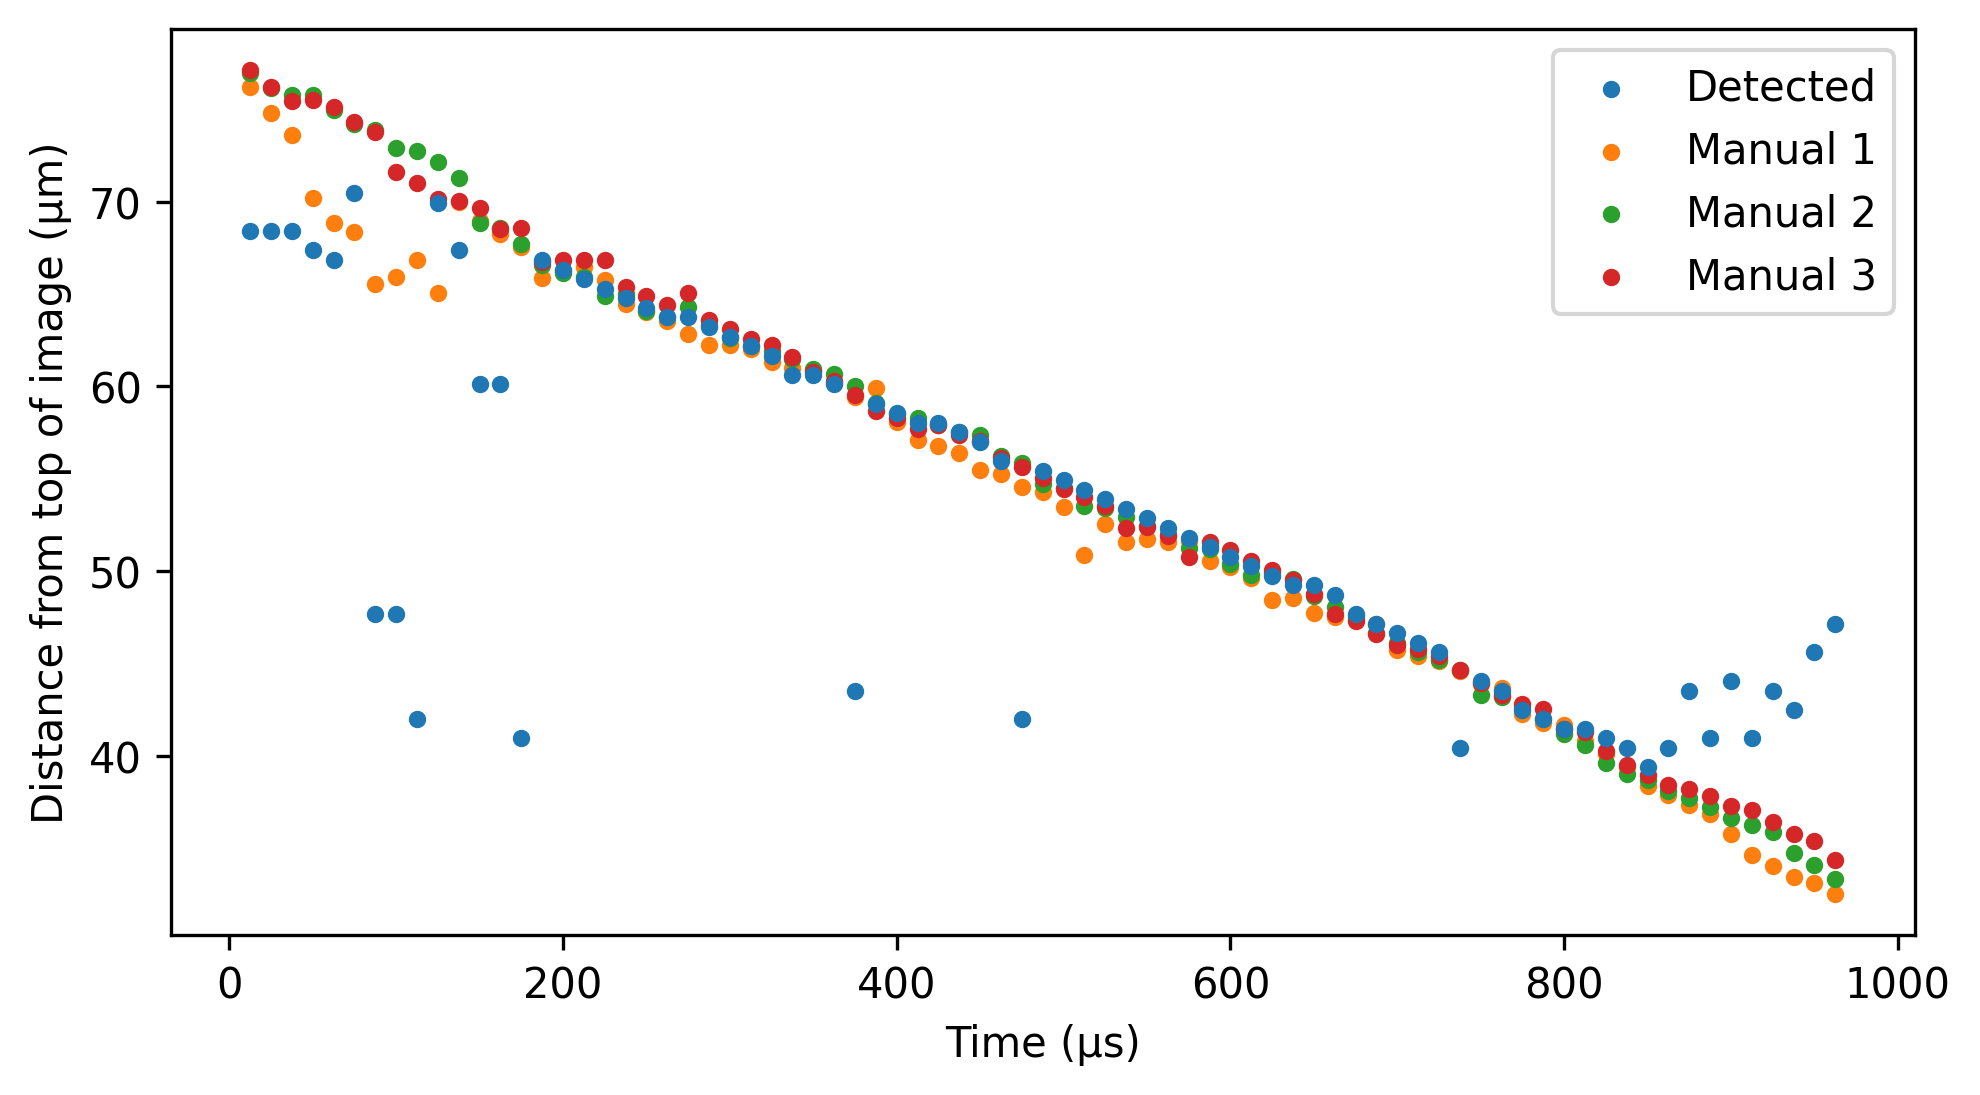
\includegraphics{figures/04/13-detected-vs-manual-2-06_shot01.png}
In the 156 W experiment, the average velocities differ
drastically (0.022 m s\textsuperscript{-1} detected,
0.046 m s\textsuperscript{-1} manual) but similar to
experiment 104 W less so across the median values
(0.041 m s\textsuperscript{-1} detected,
0.043 m s\textsuperscript{-1} manual).
The detected deviation from the manual mean
velocity is once again much larger than the manual deviation (in terms
of percent of the manual mean: 496.037\% detected, 69.798\% manual).
Considering the spread of these deviations yields slightly different
results in that 65.789\% of the manually measured velocities have a
deviation lower than the average manual deviation compared to the only
50.0\% of detected deviations. However, these 50.0\% of detected
deviations are also lower than half of the average manual deviation.
The outliers of the detected velocity may be further from the manual mean
than the manual measurements, but the fraction of the data that are
within the average manual deviation are much closer to the average than any
of the individual manual measurements. This can be seen in
\ref{fig/detected-aps-2} by the outliers of the detected positions
located farther away from the cluster of other data while the detected
positions closer to the rest of the data vary less across the frames than
the manual measurements. It is also worth noting that both the detected and
manual interface positions appear to be the most uncertain at the beginning
and end of the experiment, suggesting that the interface was harder to make
out than in the 104 W experiment, also supported by the fact that the
average manual deviation was higher for this experiment.

% 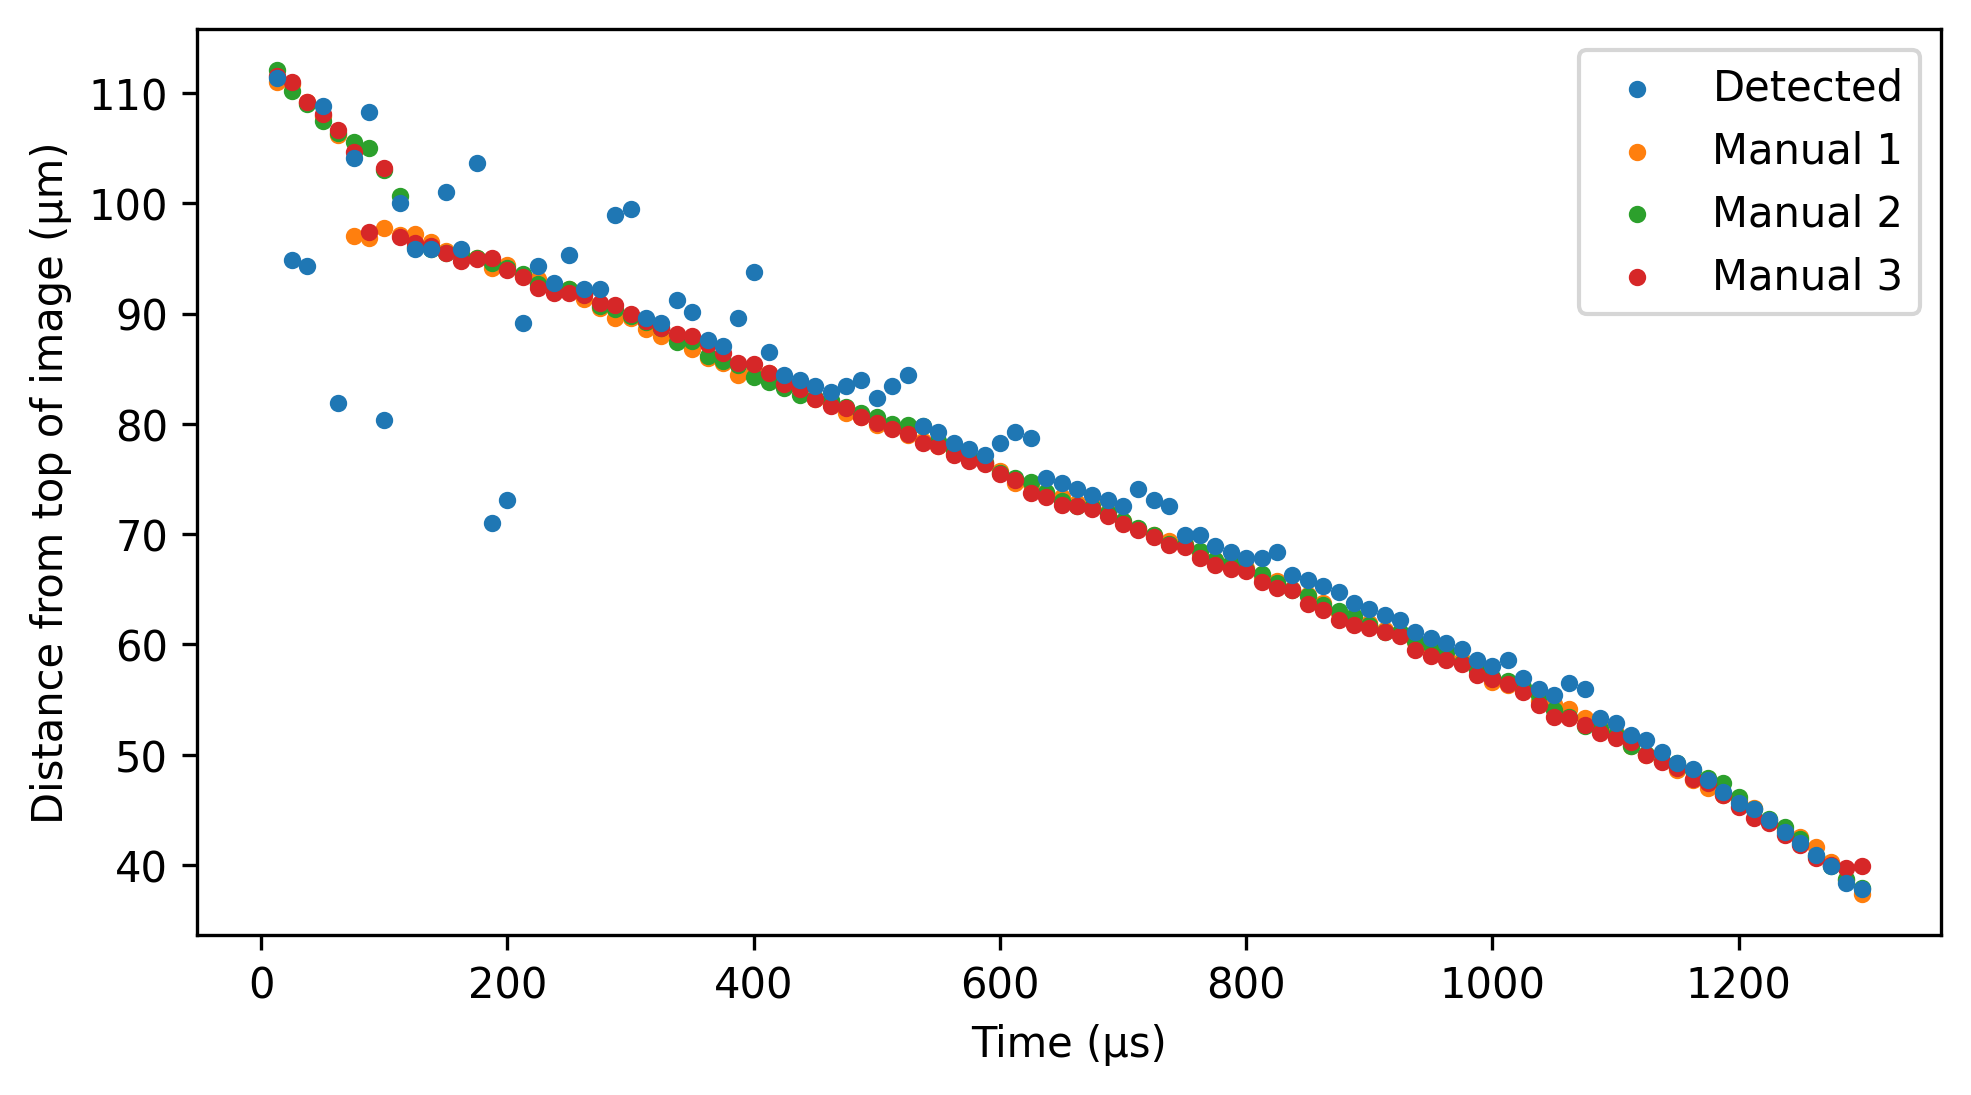
\includegraphics{figures/04/14-detected-vs-manual-3-12_shot01.png}
In the 208 W experiment, the mean velocities are
the same (0.057 m s\textsuperscript{-1} detected,
0.057 m s\textsuperscript{-1} manual). However, the median
values still differed (0.041 m s\textsuperscript{-1} detected,
0.052 m s\textsuperscript{-1} manual),
so the matching means is most likely an effect of the deviations
balanced on either side of the mean. Similar to the 156 W
experiment, the detected deviations from the manual mean velocity are much
higher than the manual measurements (in terms of percent of the
manual mean: 415.305\% detected, 56.777\% manual).
Much like the previous experiments, the outliers of the detected velocities
are much farther out from the rest of the data than the manually measured
velocities the experiment. 52.427\% of detected data has a deviation less
than the average manual deviation which is less than the 77.670\% of
the manually measured velocities, but still comparable. Comparing the data
that deviates within half the average manual deviation is even more similar
at 33.981\% of the detected velocities and 28.155\% of the manually
measured velocities. \ref{fig/detected-aps-3} shows the higher
deviation of the detected data far out from the mean like the previous
experiments, but a notable difference is that there appears to be a cusp in
the manually measured interface positions around 100 µs. This could be due
to a change in velocity of the S-L interface, but was more likely
due to a secondary interface that can appear in these experiments when a
melt pool becomes large enough to breach the edge of the sample. If the
sample breach happens at a different height than the minima of the melt pool,
the breach can appear to be a secondary interface. In this case, the breach
may have been more visible than the minima of the interface at the beginning
of the experiment. The first 100 - 200 µs of the experiment is also where
the detected position deviates from the mean the most.
As a side note, it is not entirely a coincidence that the median
velocity was the same for all
three experiments, as that value (0.041 m s\textsuperscript{-1})
corresponds to the 1 pixel/frame after converting pixels to µm with the
spatial resolution and frame number to µs with the experiment framerate.

% -------------------------------------------------------------------------
\subsubsection{Rapid Solidification}
% -------------------------------------------------------------------------
To assess the performance of the rapid solidification detection procedure,
the deviations from the mean manual
velocity were analyzed for the major and minor axes of the melt pools as
determined from each individual manual measurement
and for the detected procedure. This analysis was repeated for each of the
three DTEM experiments to characterize the performance of the procedure
compared to manual measurement.
% 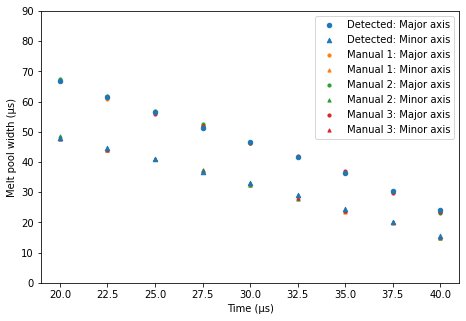
\includegraphics{figures/04/15-detected-vs-manual-03.png}
In the first experiment, the mean major / minor axis velocities
are similar (2.124 m s\textsuperscript{-1} / 1.619 m s\textsuperscript{-1}
detected, 2.183 m s\textsuperscript{-1} / 1.655 m s\textsuperscript{-1} manual),
and so are the median velocities
(2.167 m s\textsuperscript{-1} / 1.580 m s\textsuperscript{-1} detected,
2.101 m s\textsuperscript{-1} / 1.679 m s\textsuperscript{-1} manual).
The proximity of the mean to the medians for both the detected and manually
measured velocities suggests a small spread of the data, which is supported
by a lower deviation from the manual mean velocity (in terms of percent of the
manual mean for the major / minor axes: 7.9\% / 9.476\% detected,
13.543\% / 14.876\% manual). The data is distributed closely enough that it is
difficult to make out differences between the detected and manual data in
the plotted positions (\ref{fig/detected-dtem-1}).

% 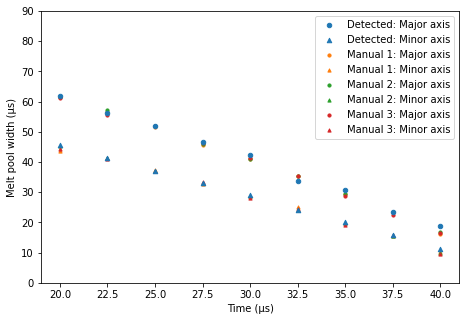
\includegraphics{figures/04/16-detected-vs-manual-04.png}
In the second rapid solidification experiment, the mean major / minor axis
velocities are also similar
(2.148 m s\textsuperscript{-1} / 1.719 m s\textsuperscript{-1} detected,
2.249 m s\textsuperscript{-1} / 1.725 m s\textsuperscript{-1} manual),
as are the median velocities
(2.028 m s\textsuperscript{-1} / 1.730 m s\textsuperscript{-1} detected,
2.318 m s\textsuperscript{-1} / 1.688 m s\textsuperscript{-1} manual).
The deviation from the manual mean velocity is also low (in terms of percent
of the manual mean for the major / minor axes:
24.001\% / 6.248\% detected, 10.331\% / 15.954\% manual),
however the deviation of the manual measurements is slightly larger,
as can be seen by some outliers in the the position data
(\ref{fig/detected-dtem-2}).

% 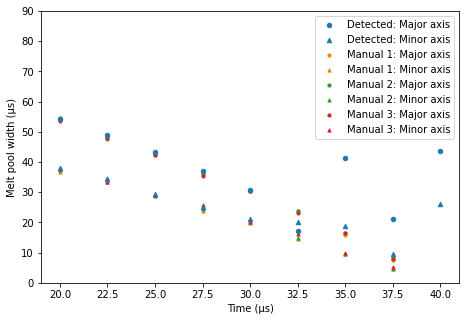
\includegraphics{figures/04/17-detected-vs-manual-09.png}
In the third rapid solidification experiment, the mean major / minor axis
velocities are (1.893 m s\textsuperscript{-1} / 1.628 m s\textsuperscript{-1}
detected, 2.640 m s\textsuperscript{-1} / 1.853 m s\textsuperscript{-1} manual),
and the median velocities
(2.494 m s\textsuperscript{-1} / 1.683 m s\textsuperscript{-1} detected,
2.561 m s\textsuperscript{-1} / 1.856 m s\textsuperscript{-1} manual).
The detected procedure had a larger deviation from the manual measurements
than in either of the two previous experiments. The deviations from the
manual mean velocity are much higher (in terms of percent of the manual
mean for the major / minor axes:
119.014\% / 42.621\% detected, 13.365\% / 14.290\% manual).
It is worth noting that in this experiment,
the manual measurements only recorded eight frames
in which the elliptical melt pool was manually measured because the sample
completely solidified before the last frame. As can be seen in the position
data, the detected melt pool size deviates more from the manual measurements
at the end of the experiment (\ref{fig/detected-dtem-3}).
This suggests the detection procedure is less effective when the melt pool is
near closing, most likely because the shape of the melt pool is lost within
the noise of the image.


\subsection{Conclusions}
Methods for calculating solidification velocities are important
for accurately predicting microstructures in AM-like processes
and linking those microstructures to processing parameters.
Characterization tools like synchrotron
x-radiography and DTEM enable high spatial and temporal resolution in-situ
monitoring of solidification, but the large amounts of data these
techniques yield require difficult manual analysis to retrieve
quantitative information like solidification velocities. Tracking and
annotating image data manually introduces human bias and error that can be
inconsistent across measurements and users. Reasons for these
inconsistencies include subjective judgement calls, personal preferences,
miscommunications, and user fatigue. These sources of error in
measurements can be difficult, and in some cases nearly impossible, to
quantify. The automated detection techniques presented in this work
explored the possibility of a consistent method of analyzing image data
from solidification experiments, while also reducing the effect of bias on
the collected data. Two procedures were presented in this work for
automating the detection of S-L interfaces and calculating solidification
velocities, and each procedure was applied to three separate experiments.
The first procedure determined S-L interface positions in synchrotron
x-radiography images from simulated AM experiments. The second procedure
automated the detection of S-L interfaces for frames in three
separate DTEM images depicting thin film rapid solidification.
Each procedure was similar but each took a slightly different approach to
interface detection.

The simulated AM procedure performed adequately as compared to manual
measurements.
The detection procedure returned drastically different mean velocities from
the manual measurements for the 104 W and 156 W experiments, however the median
detected and manual velocities are similar, suggesting that the differing
means are because of outliers in the velocity, which is supported by the
significantly higher detected deviation from the manual mean velocity
compared with the manual deviation from the manual mean velocity.
In the 208 W experiment, the detected mean velocity is the same as the
manual velocity, but the median velocities differed. Similar to the 104 W
and 156 W experiments, the detected deviation from the manual mean is much
higher than the manual deviation. This suggests that the 208 W experiment
has a similar problem with the outliers, but that the outlying detected
velocities are more evenly distributed both above and below the manual
mean velocity.

The rapid solidification procedure performed well as compared to the manual
measurements. For the first and second experiments, the mean and median values
are both similar with low deviations from the manual mean velocity. In the
third experiment, the detected mean velocity differs more than either of the
previous two experiments, but the median values are still similar. The
detected deviation from the manual mean is also higher in this experiment.
Upon closer analysis, the detected velocity has the highest deviation from
the manual mean velocity towards the end of the experiment. This is
significant because the third experiment fully solidified
before the other two experiments. The melt pool does not even show up
in the final frame. This suggests the procedure does best when
the melt pool is larger and more distinguishable from noise.

The simulated AM procedure did not include any kind of a fit optimization step.
The rapid solidification procedure, which did optimize the fit of the detected
melt pool, was more successful in matching the manually measured velocities.
If a similar optimization step could be included in the simulated AM procedure,
there may be an increase in detection accuracy.
In addition, the fitting of the interfaces to parameterized shapes would allow
the solidification velocity to be calculated at multiple points along the
interfaces. This is not currently possible since the procedure
measures the location of the interface based on the bottom of the interface,
thus only allowing for the vertical solidification velocity
to be calculated.

While this work doesn't claim that these data extraction and analysis methods
remove human biases altogether (the procedures were written by a human, after
all), a procedure deterministically run by a computer
makes the method of extracting data more consistent. The nature of the
procedure development may also prompt researchers to more
carefully consider biases introduced through their methods.
Each step in the procedure must be actively considered to be incorporated,
whereas unconscious passivity is possible in manual actions
performed in a repetitive manner.
The less laborious effect of automated procedures may also benefit researchers
by allowing them to more quickly and easily test the effects
of small changes to data extraction and analysis, as opposed to the significant
time and effort to reproduce changes to manual routines. This reduced barrier
to iteration could encourage researchers to test a larger number of iterations
data extraction methods, potentially even resulting in more refined results.

\subsection*{Acknowledgements}
A special thanks to the beamline scientists at the Advanced Photon Source
that make themselves available at odd hours to keep experiments at the
facility running smoothly and to the students of the Center for Advanced
Non-Ferrous Structural Alloys that agreed to work all the other odd hours to
run the experiments and collect the simulated AM data.



% -------------------------------------------------------------------------
%   Chapter 5
% -------------------------------------------------------------------------
\newpage
\chapter{
    IMPLEMENTING EDGE STRENGTH CORRECTIONS TO IMPROVE SEGMENTATION OF
    IRREGULARLY-SHAPED, MULTI-SIZED, AND TIGHTLY-CLUSTERED PARTICLES
    \label{ch/seg}
}
% \section{Abstract}
Watershed segmentation algorithms are useful tools
to separate features in an image from one another, enabling
more targeted analyses. However, these algorithms
often do not achieve expected results for multi-sized or
irregularly-shaped particles, or particles clustered tightly together without
strongly defined edges along contact surfaces.
This chapter presents an image processing procedure
implemented in Python (with
libraries including \textit{scikit-image}, \textit{imageio}, \textit{NumPy},
and \textit{SciPy}) to improve the results of a
watershed segmentation algorithm. The proposed procedure involves application
of a preprocessing routine and custom algorithm which utilizes Delaunay
triangulation to merge segmented regions based on
edge strength between the regions.
The resulting merged-region segmentation results are calculated to more
closely match a manual segmentation than a typical watershed segmentation
on its own. The procedure is tested on a 2D radiograph sliced from a 3D
x-ray computed tomography (XCT) dataset depicting irregularly-shaped and
multi-sized sand grains that are tightly clustered with a polymer binder.


% Implementing edge strength corrections to improve segmentation of
% irregularly-shaped, multi-sized, and clustered particles in
% two-dimensional images
\subsection{Introduction}
Image segmentation often plays a crucial role in digital image processing
workflows. Segmentation enables the extraction of quantitative information
from images that is only qualitatively available through visually analysis
alone. Segmentation can be split into two categories: semantic segmentation
and instance segmentation. In semantic segmentation, an image is separated,
or segmented, into classes for analysis, often the regions of interest
(the foreground) and the background.
The result of this type of segmentation is a binary
image, so this process can be referred to as binarization. A simple way to
binarize an image is by selecting a threshold value such that pixels with an
intensity above this value are categorized as one of the binary labels,
while the pixels with an intensity below the thresholding value are
categorized as the second label. The threshold value is often selected
manually, but an algorithm can also be used to calculate this value. A
useful and well-known thresholding algorithm is Otsu's method \cite{Otsu1979},
which computes an
optimal threshold value by analyzing the image histogram. The histogram is
split into classes at different values, and a ``goodness'' factor, defined
by considering within-class and between-class variances, is optimized to
determine the threshold value.

The second type of segmentation, instance segmentation, is used to separate
specific instances of a class within an image.
Instance segmentation can
separate features within the foreground from one another to enable analyses
including feature locations, sizes, and shapes.
In some cases, it may be possible to separate multiple objects based
on gray value alone by setting multiple threshold values,
however instance segmentation can also be performed by analyzing the
morphology of a semantic segmentation.
One such method involves
morphological watersheds, and is typically referred to as watershed segmentation
\cite{Beucher1979,Serra1988,Soille1990sigproc,Soille1990viscomm,Beucher1992}.
Watershed
segmentation algorithms take their name from the analogy of ``flooding'' an
image by interpreting each intensity value as a height, as if the image is
describing a topographic surface. When a flooding operation is performed
algorithmically, the local minima of the image act as ``catchment basins''
which fill until a flood reaches a neighboring flood, at which point a
``dam'' is created to prevent the floods from merging. After this process is
completed, the lines representing the dams remain, thus segmenting the
image. As most images wouldn't appear to represent a logical
three-dimensional surface, a transformation of some kind is often applied
before watershed segmentation. This can be done using the Euclidean
distance transformation, which maps each foreground pixel of a binary
image to an intensity representing the distance to the nearest background
pixel \cite{Danielsson1980}. Distance transformations are usually inverted
before applying a
watershed segmentation algorithm so the pixels farthest away from the
background (local maxima) will be converted to local minima
that will be filled first by the flooding simulation.

Watershed segmentation algorithms can operate by providing a list of
markers which seed the catchment basins used in the algorithm
\cite{Moga1998,Parvati2008}. These
markers provide locations to begin algorithmic flooding at the same time,
regardless of the pixel intensities (``heights'') of these locations.
Markers can thus be
thought of as ``pour points.'' This can be useful to control
over-segmentation (more segmented regions than expected) and
under-segmentation (fewer segmented regions than expected) because in
marker-defined watershed segmentation, the number of markers determines
the number of catchment basins and therefore the number of final segmented
regions. The limitations of segmenting an image via watershed algorithm
are often related to the method employed to define the markers. A
common method of generating markers is to calculate the minima of the
inverse distance transformation. However, this can lead to spurious local
minima for irregularly shaped and/or clustered particles, resulting in
over-segmentation \cite{Sun2017}. In these cases, rather than calculate
all local minima, \textit{h}-minima can be calculated such that each minima
is a value \textit{h} above any surrounding minima \cite{Cheng2009,Jung2010}.

A downside to using \textit{h}-minima for marker generation is that this can
suppress legitimate minima corresponding to smaller particles when a variety
of particle sizes are present. This has been addressed with an adaptive
\textit{h}-minima method for selecting watershed markers \cite{Burgmann2022}.
This method uses dynamic \textit{h} values determined by setting a lower and
upper \textit{h} value for the intensity range of the image. For an inverse
distance transform, the \textit{h}
value range is set such that minima with lower intensities (i.e., points
farther from edges) have a higher \textit{h} value than minima with higher
intensities (i.e., points closer to edges). This translates to allowing
minima to be selected that are closer together around small objects in the
image but farther apart around larger objects. Another method is to remove
minima within a set radius determined by the comparison of intensities
between each minima and the surrounding minima \cite{Sun2017}.
This is based on the
assumption that spurious minima are caused by irregularly-shaped or
overlapping objects. Rather than suppress markers before seeding a
watershed algorithm, another method addresses over-segmentation by
detecting strong edges using the Canny edge filter and merging segmented
regions if the shared boundary does not exist on an edge, as long as the
edge is strongly defined \cite{Canny1986,Kim2003}.


\subsection{Methods}
% -------------------------------------------------------------------------
A typical watershed segmentation is performed to determine if a difficult
segmentation can take advantage of one of the previously mentioned
marker generating methods, based on whether segmenting based on distance
transform maxima results in over- or under-segmentation.
In a typical watershed
segmentation routine, an image is semantically segmented and represented
as a binary image, the binary
image undergoes a distance transformation, and the maxima of the distance
transformation is used to generate markers to seed the watershed
segmentation. This type of routine is tested with an image of sand grains
to see if the resulting segmentation meets expectations for an image of
irregularly-shaped, multi-sized, and tightly-clustered sand grains
(\ref{fig/05/raw-bw}.a). This image is loaded from file using the
Python package \textit{imageio} and converted to a \textit{NumPy}
array \cite{imageio,numpy}. As an array, the image is
binarized using the Otsu thresholding algorithm
implemented in \textit{scikit-image} (\ref{fig/05/raw-bw}.b)
\cite{Otsu1979,skimage}.

\begin{figure}[ht]
    \centering
    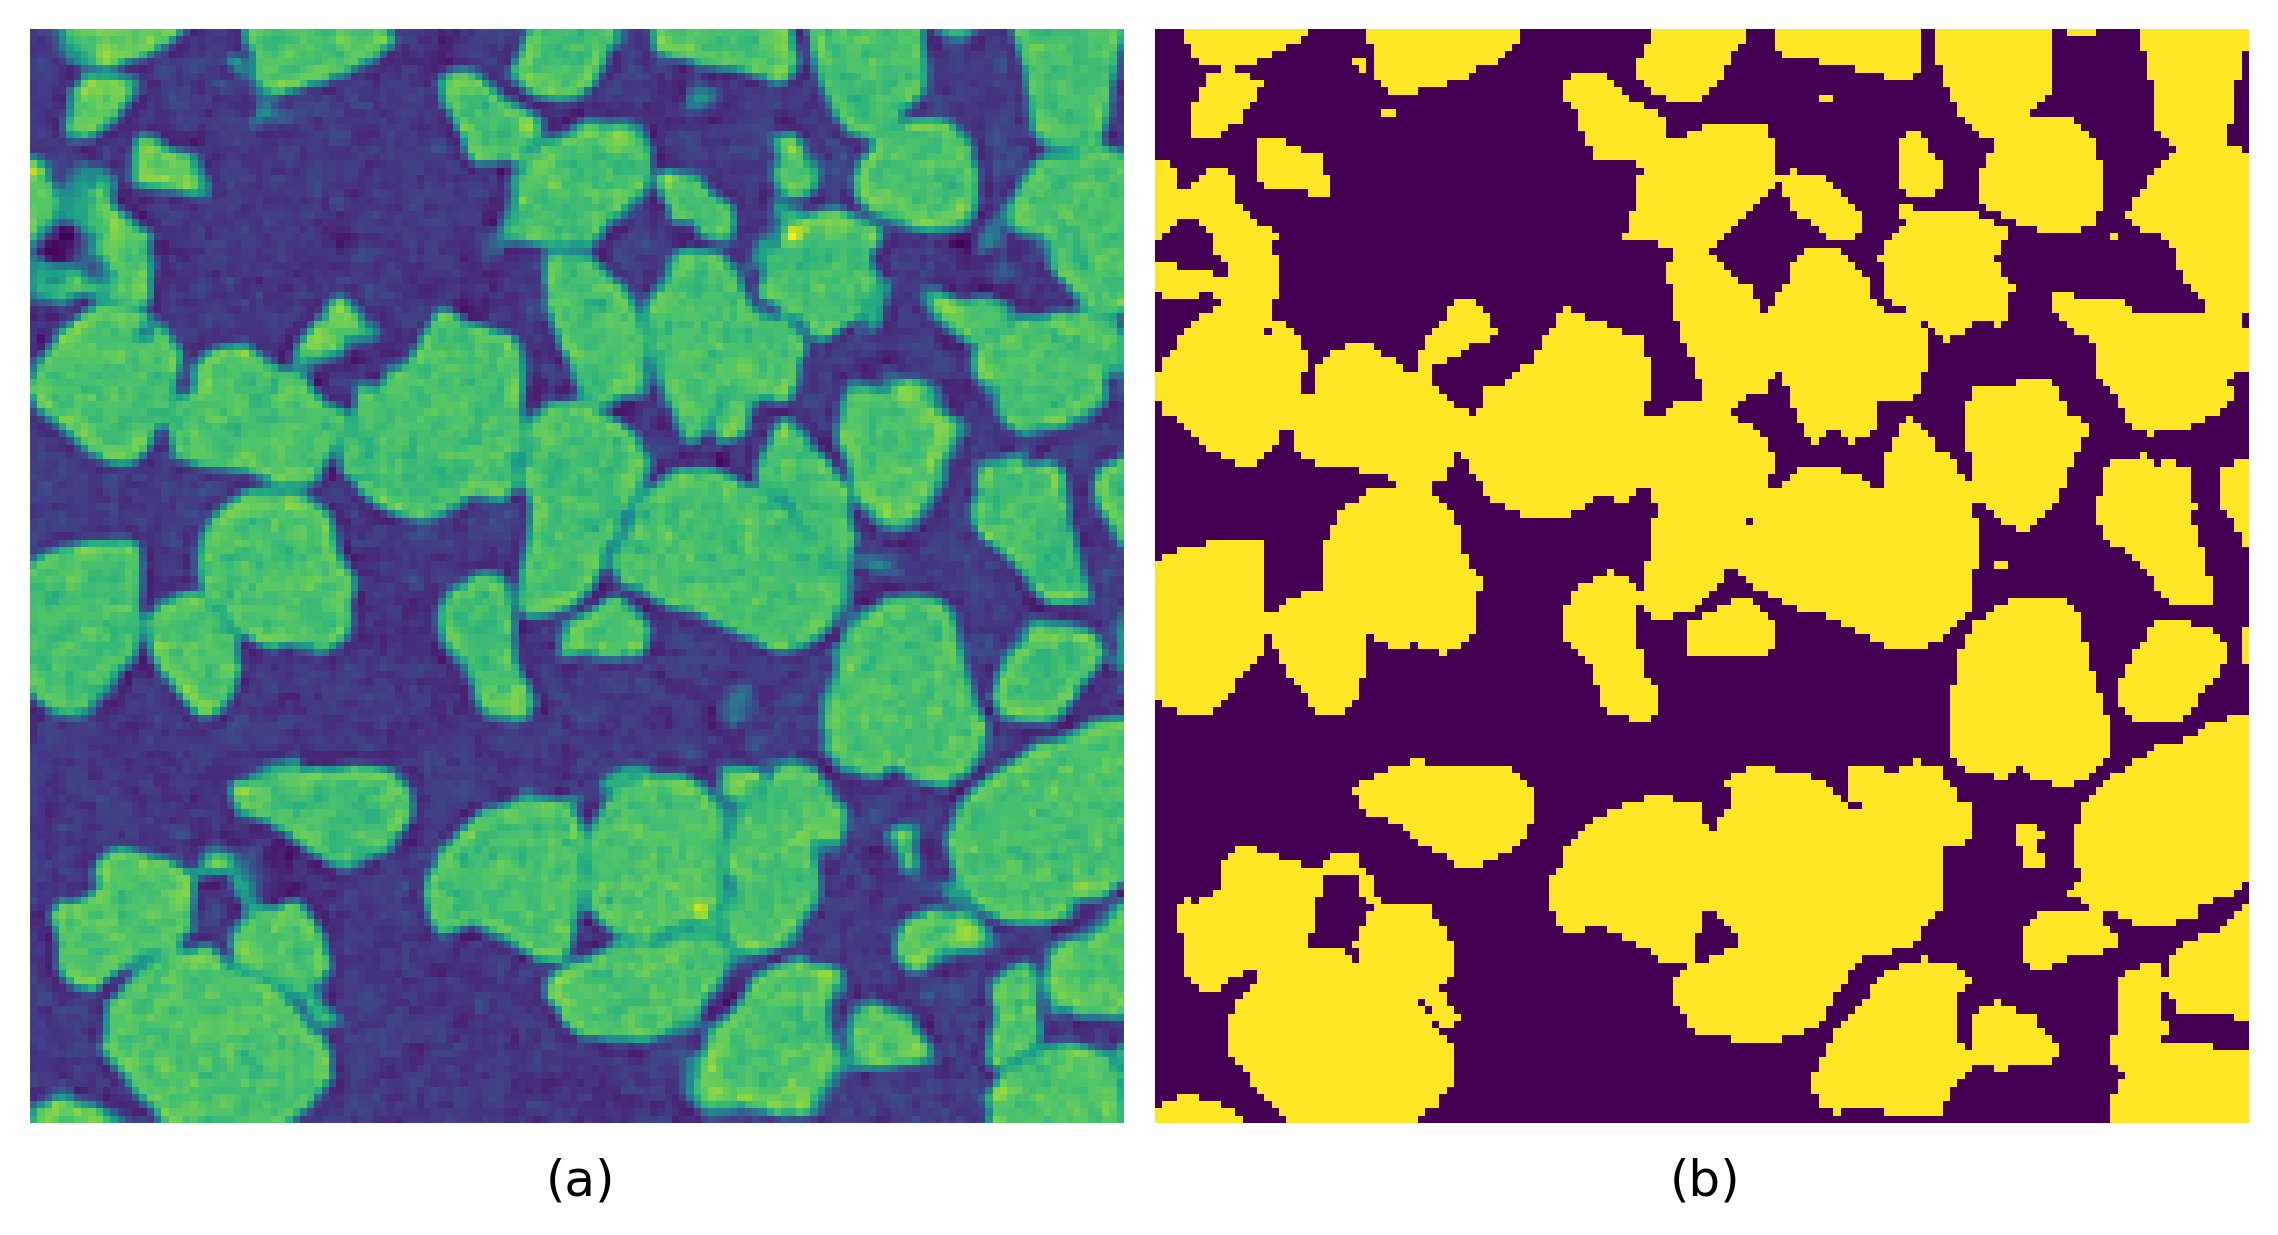
\includegraphics[width=0.75\textwidth]{figures/05/01-raw-bw.png}
    \caption{
        \small\setstretch{1}
        (a) Raw image depicting sand particles sliced from a 3D CT scan.
        (b) Binary image created from the raw image with Otsu thresholding.
        Yellow regions represent foreground pixels (valued one) while purple
        regions represent background pixels (valued zero).
    }
    \label{fig/05/raw-bw}
\end{figure}

After creating the binary image, a series of markers are generated which
will be used to seed the watershed segmentation. The distance of each
foreground pixel to the nearest background pixel calculated using the
Euclidean distance transformation implemented in \textit{SciPy} \cite{scipy}.
This distance
transformation is inverted to pass to the watershed algorithm. The local
maxima of this distance transform (equivalent to the local minima of the
inverted distance transformation) correspond to the points farthest from
the edges of the binary image (\ref{fig/05/typical}.b).
In the case of some of the
oblong particles present in the image, detecting all the local minima
resulted in connected groups of redundant minima where multiple
neighboring pixels exist at the same distance from the edge of the binary
image. This was addressed by using the \textit{scikit-image} functions
\textit{label} and \textit{regionprops} to retain only the centermost
point of connected minima. Once disconnected and non-redundant minima
were obtained, these points were used as markers to seed a watershed
algorithm implemented in \textit{scikit-image}.
The resulting segmented regions (\ref{fig/05/typical}.c) do not meet
expectations based on the visually discernible particles in the original
image. Since the segmented regions are over-segmented in some places and
under-segmented in others, the methods from literature outlined previously
cannot correct the segmentation.

\begin{figure}[ht]
    \centering
    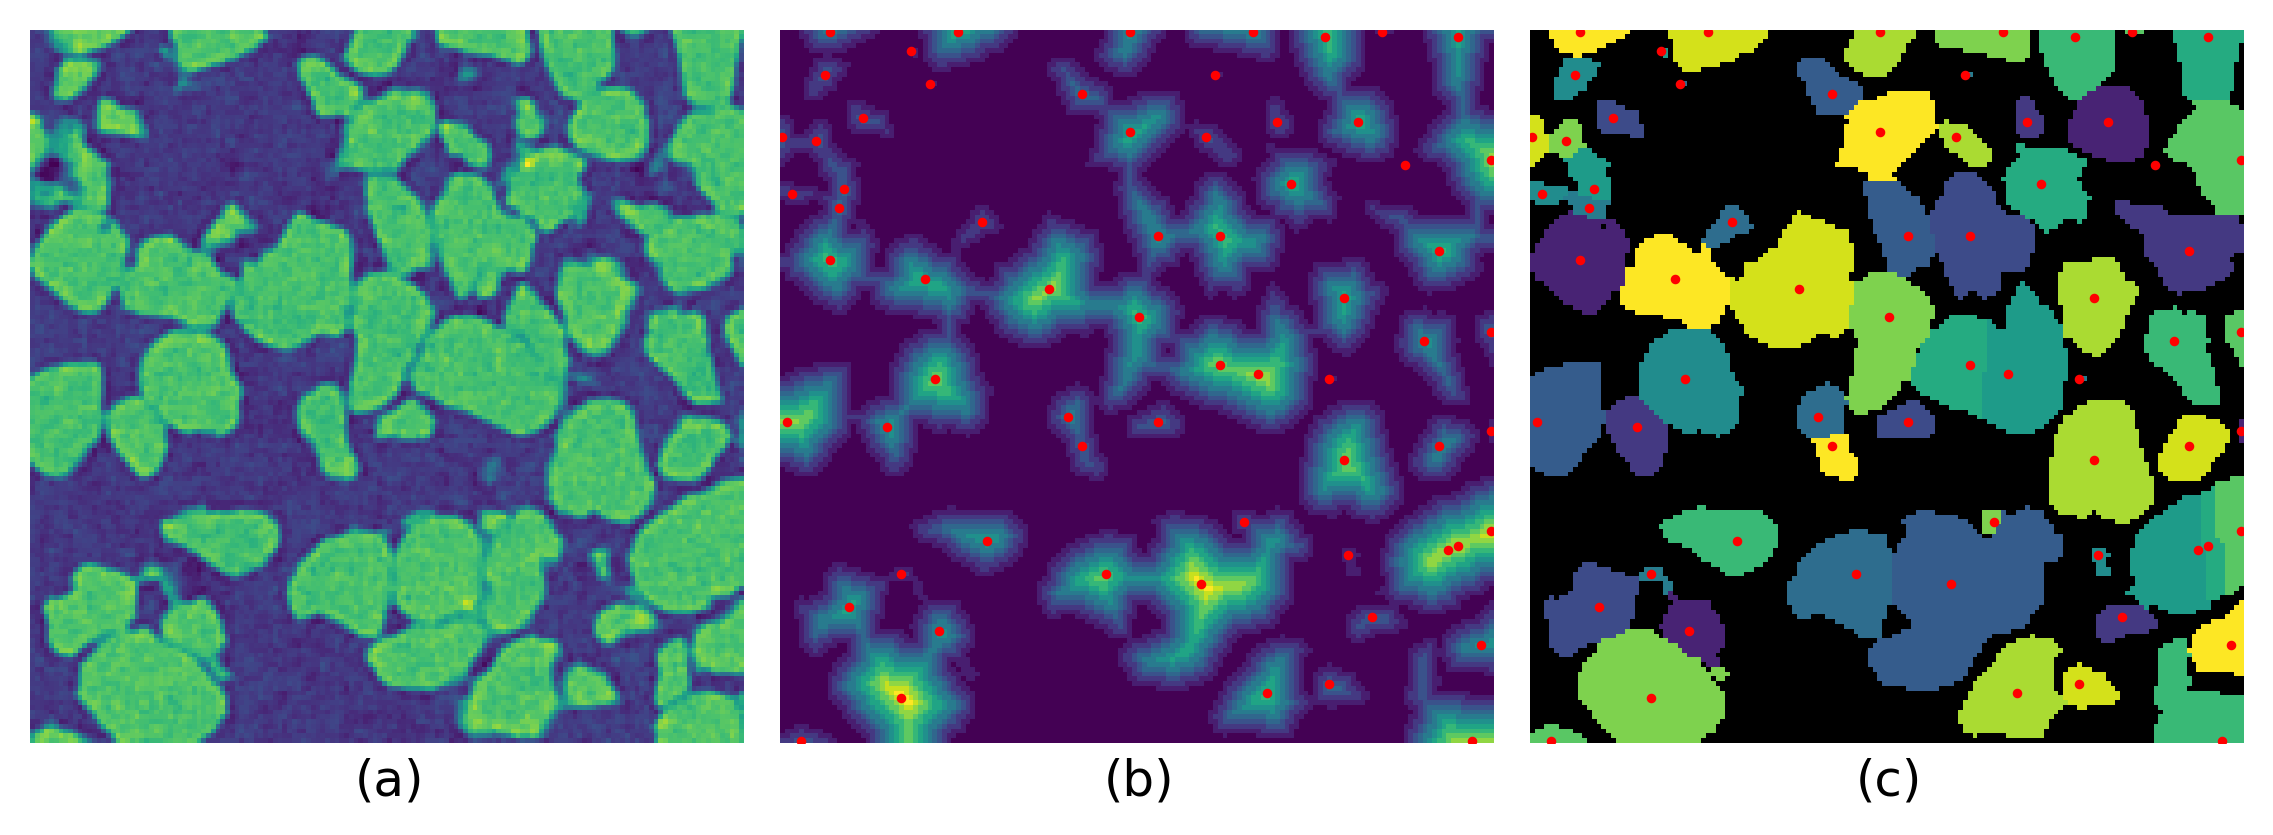
\includegraphics[width=0.75\textwidth]{figures/05/02-typical-routine.png}
    \caption{
        \small\setstretch{1}
        (a) Image depicting sand particles sliced from a 3D CT scan.
        (b) Euclidean distance transformation of Otsu-binarized image
        (\ref{fig/05/raw-bw}.b) with local maxima denoted by red points.
        (c) Watershed segmentation of inverted Euclidean distance
        transformation seeded by local minima of the inverted distance
        transformation (red points).
    }
    \label{fig/05/typical}
\end{figure}

% -------------------------------------------------------------------------
\subsubsection{Adding a Preprocessing Routine to Generate New Markers}
% -------------------------------------------------------------------------
To achieve segmentation results that align more closely with expectations,
the strategy of the procedure outlined in this work is to first create a set
of markers to intentionally over-segment the image, followed by a
subsequent step of determining region neighbors and correcting the
over-segmentation by merging neighboring regions
according to edge strength. This will ensure there is not a combination of
over- and under-segmentation occurring. New markers are needed
to achieve this over-segmentation such that each particle in the original
image contains at least one marker to prevent under-segmentation.
A preprocessing routine is employed to
generate these markers. The original image is rescaled between the 5th and
95th percentiles (\ref{fig/05/routine}.b).
Histogram equalization from \textit{scikit-image} is
performed on the rescaled image to enhance the intensities of the maxima
within the particles (\ref{fig/05/routine}.c).
Histogram equalization spreads out the values of the image
across the entire range, allowing for the creation of a binary image that
contains only the innermost regions of the particles. To create this
binary image, the multiple-class functionality of Otsu's method
implemented in \textit{scikit-image} is used to separate the image into three
classes. This can be visualized as a ternary image
(\ref{fig/05/routine}.d), however
only the regions above the uppermost threshold value are selected to
create the binary image. Holes within the created regions are filled using
the function \textit{binary\textunderscore fill\textunderscore holes}
from the multidimensional image processing
submodule in \textit{SciPy} (\ref{fig/05/routine}.e).
This maximizes the distances calculated via
distance transformation operating on the multi-Otsu binary image
(\ref{fig/05/routine}.f). The local maxima of this distance
transformation are useful for this
routine because they over-represent the particles in the image
(i.e., more markers than particles), which will result in the
over-segmentation desired at this stage of the procedure.

\begin{figure}[ht]
    \centering
    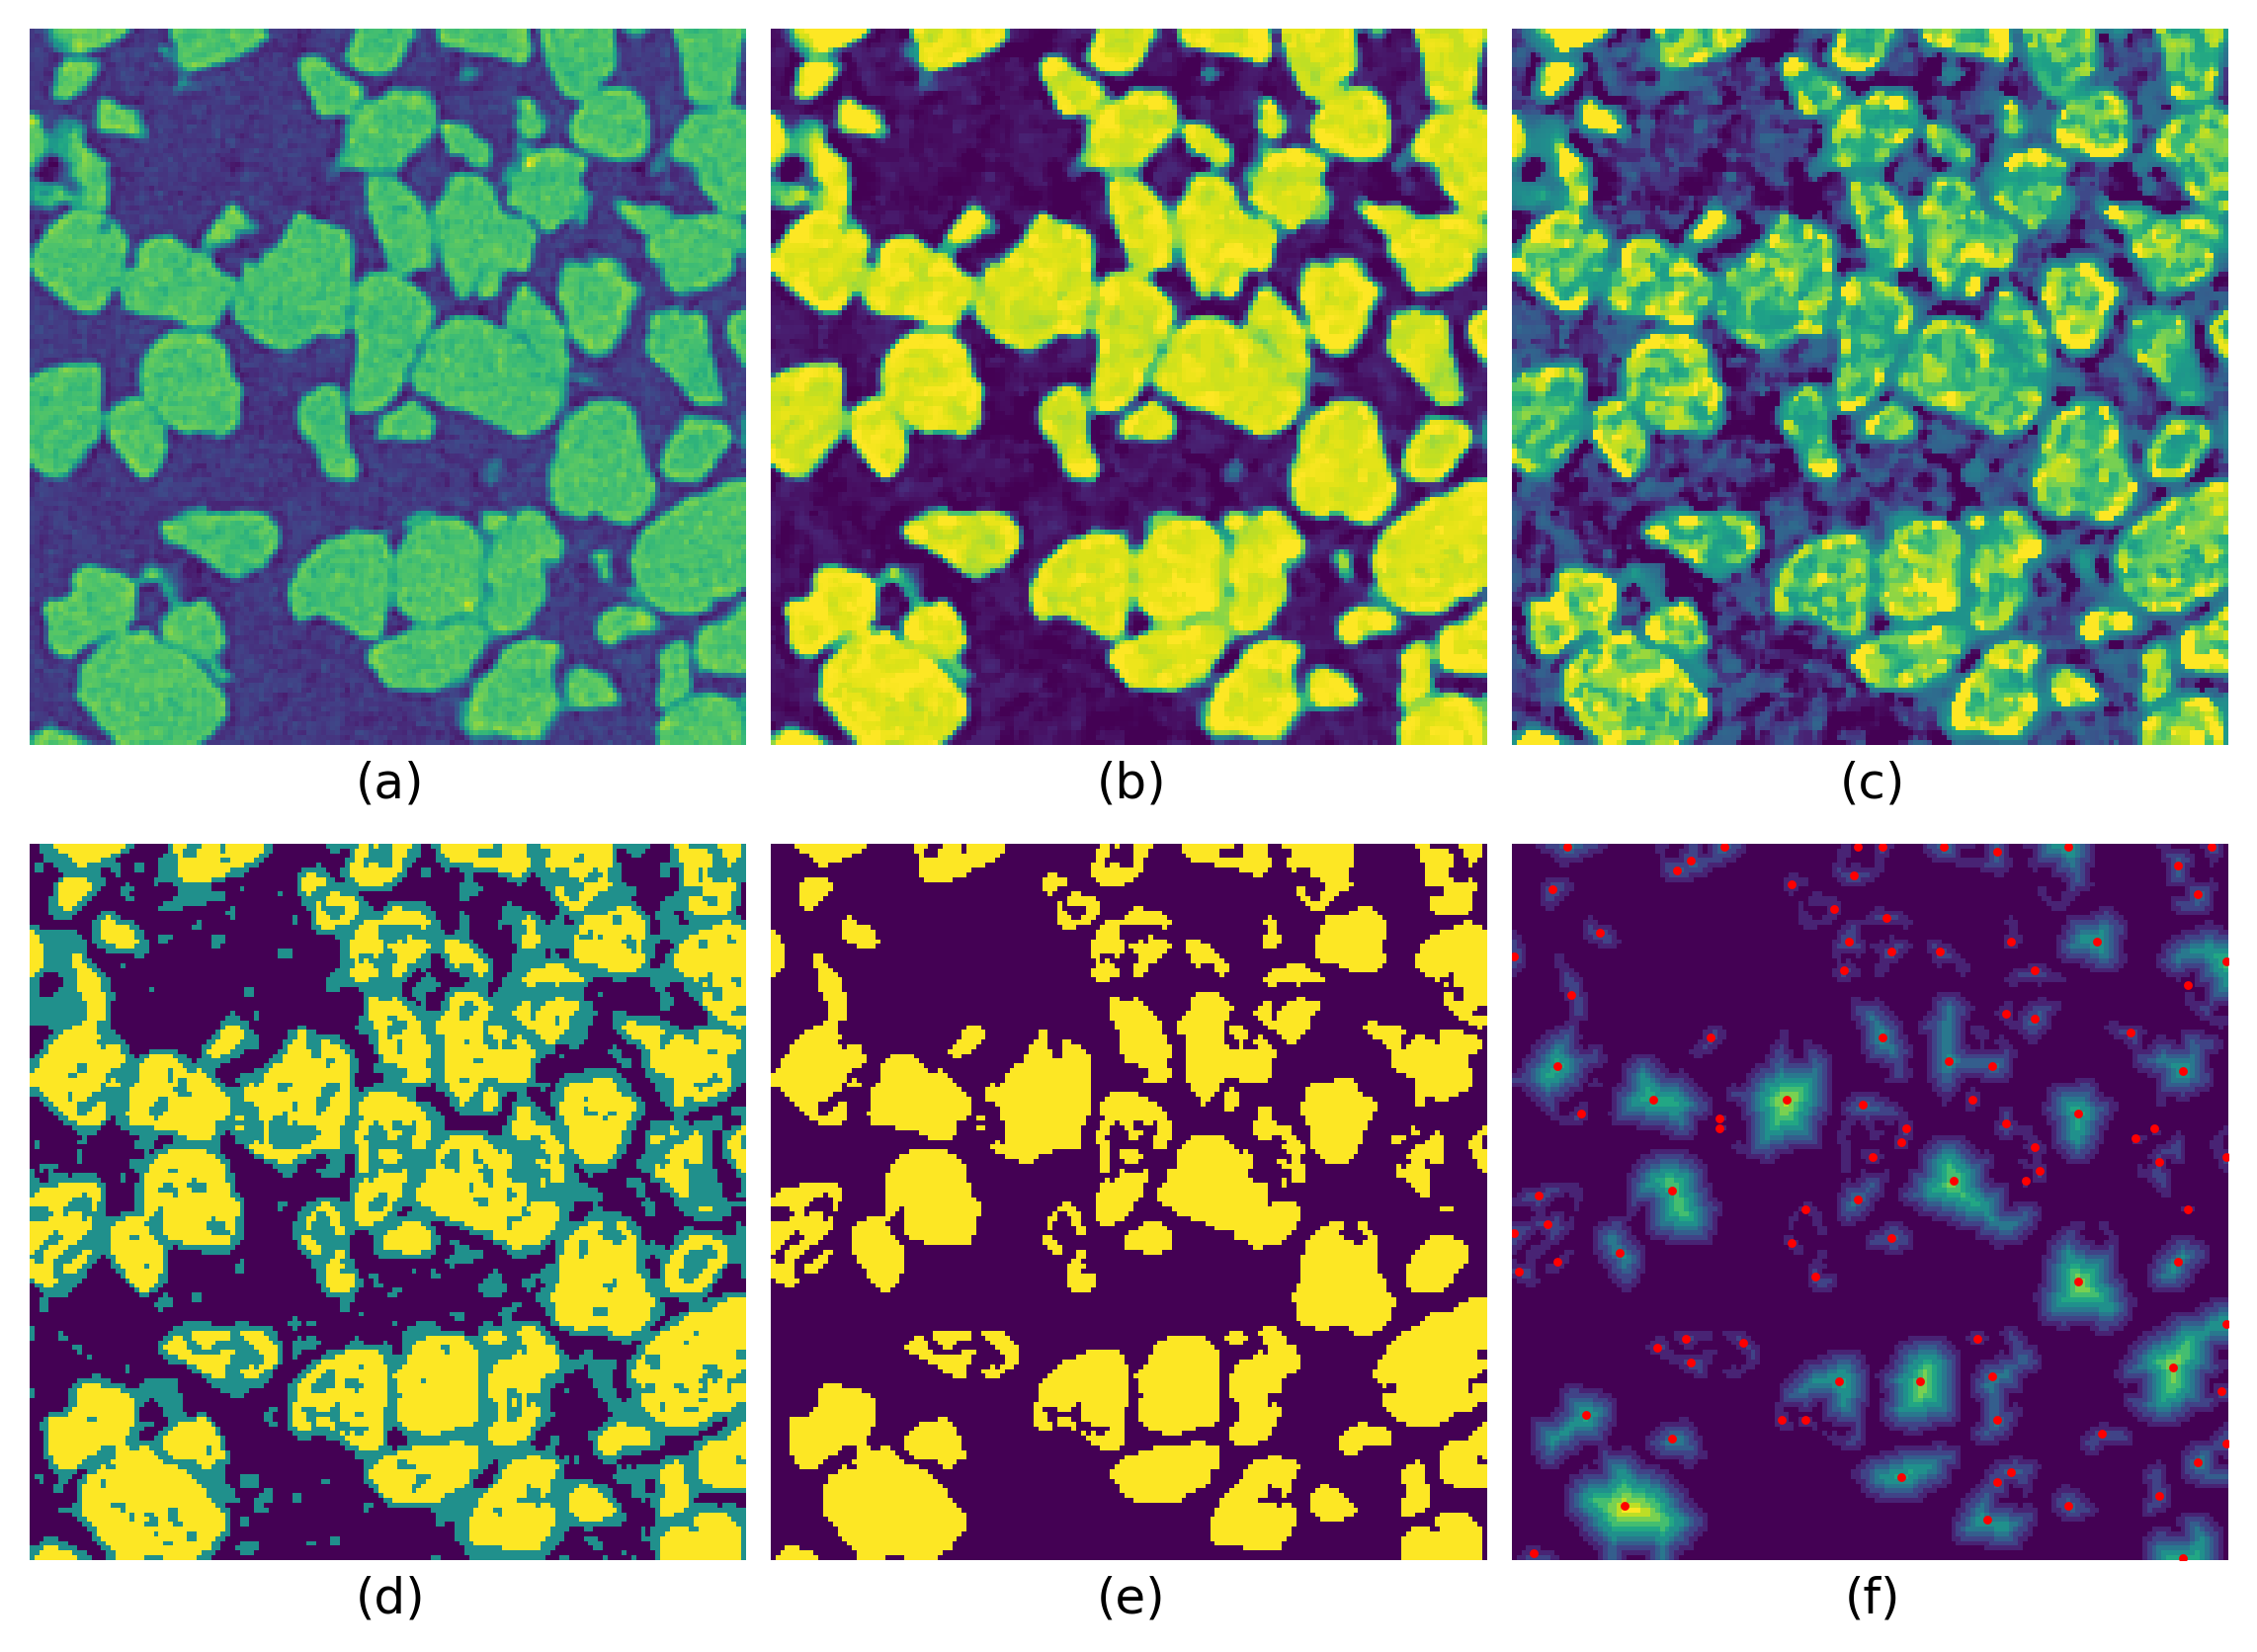
\includegraphics[width=0.75\textwidth]{figures/05/03-routine.png}
    \caption{
        \small\setstretch{1}
        (a) Image depicting sand grains sliced from a 3D CT scan.
        (b) Image rescaled to the range defined by the 5th and 95th percentile
        intensities.
        (c) Rescaled image after histogram equalization to enhance
        maxima within the particles.
        (d) Histogram-equalized image converted into
        a ternary image following application of a multi-Otsu algorithm with
        three classes.
        (e) Binary image created by thresholding the with uppermost value
        calculated by multi-Otsu algorithm. All holes within resulting regions
        of binary image are filled.
        (f) Euclidean distance transformation of multi-Otsu binary image with
        local maxima denoted by red points.
    }
    \label{fig/05/routine}
\end{figure}

% -------------------------------------------------------------------------
\subsubsection{Preparing Over-Segmentation}
% -------------------------------------------------------------------------
Before the local maxima markers are used to seed a watershed segmentation,
the markers are filtered such that any points close to a particle edge
in the image are removed. Over-segmented regions will be merged according
to edge strength between the markers, so having a marker lie on
an edge between two particles may prevent the edge from being detected. To
remove the markers closest to edges, an image is created that enhances the
intensity of particle edges by applying a Sobel filter, implemented in
\textit{scikit-image}, to the rescaled image (\ref{fig/05/edges}.b)
\cite{Kanopoulos1988}. In this image, the
strongest edges are represented by the highest intensities in the image.
The edges in the Sobel-filtered image are further emphasized by performing
adaptive histogram equalization from \textit{scikit-image}, which increases
the intensity of the weaker edges between particles.

\begin{figure}[ht]
    \centering
    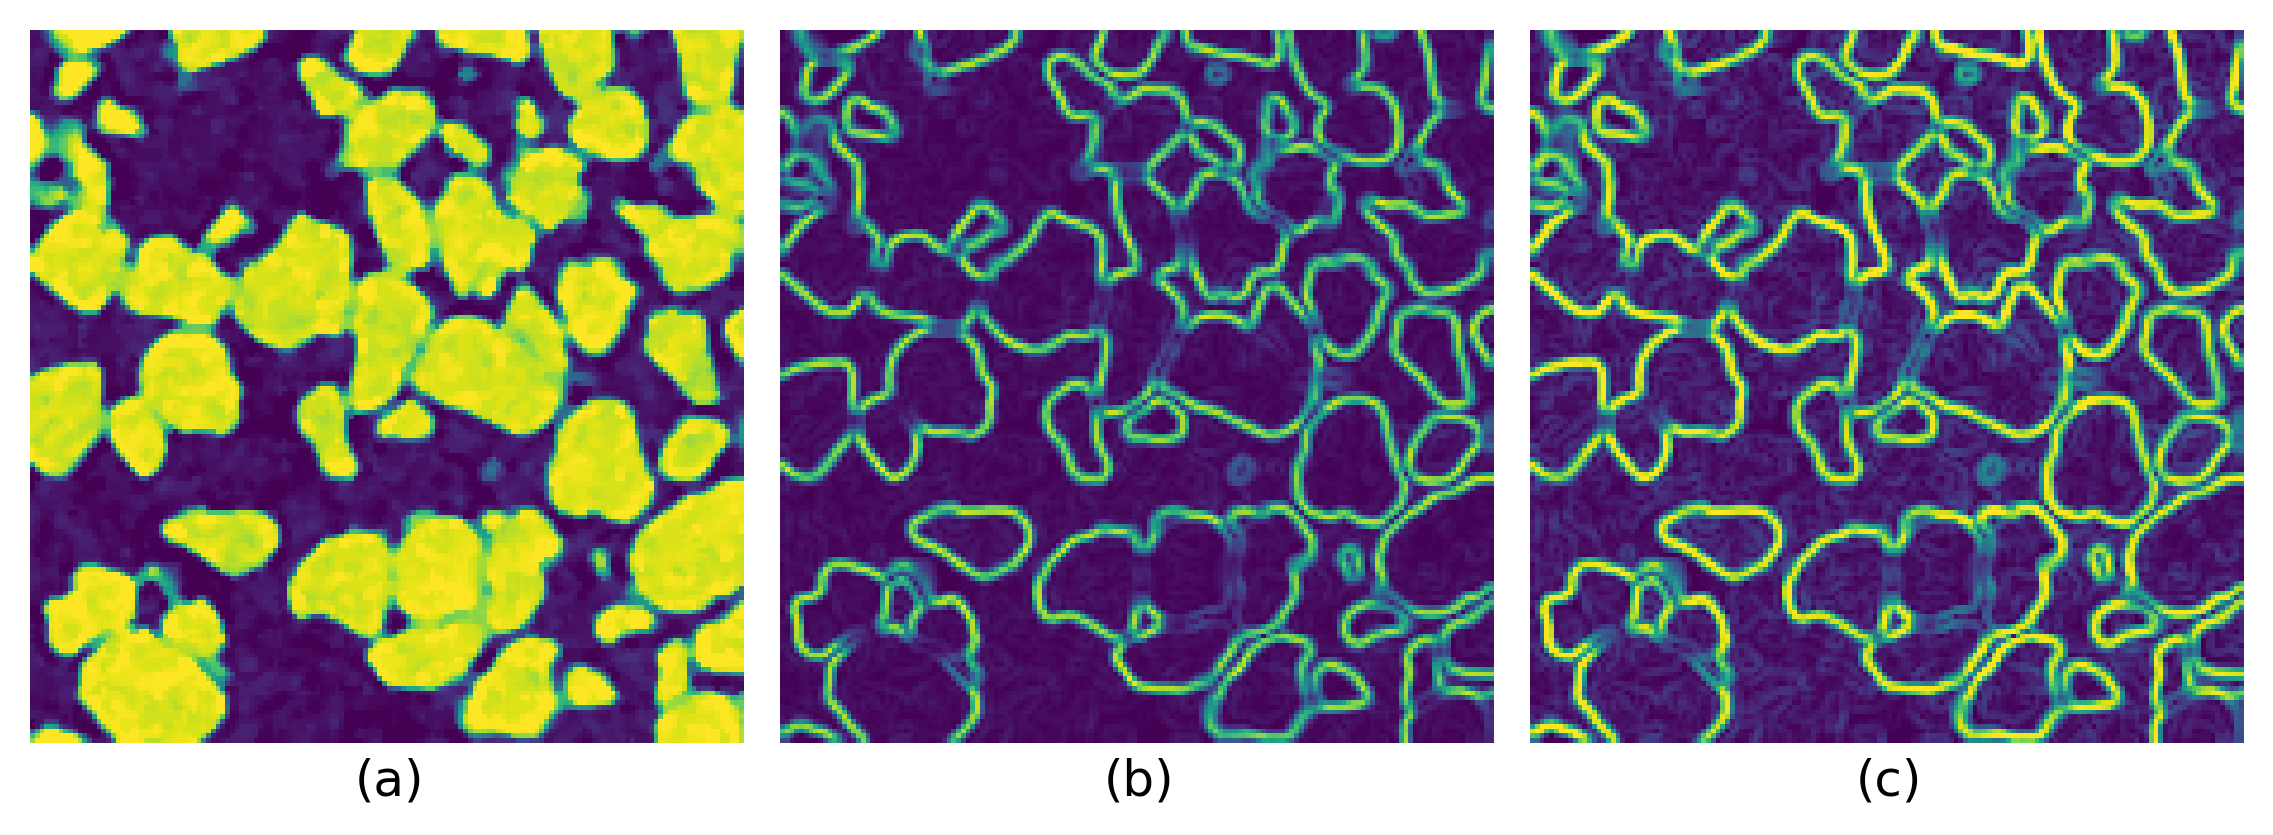
\includegraphics[width=0.75\textwidth]{figures/05/04-edges.png}
    \caption{
        \small\setstretch{1}
        (a) Rescaled image depicting sand grains
        (\ref{fig/05/routine}.b).
        (b) Rescaled image after application of a Sobel filter to enhance the
        edges of particles within the image.
        (c) Sobel-filtered image after adaptive histogram equalization is
        performed to further enhance particle edges.
    }
    \label{fig/05/edges}
\end{figure}

Sampling the intensity of the edge image (\ref{fig/05/edges}.c) at
the locations of
the inverse distance transformation minima, the points closest to the
edges will have the highest intensity. The points with intensities above
the 95th percentile are removed (\ref{fig/05/seeds}.b). The remaining
minima will be used as markers to seed the watershed segmentation.

\begin{figure}[ht]
    \centering
    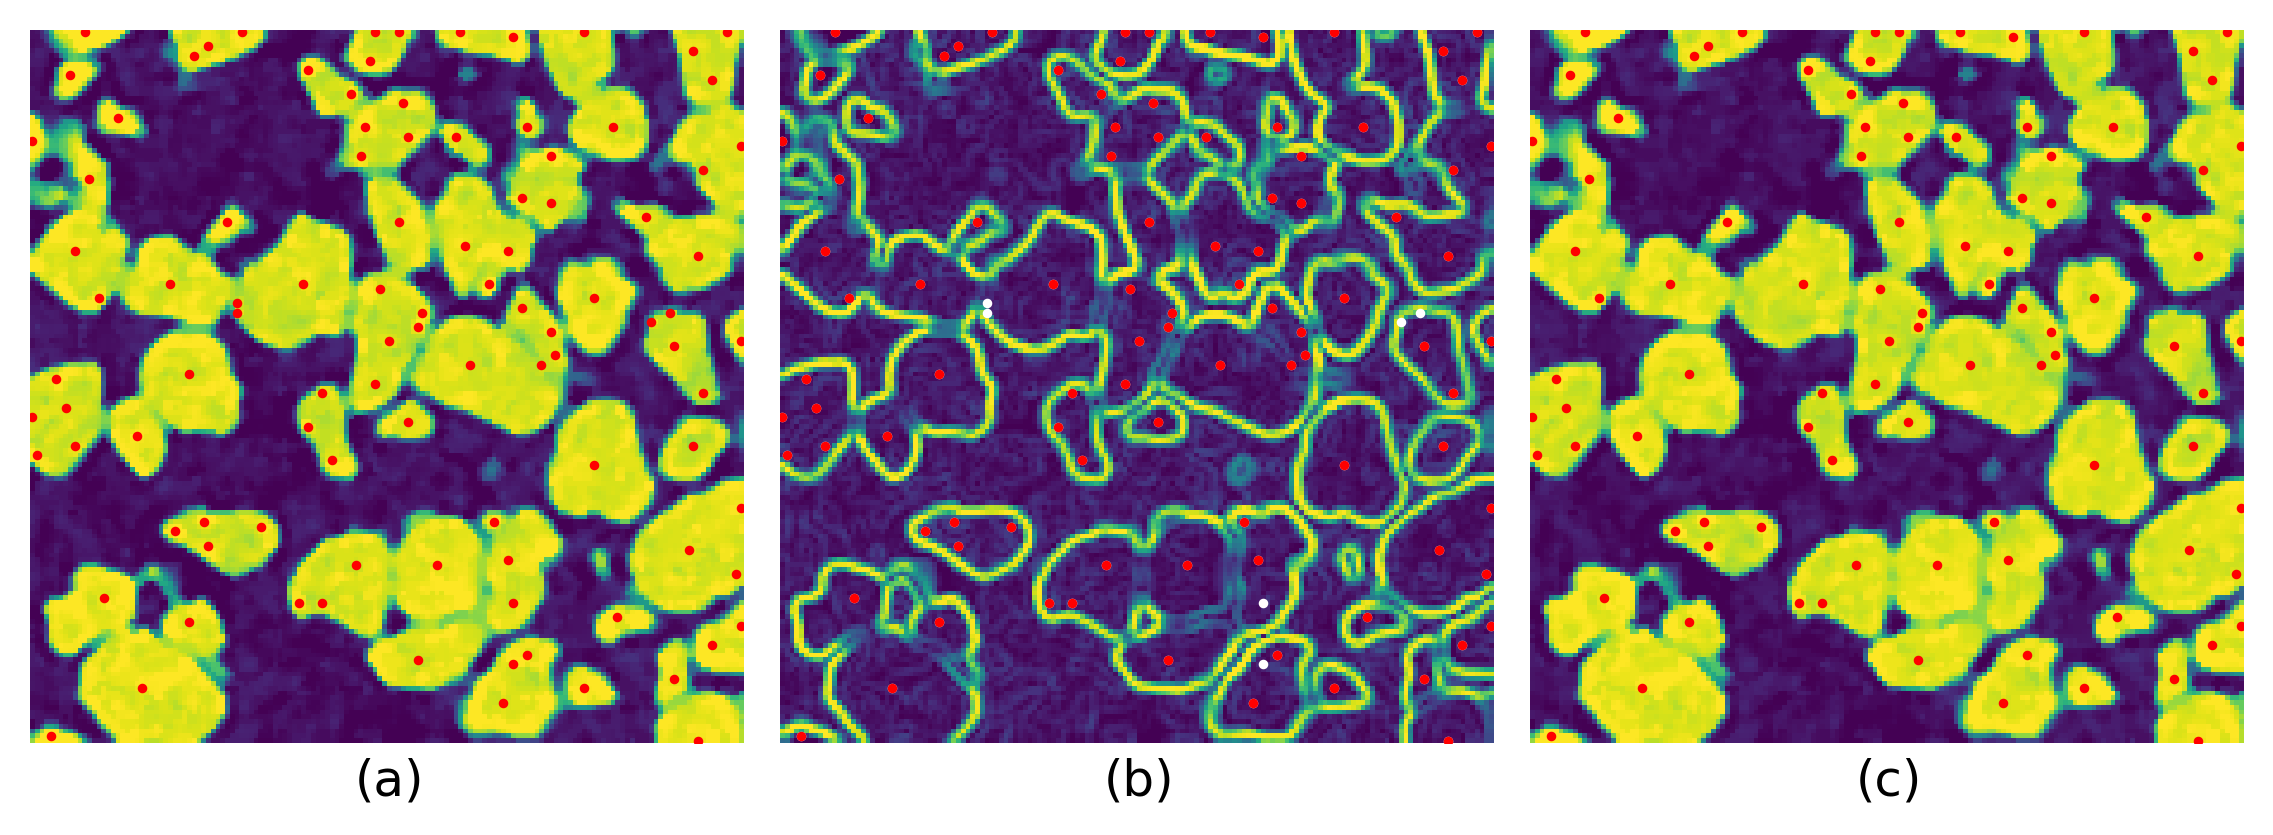
\includegraphics[width=0.75\textwidth]{figures/05/05-seeds.png}
    \caption{
        \small\setstretch{1}
        (a) Rescaled image depicting sand grains overlaid with
        inverted distance transformation minima in red.
        (b) Edge image (\ref{fig/05/edges}.c) with minima overlaid.
        White points are removed by filtering process for being too close
        to the particle edges while red points will be used as markers for
        the watershed segmentation.
        (c) Edge-filtered local minima (red) overlaid on the rescaled image.
    }
    \label{fig/05/seeds}
\end{figure}

The filtered markers seed a watershed segmentation operating on the
inverted distance transformation (\ref{fig/05/overseg}.b) created from
the multi-Otsu-binarized image (\ref{fig/05/routine}.e). Compared to the
visually discernible sand grains in the raw image (\ref{fig/05/overseg}.a),
the results of the watershed segmentation appear over-segmented as desired for
this stage of the procedure (\ref{fig/05/overseg}.c).

\begin{figure}[ht]
    \centering
    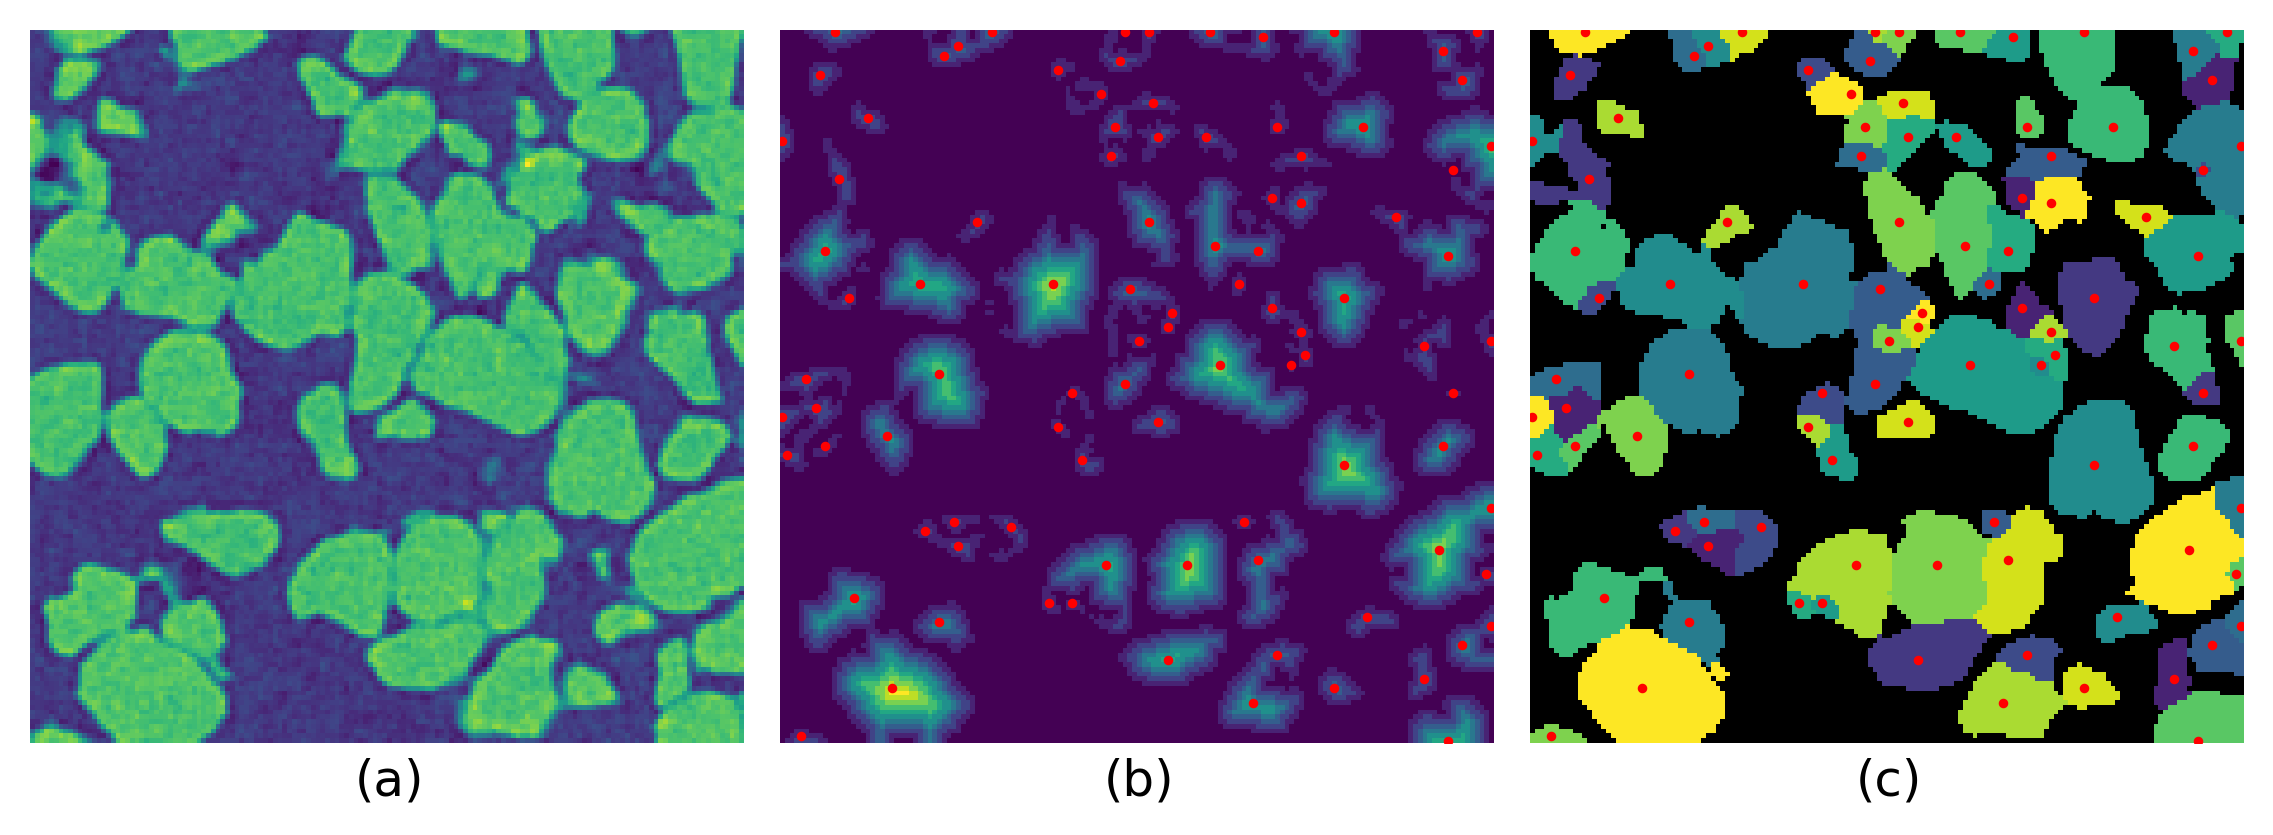
\includegraphics[width=0.75\textwidth]{figures/05/06-overseg.png}
    \caption{
        \small\setstretch{1}
        (a) Image depicting sand grains to be segmented.
        (b) Euclidean distance transformation of multi-Otsu-binarized image
        (\ref{fig/05/routine}.e) with edge-filtered local maxima denoted
        by red points.
        (c) Watershed segmentation results of the inverted Euclidean distance
        transformation seeded by the edge-filtered local maxima in previous
        image.
    }
    \label{fig/05/overseg}
\end{figure}

% -------------------------------------------------------------------------
\subsection{Delaunay Triangulation to Connect Markers and Detect Edges}
% -------------------------------------------------------------------------
A method has been developed to merge the over-segmented regions according
to edges detected in the vicinity of the regions.
Locations
between two regions determined to be neighbors must be searched for edges.
The regions will be merged if an edge is not detected between the two
regions. Before this can happen, however, a method is needed for
determining neighboring regions.
Each marker used to seed the segmentation will correspond
to one region, so the markers can be used to determine region neighbors,
but this process is still nontrivial.
As multi-sized markers will have neighbors at varying
distances, a method is needed that will connect each marker to its
neighboring markers without prior information about the distance to
those neighboring markers.
This can be achieved using Delaunay triangulation,
which calculates triangles between a distribution of points such that no
other points are within the circumcircle each triangle creates
\cite{Voronoi1908,Delaunay1934,Aurenhammer1991}.
The result is a structure that connects points with line segments of
varying lengths that do not overlap. Delaunay triangulation has been
applied to image segmentation before as an alternative method to watershed
segmentation. Wen et. al use Delaunay triangulation to segment clumps of
nuclei in cell-based fluorescent imaging \cite{Wen2009}.
In their method, points of
high curvature are detected in an image. These points are connected via
Delaunay triangulation and a geometry constraint is applied to the
triangulated lines to select the lines that separate the nuclei.
The method achieves results that align with expectations, however an
important requirement for this success is the consistently round shape
of the segmented nuclei such that
points of high curvature in the binary
image only occur at the points of contact between the particles.
Due to the irregular shape of the sand particles in the present work,
there are high points of curvature around the perimeter of single sand
grains, not only where the grains are in contact,
so this method would not be effective.
Instead of trying to use Delaunay
triangulation as a replacement for watershed segmentation, the routine
presented in this work uses Delaunay triangulation to
assist in merging over-segmented regions.

The neighbors of each marker are determined by calculating a
Delaunay triangulation with \textit{SciPy}, using the markers
corresponding to over-segmented regions (\ref{fig/05/delaunay}.a)
as the input vertices. The resulting
network of lines connect each marker to neighboring markers
(\ref{fig/05/delaunay}.b). This is useful in the
context of irregularly-shaped and multi-sized particles because the lines
connecting neighboring markers can be drastically different lengths.
Sampling the intensity of the edge image along each of these lines yields
intensity profiles, analysis of which is used to define the edge
detection. With a robust enough definition of a detected edge, edges can
even be detected between tightly-clustered sand grains. In this work,
an edge is defined as detected between two neighboring markers if the
maximum intensity along the line connecting the markers satisfies two
conditions: (1) the maximum intensity along the line must be greater than
10 percent of the edge image global maximum, and (2) the maximum
intensity along the line must not occur at either end of the line.
Most strongly defined
edges in the image are near the edge image global maximum, but the edge
detection definition must encompass a larger range of values to capture
the weakly defined edges which have a much lower intensity. Since this
edge detection value is so low, some lines that don't cross any edges are
falsely flagged as crossing an edge. This typically happens when one or
both markers at either end of the line are near particle edges, hence
the necessity of the second condition. The number
of falsely flagged edges is reduced by ignoring detected edges when the
maximum intensity of the line occurs at either endpoint. Markers that are
connected by lines on which edges are not detected are defined as
belonging in the same ``particle neighborhood'' and are merged in the
final stage of the procedure. The criteria used here for forming these
particle neighborhoods were
determined based on observation of the edges in this image and could be
tailored to specific experiments.

\begin{figure}[ht]
    \centering
    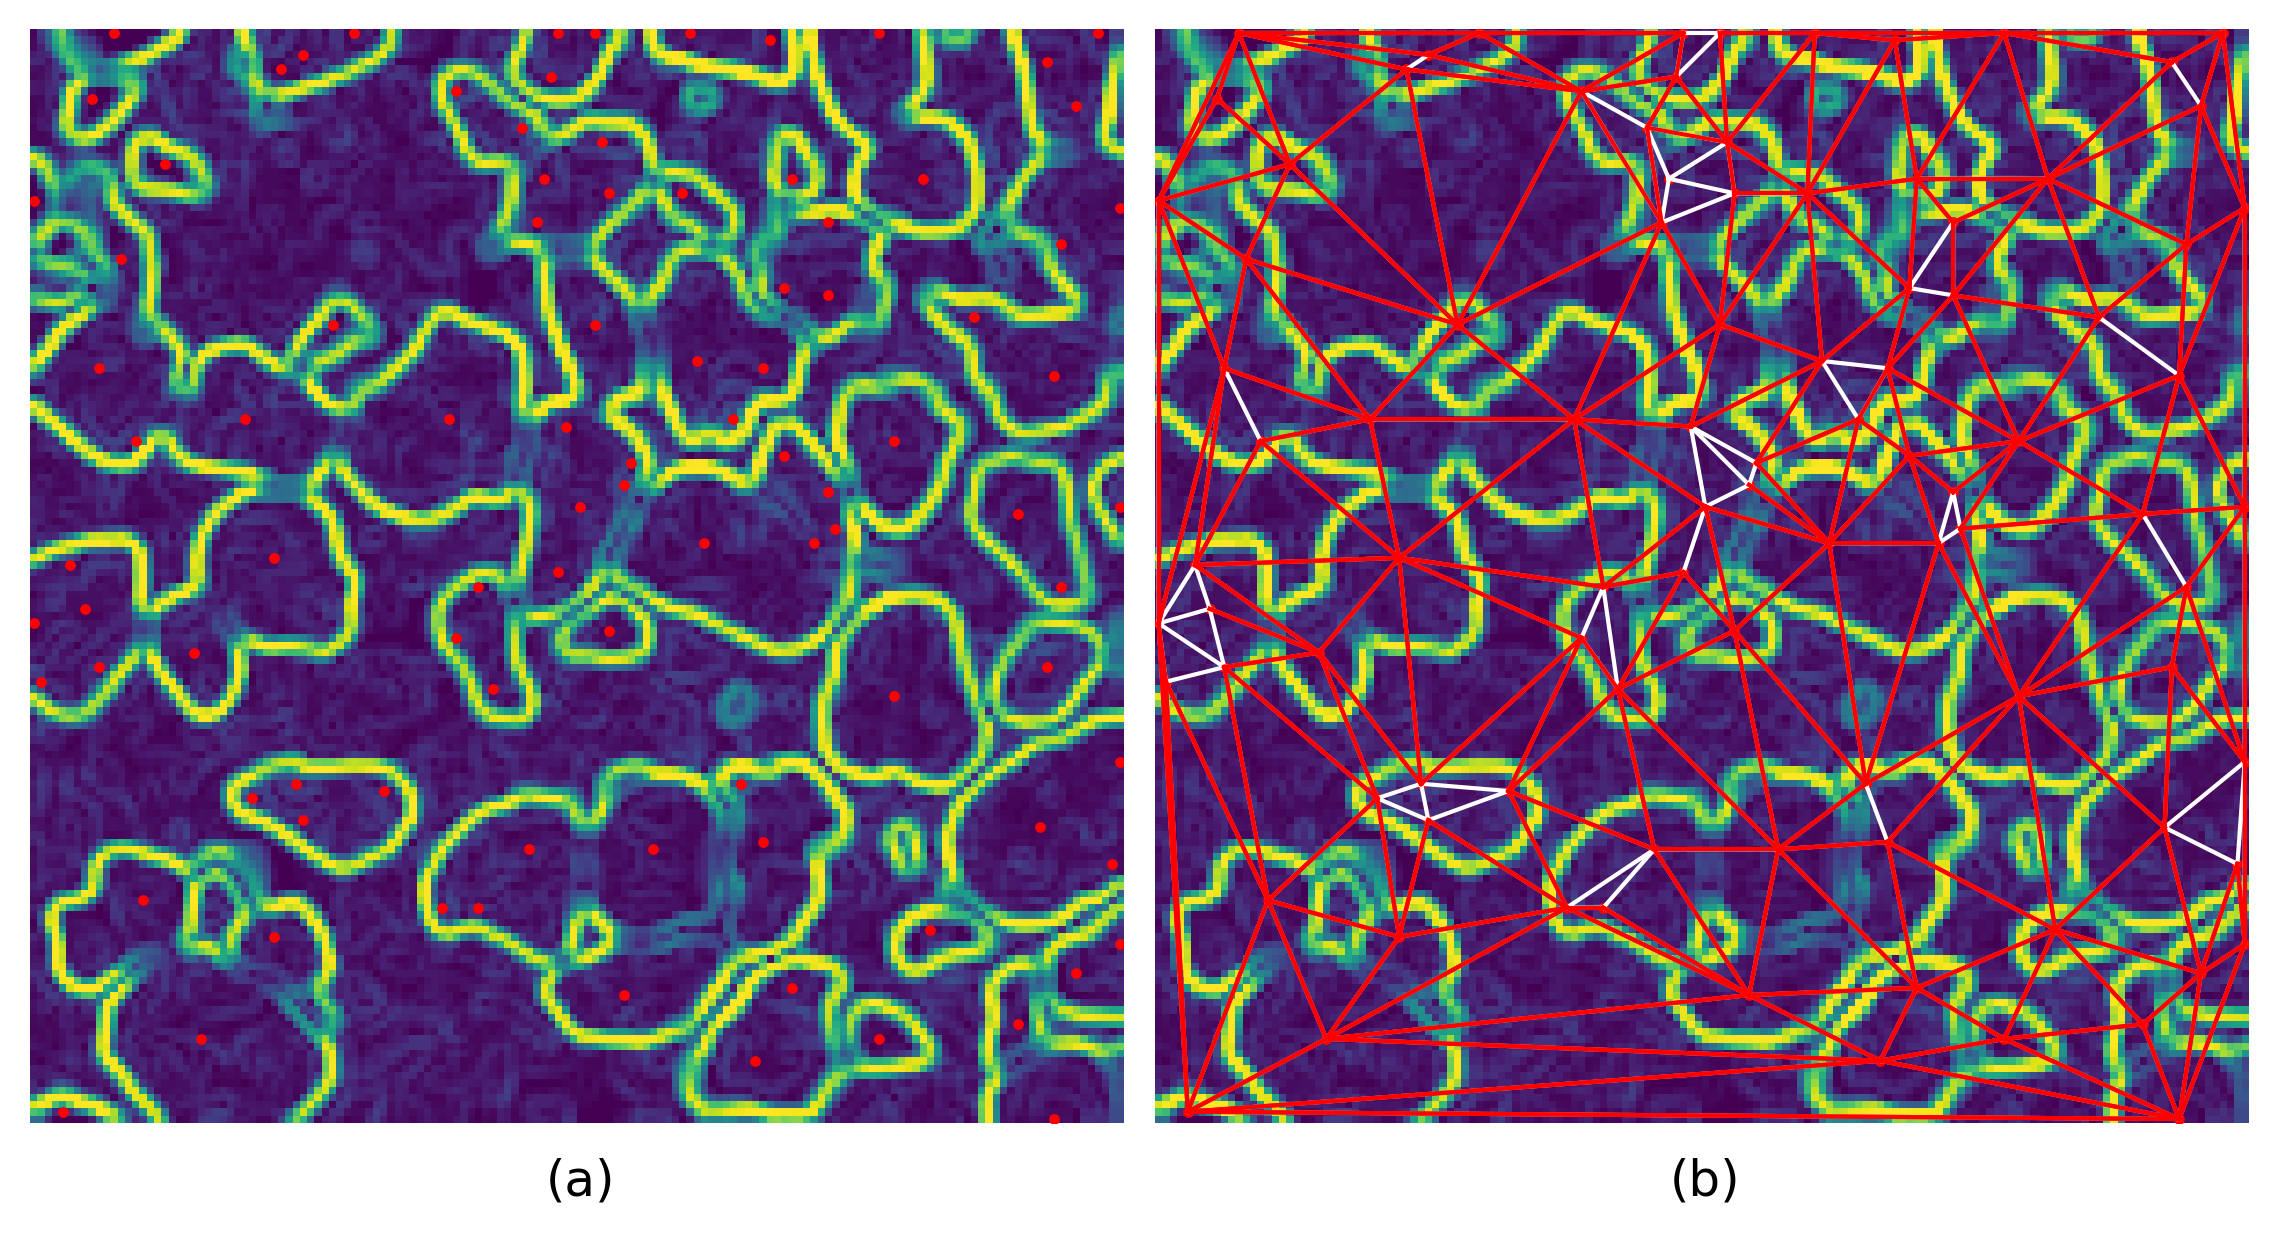
\includegraphics[width=0.75\textwidth]{figures/05/07-delaunay.png}
    \caption{
        \small\setstretch{1}
        (a) Edge-filtered maxima used as markers (red) overlaid on the
        edge image (\ref{fig/05/edges}.c).
        (b) Edge image overlaid with Delaunay
        triangulation. Red lines denote lines across which an edge was detected
        while white lines denote lines across which no edges were detected.
        Markers connected by white lines are defined as existing in the same
        ``particle neighborhood''.
    }
    \label{fig/05/delaunay}
\end{figure}


\subsection{Results}
% -------------------------------------------------------------------------
Particle neighborhoods created with the Delaunay edge detection algorithm
are used to correct the over-segmented results
(\ref{fig/05/merge-results}.b) obtained from the watershed
segmentation. The regions corresponding to each of the markers within a
particle neighborhood are merged such that each particle neighborhood has
only one associated region in the final segmented regions
(\ref{fig/05/merge-results}.c).

\begin{figure}[ht]
    \centering
    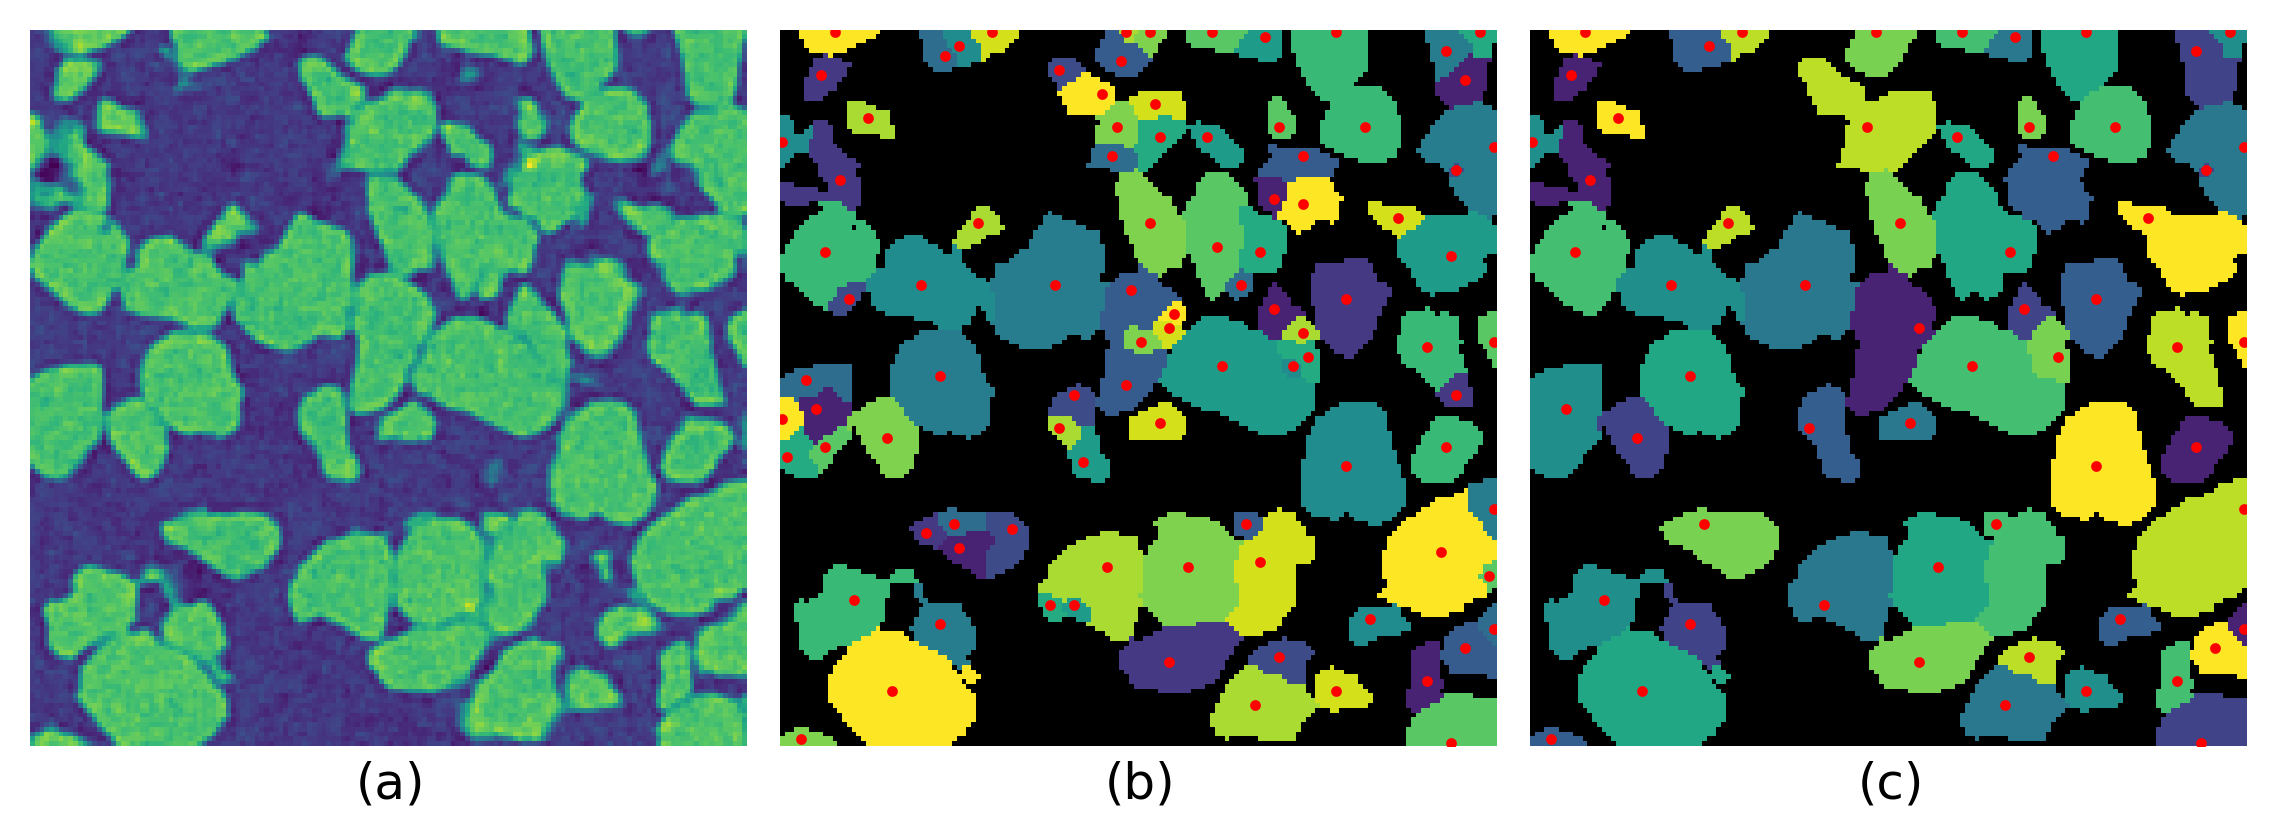
\includegraphics[width=0.75\textwidth]{figures/05/08-seg-results.png}
    \caption{
        \small\setstretch{1}
        (a) Image depicting sand particles to compare with segmentation
        results.
        (b) Over-segmented regions resulting from extended watershed routine,
        but before regions are merged (\ref{fig/05/overseg}.c).
        Red points correspond to marker used to segment the region.
        (c) Final segmented regions after merging neighboring regions without
        a separating edge (\ref{fig/05/delaunay}.b). Each red point
        corresponds to the marker of a merged region closest to the average
        location of all the centroids of the merged neighboring regions.
    }
    \label{fig/05/merge-results}
\end{figure}

The merging algorithm yields a segmentation that appears to more closely align with
expectations than the results from a typical watershed segmentation when
compared to the visually discernible grains in the original image
(\ref{fig/05/merge-results}.a). However,
in order to quantitatively determine the extent to which the merging algorithm
improves the results obtained from the watershed segmentation, the results from
the typical watershed and merged-region segmentations are compared to a manual
segmentation of the sand grains.
To generate the manual segmentation, a digital drawing application
with multi-layer functionality was used to individually draw the footprint of
each segmented grain on a separate layer overlaid on the raw image.
Each layer was then exported as a separate PNG image. These images were loaded into
Python using \textit{imageio} and \textit{NumPy}, and the grain in each
labeled image was assigned a unique integer ID using \textit{scikit-image}.

It is nontrivial to calculate the fit between two separate segmented images, even
though the images both represent the same system. Even when labeled regions are
relatively closely aligned, the labels in each segmented image will most likely not
match. To solve this problem, an algorithm was written to match the labels across two
separately segmented images based on maximum overlapping area without
reusing any labels. This allowed for a match value to be calculated by summing the
overlapping matching pixels and dividing by the sum of all pixels, matched and
mismatched. Using this method,
a match of 82.09\% was calculated between the manual segmentation and the
typical watershed segmentation,
whereas a match of 89.02\% was calculated between the manual
segmentation and the merged-region segmentation.


\subsection{Discussion}
% -------------------------------------------------------------------------
The novel segmentation method proposed in this work achieves segmented results
that are approximately 7\% more accurate than a typical watershed segmentation
when each are compared with the same manual segmentation.
AN overlay of the mismatched pixels can be used to visualize the improvements
between segmentations more clearly than a simple comparison.
Each segmentation is plotted with red pixels overlaid
indicating mismatched with the manual segmentation.
This visualization represents the higher number of mismatched pixels in the
typical watershed segmentation (\ref{fig/05/seg-comps}.c)
as a higher number of red pixels than in the merged-region segmentation
(\ref{fig/05/seg-comps}.f).

\begin{figure}[ht]
    \centering
    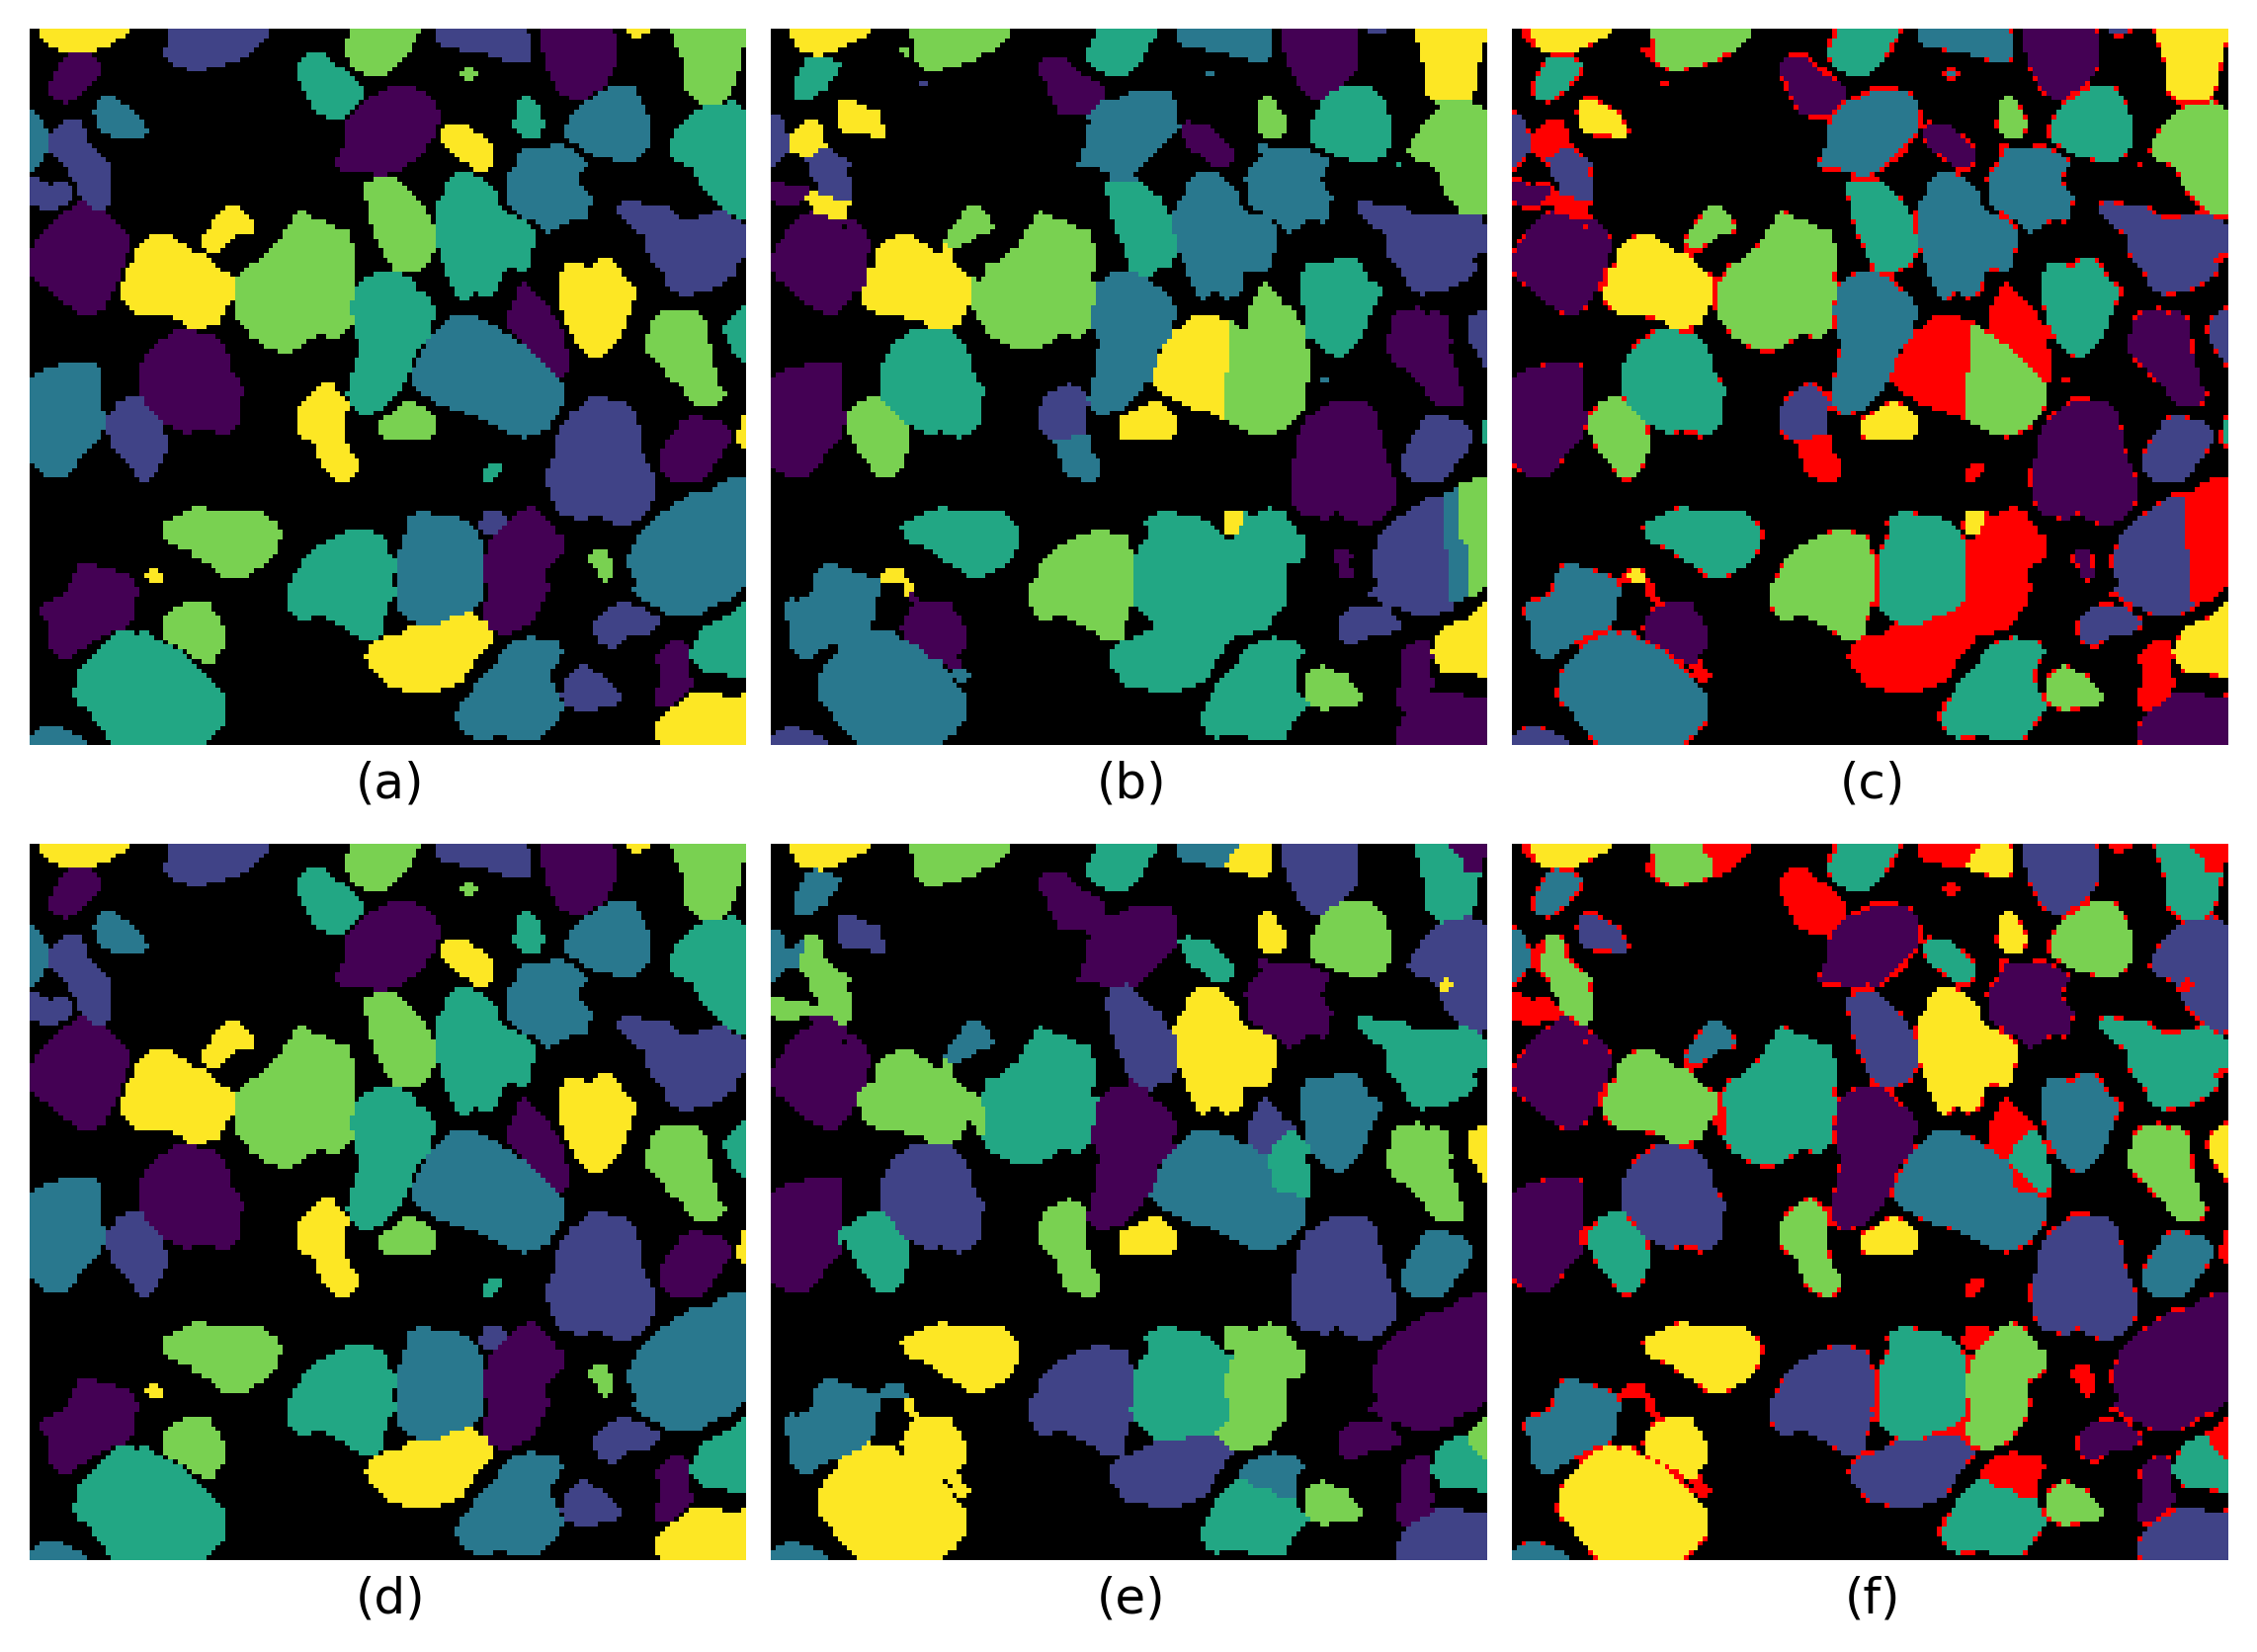
\includegraphics[width=0.75\textwidth]{figures/05/09-comps-to-manual.png}
    \caption{
        \small\setstretch{1}
        (a) Manual segmentation from hand drawing individual overlays
        on each visually discernible sand grain.
        (b) Typical watershed segmentation (\ref{fig/05/typical}).
        This segmentation achieves an 82.09\% match with the manual segmentation.
        (c) Watershed segmentation with red overlay depicting pixels mismatched
        from the manual segmentation.
        (d) Manual segmentation plotted again for ease of comparison with
        merged-region segmentation.
        (e) Merged-region segmentation from merging over-segmented
        neighboring regions without a separating edge
        (\ref{fig/05/merge-results}). This segmentation achieves an
        87.02\% match with the manual segmentation, approximately a 7\%
        improvement from the typical watershed segmentation.
        (f) Merged-region segmentation with red overlay depicting
        pixels mismatched from the manual segmentation.
    }
    \label{fig/05/seg-comps}
\end{figure}

The largest disagreement between the mismatch of the typical watershed
and merged-region segmentations is a cluster of sand grains at the bottom
center of each image. In the manual segmentation, the cluster is
identified as four large sand grains and one small sand grain. In the typical
watershed segmentation, the cluster is incorrectly identified as three sand
grains: the small sand grain, one large sand grain, and the final three large
sand grains identified as a single, larger grain. This is an example of
under-segmentation because the segmentation routine did not segment the sand
grains enough. The visualization of this
mismatch (\ref{fig/05/seg-comps}.c) also provides some insight to the
functioning of the mismatch calculation algorithm mentioned before, as the red
overlay classifies only two of the three large grains in the cluster as mismatched,
rather than all three. The third grain is classified as the matching portion of
the cluster because it is the largest constituent of the cluster and therefore
provides the highest number of overlapping pixels out of the three grains.
This same cluster of five particles is identified differently in the merged-region
segmentation. Each of the four large sand grains were
identified, but the small grain was identified as part of the rightmost
large sand grain. Even though the merged-region segmentation results are not
perfect for this cluster, misrepresenting the small sand grain results in
fewer mismatched pixels than the two larger mismatched grains in the typical
watershed segmentation.

The next largest mismatch disagreement between the typical
watershed and merged-region segmentation is a pair of tightly clustered sand
grains, one large and one medium sized, near the center of the image. In the
typical watershed segmentation, the grains are segmented into two regions, but
the segmentation occurs at the wrong location, leading to the entire small sand
grain identified as mismatching along with half of the large grain.
In the merged-region segmentation, the large sand grain is mostly segmented
correctly (aside from a small region near the boundary with the medium grain)
and the small sand grain is over-segmented into two regions instead of one.
Once again, the mismatch in the merged-region segmentation is less than that
of the typical watershed segmentation.

Another mismatch disagreement is in the segmentation of a large sand grain on the
lower right edge of the image. In the typical watershed segmentation, the grain
is over-segmented into three separate regions. The largest of these regions is
identified as matching with the manual segmentation, which leaves the two smaller
regions as mismatch. In the merged-region segmentation, the sand grain is correctly
identified as a single region. Contrasting this over-segmentation and directly below
this large grain in the bottom right corner is a pair of medium sand grains that are
improperly under-segmented as a single region in the typical watershed segmentation.
The two grains are segmented correctly in the merged-region segmentation, however,
with only a thin region of mismatch between the two grains.

Though the merged-region segmentation was calculated as more closely
matching the manual segmentation overall, there are still a few regions of
mismatch disagreement between the two segmentations where the typical watershed
routine yielded a segmentation that was closer to the manual segmentation
than the merged-region segmentation. The largest of these
regions is a pair of medium-sized grains in the top center of the image. While
these grains are properly segmented in the typical watershed segmentation, the
grains are under-segmented as a single region in the merged-region segmentation.
This leads to the smaller of these grains being identified as mismatching.
This kind of under-segmentation is also seen between a medium and small sand grain
in the upper left side of the merged-region segmentation, though this pair of sand
grains is also misrepresented in the typical watershed segmentation as four regions.
A similar example in which the merged-region segmentation under-segmented a small
sand grain occurred for a small sand grain between two larger grains in the bottom
left corner of the image. The sand grain was segmented separately in the typical
watershed segmentation, though even in that segmentation the surrounding
area was still identified as mismatching in a way reminiscent of the
merged-region segmentation.

There are also a few cases of over-segmented grains in the merged-region
segmentation that are not present in the typical watershed segmentation. The
largest of these is a medium sand grain in the bottom center of the image that
was improperly segmented into two regions. The rest of the over-segmented regions
in the merged-region segmentation (besides the over-segmentation of the smaller of
two tightly clustered sand grains previously mentioned) are around the edges of the
image (e.g., top left edge, top right edge, top right corner, bottom right edge).
These over-segmented regions are all rather small, so they don't contribute much to
the overall mismatch with the manual segmentation, but their presence raises the
question of whether this algorithm would be even more successful if it was applied
to an image that contained only complete particles not split by image borders.

The last features to note in these images are the portion of the red overlays
corresponding to thin regions around the edge of some sand grains. These pixels
correspond to small regions of mismatch where the footprints of the manual and
typical/merged-region segmentations do not agree. These mismatched areas are present
because both the typical watershed and merged-region segmentations require a semantic
segmentation step to create a binary image differentiating particles from background.
From this binary image, markers are generated and passed to the instance segmentation
portion of the routines to segment and label the individual particles. This process
is mostly the same for the typical watershed and merged-region segmentation, resulting in
similarly mismatched regions along the edges of the particles where the
semantic segmentation slightly differs from the footprint of the manual segmentation.
The reason these regions are only mostly the same for these segmentations is because the
process of selecting markers from each semantic segmentation is slightly different in the
merged-region segmentation versus the typical watershed, as described previously. This leads
to some of the smallest sand grains not receiving a marker in one segmentation, but receiving
a marker in the other, leading to discrepancies in the mismatch.
Regardless, these regions are small, so
their contributions to the larger mismatch of the image are minimal.


\subsection{Conclusions}
This work presented a procedure to improve the segmentation of
irregularly-shaped, multi-sized, and tightly-clustered particles
using a method that merges regions based on edge strength.
A 2D image taken from a 3D XCT scan of polymer-bonded sand grains was
used as an example image. The procedure preprocesses the image to
create a binary image separating the sand grains from the background and
generates a set of markers to intentionally over-segment the particles.
The majority of the procedure lies in a custom algorithm which utilizes
Delaunay triangulation to merge neighboring regions that are not found to
be separated by an edge.

The merged-region segmentation appears to be an improvement over a typical
watershed segmentation, however a manual segmentation was also performed
and used as a baseline to quantitatively assess the improvement.
The fit between the manual segmentation and merged-region segmentation is
calculated and compared to the fit between the same manual segmentation
and the typical watershed segmentation.
The merged-region segmentation was calculated to be an 89.02\% fit with
the manual segmentation. This is a 6.93\% improvement over the typical
watershed segmentation, which was calculated to be an 82.09\% fit with the
same manual segmentation.



% -------------------------------------------------------------------------
%   Chapter 6
% -------------------------------------------------------------------------
\newpage
\chapter{
    SEGMENTFLOW: A SEGMENTATION WORKFLOW PACKAGE FOR CREATING
    SIMULATION-READY GEOMETRIES FROM 3D IMAGE DATA} \label{ch/sf}
% 6.1 abstract
% \section{Abstract}
This chapter presents \textit{Segmentflow}, a segmentation workflow tool
that can be used to generate geometries for use in image-based
physics simulations.
The capabilities of \textit{Segmentflow} are demonstrated
by presenting the process of creating surface meshes
from a CT scan of a mock high explosives system consisting of tens of
thousands of F50 sand grains coated in a Kel-F polymeric binder.
Segmented particles are produced from segmentations seeded in five different
ways. Each segmentation is analyzed to assess the accuracy compared to
typical F50 sand.
Surface meshes are created from the segmented particles resulting from
the segmentation with the lowest error. An example surface mesh is subject to
a variety of postprocessing and the resulting surfaces are compared.
This postprocessing exhibits the important ability of\textit{Segmentflow}
to control the complexity that geometry introduces to simulations.


% 5.1 Introduction
\subsection{Introduction}
\textit{Segmentflow} is a Python package for creating segmentation
workflows which
convert 3D image data to a format usable in image-based simulations.
This software has been designed to be flexible enough
to be used for a variety of applications and data types. Part of what
makes \textit{Segmentflow} flexible is the ability to tune the segmentation
process and the format of the resulting outputs.

\textit{Segmentflow} was designed
to extract the geometries of granular particles embedded
in a polymeric matrix for image-based simulations.
Specifically, the behavior of these particles would be simulated in
quasi-static, unconfined compression by performing a
direct numerical simulation (DNS) on the real geometries
extracted with \textit{Segmentflow}.
These samples are imaged using x-ray computed tomography (XCT).
For the granular particles, the goal of the segmentation is to separate
each particle from the other particles and the polymeric binder,
then to convert the grayscale intensity voxel data to
a labeled voxel format and a collection of surface meshes
(one surface mesh for each particle).
Each of these output types would be
used as inputs for a different type of simulation software.

\textit{Segmentflow} ties together the functionality from many powerful
Python libraries. To improve make interfacing with \textit{Segmentflow}
more user-friendly, YAML files are used to pass input parameters to
\textit{Segmentflow} functions using the package \textit{PyYAML} \cite{pyyaml}.
To load and save images, the package \textit{imageio} \cite{imageio}.
Image data and manipulations are performed using \textit{NumPy} arrays
\cite{numpy}. Viewing images and plotting data and information about these
images is accomplished with \textit{Matplotlib} \cite{matplotlib}.
Many useful image processing algorithms implemented in
\textit{scikit-image} are utilized \cite{skimage}. To save surface meshes
in the STL file format, the package \textit{numpy-stl} is used \cite{numpystl}.
Finally, image postprocessing methods as well as 3D visualization rely on
the powerful 3D data processing library \textit{Open3D} \cite{Zhou2018}.

There are two types of segmentation, and the distinction between these types
is important for \textit{Segmentflow} because many segmentation workflows
depend on both types.
The first type of segmentation, semantic segmentation, is the process of
separating, or segmenting, features in an image by type or class.
Semantic segmentation on its own can be useful to determine information
like volume fractions, but often a semantic segmentation is the first step
for a more involved analysis.
There are different methods for performing semantic segmentation,
often by setting a series of threshold values in an image
and classifying features between those values.
This can be done manually or procedurally. A common algorithm for
procedurally determining threshold values is
known as multi-Otsu thresholding \cite{Otsu1979}.
The second type of segmentation is instance segmentation.
In instance segmentation, a region/class of an image,
is segmented into individual feature
instances, or segmented particles, of that class.
Often instance segmentation operates on a binary
representation of a class previously determined via semantic segmentation.
These segmented particles will be identified via labeled
voxels in which each voxel corresponding to a unique particle will be
labeled with a unique integer.

A common type of instance segmentation
is watershed segmentation.
Watershed segmentation can be
thought of as a simulated flooding process applied to an image
\cite{Beucher1979,Beucher1992,Soille1990viscomm,Soille1990sigproc,Vincent1991}.
As a watershed algorithm is applied to an image, the intensities of the
image act as elevations of a topographic surface. Simulated ``water'' can be
filled from the lowest elevations first, equal across the full image,
or the water can be ``poured'' from specifically locations called markers
\cite{Moga1998,Parvati2008}. As the water fills the surface,
separate ``catchment basins'' regions that started filling in different
places begin to near one another. Any time two catchment basins come into
contact, a ``dam'' is created. The algorithm finished when the image a has
been completely filled, or reaches a specified elevation/intensity. The
resulting dams denote the segmented regions.
It is common for watershed segmentation to be
applied to a distance transformation of a binary image, which in the case
of the Euclidean distance transformation (EDT), assigns a new
value to each foreground pixel according to the distance to the nearest
background pixel \cite{Danielsson1980}. This creates an image that is more
logically akin to an elevation map, as the distance map has a natural
gradient. The distance transform of a few black spots on a white image
would appear as a mountainous island, with the peak of the island at the
farthest point from the shore of the metaphoric white sea. If the distance map
is inverted, a gradual depression is formed that can be filled by the
algorithmic flooding using information about the morphology of the
foreground region in an image to segment the features.


% 6.2 Methods
\subsection{Methods}
To demonstrate the capabilities of \textit{Segmentflow},
a full CT scan to simulation geometry workflow is demonstrated on a
mock high explosives system
consisting of F50 sand grains coated in a polymeric Kel-F binder.
The sand was coated with the binder and pressed into a cylindrical
sample. The goal of the workflow is to create segment the sand grains from
the binder and create a series of surface meshes representing each of the
tens of thousands of sand grains in the sample such that the surface mesh
representation of the sample could be loaded into a simulation software as
an initial condition for physics simulations, such as deformation.
This demonstration uses \textit{Segmentflow} to load parameters from an
input file, preprocess the CT scan images to improve the contrast, perform
a semantic segmentation to identify the sand grains, create a surface mesh
for each segmented particle and save that mesh as an STL file, and finally
postprocess the surface meshes to change the properties of the meshes.
Though this work mainly focuses on the workflow for this particular material
system and application, alternative functionality is presented throughout
the demonstration to show how the workflow and parameters might be adapted
to other systems.

\subsubsection{Input Handling}
% -------------------------------------------------------------------------
\textit{Segmentflow} was designed to create simulation-ready geometries for
a wide range of applications, so a parameter specification system is
important to tune the various algorithms the packaged leverages to segment
a specific dataset. Since \textit{Segmentflow} is a Python package, it can
easily be installed so that the functions within may be imported into other
Python scripts. However, to make \textit{Segmentflow} more user friendly,
it was structured such that it could be operated by workflow scripts. Each
script is tailored to a specific workflow and has its own accompanying input
loading function that pulls parameters from an input file in YAML format.
This allows parameters to be
listed quickly and easily with text in a human-readable way while also
listing out the potential parameters that can be adjusted without having
to dig through documentation to know what can be changed. The YAML file
format has the added benefit of allowing parameters to be grouped together.
For the \textit{Segmentflow} input file, the grouping was made according
to the section of application the parameter affects.
Grouping makes tuning segmentation behavior more clear for the user
while also improving code readability because parameters loaded into
\textit{Segmentflow} are stored in
a nested dictionary according to these groups. In an effort to further improve
accessibility, any parameters in input files are able to be left
blank to set parameters to the default value.
This allows users to use \textit{Segmentflow} even if
they are unfamiliar with the parameters. Parameter specification using an input
file makes the segmentation routine reproducible because \textit{Segmentflow}
can be executed with the same input file multiple times to achieve the same
results. A copy of the input file is
also saved to the output directory specified in the input file for two
reasons: to backfill
default values that may have been filled for empty parameters and to store
a record of segmentation parameters to preserve
reproducibility in case the original input file is altered.

\subsubsection{Preprocessing}
Image preprocessing is the portion of the F50 sand segmentation procedure
involves loading the raw 3D data and performing operations to improve the
contrast. The location of the directory as well as
the image file format are specified in the input file.
With the images loaded, the
next step of the preprocessing routine is to perform a series of steps, as
specified in the input file, to improve the contrast of the images. In the
F50 sand procedure, a median filter is applied to the CT scan
to replace each voxel with the median value of the surrounding cube
of voxels, reducing localized noise while maintaining the sharpness of
edges (unlike Gaussian filtering which will blur edges).
Intensity clipping is also performed to improve contrast by taking advantage
of the full range of available intensities according to the image data type.
This is done by providing an upper and lower percentile interval in the
input file. The range used to rescale the F50 sand sample was [0, 99.9].

\subsubsection{Semantic Segmentation}
% -------------------------------------------------------------------------
In the F50 sand sample, the classes that exist within the images are
void, particle and binder.
\textit{Segmentflow}
uses an implementation of this algorithm \textit{scikit-image}.
Multi-Otsu thresholding divides an
image into \textit{N} classes based on the distribution of intensities in
an image by maximizing inter-class variance. To make \textit{Segmentflow}
more flexible, \textit{N} is included as an
input file parameter for some workflow scripts.
\textit{Segmentflow} also includes a custom thresholding algorithm that
uses a Gaussian filter to smooth the histogram of the 3D image, calculate the
local maxima corresponding to the peak intensity relating to the three
feature classes in images (void, binder, and sand grain). Minima are found
between each of the maxima and used as the threshold values
(\ref{fig/06/thresh}).

\begin{figure}[ht]
    \centering
    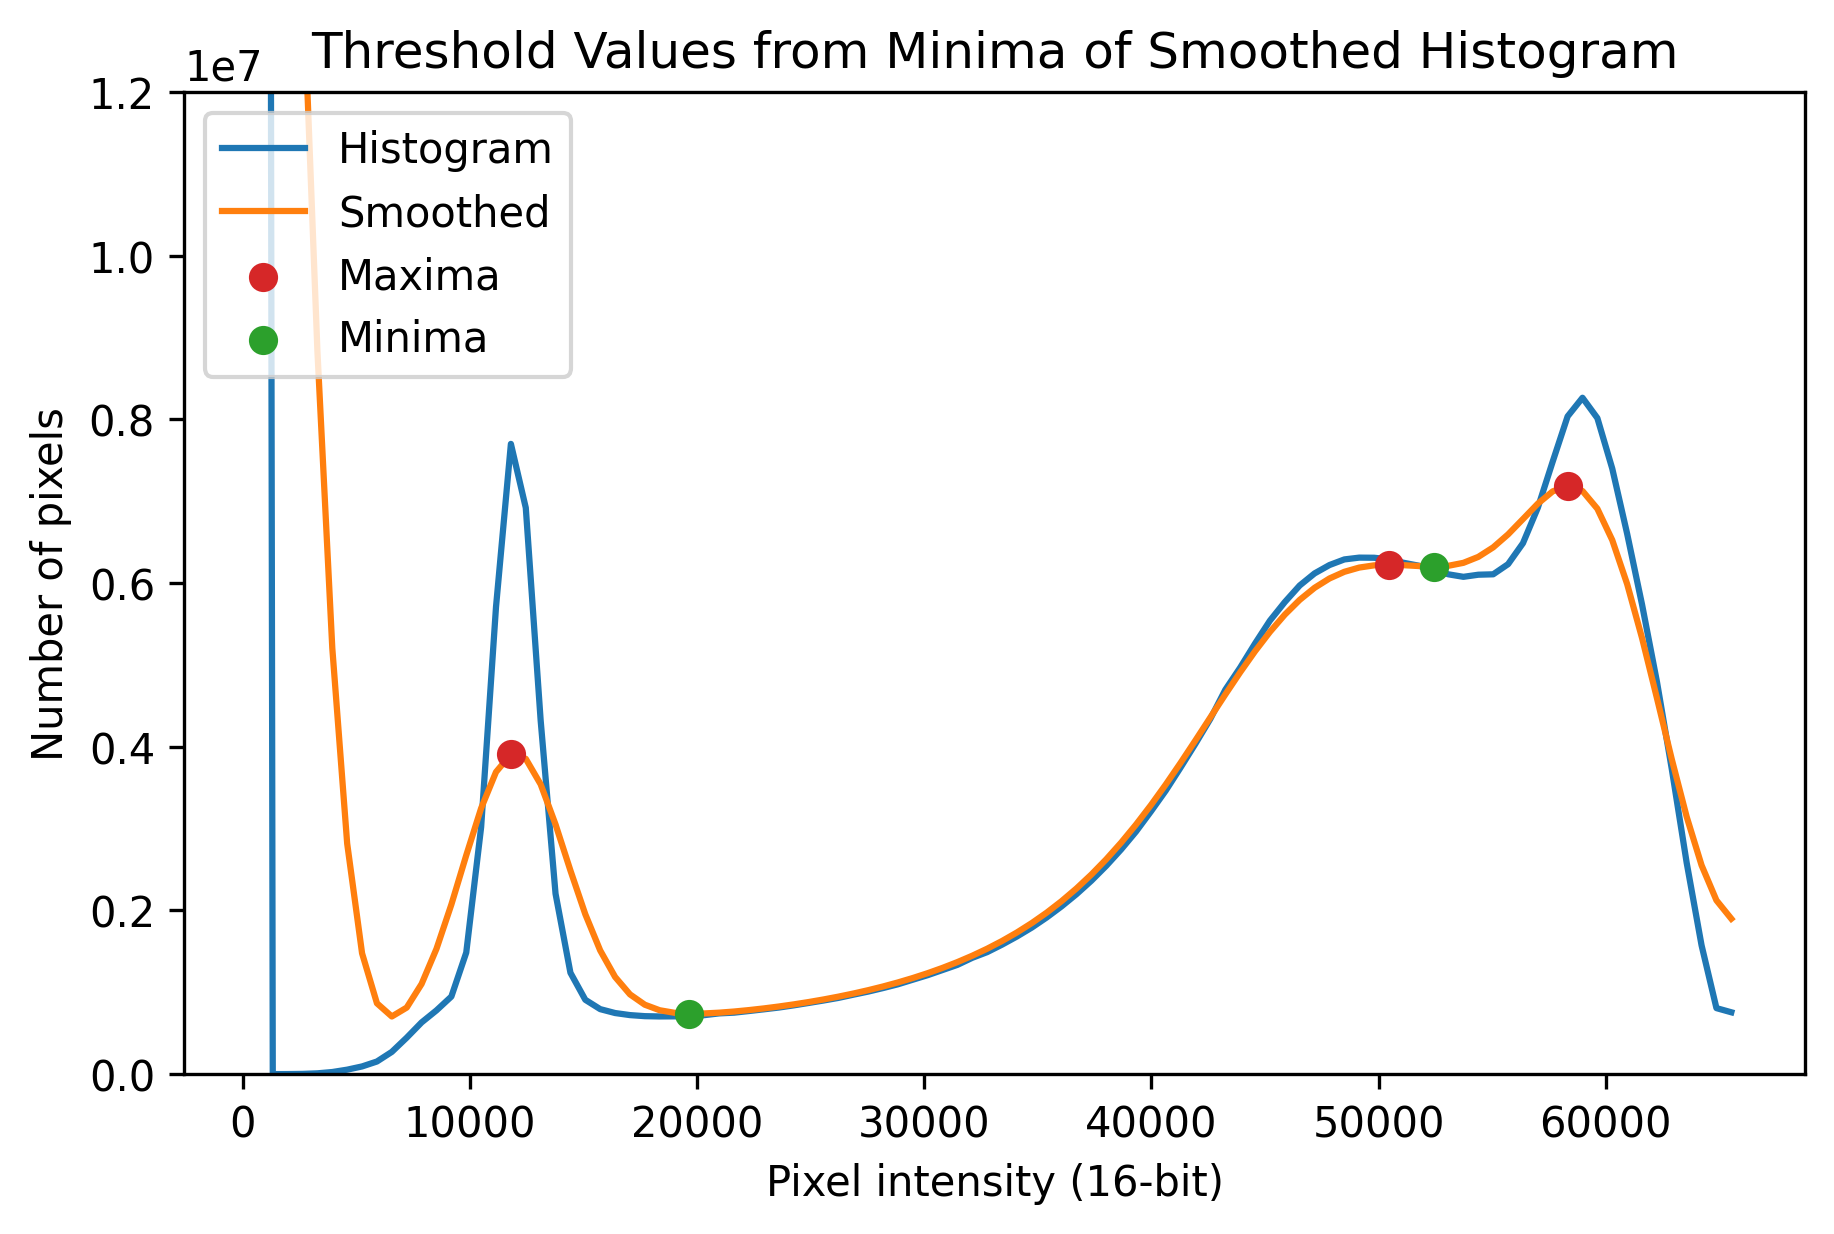
\includegraphics[width=0.75\textwidth]{figures/06/01-multi-min-hist.png}
    \caption{
        \small\setstretch{1}
        Histogram processing used to determine the threshold values to
        perform semantic segmentation on images. The blue line represents the
        raw histogram. The orange line represents the smoothed histogram.
        The red points denote the local maxima. The green points denote
        the local minima between these maxima which are used to threshold the
        material classes.
    }
    \label{fig/06/thresh}
\end{figure}

If this is a sufficient amount of segmentation
for the given application, \textit{Segmentflow}
can save a voxel representation of
the classes without undergoing further segmentation of the foreground. If
this option is specified in an input file, each voxel of a class is
represented by a unique integer label and saved as a collection of 2D
images. Otherwise, after dividing the image into \textit{N} classes, a
subset of those classes are selected to form a binary image which is used
to segment the defined class or classes into instances and/or
create surface meshes of the features. To demonstrate the instance
segmentation capabilities of \textit{Segmentflow}, the semantic
segmentation of the F50 sand sample (\ref{fig/06/semantic}.c) is
binarized by selecting only the class corresponding to the sand grains.

\begin{figure}[ht]
    \centering
    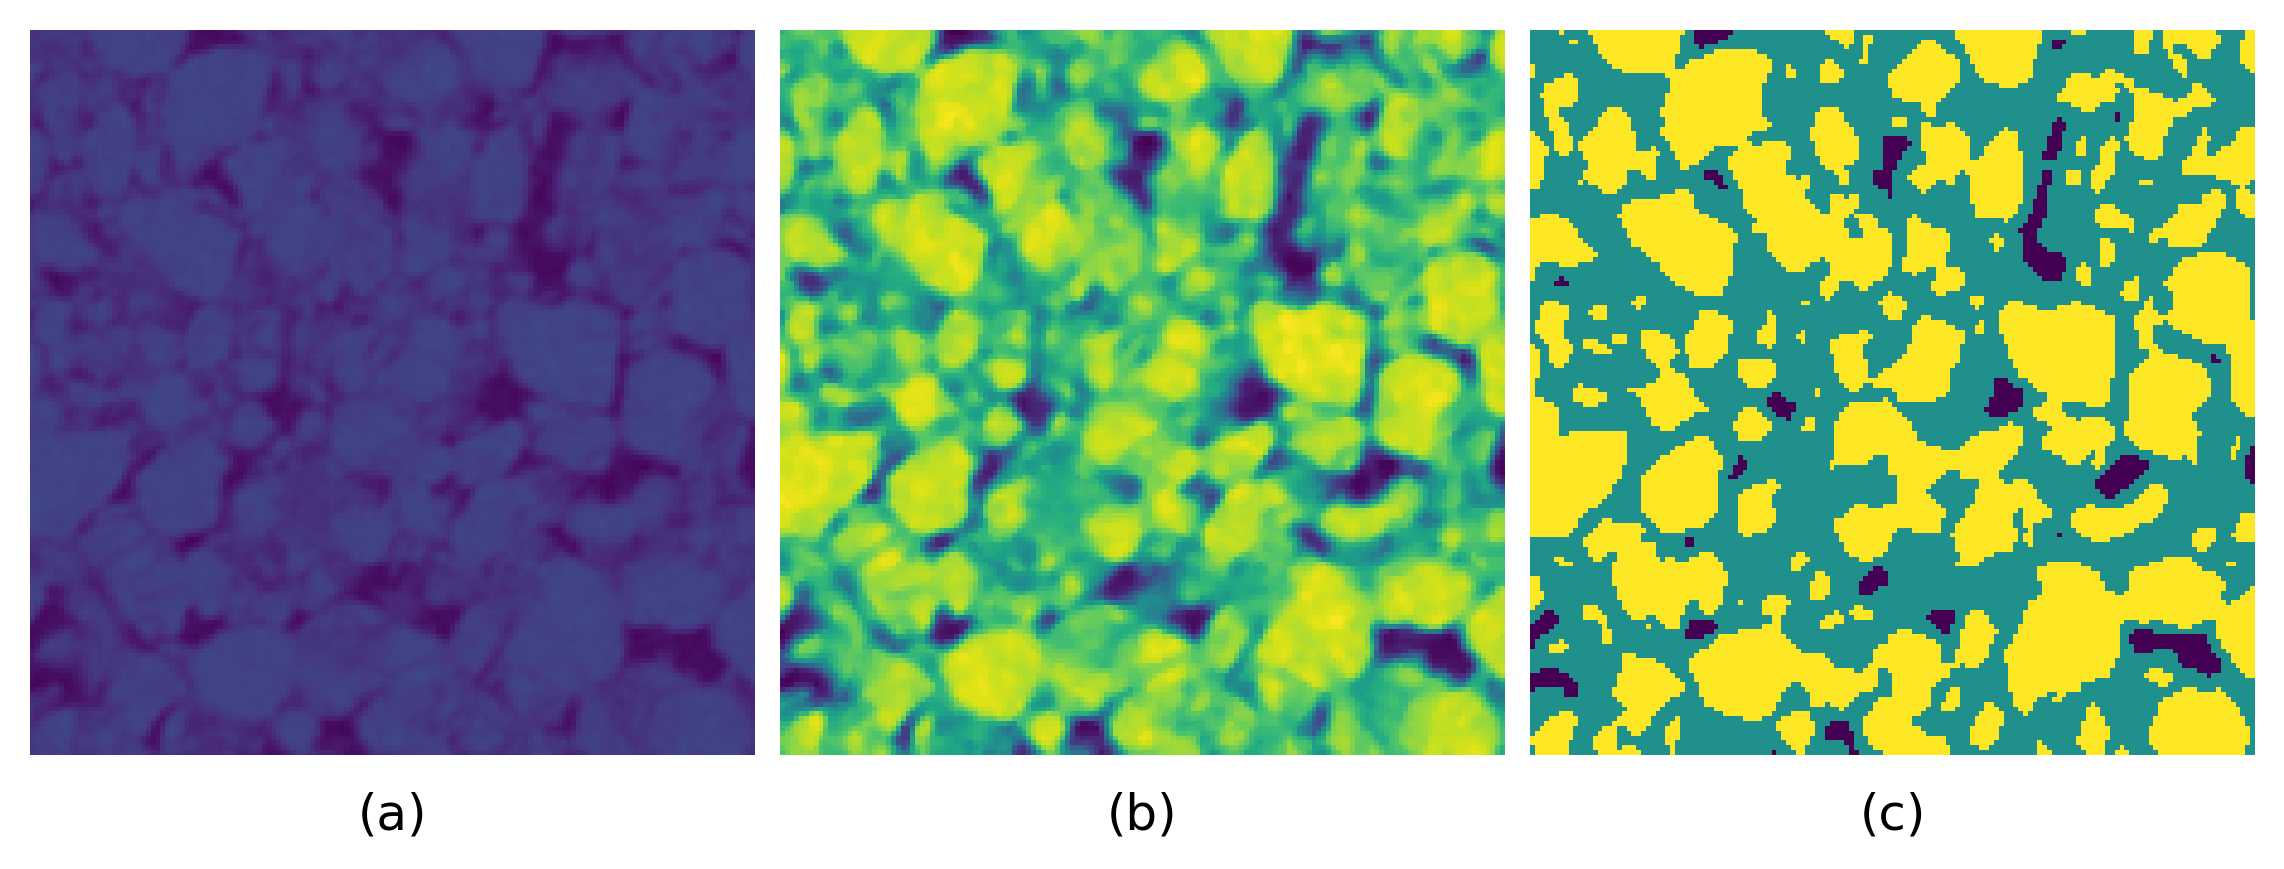
\includegraphics[width=0.75\textwidth]{figures/06/02-slice-525-semantic.png}
    \caption{
        \small\setstretch{1}
        (a) Low contrast image slice from raw CT scan.
        (b) Image slice after intensity is rescaled.
        (c) Semantic segmentation following thresholding of rescaled image
        using the minima of the smoothed histogram
        (\ref{fig/06/thresh}). The purple regions represent the
        void class, the blue regions represent the binder class, and the
        yellow regions represent the sand grain class.
    }
    \label{fig/06/semantic}
\end{figure}

\subsection{Instance Segmentation}
% -------------------------------------------------------------------------
\textit{Segmentflow}
uses a watershed algorithm in 3D to perform instance
segmentations. First a distance map is calculated by applying an EDT algorithm
implemented in \textit{scikit-image} to a binary image.
In the case of this demonstration of the F50 sand sample, a distance map
is created using the binary image corresponding to the sand grain class.
Local maxima are calculated to determine the markers which will
seed the watershed algorithm.
The 2D metaphor of watershed flooding does not
extend well to 3D, but the marker points act as the starting locations from
which the segmented regions will ``grow'' outwards.
Not all local maxima from the distance map are used as markers. Only the
maxima separated by a minimum distance are used.
The final segmentation depends greatly on
this minimum peak distance value as the number of markers is equal to the
number of labeled features, or segmented particles, in the resulting
segmentation.
If this value is too large, the results will be under-segmented as
fewer markers than sufficient are passed to the watershed algorithm,
excluding maxima that are closer together than this minimum distance.
This would create segmented particles larger than the true sand grains.
If the value is too large, the opposite will be true: too many maxima are
identified and passed to the watershed algorithm as seeds. With more markers
than necessary, the results will be over-segmented as separate markers
identified in the same feature will split that feature into multiple segmented
regions. This would produce segmented particles smaller than the true sand
grains.
Segmentations were performed at a range of minimum peak distances and
the resulting particles were analyzed to determine which minimum peak
distance value yielded particle sizes closest to typical F50 sand.

\subsubsection{Surface Mesh Creation}
% -------------------------------------------------------------------------
Depending on simulation type, a voxel representation of the segmented
particles may be an adequate format for the geometry. However,
some simulations require geometries be represented as a surface mesh
rather than voxels. Segmentflow can output triangular surface meshes saved
as STL files for each feature segmented.
There are currently two voxel preprocessing methods available in
\textit{Segmentflow} to
simplify geometries before any surface meshes are created: voxel smoothing
and morphologic erosion. For each method, the voxels of each segmented
feature are first isolated in a new 3D array. In voxel smoothing, a median
filter is applied to the voxels such that each voxel is replaced by the
median value (foreground or background) of the surrounding voxels (3 x 3 x 3
cube).
In morphologic erosion, the outer layer of voxels is removed, as if
peeling an onion. This is performed using an algorithm implemented in
\textit{scikit-image}. The algorithm can be applied multiple times
(peeling multiple onion skins) to further reduce the overall size of a
feature. This can be useful to ensure voxels of separately segmented
features are not in contact.
After these steps, surface meshes are created
for the segmented features using a marching cubes algorithm. This algorithm
takes the voxels at the surface of the 3D feature and generates
a surface consisting of vertices and triangles connecting the vertices
\cite{Lorensen1987, Lewiner2003}.
Each triangle has one of 26
possible normals based on the position of the other surface voxels in the
immediate vicinity: six possibilities for the Cartesian vectors when
neighbors of a voxel form a flat surface, 12 vectors when the voxels form
an edge, and eight vectors when voxels form a corner.
The \textit{scikit-image} implementation of the algorithm allows a voxel step
size to specified
to control the granularity of the voxels used to create the surface
mesh. If a step size of 1 is used, each voxel is analyzed to create the
surface mesh, whereas step sizes larger than 1 produce coarser mesh
results, compromising finer-scale details of the volume. Resulting surface
meshes can be saved as STL files.

\subsubsection{Surface Mesh Postprocessing}
% -------------------------------------------------------------------------
The surface meshes output from the marching cubes algorithm are blocky due
to the limited number of surface normals output from the data. This is an
artifact of the voxel nature of the data passed into the marching cubes
algorithm and is therefore not truly representative of real-world
geometries. \textit{Segmentflow} has two mesh postprocessing methods to further
process the 3D data: smoothing and mesh simplification.
Smoothing the blocky surface meshes
output by the marching cubes is achieved through Laplacian smoothing,
which interpolates normals vectors for the faces of a mesh. These meshes
may still have a large number of surface elements however because the
smoothing operation does not change the number of triangles. To reduce the
number of triangles, simplification can be performed through quadric
decimation \cite{Garland1997}. \textit{Segmentflow} implements the mesh
simplification by accepting a target number of triangles for the final
mesh and a scale factor that allows the number of triangles to be reduced
iteratively. Often smaller simplification factors yield better results
because more of a surface's shape is able to be retained between smaller
simplifications. Tuning the size of output surface meshes is an important
feature of \textit{Segmentflow} because the complexity of the meshes will
in part determine the scale of a simulation using the geometries.


% 6.3 Results
\subsection{Results}
Two separate methods were used to calculate the size distribution of
segmented particles resulting from different segmentations on the
same F50 sand and Kel-F CT scan.
Segmented particles were analyzed for watershed segmentations seeded with
markers determined with minimum peak distance values ranging from 4 to 8.
These values correlate to physical distances from 55.36 to 110.72 µm.
Each method determined whether or not a particle would be retained in a
separate way.
The first method
used spheres of equivalent volume for each segmented particle. The second
method used the aspect ratio of the bounding box of each particle.
To determine which minimum peak distance resulted in the most accurate size
distribution, each segmentation is compared with the
standard size distribution of F50 sand (\ref{fig/06/f50}).

\begin{figure}[ht]
    \centering
    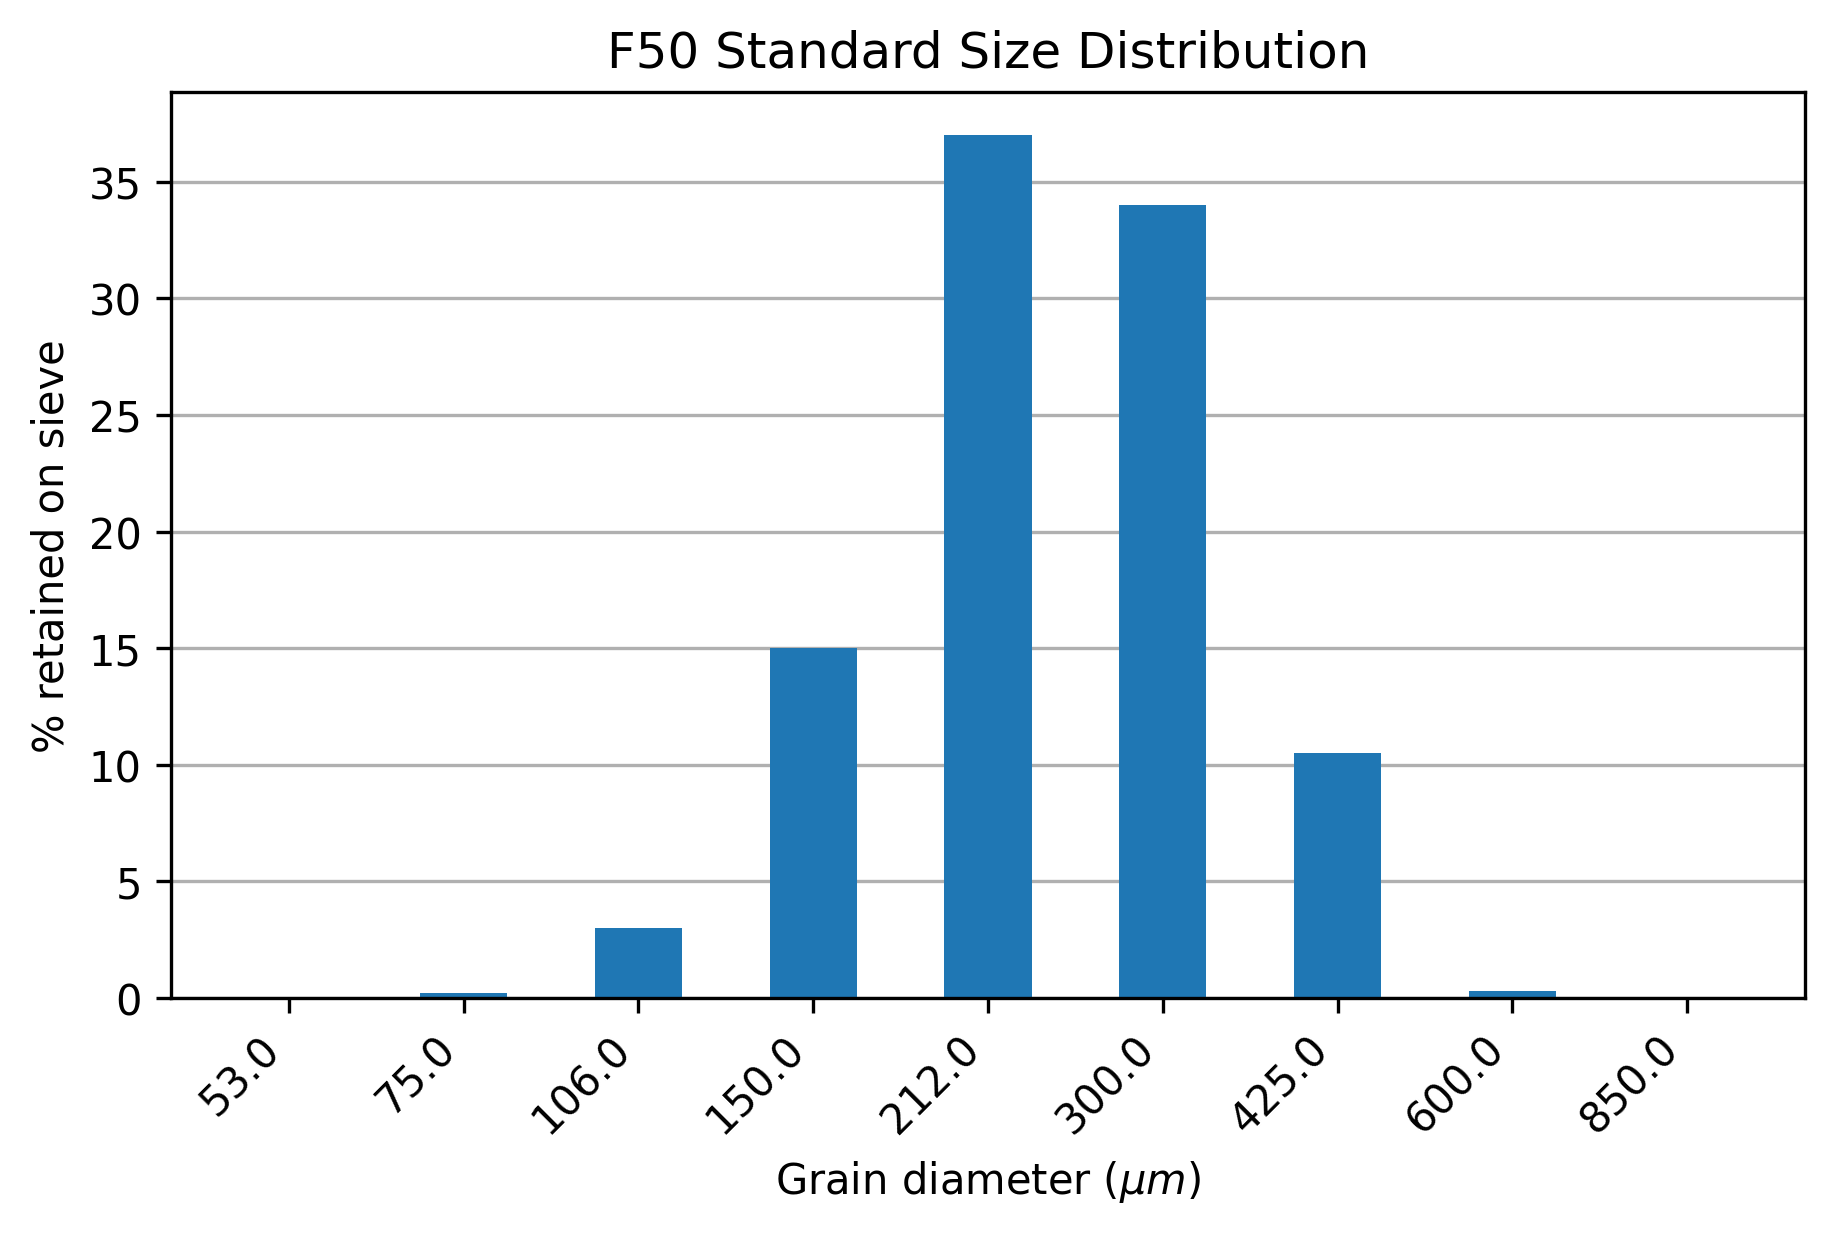
\includegraphics[width=0.75\textwidth]{figures/06/03-f50-size.png}
    \caption{
        \small\setstretch{1}
        Expected result from passing F50 sand through a series of sieves,
        expressed in percent of total grains retained at each step. Sieve
        size is given in microns.
    }
    \label{fig/06/f50}
\end{figure}

\subsubsection{Sphere of Equivalent Volume to Determine Size}
% -------------------------------------------------------------------------
The first method method for calculating segmented particle size distribution
took the volume of each particle,
calculated the diameter of the sphere with an equivalent volume, and used this
diameter to bin the particles between sieve mesh sizes
(\ref{fig/06/sphere}). The error between each
of the five segmentations was calculated as the cumulative difference between
the equivalent sphere distribution and the typical F50 distribution. These
errors are summarized for each segmentation in Table \ref{tab/06/error}.
The segmented particles seeded with a 6 pixel minimum peak distance has the
lowest error with a cumulative difference of 25.08\%. Particles seeded with
a 4 pixel minimum peak distance had the largest error at 79.29\%.

\begin{figure}[ht]
    \centering
    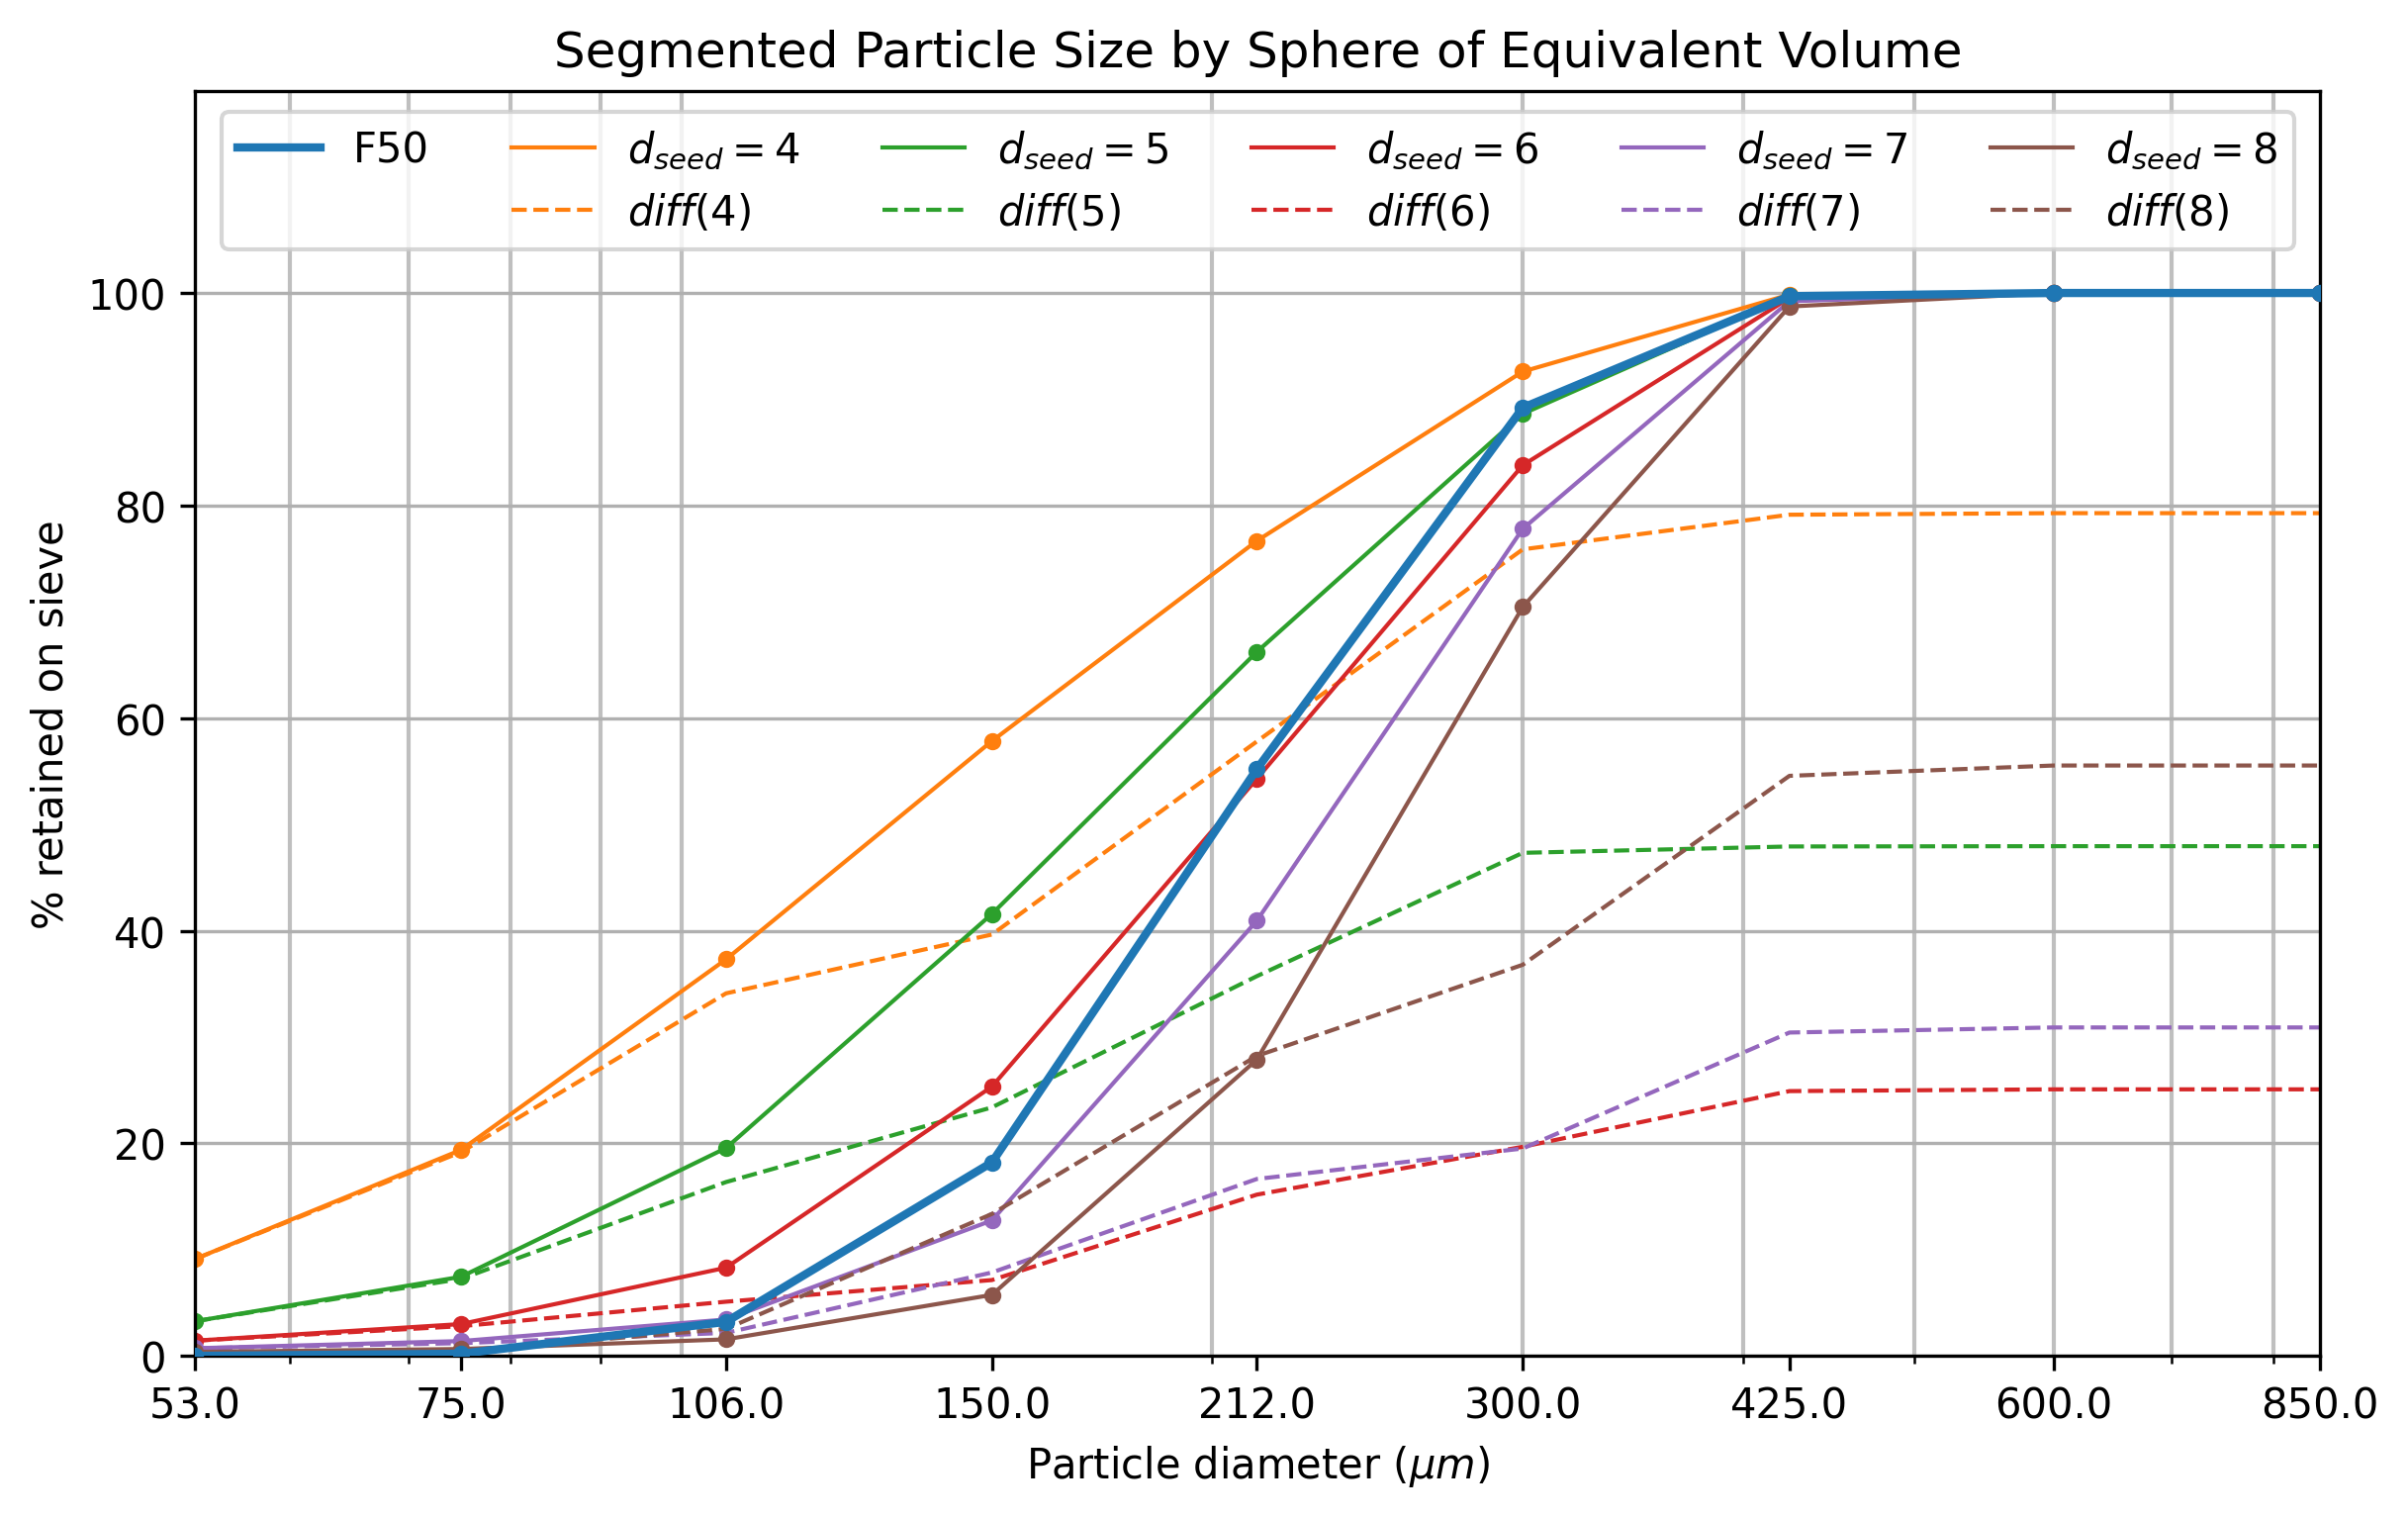
\includegraphics[width=0.75\textwidth]{figures/06/04-size-by-sphere.png}
    \caption{
        \small\setstretch{1}
        Size distribution of segmented particles binned
        according to the sphere of equivalent volume of each particle.
        Solid lines represent the cumulative distribution of particles at
        increasing sieve sizes. The blue solid line represents the typical
        values for F50 sand and the other solid lines represent the values
        determined from the particles obtained by segmenting the CT scan
        with a watershed algorithm seeded with different values for the
        minimum peak distance ($d_{seed}$). Dashed lines of corresponding
        color represent the error between the segmentation and typical values.
    }
    \label{fig/06/sphere}
\end{figure}

\subsubsection{Aspect Ratio of Bounding Box to Determine Size}
% -------------------------------------------------------------------------
The second method for calculating segmented particle size distribution
found the aspect ratio of the bounding box of each segmented particle and
used the maximum length of the minimum cross sectional area to bin the
particles (\ref{fig/06/aspect}). Just like with the equivalent sphere
method, the error between each
of the five segmentations was calculated as the cumulative difference between
the equivalent sphere distribution and the typical F50 distribution.
These errors are also summarized for each segmentation in Table \ref{tab/06/error}.
With this method of assessing the segmentations, the
particles segmented with a 5 pixel minimum peak distance have the lowest
error with a cumulative difference of 45.31\%. Particles seeded with an
8 pixel minimum peak distance had the largest error at nearly 95.59\%.

\begin{figure}[ht]
    \centering
    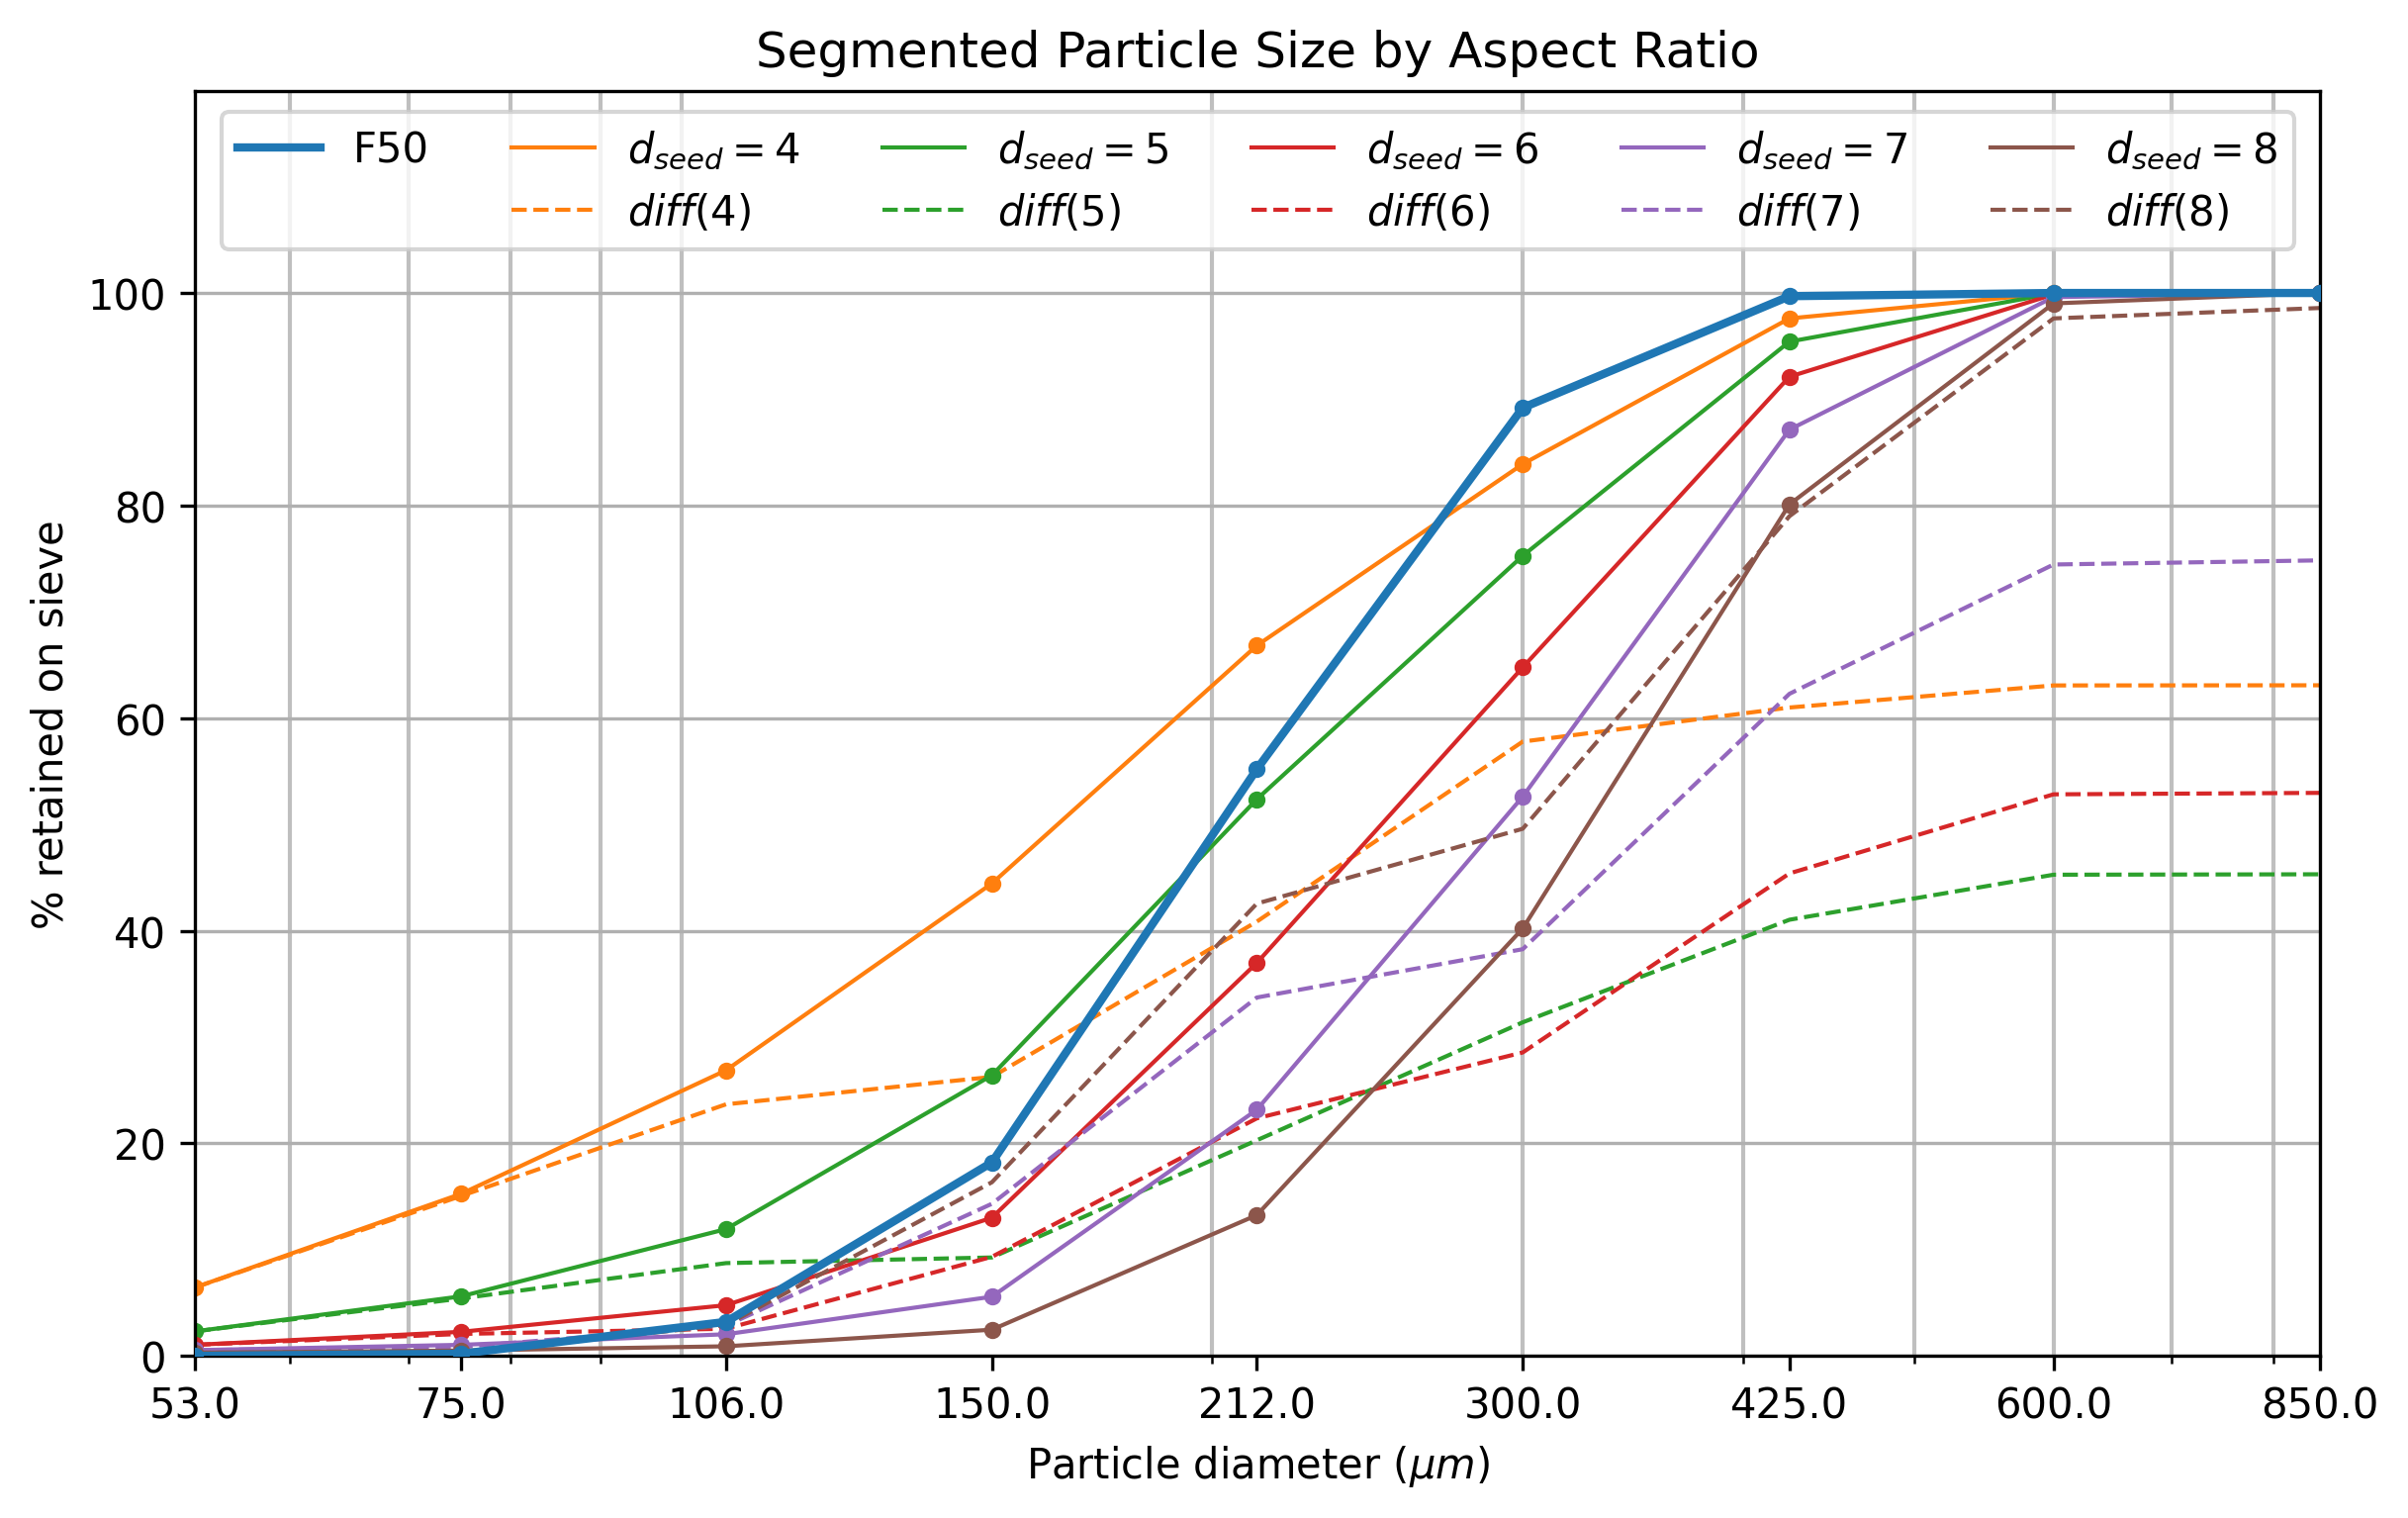
\includegraphics[width=0.75\textwidth]{figures/06/05-size-by-aspect.png}
    \caption{
        \small\setstretch{1}
        Size distribution of segmented particles binned
        according to the bounding box aspect ratio of each particle.
        Solid lines represent the cumulative distribution of particles at
        increasing sieve sizes. The blue solid line represents the typical
        values for F50 sand and the other solid lines represent the values
        determined from the particles obtained by segmenting the CT scan
        with a watershed algorithm seeded with different values for the
        minimum peak distance ($d_{seed}$). Dashed lines of corresponding
        color represent the error between the segmentation and typical values.
    }
    \label{fig/06/aspect}
\end{figure}

The sum of absolute errors for each segmentation are summarized in Table
\ref{tab/06/error}, combining
each method of determining the particle size, as well as the total error
which is the sum of the error from both methods. Based on these errors, the
watershed segmentation seeded with markers determined by a 6 pixel minimum peak
distance yields the results that most closely align with the typical F50 sand
size distribution.

\begin{table}[ht]
    \centering
    \caption{Segmented Particle Errors Relative to Typical F50 Sand}
    \label{tab/06/error}
    \renewcommand{\arraystretch}{1.5}% Spread rows out...
    \begin{tabular}{|>{\centering\bfseries}m{1in} >{\centering}m{0.75in} >{\centering}m{0.75in} >{\centering}m{0.75in} >{\centering}m{0.75in} >{\centering\arraybackslash}m{0.75in}|}
        \hline % \toprule
        Error             & \textbf{d\textsubscript{seed} = 4} & \textbf{d\textsubscript{seed} = 5} & \textbf{d\textsubscript{seed} = 6} & \textbf{d\textsubscript{seed} = 7} & \textbf{d\textsubscript{seed} = 8} \\
        \hline % \midrule
        Equivalent Sphere &  79.29 & 47.95 & 25.08 &  30.90 &  55.54 \\
        Aspect Ratio      &  63.09 & 45.31 & 52.97 &  74.84 &  95.59 \\
        Total             & 142.38 & 93.26 & 78.05 & 105.74 & 154.13 \\
        \hline % \bottomrule
    \end{tabular}
\end{table}

Using the optimal parameter as determined by measuring the size distributions,
this segmentation is used to generate surface meshes for the entire sample.

\begin{figure}[ht]
    \centering
    \includegraphics[width=0.9\textwidth]{figures/06/07-full-41553_particles.png}
    \caption{
        \small\setstretch{1}
        Surface meshes of all 41,553 particles segmented from the F50 sand
        sample loaded from three different views:
        (a) the top, (b) a high angle, and (c) the side.
    }
    \label{fig/06/full}
\end{figure}


% 6.4 Discussion
\subsection{Discussion}
% Hard to assess 3d seg from 2d image
% Compare differences at each number
A visual example of the findings from the size distribution
assessment is provided for the different segmentations of the
Kel-F - F50 sand system. A comparison is made between an image sliced from
the rescaled CT scan (\ref{fig/06/seg}.a) and the slice at the
corresponding location in each of the three segmentations determined to have
the lowest total accumulated error in size distribution. These segmentations
were seeded by markers selected with 5, 6, and 7 pixel minimum peak
distances and are hereafter referred to as
Segmentation B (\ref{fig/06/seg}.b), Segmentation C
(\ref{fig/06/seg}.c), and Segmentation D (\ref{fig/06/seg}.d),
respectively. Labeled sand grains of interest (\ref{fig/06/seg}.a) are
compared to corresponding segmented particles in each of these segmentations.

Across these segmentations, there is a trend of particles that are more
segmented in Segmentation B and become less segmented in Segmentation C and
Segmentation D.
There are not many over-segmented particles visible in this slice of the
volume, but the evidence over-segmentation can be seen in the segmented
representations of sand grain 3. In Segmentation B and Segmentation C this
sand grain is over-segmented as two particles. In Segmentation D, these two
regions are segmented as a single particle, but it is unclear from this
slice whether or not the sand grain to the lest is also merged into the
particle. Other sand grains are represented distinctly in Segmentation B
and Segmentation C but are erroneously under-segmented in Segmentation
D as is the case with sand grain 1 and sand grain 2 as well as sand grain 11
and sand grain X.
There are a few cases of sand grains segmented distinctly in Segmentation B
that are under-segmented in Segmentation C and Segmentation D. This occurs with
the pair of sand grains 8 and 9 as well as the group of particles 13, 14,
and 15.
Some particles are under-segmented in all three of the segmentations. This is
true of sand grains 5 and 6, which appear as a single particle in each
segmentation.
There are also certain cases in which sand grains that segmented distinctly in
Segmentation B appear to be un-segmented from surrounding binder material as
is the case with sand grains 4 and 12.
and what appears to be some of the surrounding binder material.
The final class of particles that appear here are particles in Segmentation B,
but are too small and close to other markers to appear in Segmentation C and
Segmentation D due to the minimum distance of the markers chosen to seed
these segmentations. This can be seen with sand grain 7.

All these examples show more under-segmented particles in Segmentation D
than in Segmentation B and Segmentation C, though Segmentation
B does have some under-segmented particles that appear to be properly
segmented in Segmentation B. Regardless, Segmentation B and Segmentation C
were both shown to minimize the
lowest total accumulated error in the two size distribution analyses in part
because the error was spread across the mean size of typically distributed
particles, with some smaller particles as well as some larger particles.
The other segmentations which resulted in higher total accumulated error
mainly had particles that were either majority smaller or majority larger
than the mean of the typical distribution.
The fact that Segmentation C had the lowest total accumulated error suggests
that the number of under-segmented particles balances out the over-segmented
particles that are also shown to be present.

% 3        over  over  well
% 1-2      well  well  under
% 4        well  well  under
% 12       well  under under
% 11       well  under under
% 8-9      well  under under
% 13-14-15 well  under under
% 5-6      under under under
% 7        well  xx    xx
% 10       well  well  well

\begin{figure}[ht]
    \centering
    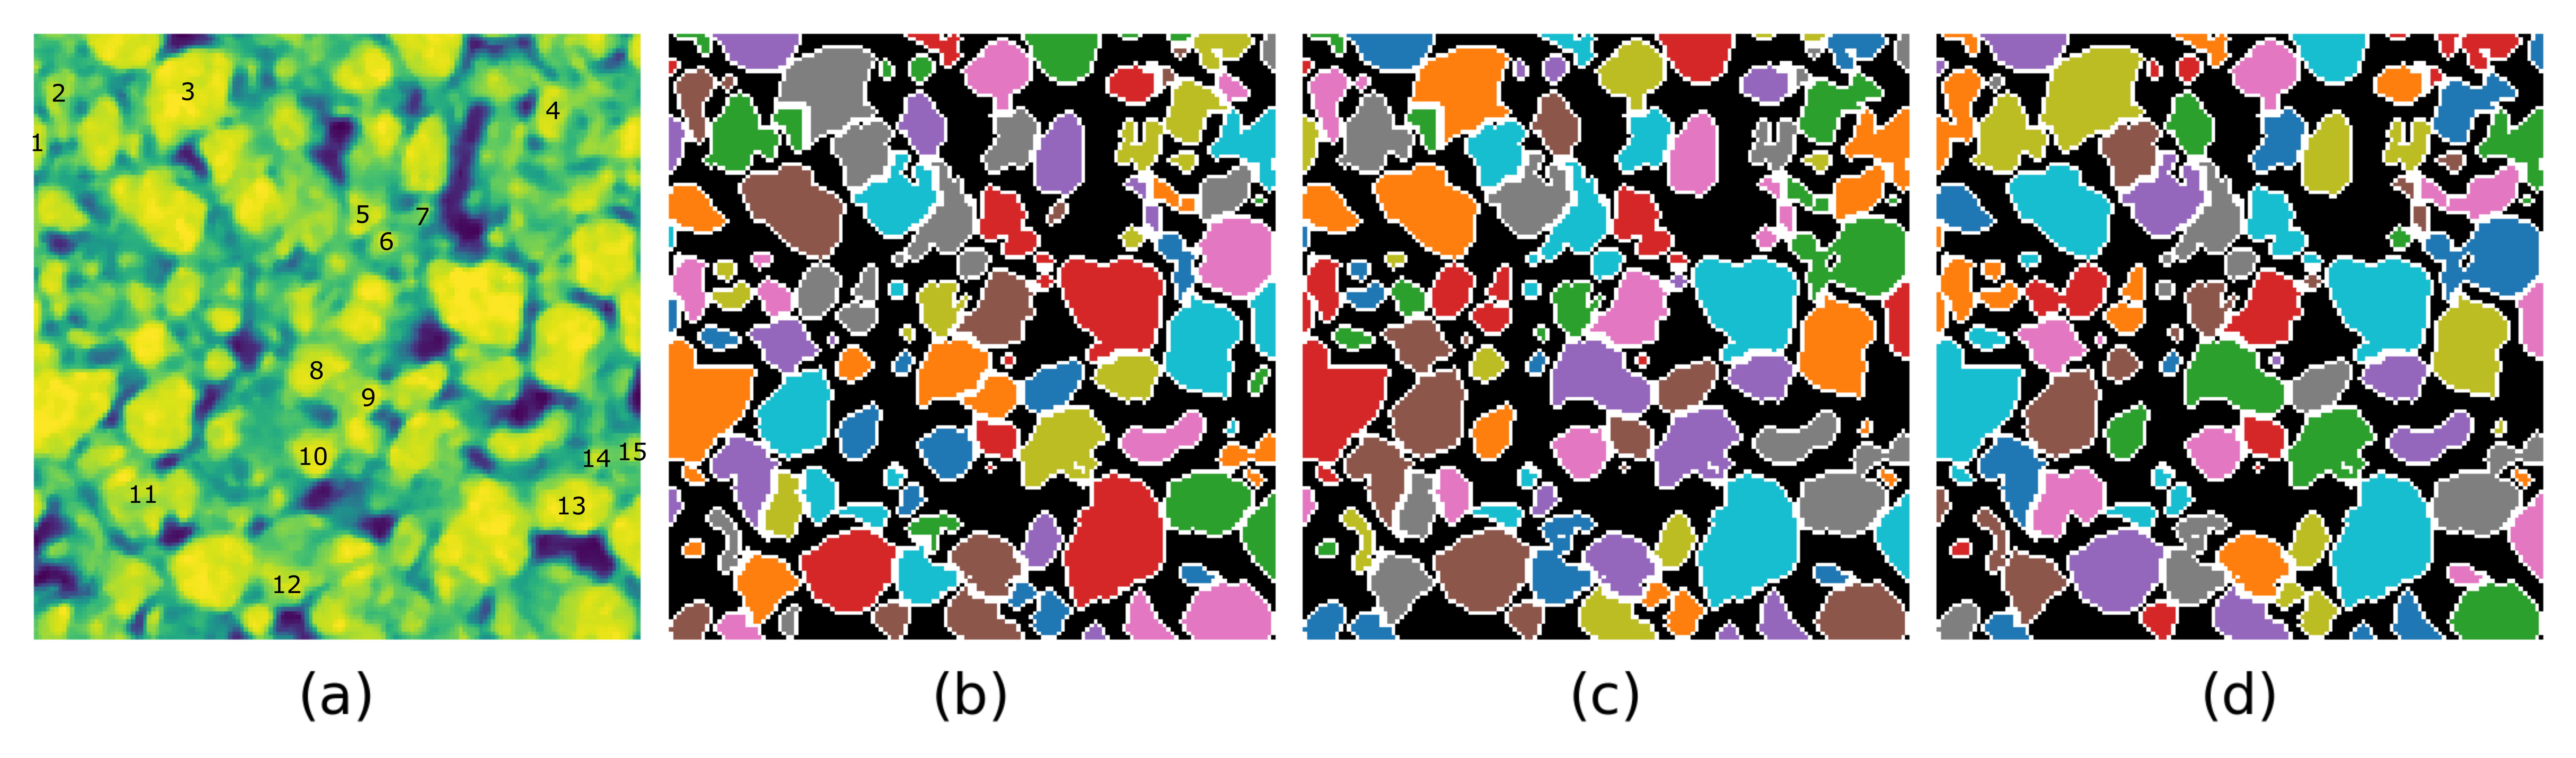
\includegraphics[width=0.9\textwidth]{figures/06/08-slice_525-full_seg-5-6-7.png}
    \caption{
        \small\setstretch{1}
        (a) A slice of the rescaled intensity CT scan image with particles of
        interest labeled to allow for ease of comparison and discussion
        between the three segmentations.
        (b) Corresponding slice of Segmentation B, as seeded by markers
        selected with a 5 pixel minimum peak distance, with the second lowest
        total accumulated error in particle size.
        (c) Corresponding slice of Segmentation C, as seeded by markers
        selected with a 6 pixel minimum peak distance, with the lowest
        total accumulated error in particle size.
        (d) Corresponding slice of Segmentation D, as seeded by markers
        selected with a 7 pixel minimum peak distance, with the third lowest
        total accumulated error in particle size.
    }
    \label{fig/06/seg}
\end{figure}

It is interesting that the watershed segmentation that performed the best was
seeded with markers determined with a 6 pixel minimum peak distance. This
correlates to a physical distance of 83.04 µm between markers,
which is between the second and
third smallest mesh sizes used to assess the particle sizes.
The 4 pixel minimum peak distance, which corresponds most closely to the
smallest mesh size (53 µm) at a physical distance of 55.36 µm, did not
produce results that aligned well with the typical size distribution, with
a total error among the highest of the tested segmentations. At a first glance,
this is unexpected, as one might expect the minimum space between markers to
be small enough to allow all the smallest particles to be segmented. However,
this result shows that it is actually more important to choose a larger
minimum peak distance to achieve a size distribution that is more
representative of reality. As can be seen in the left-shifted cumulative size
distributions of the 4 pixel minimum peak distance segmentation, the majority
of particles are smaller than typical F50 particles.
This means that generating markers based on a
distance that is closer to the size of the smallest particles results in
particles are over-segmented.
In contrast, the best fitting 5 and 6 pixel minimum peak distance segmentations
are distributed among each side of the typical F50 distribution, suggesting
a balance of over- and under-segmentation.

To demonstrate the mesh postprocessing capabilities of \textit{Segmentflow},
the surface mesh generated from the segmented particle corresponding to sand
grain 10 (\ref{fig/06/seg}.a) is shown independently and compared with
the meshes resulting varying amounts of postprocessing. The surface mesh
as-computed by the marching cubes algorithm is made up of 1524 triangles
(\ref{fig/06/postprocess}.a). After Laplacian smoothing, the mesh
retains the same number of triangles, but the result appears less blocky
(\ref{fig/06/postprocess}.b). The mesh is also shown after
simplification past 200 triangles, resulting in mesh made up of 190 triangles
(\ref{fig/06/postprocess}.c). The final mesh shows extreme
simplification past 20 triangles to a resulting mesh of only 10 triangles
(\ref{fig/06/postprocess}.d). This ability to tune the complexity of
the surfaces of each segmented particle is referred to as the
``exascale knob'' as it allows the user to determine the complexity of the
simulation which will use the resulting geometry.

\begin{figure}[ht]
    \centering
    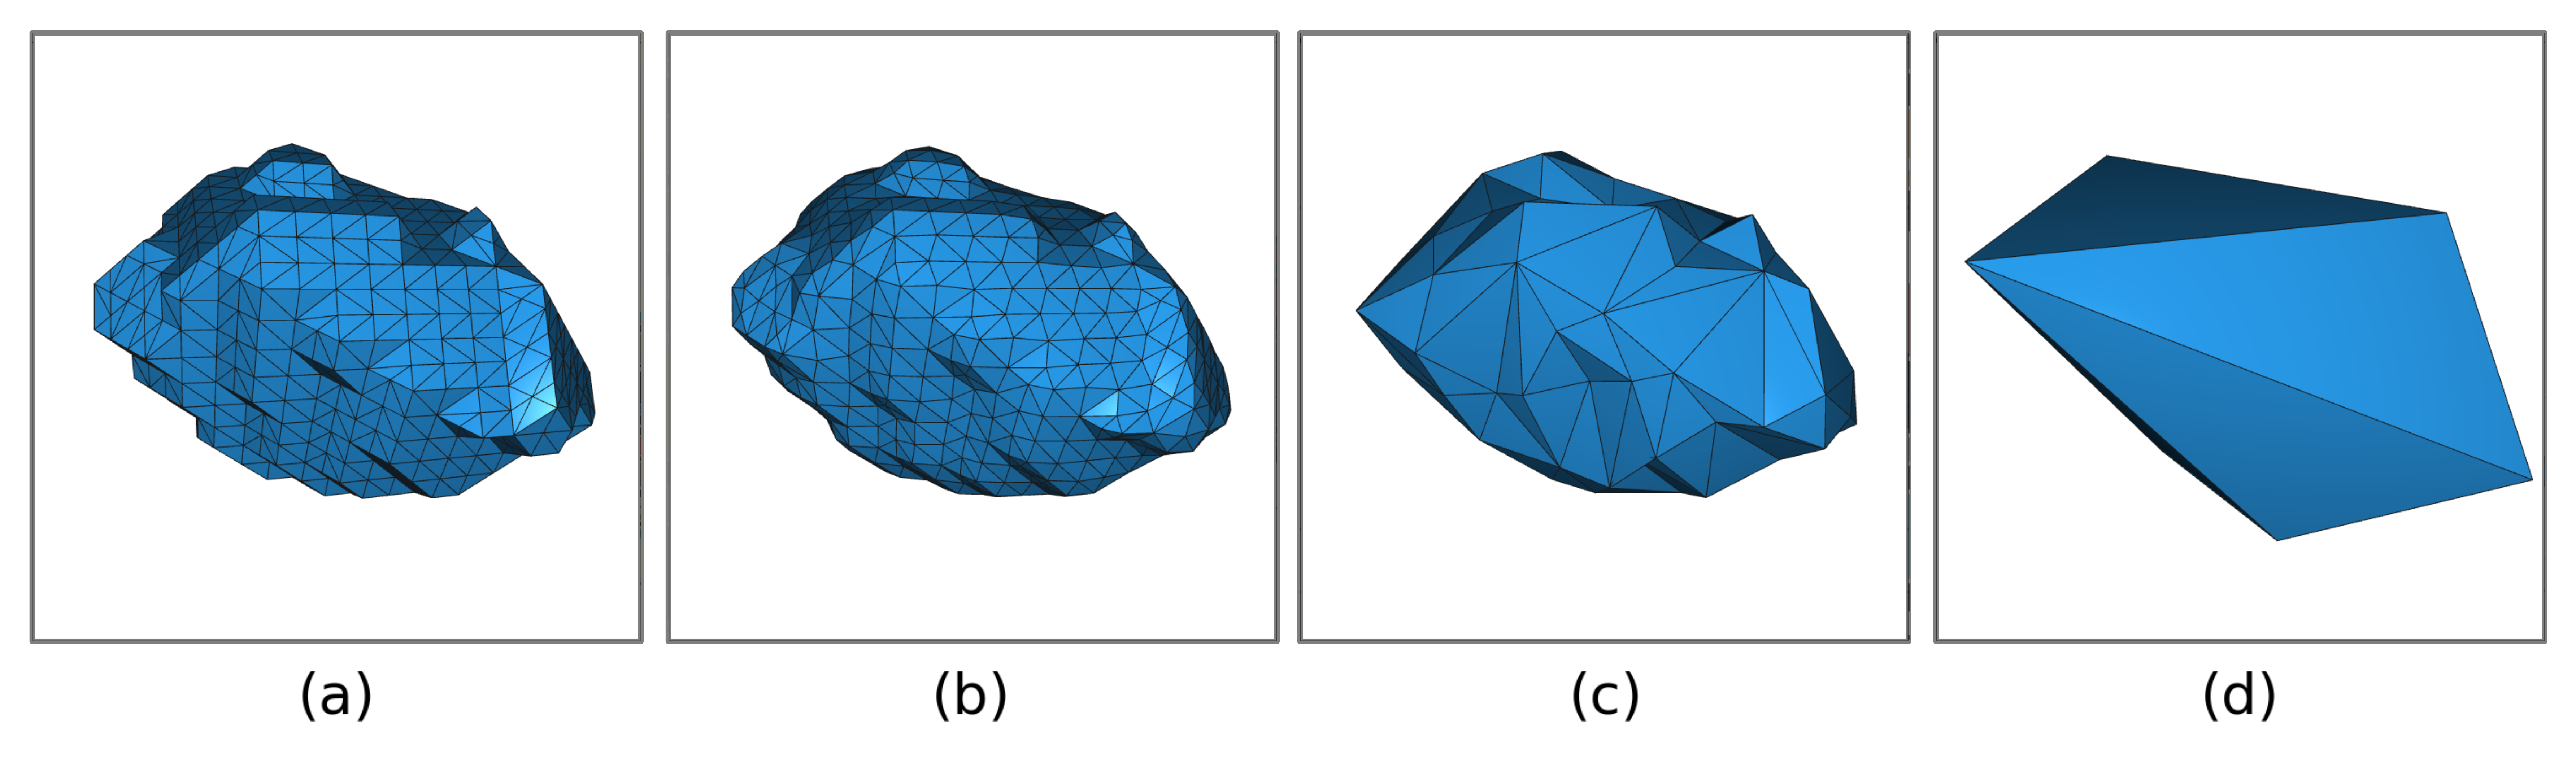
\includegraphics[width=0.9\textwidth]{figures/06/06-26259-mesh-tris-1524-190-10.png}
    \caption{
        \small\setstretch{1}
        (a) Surface mesh produced from a segmented particle. Mesh originally
        has 1524 triangles across its surface.
        (b) Smoothing applied to surface mesh as part of the mesh
        postprocessing capabilities of \textit{Segmentflow}.
        (c) Mesh simplified beyond 200 triangles.
        (d) Mesh simplified beyond 20 triangles.
    }
    \label{fig/06/postprocess}
\end{figure}


% 6.6 Conclusions
\subsection{Conclusions}
This work presents \textit{Segmentflow}, a segmentation workflow tool
that can be used to generate geometries for use in physics simulations.
A workflow is demonstrated that takes a CT scan of a mock high explosives
system consisting of F50 sand grains coated in a polymeric binder.
The CT scan was subject to a preprocessing procedure to increase the
contrast of the image, at which point it was semantically segmented
into regions labeled as one of three classes: void, binder, or sand grain.
The regions corresponding to the sand grain class were subject to an
instance segmentation procedure with the goal of segmenting and labeling
voxels identified as individual sand grains. These segmented particles are
dependent on the markers used to seed the segmentation algorithm.
A variety of markers were selected by specifying a range of minimum
distances separating the points. Each set of markers produced a different
segmentation. The segmented particles resulting from each separate
segmentation were analyzed to assess the segmentations.

Segmented particles resulting from five segmentations were analyzed.
The size distribution of the segmented particles
for each segmentation was compared with the typical F50 sand size
distribution to determine which segmentation yielded the most
accurate segmentation. Two methods were used to determine the size
distribution of the segmented particles from each segmentation. The first
method used the volume of each segmented particle and calculated the diameter
of the sphere of equivalent volume. This diameter was used to bin each
particle between the mesh sizes defined by the typical F50 distribution.
The second method used the aspect ratio of the bounding box of each particle
and used the maximum length of the minimum cross section of the box to bin
the particles. The sum of accumulated error was calculated for each method
and the total accumulated error, summing the error from each method,
was calculated for each of the five segmentations. The segmentation that
was seeded by markers with a 6 pixel (83.04 µm) minimum peak distance was
determined to have the lowest total accumulated error. A slice corresponding
to the same location of the sample volume was taken from each of the
three segmentations with lowest error and compared to provide a visual
example of the quality of the segmentations.

The segmented particles resulting from the segmentation with lowest error
was used to demonstrate the surface meshing capabilities of
\textit{Segmentflow}. The surface meshes were visualized together to show
the complete geometry of the sample. Postprocessing capabilities were also
demonstrated by comparing the unaltered surface mesh with smoothed and
simplified representations. The particle was shown to maintain its
general shape even when the number of triangles making up the surface
was reduced by more than two orders of magnitude. This shows an important
ability of \textit{Segmentflow} to control the complexity of geometries
and therefore the simulations for which these geometries will be used.



% -------------------------------------------------------------------------
%   Chapter 7
% -------------------------------------------------------------------------
\chapter{SUMMARY AND CONCLUSIONS} \label{ch/summary}
% Chapter 7: Summary and Conclusions
This chapter summarizes the each previous chapter.
Conclusions are also provided which address each of the research-driving
questions posed in Chapter \ref{ch/intro}.

\subsection{Summary}
% -------------------------------------------------------------------------
Following the introduction in Chapter \ref{ch/intro} and the literature
review presented in Chapter \ref{ch/lit-review}, many topics were
covered in Chapters \ref{ch/xray} through \ref{ch/sf}.
Chapter \ref{ch/xray}
presented a method for correlating x-ray intensity to sample composition
by comparing intensity profiles in a radiograph to an EDS line scans
measuring composition.
Chapter \ref{ch/melt} presented two automated procedures for identifying
and tracking the solidification of metallic samples following
laser melting. The results from each procedure were compared to manual
measurements to assess the success of the automation.
Chapter \ref{ch/seg} presented a new method for the segmentation of
irregular particles that cannot be accurately segmented
with usual methods described in literature. This method proposed an
extension to a typical segmentation method that produced results that
were calculated to more closely match a manual segmentation than a
typical segmentation on its own.
Chapter \ref{ch/sf} presented a Python package developed to establish
a workflow for creating 3D geometries from images to be used in physics
simulations. A segmentation workflow is demonstrated to generate surface
meshes from an XCT scan of the plastic explosive surrogate material
system F50 sand and Kel-F. Resulting segmented particles are analyzed
by comparison with a typical size distribution of F50 sand.

\subsection{Conclusions}
% -------------------------------------------------------------------------
The work presented in Chapters \ref{ch/xray} through \ref{ch/sf} each
address one of the research questions posed in Chapter \ref{ch/intro}.
Conclusions for the work presented in each chapter are presented below in
the context of the corresponding research question which drove the work.

\subsubsection{Relating X-Radiography to Composition}
% -------------------------------------------------------------------------
\noindent \textit{
    How can in-situ x-radiography be used in conjunction with
    other methods of analysis to infer composition of an Al-Ag alloy during
    solidification?
}

Chapter \ref{ch/xray} proposed a proof-of-concept, multimodal approach
to solidification analysis of an Al-Ag alloy system combining three
separate methods of investigation.
In-situ x-radiography measured changing grayscale intensities
through the sample volume during solidification,
EDS measured composition at the surface of the as-solidified
sample, and the calculation of a Scheil solidification model
which provided compositional information throughout a theoretical
solidification.
Aligning the final x-radiograph with the SEM image
showing the track of the track of the EDS scan allowed for an intensity
profile to be generated along the same solidified structure. Even though
the radiography captured the entire thickness of the sample and the
EDS measured only the surface, the two datasets showed similar trends
in multiple regions in the sample. These trends show that a mapping
from x-ray intensity to composition could be possible without performing
an explicit calibration experiment.
The Scheil solidification model calculated the composition of the solid
forming at different temperatures, simulating the solidification of an
alloy system matching that of the sample. The resulting data was plotted
as solid composition versus fraction solid. This data was fit to the
manually annotated radiographs to create a mapping from the image number
to solid composition. The as-measured data fits reasonably well at the
beginning of the solidification, though after about 75\% of the sample
solidified, the fraction solid as-measured was larger than the values
calculated from the Scheil model. A potential cause for this discrepancy
was that manually annotated solidifying structures, used to calculate
solid fraction, were not completely solidified through the entire
thickness of the sample as assumed.
While this work did not make direct correlations between these three
analysis methods, the comparisons provided more insight into the
solidification than either of the three methods would have provided on
its own.
With more experiments performed, the relationships between the different
methods could be identified to more confidently infer composition from
the in-situ x-radiography intensities.

\subsubsection{Procedural Analysis of Melt Pool Tracking}
% -------------------------------------------------------------------------
\noindent \textit{
    How successful is an image processing procedure at automating the
    identification, tracking, and velocity calculation of solid-liquid interfaces
    during in-situ solidification experiments?
}

Chapter \ref{ch/melt} explored the efficacy of automated procedures for
identifying, tracking, and calculating the velocity of metallic solidification
processes observed in situ. Two types of procedures were developed and tested:
the first for synchrotron x-radiography monitoring of AM
simulator experiments and the second for DTEM monitoring of thin film,
rapid solidification experiments.
The results from each procedure were compared to manual measurements. In the
AM simulator experiments, the automated procedure was reasonably successful
identifying the interfaces when compared to the manual measurements.
For two of the three experiments on which the procedure was applied, the
mean solidification velocity calculated from the detected interfaces
was drastically different than the manually measured velocities,
but the median values were similar. The average deviation from the manual
mean velocity was also higher for the detected data, but half the detected
data were within the average deviation for one of the experiments, and the
majority for the other experiment, which suggests that the error
in the detected measurements was mainly due to large outliers from
detected noise. In the third experiment, the mean detected velocity
was the same as the mean manual velocity, but the median velocities
differed. This suggests that the deviations were balanced above and below
the mean. Like the previous experiments, the average deviation from the
manual mean was still higher for the detected velocities than for the
manual measurements, but the majority of detected data was within the
average deviation from the manual mean, suggesting once again that the
majority of the error comes from the outliers in the data.

In the rapid solidification experiments, the outlined procedure is able
to accurately track the interface throughout the entire solidification
process according to comparisons with the manual measurements. The velocity
calculations were also in agreement with the manual calculations for the
majority of the experiments, with the exception of the end of the third
experiment where the melt pool much smaller and disappears before the last
frame of the experiment. One reason the rapid solidification procedure
performed better than the AM simulator procedure is because the melt pools
generally stayed large enough to not be confused with noise (besides the
end of the third experiment). The rapid solidification procedure also
incorporated an optimization step. If something similar was included for
the AM simulator experiment, the results might have been less sensitive
to noise.

Beyond comparisons to manual results, there are additional benefits
to the development of these automated procedures.
Automated procedures allow for more consistent results
than manual measurements. A procedure carried out by a computer will be
performed the same way on any given dataset, regardless of the experience or
biases of the user executing the method.
The process of developing automated procedures may also be beneficial to
the scientific process. When explicitly writing out a routine such that
it can be interpreted by a computer, researchers may more closely consider
their methods in a way uncovers previous unnoticed bias. Less justified
analysis steps may be left out when a routine is made more explicit.
Finally, automatic methods may encourage researchers to test changes in
analysis methods which could lead to more refined results.
One barrier to refining analysis methods is the effort and time required to
test changes to these methods. Especially when results are not guaranteed to
improve, high time and effort barriers may prevent these results from being
tested. This can lead to analysis methods that deliver "good enough" results
rather than analysis methods that are proven to be superior to other methods.
However, with automated procedures, more iterations of analysis methods can
be tested without the same time and effort commitment. This increases the
chance that improvements to the analysis method can be discovered to improve
results that otherwise may not have been tested.

Overall, the success of image processing procedures in identifying, tracking,
and calculating the velocity of solid-liquid interfaces was shown to be mixed
when the measure of success is the accuracy related to manually determined
values. The accuracy in the procedure which included an optimization
step (thin film rapid solidification experiments) outperformed the procedure
which did not include any optimization (AM simulator experiments). This
suggests that incorporating an optimization step should be considered in
development of similar procedures. Other benefits may include quantifying
consistency, bias reduction, and time/effort reduction for tuning results.

\subsubsection{Segmentation of Irregular and Tightly Clustered Particles}
% -------------------------------------------------------------------------
\noindent \textit{
    How can the segmentation of multi-sized, irregularly-shaped, and
    tightly-clustered particles be improved?
}

Chapter \ref{ch/seg} proposed a method for improving the segmentation
of irregularly distributed features (e.g., sand grains) that are not
accurately segmented using
methods found in literature. A common method in literature for segmenting
features of an image is the application of a watershed algorithm.
Watershed segmentation enables features
in contact with one another to be segmented as long as the size and shape of
the features are roughly uniform.
Even when the shapes are nonuniform, watershed segmentation can return
accurate segmentation results as long as the features are roughly the same
size. An adjustment to the routine can also be made that allows for
multi-sized features to be segmented from one another, solving either over-
or under-segmentation in these cases, as described in
the introduction of Chapter \ref{ch/seg}.
However, when features are not uniform in size or shape,
the typical watershed segmentation does not yield accurate results.
This inaccuracy is amplified when particles are clustered tightly
enough to be misrepresented as even more irregular particles.
The irregularity causes the resulting segmentation to contained a
combination of over- and under-segmentation, which cannot be adjusted by
methods in literature.

This chapter presented an extension to typical watershed segmentation by
including additional preprocessing steps which would intentionally generate
over-segmented results. These resulting regions where then subject to a novel
algorithm for merging regions based on edge strength between neighboring
regions. This proposed algorithm relied on a Delaunay triangulation that
identified neighboring regions across varying distances. These varying
distances allowed for multi-sized features to be considered.
The algorithm also relied on an assumption that neighboring regions
adequately segmented would see an increase in intensity in an edge-amplified
image. By assuming these spikes would not occur between two under-segmented
features, the lack of presence of these spikes was used as a merging
condition for neighboring regions.
This method was tested on a 2D image taken from a 3D XCT scan of
material system consisting of irregularly sized and shaped sand grains
tightly clustered with a polymer binder. The results of the merged region
segmentation were compared to a manual segmentation of the same image,
along with the results from a typical watershed segmentation.
The merged region segmentation achieved a fit of 89.02\%, a 6.93\%
improvement from the typical watershed segmentation.

\subsubsection{Generating Image-Based Modeling Geometries}
% -------------------------------------------------------------------------
\noindent \textit{
    How can a workflow be designed to extract 3D geometries from x-ray
    computed tomography data such that the geometry of a physical sample can be
    reproduced digitally for use as initial conditions in an image-based physics
    simulation?
}

Chapter \ref{ch/sf} presented \textit{Segmentflow}, a Python package
for building and/or executing segmentation workflows to extract
information from 3D datasets like XCT scans. The goal of these workflows
is to create physically informed geometries for use in image-based physics
simulations. \textit{Segmentflow} has tools for loading data and segmentation
parameters, preprocessing images to improve contrast and/or reduce noise,
performing semantic segmentation to classify scan data according to material
type/class, performing instance segmentation by watershed algorithm,
converting voxel data to surface meshes, and postprocessing surface meshes
to fit the needs of a particular simulation/user.

Functionality of \textit{Segmentflow} was presented by demonstrating a
segmentation workflow for generating simulation-ready surface meshes from
an XCT scan of a F50 sand and Kel-F binder system used to approximate the
mechanical properties of high explosives. The XCT data was
loaded with \textit{Segmentflow} and preprocessed to improve the contrast.
The sample was expected to have three classes of material represented
in the images: void, binder, and sand grain. Threshold values were calculated
to segment the volume into these three classes, and a binary image was
created to distinguish the sand grain class from the rest of the classes.
This binary representation was used to calculate a set of markers which will
each seed a watershed segmentation for a total of five separate
segmentations. The resulting
segmented particles from each of these segmentations were analyzed to
calculate a size distribution calculated in two ways: from the sphere
of equivalent volume and from the aspect ratio of the bounding box. The
segmentation that produced particles with the smallest total accumulated
error summed across both size distributions was assumed to be the most
accurate. These segmented particles were converted to surface meshes, and
all 41553 surface meshes were visualized together to show the extent of the
sample. One of the particle surface meshes was used to show an example of mesh
postprocessing. The example surface mesh, originally consisting of 1524
triangles, was visualized side by side with the same surface mesh after
a series of postprocessing steps. The first step shows the particle after
Laplacian smoothing. This retains the number of triangles, but results in
a surface mesh that appears less blocky. The next step shows the surface
mesh after simplifying past 200 triangles to a total of 190 triangles. The
final step shows the surface mesh reduced past 20 triangles
to a total of only 10 triangles. This series of postprocessing steps
shows how the surface mesh can be reduced drastically. This is an important
capability of \textit{Segmentflow} as it gives the user the power to create
simulation geometry that can have a range of complexity, depending on the
desired scale of the simulation.





% -------------------------------------------------------------------------
%   Chapter 8
% -------------------------------------------------------------------------
\chapter{RECOMMENDATIONS FOR FUTURE WORK} \label{ch/future}
% Chapter 7: Recommendations for Future Work
The work presented in this thesis answered questions that were sought at
the beginning of the project. In the process, however, more questions
were discovered. These discoveries provide opportunities
to compound the results presented in this thesis.
This chapter addresses these opportunities by providing 
recommendations for future work. 

\subsection{Optimization of AM Simulator Detection}
% -------------------------------------------------------------------------
In Chapter \ref{ch/melt}, two procedures were presented detect the
solid-liquid interface in a solidifying metal sample. The procedure
developed first was for AM simulator experiments and was designed to
detect semi-elliptical melt pools. The second procedure,
developed after the first, was designed to detect elliptical melt pools in
thin film, rapid solidification experiments.
The procedures were similar, but the AM simulator procedure detected the
bounding box of the semi-elliptical melt pools whereas the rapid
solidification experiment optimized the fit of an ellipse to the
elliptical melt pool. The rapid solidification procedure performed better
than the AM simulator procedure. The incorporation of fit optimization may
not have been the only reason for the improved performance, but
incorporating some kind of an optimization step into the AM simulator
would be a good place to start improving the procedure.

The optimization included in the rapid solidification procedure optimized
the fit of an ellipse to the melt pool. To bring optimization to the AM
simulator procedure, a shape could similarly be fit to the data. However,
the fit of the ellipse was optimized by minimizing a cost function that
incorporated the mismatch of the ellipse with a binary image
representation of the experiment. A cost function to be optimized to
improve the fit of the AM simulator could include many different
parameters besides fit mismatch. Other parameters could
include detected melt pool aspect ratio, difference in size
with the melt pool of the previous frame, difference in location of
with previous melt pool, location relative to the center of the image,
or location relative to the top of the sample.
Exploring the optimization using some of these parameters would make for
an interesting study that is likely to achieve promising results based
on the number of possibilities alone.

\subsection{Extension of Edge Strength Corrected Segmentation}
% -------------------------------------------------------------------------
In Chapter \ref{ch/seg}, a method was presented to correct the
segmentation of irregularly-shaped, multi-sized, and tightly-clustered
particles. The implementation of this algorithm was successful,
however the presented routine was only applied in two dimensions.
The image on which this routine was tested is itself from a
3D dataset. This displays the biggest opportunity to be
pursued following this work: adapting this routine to work with
3D data. The watershed segmentation and Delaunay
triangulation algorithms leveraged for this procedure can both function
in three dimensions, so the main focus would need to adapt the region
merging algorithm to 3D. A potential obstacle is the increase in the number
of neighbors for marker will in the adaption to 3D. This may require
optimization of the merging algorithm, depending on the size of the
datasets to which the procedure is applied.

Another path for continued study related to this method is further
development of the criteria defining detected edges.
The method as it stands has two conditions for detecting edges: a simple
threshold dependent on the maximum intensity of the edge-amplified
image and the location of any detected edges along the line connecting
two markers/regions. Perhaps by applying more thorough signal
processing techniques, a more robust criteria could be developed that
wouldn't require fine-tuning on an image-to-image basis that is likely
necessary with the current algorithms. A study on either or both of these
extensions to this method would be interesting and useful, especially for
the application of image-based simulations as discussed in Chapter \ref{ch/sf}.

\subsection{Additional Segmentation Functionality for Segmentflow}
% -------------------------------------------------------------------------
Chapter \ref{ch/sf} presented \textit{Segmentflow}, a Python package for
developing and/or executing segmentation workflows to create geometry
that could be used as initial conditions in a physics simulation.
\textit{Segmentflow} is a flexible software library that has been steadily
increasing the more it is used and the more diverse its user base has
become. There are many additional features that could be added, but some of
the most scientifically interesting include additional methods for
determining particle size distributions and the ability to merge
segmentation results. In Chapter \ref{ch/sf}, size distributions were
calculated for the segmented particles by binning particles by diameter as
determined by either assuming the particle was a sphere or using the maximum
bounds of a particle. The sphere method is obviously limited because
most particles are not actually spheres. For very blocky
particles, this may be an underestimate of size, but for most particles,
this will be a overestimate of size since the particles may have volume
distributed preferentially along one or two axes rather than all three
equally. The limitations of the bounding box method, which determines the
size based on the aspect ratio of the smallest box a particle could fit in
does a better job of not overestimating size based on volume distribution,
however, there are further limitations related to how a particle is oriented
within the box. The box is constrained to the axes of the voxels, so if an
oblong particle is oriented significantly askew to any of these axes, the
bounding box will be much larger than the particle. A better method for
approximating the size distribution of segmented particles would be to fit
a tightly fitting ellipsoid around each particle, however this is not
currently possible in \textit{Segmentflow}.

As discussed in Chapter \ref{ch/seg}, segmenting irregular
particles is difficult because if results are a mix of over- and
under-segmented, the segmentation cannot be improved in both directions,
which was the motivation for the Chapter \ref{ch/seg} in the first place.
Perhaps rather than trying to correct results from watershed segmentation,
methods of segmentation could be investigated. Many of the
incorrect results that can result from watershed segmentation have complex,
unnatural-looking forms. Rather than try to correct these forms after
segmentation, a new segmentation method might be able to avoid these forms
in the first place. One potential path for
this kind of a study would be to investigate a method to
incorporate minimization of surface energy into a segmentation algorithm.




% ><><><><><><><><><><><><><><><><><><><><><><><><><><><><><><><><><><><><><><><><
%                   BACK MATTER: Reference Cited
% ><><><><><><><><><><><><><><><><><><><><><><><><><><><><><><><><><><><><><><><><
\backmatter     % Leave this line here, it sets the formatting requirements for the back matter of the document

% >>>>>>>>> References Cited (required) <<<<<<<<<<
\urlstyle{rm}               % <-- Sets the URL font to be the same as the other text
\bibliography{supporting-files/thesis}

% Make sure the citations in you .bib file are correct. Especially double check that the resources type is correct. This will dictate how the items in the bibliography are formatted.

% Highly recommend using a citation/reference management tool to create your .bib file. This make your references machine readable in the click of a button. Attend a Libray workshop, visit the Library's website, or speak to a librarian about getting started with a citation management tool. This will make your life much easier. READ: MUCH EASIER! https://libguides.mines.edu/citing/software

% Look at http://bib-it.sourceforge.net/help/fieldsAndEntryTypes.php#phdthesis to find some information on the types of fields that exist. Also recommend using a reference manger. 


% >>>>>>>>> Appendices (if applicable) <<<<<<<<<<
\appendix{Copyright Permissions}

Proof of permission from the publisher and co-authors to reprint
the 2023 JOM article
``Integrating In Situ x-Ray Imaging, Energy Dispersive
Spectroscopy, and Calculated Phase Diagram Analysis
of Solute Segregation During Solidification of an Al-Ag Alloy''
\cite{Becker2021}
as Chapter \ref{ch/xray}.

\subsection{Permission from Publisher}
The following pages express permission from the publisher of JOM,
Springer Nature, to reprint the journal article in question as part of
this thesis.
\newpage
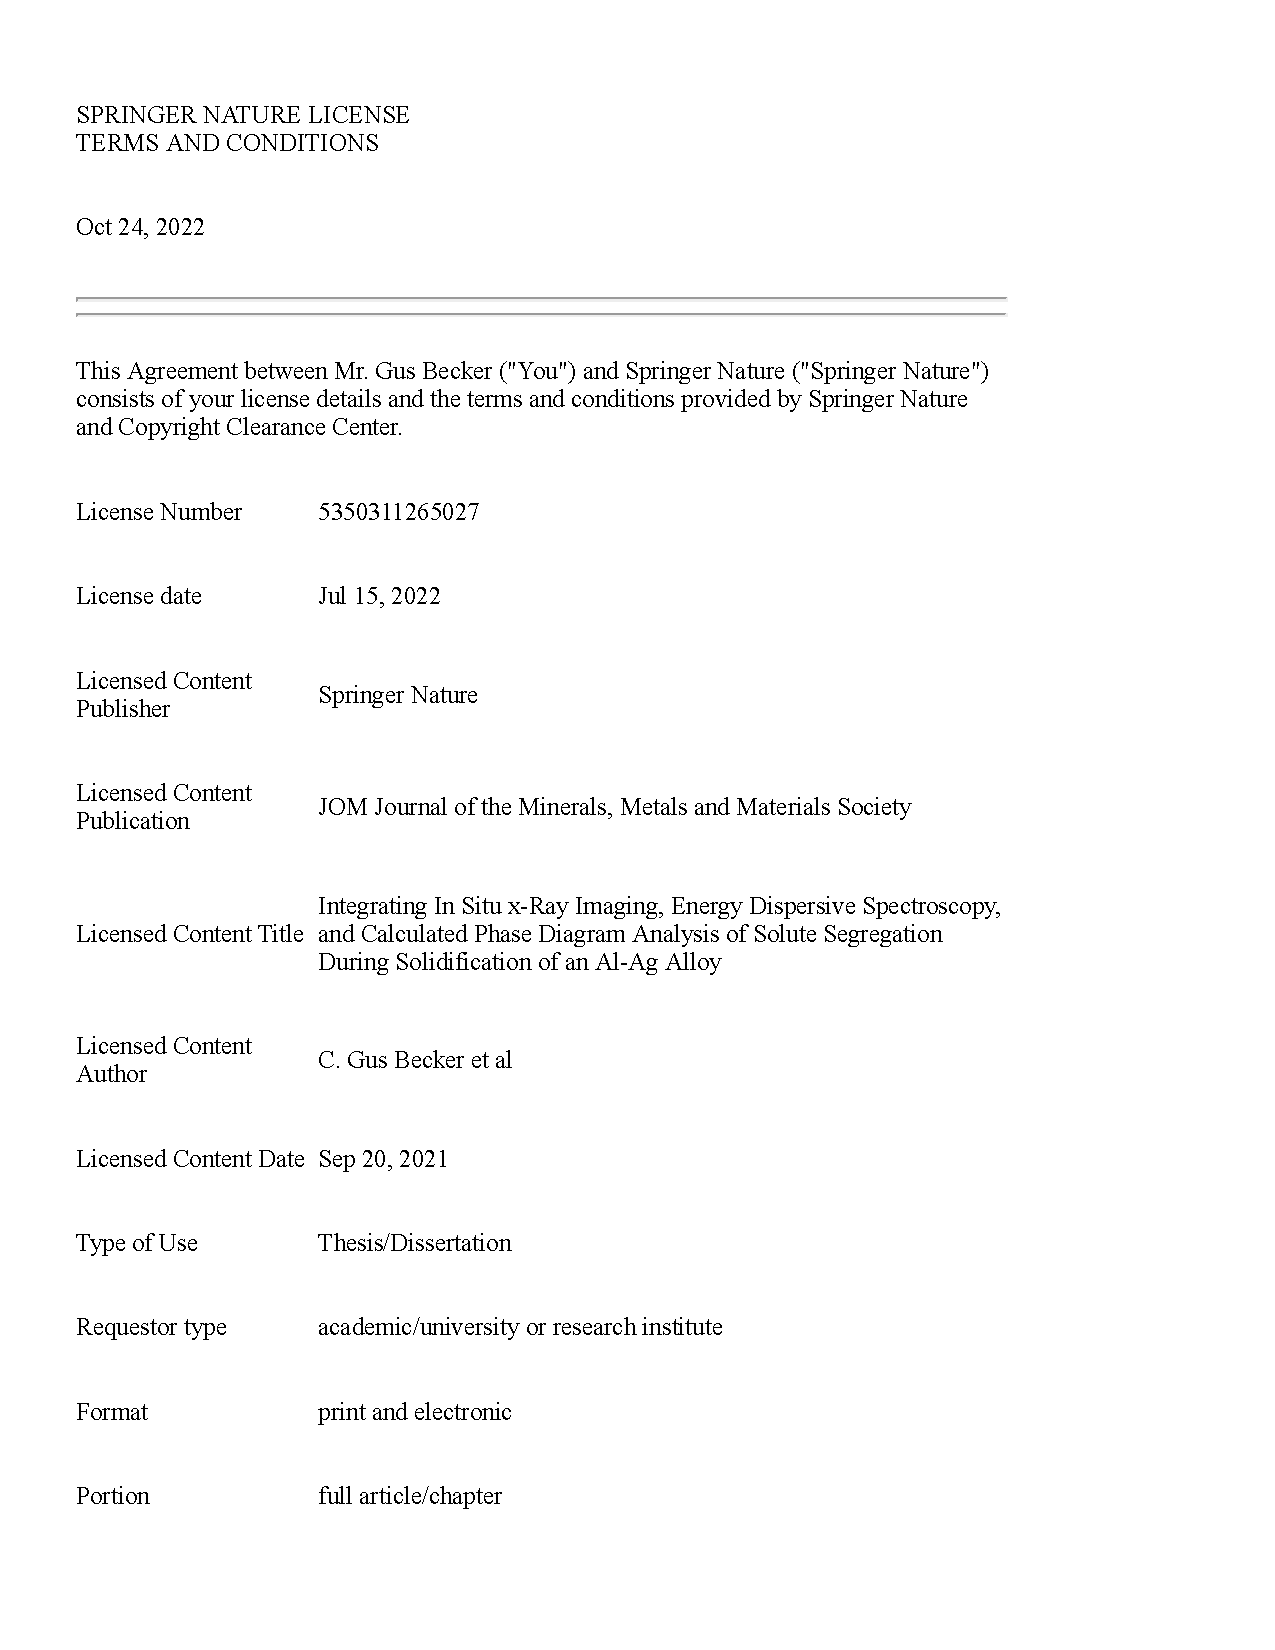
\includepdf[pages={1-6}]{supporting-files/ch3-springer-nature.pdf}
% 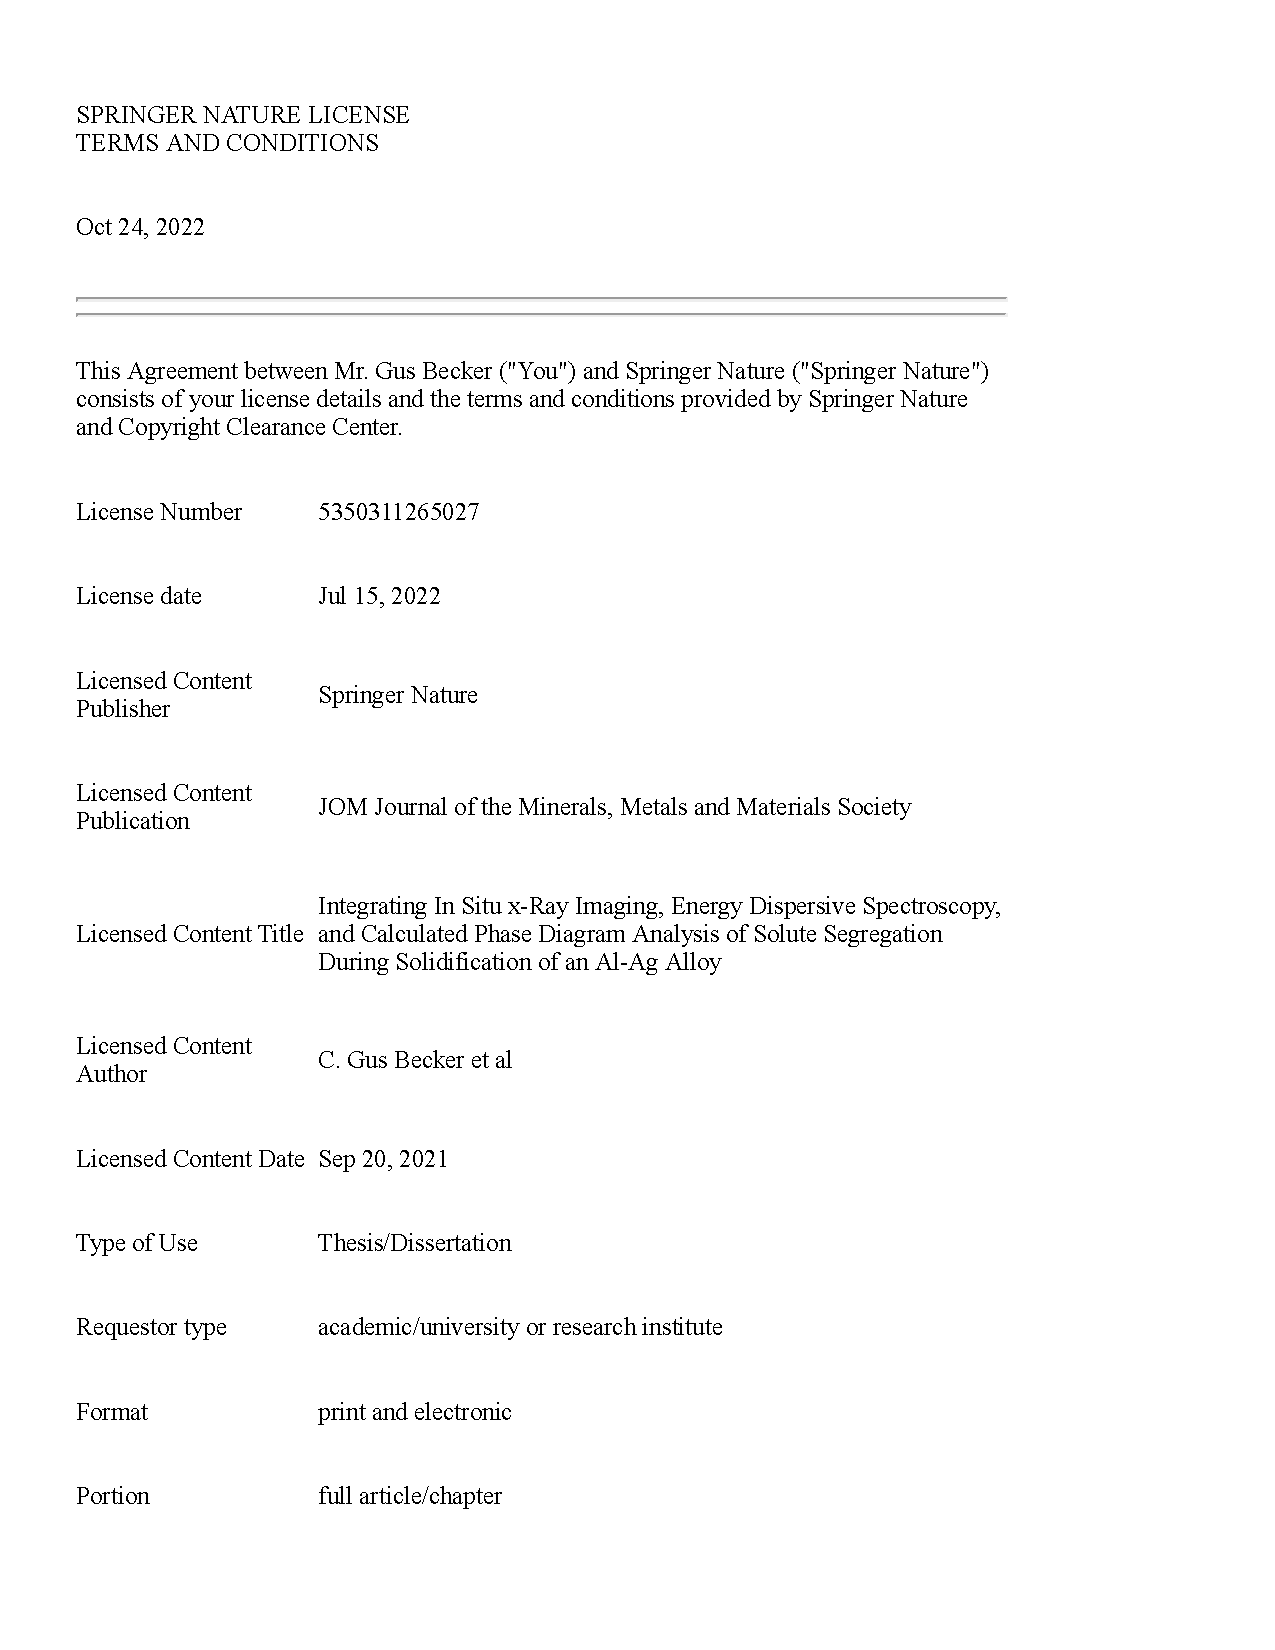
\includegraphics[width=\paperwidth]{supporting-files/ch3-springer-nature.pdf}

\subsection{Permission from Co-Authors}
The following pages express permission from the co-authors of the
journal article in question to reprint the article as part of this thesis.
\newpage
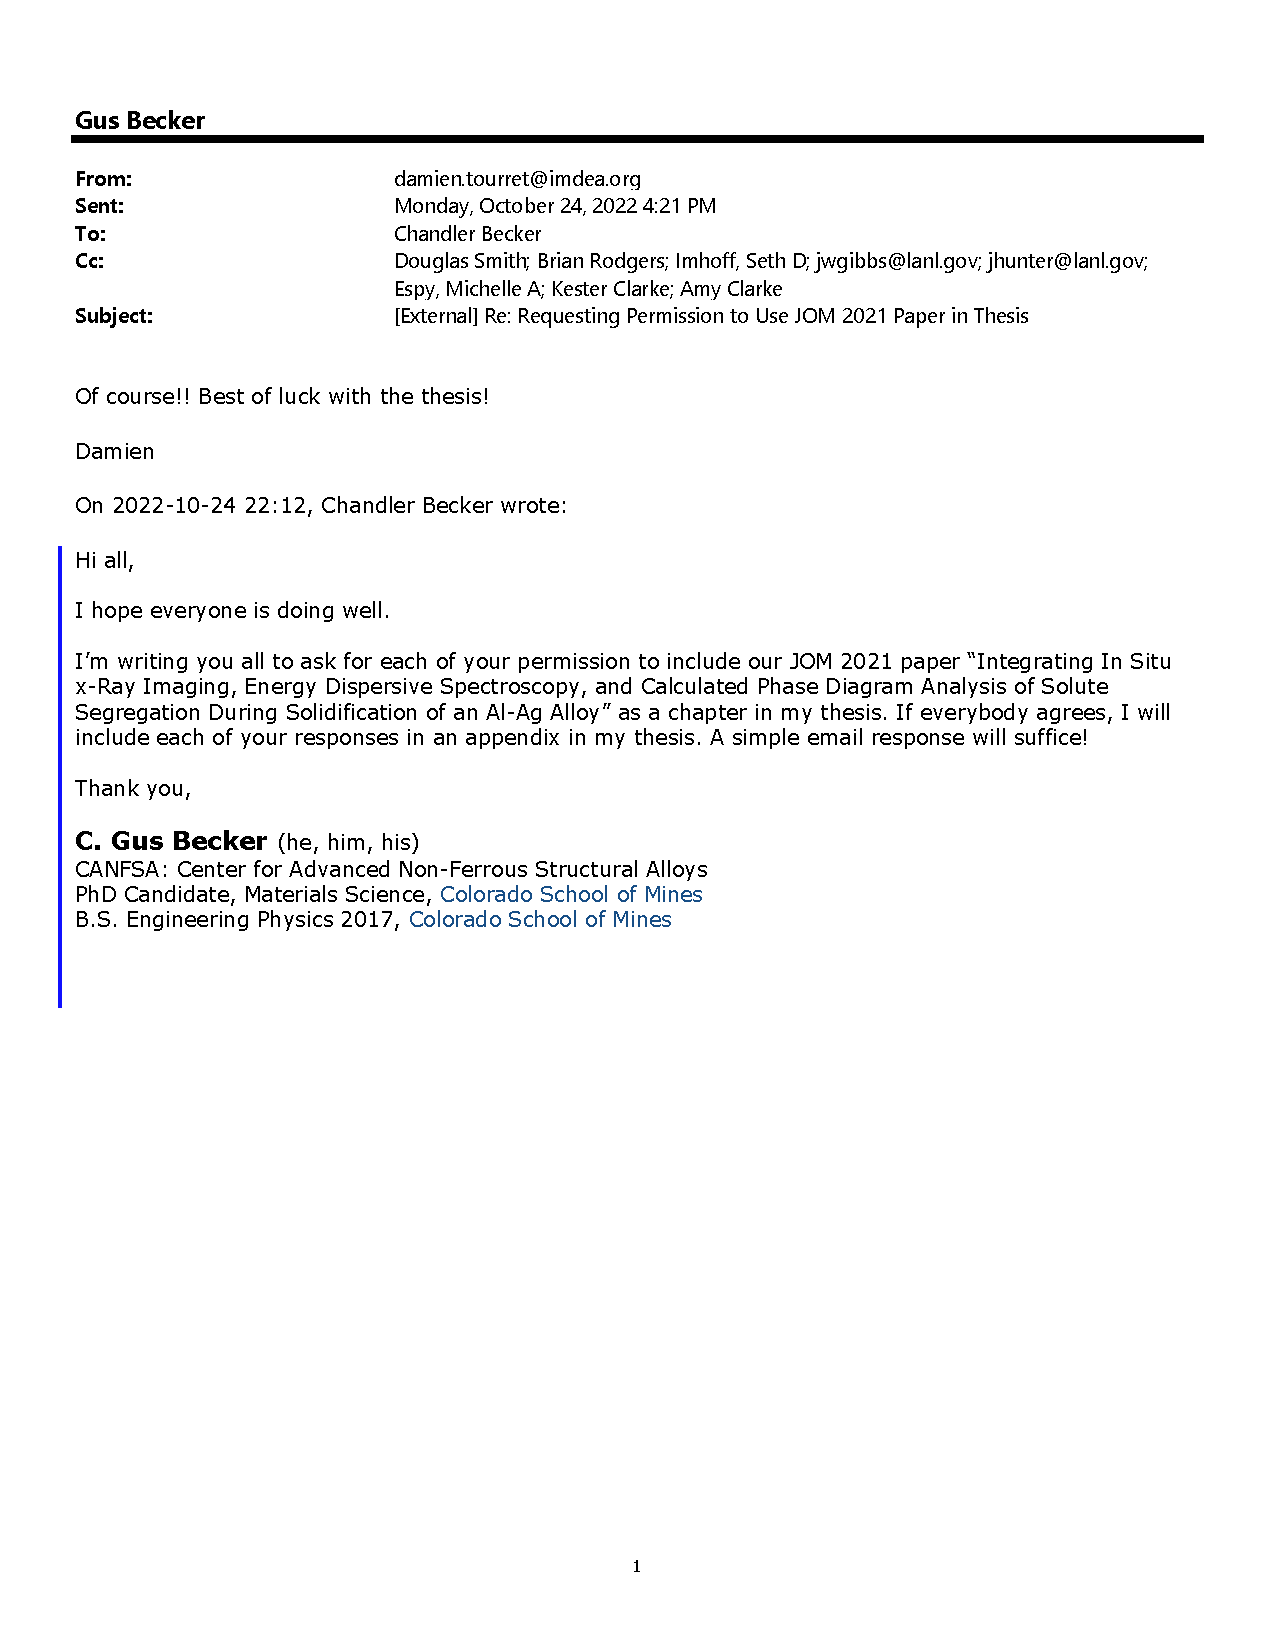
\includepdf{supporting-files/copyright-permissions/ch3-damien-tourret.pdf}
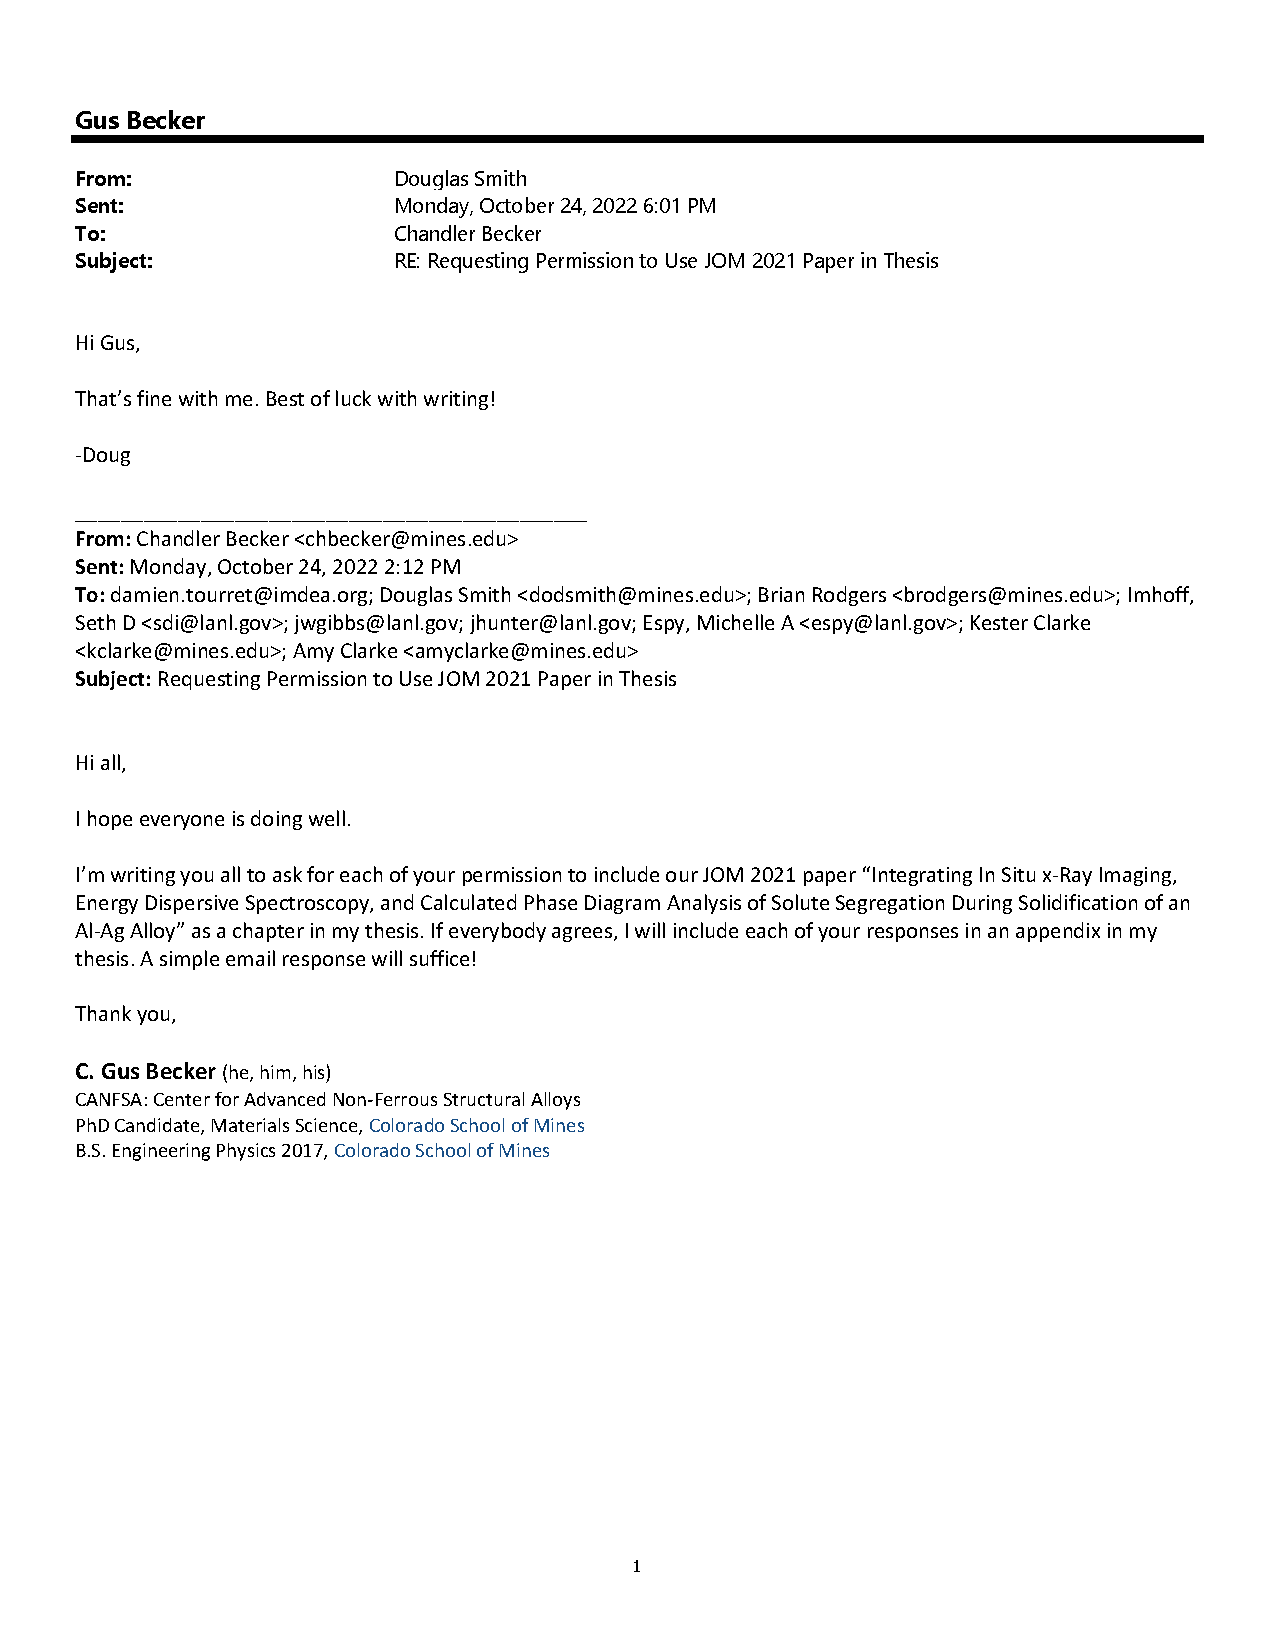
\includepdf{supporting-files/copyright-permissions/ch3-doug-smith.pdf}
\includepdf{supporting-files/copyright-permissions/ch3-brian-rodgers.pdf}
\includepdf{supporting-files/copyright-permissions/ch3-seth-imhoff.pdf}
\includepdf{supporting-files/copyright-permissions/ch3-john-gibbs.pdf}
\includepdf{supporting-files/copyright-permissions/ch3-james-hunter.pdf}
\includepdf{supporting-files/copyright-permissions/ch3-michelle-espy.pdf}



\end{document}